%%%%%%%%%%%%%%%%%%%%%%%%%%%%%%%%%%%%%%%%%
% kaobook
% LaTeX Template
% Version 1.2 (4/1/2020)
%
% This template originates from:
% https://www.LaTeXTemplates.com
%
% For the latest template development version and to make contributions:
% https://github.com/fmarotta/kaobook
%
% Authors:
% Federico Marotta (federicomarotta@mail.com)
% Based on the doctoral thesis of Ken Arroyo Ohori (https://3d.bk.tudelft.nl/ken/en)
% and on the Tufte-LaTeX class.
% Modified for LaTeX Templates by Vel (vel@latextemplates.com)
%
% License:
% CC0 1.0 Universal (see included MANIFEST.md file)
%
%%%%%%%%%%%%%%%%%%%%%%%%%%%%%%%%%%%%%%%%%

%----------------------------------------------------------------------------------------
%	PACKAGES AND OTHER DOCUMENT CONFIGURATIONS
%----------------------------------------------------------------------------------------

\documentclass[
	fontsize=10pt, % Base font size
	twoside=true, % Use different layouts for even and odd pages (in particular, if twoside=true, the margin column will be always on the outside)
	open=any, % If twoside=true, uncomment this to force new chapters to start on any page, not only on right (odd) pages
	%chapterprefix=true, % Uncomment to use the word "Chapter" before chapter numbers everywhere they appear
	%chapterentrydots=true, % Uncomment to output dots from the chapter name to the page number in the table of contents
	numbers=noenddot, % Comment to output dots after chapter numbers; the most common values for this option are: enddot, noenddot and auto (see the KOMAScript documentation for an in-depth explanation)
	%draft=true, % If uncommented, rulers will be added in the header and footer
	%overfullrule=true, % If uncommented, overly long lines will be marked by a black box; useful for correcting spacing problems
]{kaobook}

% Set the language
\usepackage[english]{babel} % Load characters and hyphenation
\usepackage[english=british]{csquotes} % English quotes

% Load packages for testing
\usepackage{blindtext}
%\usepackage{showframe} % Uncomment to show boxes around the text area, margin, header and footer
%\usepackage{showlabels} % Uncomment to output the content of \label commands to the document where they are used

% Load the bibliography package
\usepackage{styles/kaobiblio}
% \usepackage[sorting=nyt,
%             sortcites=true,
%             citestyle=authoryear-comp,
%             bibstyle=authoryear]{styles/kaobiblio}
\addbibresource{main.bib} % Bibliography file

% per fare alberi sintattici
\usepackage{forest}

% aggiunta mia per disegnare alberi sintattici
\usepackage{tikz-qtree}
\tikzset{every tree node/.style={align=center, anchor=north}}

% aggiunta mia per fare la manina di OT
\usepackage{pifont}
 \newcommand{\hand}{\ding{43}}
 
% aggiunta mia per fare strikethrough text
\usepackage[normalem]{ulem} 

% aggiunta mia per fare le colonne tratteggiate nei tableaux OT
\usepackage{arydshln}

% BLOCCO AGGIUNTO PER AVERE LE LETTERONE ALFABETO NELLA BIBLIOGRAFIA
\def\initlist{}
\forcsvlist{\listadd\initlist}{A,B,C,D,E,F,G,H,I,J,K,L,M,N,O,P,Q,R,S,T,U,V,W,X,Y,Z}
\forlistloop{\DeclareBibliographyCategory}{\initlist}
\renewcommand*{\do}[1]{\defbibheading{#1}{\section*{#1}}}
\dolistloop{\initlist}
\AtDataInput{\ifskipbib{}{\addtocategory{\thefield{sortinit}}{\thefield{entrykey}}}}

% COMMENT TO SORT BIBLIOGRAPHY BY CITATION ORDER (otherwise, defaults to option in styles/kaobiblio.sty)
\assignrefcontextentries[]{*}

% Load mathematical packages for theorems and related environments. NOTE: choose only one between 'mdftheorems' and 'plaintheorems'.
\usepackage{styles/mdftheorems}
%\usepackage{styles/plaintheorems}

% aggiunta mia per disegnare grafici in Latex con Tikz
\usepackage{pgfplots}

% aggiunta mia to fit large OT tableaux
\usepackage{adjustbox}

% aggiunta mia per evidenziare testo
\usepackage{soul}

\graphicspath{{examples/documentation/images/}{images/}} % Paths in which to look for images

\makeindex[columns=3, title=Alphabetical Index, intoc] % Make LaTeX produce the files required to compile the index

\makeglossaries % Make LaTeX produce the files required to compile the glossary

\makenomenclature % Make LaTeX produce the files required to compile the nomenclature

% Reset sidenote counter at chapters
%\counterwithin*{sidenote}{chapter}


\def\firstcircle{(90:1.75cm) circle (2.5cm)}
\def\secondcircle{(210:1.75cm) circle (2.5cm)}
\def\thirdcircle{(330:1.75cm) circle (2.5cm)}
%----------------------------------------------------------------------------------------

\begin{document}

%----------------------------------------------------------------------------------------
%	BOOK INFORMATION
%----------------------------------------------------------------------------------------

\titlehead{}
\subject{}

\title[Implicit indefinite objects at the syntax-semantics-pragmatics interface]{Implicit indefinite objects\\ at the syntax-semantics-pragmatics interface:}
\subtitle{a probabilistic model of acceptability judgments}

\author[Giulia Cappelli]{Giulia Cappelli}

% \author[Giulia Cappelli]{Giulia Cappelli \thanks{A \LaTeX\ lover}}

% \date{\today}
\date{Scuola Normale Superiore}

\publishers{in partial fulfillment of the requirements for the degree of Doctor of Philosophy (Ph.D.) in Linguistics}

%----------------------------------------------------------------------------------------

\frontmatter % Denotes the start of the pre-document content, uses roman numerals

%----------------------------------------------------------------------------------------
%	OPENING PAGE
%----------------------------------------------------------------------------------------

%\makeatletter
%\extratitle{
%	% In the title page, the title is vspaced by 9.5\baselineskip
%	\vspace*{9\baselineskip}
%	\vspace*{\parskip}
%	\begin{center}
%		% In the title page, \huge is set after the komafont for title
%		\usekomafont{title}\huge\@title
%	\end{center}
%}
%\makeatother

%----------------------------------------------------------------------------------------
%	COPYRIGHT PAGE
%----------------------------------------------------------------------------------------

\makeatletter
\uppertitleback{\@titlehead} % Header

\lowertitleback{
% 	\textbf{Disclaimer}\\
% 	You can edit this page to suit your needs. For instance, here we have a no copyright statement, a colophon and some other information. This page is based on the corresponding page of Ken Arroyo Ohori's thesis, with minimal changes.
	
% 	\medskip
	
% 	\textbf{No copyright}\\
% 	\cczero\ This book is released into the public domain using the CC0 code. To the extent possible under law, I waive all copyright and related or neighbouring rights to this work.
	
% 	To view a copy of the CC0 code, visit: \\\url{http://creativecommons.org/publicdomain/zero/1.0/}
	
% 	\medskip
	
	\textbf{Colophon} \\
	The data, code, and materials supporting the findings of this dissertation are available within the thesis (and its supplementary materials) or in GitHub repositories referenced in the text.\\ This document was typeset with the help of \href{https://sourceforge.net/projects/koma-script/}{\KOMAScript} and \href{https://www.latex-project.org/}{\LaTeX} using the \href{https://github.com/fmarotta/kaobook/}{kaobook} class. The source code of this book is available at:\\\url{https://github.com/fmarotta/kaobook}
	
	\medskip
	
	\textbf{First version} \\
	First printed in May 2019 \@publishers
}
\makeatother

% ----------------------------------------------------------------------------------------
% 	DEDICATION
% ----------------------------------------------------------------------------------------

\dedication{
	 All models are wrong, but some are useful.\\
	\flushright -- George E. P. Box
}

% ----------------------------------------------------------------------------------------
%	OUTPUT TITLE PAGE AND PREVIOUS
%----------------------------------------------------------------------------------------

% Note that \maketitle outputs the pages before here

% If twoside=false, \uppertitleback and \lowertitleback are not printed
% To overcome this issue, we set twoside=semi just before printing the title pages, and set it back to false just after the title pages
\KOMAoptions{twoside=semi}
\maketitle
\KOMAoptions{twoside=false}

%----------------------------------------------------------------------------------------
%	PREFACE
%----------------------------------------------------------------------------------------

\chapter*{Acknowledgments}
\addcontentsline{toc}{chapter}{Acknowledgments} % Add the preface to the table of contents as a chapter

Acknowledgments

% ringraziare gli open-sourcers e dire che anche io nel mio piccolo sto provando a partecipare al movimento
% e che l'outcome reale del dottorato non è la tesi ma sono io

\begin{flushright}
	\textit{Giulia Cappelli}
\end{flushright}


%----------------------------------------------------------------------------------------
%	TABLE OF CONTENTS & LIST OF FIGURES/TABLES
%----------------------------------------------------------------------------------------

\begingroup % Local scope for the following commands

% Define the style for the TOC, LOF, and LOT
%\setstretch{1} % Uncomment to modify line spacing in the ToC
%\hypersetup{linkcolor=blue} % Uncomment to set the colour of links in the ToC
\setlength{\textheight}{23cm} % Manually adjust the height of the ToC pages

% Turn on compatibility mode for the etoc package
\etocstandarddisplaystyle % "toc display" as if etoc was not loaded
\etocstandardlines % toc lines as if etoc was not loaded

\tableofcontents % Output the table of contents

\listoffigures % Output the list of figures

% Comment both of the following lines to have the LOF and the LOT on different pages
\let\cleardoublepage\bigskip
\let\clearpage\bigskip

\listoftables % Output the list of tables

\endgroup

%----------------------------------------------------------------------------------------
%	MAIN BODY
%----------------------------------------------------------------------------------------

\mainmatter % Denotes the start of the main document content, resets page numbering and uses arabic numbers
\setchapterstyle{kao} % Choose the default chapter heading style

% \chapter*{Acknowledgments}
\addcontentsline{toc}{chapter}{Acknowledgments} % Add the preface to the table of contents as a chapter

Acknowledgments

% ringraziare gli open-sourcers e dire che anche io nel mio piccolo sto provando a partecipare al movimento
% e che l'outcome reale del dottorato non è la tesi ma sono io

\begin{flushright}
	\textit{Giulia Cappelli}
\end{flushright}


\setchapterpreamble[u]{\margintoc}
\chapter{Introduction}
\labch{intro}

\section{Overview} \labsec{intro_intro}

\subsection{Relevance of this thesis}

This thesis is about the omission of direct objects from predicates headed by verbs with two semantic participants, i.e., an Agent (in the syntactic subject position) and a Patient (in the syntactic object position). These "optionally transitive" verbs, deviating from the transitive prototype defined by \textcite{HopperThompson1980}, appear in a wide variety of contexts cross-linguistically, and are licensed by different semantic, aspectual, pragmatic, and discourse factors. Within this broad area of interest, I will focus on \textit{indefinite} null objects, corresponding to what \textcite{Fillmore1986} called "indefinite null complements". These omitted objects, as shown in \ref{introintro1}, refer to something that is "unknown or a matter of indifference" \parencite[96]{Fillmore1986}. Indeed, what matters in the example is that Giulia is writing something, and in particular, something that is usually written. The actual product of the writing event, be it a novel, a shopping list, or a doctoral dissertation, is irrelevant. On the contrary, the referent of \textit{definite} null objects (which I am not studying in this thesis) "must be retrieved from something given in the context", as in \ref{introintro2}. In this case, the context is provided with linguistic means in the first sentence in the example, where a reference is made to grad school. Thus, the omitted object in the second sentence can be understood to refer to a doctoral thesis (the thing one wants to defend soon when in grad school) rather than, say, the title of Olympic champion or the national borders.

\ex. \label{introintro} \a. \label{introintro1} Giulia is writing $\varnothing$\textsubscript{dObj}.
\b. \label{introintro2} Grad school is hard. Giulia hopes to defend $\varnothing$\textsubscript{dObj} soon.

The available literature suggests indefinite object drop to be possible with different types of verbs to varying extents (for instance, change-of-state verbs such as \textit{to kill} are much more resistant to object drop than incremental-theme verbs such as \textit{to eat}), and for any given verb, to be more likely under some specific semantic, aspectual, and pragmatic circumstances. For instance, a direct object can only participate in the indefinite implicit object construction if it is recoverable from the meaning of the verb itself, and transitive verbs are much more likely to be used without a direct object when they are used in imperfective or iterative contexts than in perfective, single-occurrence contexts.\\
While many pages have been written about the role of several linguistic factors in facilitating or blocking indefinite object drop, as I will detail in the first section of this thesis, way fewer attempts have been made to understand the nature of this phenomenon via experimental means, modeling the joint effect of several predictors of object drop. \textcite{Medina2007} made a substantial step in this direction in her (linear) Stochastic Optimality Theoretic model of indefinite object drop in English, taking into consideration the joint effect of object recoverability, telicity, and perfectivity on the grammaticality of indefinite null objects (as gauged via gradient acceptability judgments elicited from native speakers) occurring with 30 transitive verbs. This model shows that:
\begin{itemize}
    \item indefinite object drop is a gradient, non-categorical phenomenon;
    \item it is possible with virtually any transitive verb, but in different degrees depending on the verb semantics;
    \item for any given verb, different aspectual feature may favor or hinder object drop.
\end{itemize}

In the experiments I will perform to study the indefinite implicit object construction, I inherit Medina's methodology and employ the same variant of Stochastic Optimality Theory she devised, with several updates I will illustrate in \refsec{goalsandnovelty} and, in more detail, in the experimental section of this thesis.


\subsection{Main goals and elements of novelty} \labsec{goalsandnovelty}

This thesis is meant as an expansion upon the original model of indefinite object drop designed by \textcite{Medina2007}. I will collect acceptability judgments following her same experimental design and model the data thus collected within the bounds of the same framework (her variant of Stochastic Optimality Theory). In doing so, I add several elements of novelty to the study:
\begin{itemize}
    \item I will model indefinite implicit objects both in English (like Medina did) and in Italian (which is included in such a probabilistic model for the first time), analyzing language-specific differences in the way several factors facilitate object drop;
    \item in addition to using \posscite{Resnik1993} Selectional Preference Strength measure to quantify semantic selectivity (as a proxy to object recoverability), following \textcite{Medina2007}, I will also define a novel computational measure based on distributional semantics (Computational PISA, presented in \textcite{CappelliLenciPISA}) and a behavioral measure (Behavioral PISA) meant to improve on Medina's Object Similarity;
    \item in addition to the three predictors included by Medina in her model (semantic selectivity, telicity, and perfectivity), I will also add iterativity and manner specification as predictors to find out how they affect indefinite object drop and whether a more complex, five-predictor model actually provides a more accurate view on this phenomenon than the original three-predictor model;
    \item in order to make it easier for future research to build on my results (possibly applying my method to other languages, or to the same languages with different predictors) or to replicate them, I intend to share my materials and document my methods (as well as my Python scripts), as detailed in \refsec{supportingmaterials}.
\end{itemize}

Assuming that my probabilistic models of the gradient grammaticality of indefinite object drop are solid, this thesis will be an additional cobblestone on the well-trodden road of studies about indefinite implicit objects, omitted arguments, and transitivity-related phenomena. More in general, it will add to the understanding of the ways several linguistic factors give rise to phenomena that, despite appearing to happen arbitrarily on a lexically-determined basis, are quite systematic in their behavior. Thus, looking at this thesis from a much broader perspective, it can also be argued to be a small, hopefully not insignificant, contribution to research about the systematicity of human language and cognition, and about the interaction of semantic, aspectual, world-knowledge, pragmatic, and discourse factors in determining the way we translate our communicative intentions into syntactically well-formed utterances.


\section{Contents within and without} \labsec{intro_contents}

\subsection{Chapters of the thesis and their structure}
This thesis is divided into two main sections, one devoted to the review of the literature on object drop, Optimality Theory, and gradient models of indefinite null objects (from \refch{objectdrop} to \refch{medina}), and another devoted to my own experiments and the results thereof (from \refch{predictors} to \refch{model}). Let us consider each Chapter in more detail.

\paragraph{Theory and literature review}
In \nrefch{objectdrop} I will define the \textit{indefinite} implicit object construction as a deviation from the transitive prototype (see \refsec{theory_transitivity}) and in contrast with \textit{definite} object drop (see \refsec{theory_def_vs_indef}), based on the literature. In \refsec{theory_defindefinite} I will argue that there is virtually no reason why a transitive verb should not be able to participate in the indefinite implicit object construction (provided favorable aspectual, semantic, and discourse conditions), and that the implicit object is understood to be the prototypical Patient for a given sense of a given verb. In \refsec{theory_entries} I will argue that optionally transitive verbs should only be taken to have a single entry in the lexicon, realized syntactically either with an overt or with an implicit object, rather than having two separate lexical entries. In \refsec{theory_workingdef} I will provide the perspective on indefinite object drop I adopt in my experiments and throughout this thesis.\\
In \nrefch{factors} I will discuss the role played by semantic factors (recoverability, Agent affectedness, and manner specification, in \refsec{semanticfactors}), aspectual factors (telicity and perfectivity, in \refsec{aspectualfactors}), and pragmatic factors (routine, iterativity, habituality, and discourse factors, in \refsec{pragmaticfactors}) in facilitating or blocking object drop with optionally transitive verbs. After some considerations in \refsec{frequencyfail} on the reasons why corpus frequency is not included among the relevant factors, I conclude the Chapter in \refsec{factorsofchoice} with the reasoning behind my choice of predictors of object drop to be used in the experimental section of this thesis.\\
\nrefch{modeltheory} will explain the main tenets of Optimality Theory relative to syntax (in \refsec{classicot}), the reasons why standard Optimality Theory would be a bad fit for a model of the indefinite implicit object construction, and, therefore, why it is advisable to resort to probabilistic models of grammar that are able to account for the gradient grammaticality shown by indefinite object drop, such as Stochastic Optimality Theory (as argued in \refsec{weightedot}).\\
In particular, in this thesis I will adopt the variant of Stochastic Optimality Theory specifically designed by \textcite{Medina2007} to model indefinite object drop, which I describe and discuss in \nrefch{medina}. The contents of the input and the output will be presented in \refsec{inputmedina}. In \refsec{predictorsmedina} I will discuss the implementation of the three predictors the author used in her model (semantic selectivity, telicity, and perfectivity). The probabilistic ranking of the constraints, which I will introduce in \refsec{constraintsmedina}, will be defined in a top-down perspective (from constraint ranking as a function of semantic selectivity to object-drop probability as gradient grammaticality) in \refsec{rankingmedina}, and finally implemented in a bottom-up perspective (from the acceptability judgments to the estimation of parameters of the linear functions) in \refsec{medinacomputation}.

\paragraph{Experiments and results}
\nrefch{predictors} opens the experimental section of this thesis. I will present five facilitating factors (a continuous factor and four binary factors) of object drop I will use as predictors in my Stochastic Optimality Theoretic model, picked among the ones introduced in \refch{factors}. The continuous factor is object recoverability, which I will model via three different measures of semantic selectivity described in \refsec{predictor_sps}, namely \posscite{Resnik1993} Selectional Preference Strength (following \textcite{Medina2007}), Computational PISA (a novel measure based on distributional semantics I contributed to define in \textcite{CappelliLenciPISA}), and Behavioral PISA (a similarity-based measure inspired by Computational PISA and Medina's Object Similarity measure). The four binary factors are telicity in \refsec{predictor_telicity}, perfectivity in \refsec{predictor_perfectivity}, iterativity in \refsec{predictor_iterativity}, and manner specification in \refsec{predictor_mannspec}.\\
In \nrefch{judgments} I will present the materials and methods employed in the behavioral experiments to collect acceptability judgments from native speakers of English and Italian relative to the indefinite implicit object construction. In particular, in \refsec{participants} I will describe how I built the experiment with PsychoPy, how I ran it on Pavlovia, and how I recruited the participants via Prolific. Finally, I will present my 30-verb target dataset in \refsec{verbs}, the experimental design in \refsec{design}, the stimuli in \refsec{stimuli}, and the experimental setting in \refsec{setting}.\\
A first analysis of the data collected with these behavioral experiments will be provided in \nrefch{results}, where I will describe the structure of the Python script I devised to perform the analysis and to compute the models, as well as the procedures of data preprocessing employed (see \refsec{likert_scripts}), before discussing the separate and joint effects of semantic selectivity and the four binary predictors on the acceptability judgments in English and in Italian (see \refsec{eng_judgresult} and \refsec{ita_judgresult}, respectively). In \refsec{sumup_judgresult}, I will argue that the five factors facilitating indefinite object drop are able to predict, to a non-negligible extent, the likelihood a transitive verb will appear without an overt object in a statistical (linear mixed-effects) model, and I will also explain why Medina's variant of Stochastic Optimality Theoretic is a more linguistically-motivated way of modeling these results than the linguistically-naive statistical model.\\
I will define and discuss my Stochastic Optimality Theoretic models of indefinite object drop in English and Italian in \nrefch{model}. In \refsec{introfitting}, I will describe and evaluate my 18 models, stemming from the union of three measures of semantic selectivity, three increasingly more complex constraint sets (Medina's basic set, another with the addition of iterativity, and a full set with manner specification too), and two target languages. In \refsec{stot_full}, I will discuss the theoretical aspects and computational implementation of the two full models of object drop in English and Italian where semantic selectivity is modeled via Behavioral PISA. I will then compare my models with Medina's model and with regression models in \refsec{stot_conclusions}.\\
Finally, I will provide my conclusions and propose some possibile future directions for research about modeling the indefinite implicit object construction in \nrefch{conclusions}.


\subsection{Supporting materials} \labsec{supportingmaterials}
With an eye to the Open Science environment, I used open source software and programming languages to collect and analyse data for this thesis whenever possible, and I am sharing my data, scripts and results on dedicated GitHub repositories. Should anyone in the future read these pages and find themselves interested in replicating my results, or testing new models on the data I collected, or contributing to enrich my repositories, they will be able to do so \href{https://github.com/giuliacappelli}{on my GitHub profile}\sidenote{https://github.com/giuliacappelli}.\\ %  effortlessly (and without spending money on proprietary software)
The interested reader will find my data, i.e., the stimuli for each experiment and the raw results I got from participants, \href{https://github.com/giuliacappelli/dissertationData}{in a dedicated GitHub repository}\sidenote{https://github.com/giuliacappelli/ dissertationData}. In more detail, this repository contains:
\begin{itemize}
    \item 30 target verbs and 10 filler verbs both for English and for Italian, used in all the computational (see \refsec{predictor_sps}) and behavioral (see \refsec{behavPisa} and \refch{judgments}) experiments, as in \refapp{app_verbs};
    \item full lists of the direct objects of each target verb as extracted from the ukWaC corpus for English and from itWaC for Italian, both raw and manually cleaned (as detailed in \refsec{compuPisa});
    \item stimuli, full judgments elicited from 25 participants per language on a 7-point Likert scale, and final scores obtained in the Behavioral PISA experiment (see \refsec{behavPisa}), also provided in \refapp{app_behavPisa};
    \item each verb tagged with its features relative to the verb-specific predictors of object drop, i.e., telicity, manner specification, and semantic selectivity, as in \refapp{app_predictors};
    \item stimuli and full judgments elicited from 30 participants per language on a 7-point Likert scale in the main behavioral experiment of this thesis (see \refch{judgments}), aimed towards creating a Stochastic Optimality Theoretic model of object drop in English and Italian (see \refch{model}), as in \refapp{app_stimuli}.
\end{itemize}
As for the data processing, analysis of results, computational implementation of experimental designs, and creation of stimuli, I coded several Python scripts and documented their usage on GitHub. In detail, they are as follows:
\begin{itemize}    
    \item \href{https://github.com/giuliacappelli/checkPolysemy}{Quantify the polysemy of words in a list}\sidenote{https://github.com/giuliacappelli/ checkPolysemy} using WordNet (Wu-Palmer Similarity), as in \refsec{verbs};
    \item \href{https://github.com/giuliacappelli/behavioralPISA}{Behavioral PISA}\sidenote{https://github.com/giuliacappelli/ behavioralPISA}, a (behavioral) measure of Preference In Selection of Arguments to model verb argument recoverability, as in \refsec{behavPisa}. The script takes care both of creating the stimuli for the experiment and of generating Behavioral PISA scores based on the Likert-scale acceptability judgments provided by human participants;
    \item \href{https://github.com/giuliacappelli/psychopy_exps}{PsychoPy Builder source code}\sidenote{https://github.com/giuliacappelli/ psychopy\_exps} of my behavioral experiments to collect acceptability judgments relative to the indefinite implicit object construction from native speakers of English and Italian, described in \refch{judgments};
    \item \href{https://github.com/giuliacappelli/PsychopyToMedina}{Psychopy-to-Medina converter}\sidenote{https://github.com/giuliacappelli/ PsychopyToMedina}, to convert the output of my PsychoPy behavioral experiment (see \refch{judgments}) into a suitable input for my scripts to analyse the results (see \refch{results}) and create Stochastic OT models of the implicit object construction following \textcite{Medina2007} (see \refch{model});
    \item \href{https://github.com/giuliacappelli/MedinaStochasticOptimalityTheory}{Modeling the grammaticality of implicit objects}\sidenote{https://github.com/giuliacappelli/ MedinaStochasticOptimalityTheory} based on Medina (2007)'s variant of Stochastic Optimality Theory, as in \refch{results} and \refch{model};
    \item \href{https://github.com/giuliacappelli/generateMockLikertGrammaticalityJudgments}{Generate mock Likert-scale acceptability judgments}\sidenote{https://github.com/giuliacappelli/ generateMockLikertGrammaticalityJudgments} based on factor levels specified in the input, to test the above Stochastic Optimality Theoretic model on ideal data before running the experiment proper.
\end{itemize}

\subsection{Published work and outreach}
Relevant parts of the experimental section of this thesis have been shared with the scientific community, both in written form and during conferences. The original distributional measure of Preference In Selection of Arguments (Computational PISA) presented in \textcite{CappelliLenciPISA} and discussed here in \refsec{compuPisa}, tested on large sets of transitive verbs and Instrument verbs in English, was presented at:
\begin{itemize}
    \item *SEM 2020, 9th Joint Conference on Lexical and Computational Semantics, December 12-13th 2020, online due to the Covid-19 pandemic (originally in Barcelona, Spain);
    \item LSA 2021, 95th Annual Meeting of the Linguistic Society of America, January 7-10th 2021, online due to the Covid-19 pandemic (originally in San Francisco, California);
    \item CLiC-it 2020, 7th Italian Conference on Computational Linguistics, March 1-3rd 2021, online due to the Covid-19 pandemic (originally in Bologna, Italy).
\end{itemize}
The results of the main behavioral experiment of this thesis (detailed in \refch{judgments} and \refch{results}), especially the ones pertaining to Italian, were presented at:
\begin{itemize}
    \item SyntOp 2022, Syntactic Optionality in Italian, July 4-5th 2022, Venice (Italy).
\end{itemize}

\pagelayout{wide} % No margins
\addpart{Theory and literature review}
\pagelayout{margin} % Restore margins

\setchapterpreamble[u]{\margintoc}
\chapter{Indefinite object drop} % Object-dropping verbs
\labch{objectdrop}

As mentioned in \refch{intro}, this thesis is about indefinite implicit objects. What is "indefinite" about them? In what sense can they be considered "implicit"? And ultimately, what is objecthood itself? This Chapter will answer these questions in reverse order, from the most general to the most specific one. In \refsec{theory_transitivity} I will make reference to the transitivity continuum, as defined by \textcite{HopperThompson1980} and further explored by later literature. In \refsec{theory_def_vs_indef} a crucial distinction will be made between definite and indefinite object drop, following \textcite{Fillmore1986} and subsequent works. The nature of \textit{indefinite} object drop will be finally described in \refsec{theory_defindefinite} and \refsec{theory_entries}, and a working definition (for the purposes of this thesis) will be provided in \refsec{theory_workingdef}.\\
Before delving into the main contents of the Chapter, a terminological clarification is in order. Throughout this thesis, I refer to an "intransitive" use of transitive verbs to intend the absence of a possible overt syntactic object for verbs which semantically take an Agent and a Patient argument, e.g. \textit{John broke (the window)}. Crucially, I am \textit{not} referring to senses of such verbs where the subject is non-Agentive (e.g. \textit{The ball broke the window}) or to their anticausative uses (e.g. \textit{The window broke}), nor am I referring to verbs that have two semantic participants (an Agent and a Patient) but can only express the internal argument\sidenote{Refer to \textcite{Engelberg2002} for more considerations on the difference between such verbs and the ones exhibiting optional object drop.} (corresponding to the Agent participant) syntactically, such as \textit{to dine}.


\section{Transitivity as a prototype} \labsec{theory_transitivity}

% \subsection{Transitivity in Hopper \& Thompson (1980)} \labsec{theory_ht1980}
School kids everywhere are used to call "transitive" the verbs which take an overt direct object. In a traditional semantic definition, a clause is deemed "transitive" if it describes an event where the action performed by an Agent "passes over"\sidenote{Hence the name of the concept of transitivity, from Latin \textit{transire} 'to go over'.} to a Patient, which usually undergoes some kind of transformation.\\
Going beyond these naive definitions, but still capturing their spirit, \textcite{HopperThompson1980} first proposed an account where transitivity is interpreted as a scalar concept whose strength depends on several parameters, or, to use more modern terminology, as a prototype category \parencite{Naess2007}. In particular, they identified ten parameters \parencite[252]{HopperThompson1980}, reported almost \textit{verbatim} in \reftab{ht1980_parameters}.

\begin{table}[htb] % the "htb" makes table env unfloaty
\caption{\textcite[252]{HopperThompson1980} defined transitivity as a prototype concept determined by ten parameters.}
\labtab{ht1980_parameters}
\begin{tabular}{rl|ll}
 & & \textbf{high transitivity} & \textbf{low transitivity} \\
 \hline
A. & \textbf{Participants} & 2+ (Agent and Object)  & 1 participant  \\
B. & \textbf{Kinesis} & action  & non-action  \\
C. & \textbf{Aspect} & telic  & atelic  \\
D. & \textbf{Punctuality} & punctual  & non-punctual  \\
E. & \textbf{Volitionality} & volitional  & non-volitional  \\
F. & \textbf{Affirmation} & affirmative  & negative  \\
G. & \textbf{Mode} & realis  & irrealis  \\
H. & \textbf{Agency} & A high in potency  & A low in potency   \\
I. & \textbf{Affectedness of O} & O totally affected  & O not affected  \\
J. & \textbf{Individuation of O} & O highly individuated  & O non-individuated  
\end{tabular}
\end{table}

These parameters are potentially active in all languages, but languages may differ from one another with respect to the actual subset of parameters they select as necessary criteria for transitivity. This depends on the "recursivity" \parencite[29]{Naess2007} of prototypical concepts, which assign membership in a category (in this case, transitive clauses) on the basis of attributes which are prototype concepts themselves \parencite[61]{taylor1995linguistic}.\\
Parameters A, B, E, F, and G from \reftab{ht1980_parameters} are self-explanatory. Parameter C (telicity) will be discussed in more detail in \refsec{telicity}. Parameter D (punctuality) refers to the phase between inception and completion of an action, which is non-existent in verbs like \textit{to kick} and obviously present in verbs like \textit{to carry}. Parameter H (agency) separates animate and inanimate subjects. Parameter I (affectedness of the object) determines that sentences like \textit{I drank up the milk} are more transitive than sentences like \textit{I drank some of the milk}, since the milk is only partially affected by the drinking in the latter sentence. Finally, parameter J (individuation of the object) refers to the distinctness of the object both from the Agent and from the background, as summarized in \reftab{ht1980_individuation} \parencite[253]{HopperThompson1980}.

\begin{table}[htb] % the "htb" makes table env unfloaty
\caption{\textcite[252]{HopperThompson1980} defined transitivity as a prototype concept determined by ten parameters.}
\labtab{ht1980_individuation}
\begin{tabular}{c|c}
 \textbf{individuated} & \textbf{non-individuated} \\
 \hline
proper & common \\
human, animate & inanimate \\
concrete & abstract \\
singular & plural \\
count & mass \\
referential, definite & non-referential
\end{tabular}
\end{table}

The individuation parameter is the most controversial among the ten proposed ones, as observed by \textcite[128]{comrie1989language} and later on by \textcite[18]{Naess2007}. According to what has come to be known as "Comrie's generalization", in prototypical transitive clauses both animacy and definiteness are high in the Agent and low in the Patient, \textit{contra} \textcite{HopperThompson1980}. The weak argumentation \textcite{HopperThompson1980} provide in favor of the individuation parameter is that speakers would be more likely to focus on the Patient in \textit{I bumped into Charles} than in \textit{I bumped into the table}, since bumping is more likely to affect human beings than tables. \textcite{comrie1989language} makes a much more compelling point with reference to cross-linguistic typology, basing the generalization on the animacy hierarchy and on referential case-marking (which I will not discuss here, since it would lead me too far from my topic). Later literature \parencite{Naess2007, kemmer1993middle, Kardos2010, Naess2009} reinforced this point by assuming that prototypical transitive events are described by verbs whose subject and object are maximally distinct from a semantic point of view.\\
To sum up, the terse summary by \textcite[15]{Naess2007} clearly shows the relation between the naive definitions of transitivity and the ten-parameter account by \textcite{HopperThompson1980}. A prototypical transitive clause is understood to describe an event such that:
\begin{itemize}
    \item a volitional Agent (E, H)
    \item performs an action (B)
    \item with a tangible, lasting effect on a Patient (A, I, J),
    \item and it is presented as real and completed (C, D, F, G).
\end{itemize}

\textcite[78]{Lorenzetti2008} provides a tighter cluster of parameters, arguing that only a subset of the ones proposed by \textcite{HopperThompson1980} are truly relevant. In particular, the author ditches the criteria relative to the transitive event being real and completed (C, D, F, G), and only keeps agentivity, affectedness, and individuation of the object among the other groups of criteria.


\section{Definite \textit{vs} indefinite drop} \labsec{theory_def_vs_indef}

In \refsec{theory_transitivity} I introduced transitivity as a prototype concept depending on a cluster of parameters and, specifically, involving an Agent acting on a Patient. But what about utterances where events of this kind are expressed without an overt syntactic object? In this Section I will provide an account of the literature on the matter.

\subsection{Either definite or indefinite: discrete accounts} \labsec{theory_discrete}

\paragraph{Introduction}
Verbs behaving intransitively are, using words by \textcite[191]{rutherford1998workbook}, "a mixed bag". Consider, for instance, the examples in \ref{intro}. The sentence in \ref{intro1} features a typical intransitive verb, describing an event where the subject is \textit{not} performing an action with effects on some Patient. The sentence in \ref{intro2} also describes an event where the subject is not volitionally acting on a Patient, but it is nevertheless clear that there has to exist something that John knows (unlike in \ref{intro1}, where there cannot be something that John sleeps). The sentence in \ref{intro3} has an Agent acting volitionally on a Patient, which is however not instantiated syntactically as an overt direct object.

\ex. \label{intro} \a. \label{intro1} John slept.
\b. \label{intro2} John knew.
\c. \label{intro3} John ate.

There is a clear similarity between \ref{intro2} and \ref{intro3}, as opposed to \ref{intro1}. They both require a Patient/Theme semantically \parencite[510]{Somers1984}, and they both surface as object-less syntactically. Quoting \textcite[48]{Yasutake1987}, "they are different from pure intransitives in that the action will not be complete without some lexically implied (but unspecified) object". Oddly, some literature (\textcite{BourmayanRecanati2013, Liu2008} a.o.) does not interpret such verbs as transitive-become-intransitive verbs via the omission of the direct object, but as intransitive-made-transitive verbs. Such an interpretation is totally counter-intuitive and it goes against the generally-accepted tenet that a core feature of so-called "intransitive verbs" is that they have no object slot available in the syntax.\\
There is, however, a crucial difference between \ref{intro2} and \ref{intro3}. Native speakers of English insist that they have to be provided some context in order to understand \ref{intro2} \textemdash what is it exactly that John knew? On the contrary, \ref{intro3} can be interpreted to mean that John had a meal at a certain moment in time, without specifying any additional context. This distinction was captured and defined by \textcite{Fillmore1986} (building upon \textcite{fillmore1969types, Allerton1975}), the established seminal work on the distinction between so-called "definite" and "indefinite" object drop (here represented by \ref{intro2} and \ref{intro3}, respectively).

\paragraph{Fillmore's account}
\textcite[96]{Fillmore1986} distinguishes between Indefinite Null Complements (hence, INC) and Definite Null Complements (hence, DNC) by testing "whether it would sound odd for a speaker to admit ignorance of the identity of the reference of the missing phrase". So, making reference to \ref{intro} again, there would be no issue with saying "John ate. I wonder what he ate.", but it would be quite odd to say "John knew. I wonder what he knew.". Thus, the missing object in \ref{intro2} is a DNC, while the missing object in \ref{intro3} is an INC. Fillmore than splits INCs into two sub-groups based on whether the omitted object is "of considerable generality" or "requiring the specification of various degrees of semantic specialization". The examples in \ref{fillmore} \parencite[96-97]{Fillmore1986} show increasing degrees of, using his words, "semantic specialization". In \ref{fillmore1}, the subject cannot perform the very act of eating or drinking, regardless of the actual ingested item. In \ref{fillmore2} something specific was eaten, but its specific nature is irrelevant inasmuch the speaker is referring to eating as the act of having a meal. In \ref{fillmore3} the omitted object is referring not just to any drinkable liquid, but to alcohol specifically. Finally, in \ref{fillmore4} something very specific was baked by the subject, but this information is backgrounded\sidenote{Refer to \textcite{David2016} for more observations on implicit objects and other omissible elements usually being "the ground in a figure-ground relation".} to focus on the activity itself (I will come back to this in \refsec{theory_incorporation}).

\ex. \label{fillmore} \a. \label{fillmore1} When my tongue was paralyzed I couldn't eat or drink.
\b. \label{fillmore2} We've already eaten.
\c. \label{fillmore3} I've tried to stop drinking.
\d. \label{fillmore4} I spent the afternoon baking.

However, as it will be shown throughout this Chapter, this secondary division of INCs into subgroups does not have to be a binary theoretical distinction. On the contrary, it follows from several finer-grained considerations on the nature of INCs and the factors allowing them. Moreover, this binary division actually opens the door to discussions about a DNC-INC continuum (more details on this in \refsec{theory_continuous}). Specifically, how is "semantic specialization" different from the "knownness" of the object in DNC constructions \parencite[525]{Eu2018}? An answer can be found in \textcite[218]{Allerton1975}, where the case is made that semantically specialized INCs (just like any INC) refer to a category of individuals, while DNCs refer to specific instances of a given category.\\
Going back to the main distinction between INCs and DNCs, finally, \textcite{Fillmore1986} formally defines the former as objects whose "referent's identity is unknown or a matter of indifference" and the latter as objects whose referent "must be retrieved from something \textit{given} in the context". This context "has either to be given linguistically, in the preceding context, or extralinguistically, in the situational context" \parencite[13]{StarkMeier2017}.

\paragraph{Other accounts}
Several other researchers made use of the distinction between definite and indefinite implicit objects brought to the fore by \textcite{Fillmore1986}, providing slightly different definitions which capture different aspects of the phenomenon. \textcite{Allerton1975}, then further developed by Fillmore, distinguishes between "contextual omission" and "lexical omission", which respectively refer to Fillmore's DNCs and INCs. \textcite{CumminsRoberge2004} distinguish between "internally-licensed null objects" (INCs) and "referential null objects" (DNCs). According to \textcite{ruppenhofer2005regularities} and \textcite[30]{PethoKardos2006}, INCs "receive an \textit{existentially quantified} interpretation", while DNCs are "interpreted anaphorically and must therefore have an appropriate antecedent in context to make sense" (\textcite{Fillmore1986} himself referred to this in the title itself, "Pragmatically Controlled Zero Anaphora"). The anaphoric status of DNCs is also central in \textcite{KellerLapata1998}. \textcite[13]{Medina2007}, the foundational work upon which I am basing my own model of the indefinite object construction, sees DNCs as "implicit objects whose particular meaning can be recovered from the preceding discourse or disambiguating physical context" and INCs as "implicit objects whose meaning is recoverable only from the verb in the sentence". Here the focus is all on recoverability, and the author goes on to show that semantic recoverability can be a reliable predictor of object drop in INC sentences. \textcite[293]{Liu2008}, following \textcite{Garcia-VelascoMunoz2002}, takes the shift away from lexical semantics and onto aspectual territory. In particular, the point is made that INCs involve a change of focus "from the object in the transitive use to the activity (the verb) itself in the intransitive use" (an idea that I will discuss in full detail in \refsec{theory_incorporation}), while DNCs do not determine such a shift.\\
The accounts provided so far are not in conflict with Fillmore's formulation of the problem at hand, nor are they in conflict with the view I am adopting in this thesis in order to provide a probabilistic model of the implicit object construction. Other accounts, on the other hand, are more challenging and deserve a more thorough clarification. Let us consider the most relevant ones for my argumentation.\\
\textcite[55]{TonelliDelmonte2011} argue that, while INCs are "constructionally licensed, in that they apply to any predicate in a particular grammatical construction", DNCs are "lexically specific, in that they apply only to some predicates". Later in this Section (on \refpage{recipes}) and in \refsec{theory_continuous} I will bring evidence in support of the opposite point of view, which is in favor of seeing DNCs as (extra- and intra-linguistically) contextually, not lexically, determined. Moreover, \posscite{TonelliDelmonte2011} account is in direct conflict with \textcite[95]{Fillmore1986}, who argues that INCs are "limited to particular lexically defined environments" (such as the object slot of \textit{to eat} and \textit{to read}). In this regard, I side with \textcite{TonelliDelmonte2011}. My probabilistic model of INCs (the results thereof are discussed in \refch{results} and modeled in \refch{model}) will provide strong evidence in support of the idea that any transitive verb can participate in INC constructions, provided the right aspectual, semantic, and pragmatic features. Indeed, as noted by \textcite[216]{HuddlestonEtAl2002}, transitivity is better thought of as a property of verb \textit{use}, rather than a feature of verbs themselves.\\
In a pragmatic (in particular, not lexical) perspective, \textcite[44]{AnderBois} and \textcite[53-54]{Melchin2019} both stay true to Fillmore's original interpretation of DNCs as "pragmatic anaphoras", arguing that DNCs corefer with other referents in the discourse. Moreover, they maintain that INCs lack the possibility of having coreferential interpretations. Fillmore himself \parencite[97]{Fillmore1986} made this point with example \ref{coref}, where \ref{coref2} cannot be considered a proper answer to the question in \ref{coref1}. This is taken to mean that there is no co-reference between the sandwich and the implicit object of \textit{to eat} in \ref{coref2}.

\ex. \label{coref} \a. \label{coref1} What happened to my sandwich?
\b. \label{coref2} *Fido ate.

However, examples can be provided in support of the opposite. \textcite[142-144]{groefsema1995understood} makes use of sentences such as the one in \ref{groefsema} to argue that INCs can indeed refer to specific individuals, provided sufficient linguistic context. As \textcite[168]{scott2006less} observes, omissions of this kind "allow the speaker's meaning to hover between the definite and indefinite readings", so that the interpretation the hearer applies to the omitted object is "specific yet indefinite". I will come back to other blurred distinctions between definite and indefinite object drop in \refsec{theory_continuous}.

% \ex. \label{groefsema} \a. \label{groefsema1} John brought the sandwiches and Ann ate.
% \b. \label{groefsema2} John picked up the glass of beer and drank.

\ex. \label{groefsema} John picked up the glass of beer and drank.

Nevertheless, this account does not disrupt Fillmore's foundation. As explained by \textcite[527]{Eu2018}, not even in sentences like \ref{groefsema} do INCs force the identification of a specific referent. What happens, instead, is that native speakers processing INCs in a flexible context of this kind can be induced to understand the missing object as if co-referring to the previously mentioned one. Thus, INCs can grammatically dissociate the mentioned referent from the one implied by the missing object, while this possibility is not active for DNCs (which are always co-referential, regardless of the context). Considering eventualities like this, it really is no wonder that \textcite[110]{Cote1996}, with respect to implicit objects in English, spoke of "murky water" in relation to the distinction between lexically-provided information and context available via world knowledge.



\paragraph{Genre-based implicit objects: a special case of definite object drop} \labpage{recipes}

I will now discuss genre-based implicit objects, a type of DNCs whose very existence goes in favor of DNCs being virtually possible with any verb, provided it appears in a discourse context that is conducive to object omission (\textit{contra} \textcite[55]{TonelliDelmonte2011}, \textit{pro} \textcite{Goldberg2001}). To quote \textcite[175]{RuppenhoferMichaelis2010}, "argument omission can but need not be licensed by a lexeme". This possibility was first observed by \textcite[95]{Fillmore1986}, who acknowledged that in "certain kinds of highly restricted mini-genres" (e.g. instructional imperatives in recipes) the omission of objects and other non-subject complements is not lexically determined (see also \textcite[237]{Haegeman1987}). Crucially, it is not the case that there is a special grammar of recipe contexts that supersedes the actual grammar of the language the recipe uses \parencite{Culy1996, Cote1996}. On the contrary, recipes and other specialized genres just serve to provide an encompassing discourse and world-knowledge context to the listener/reader. Not only that, but genres are so intertwined with argument omission that it is sometimes possible to evoke a genre just by performing the right kind of DNC, as \textcite[159]{RuppenhoferMichaelis2010} exemplify by making reference to the title of a novel by Cynthia P. Lawrence, "Chill $\varnothing$ before Serving $\varnothing$: A Mystery Novel for Food Lovers" (a clear reference to instructional imperatives found in recipes).\\
Many linguistic analyses of DNCs licensed in "mini-genres" focus on recipe contexts \parencite{Ahringberg2015, Garcia-VelascoMunoz2002, Megitt2019, Ruda2014, MassamRoberge1989, Bender, Culy1996, Massam1992,  PaulMassam2021recipes}. In particular, \textcite{Culy1996} performed a multiple regression analysis on diachronic sets of contemporary and historical recipes with several predictors, finding that the style of a recipe book and discourse factors are the most important predictors of recipe DNCs.\\
Other authors provided accounts pertaining to a broader spectrum of genres. For instance, in addition to recipes, \textcite{Cote1996} also considers "telegraphese", i.e. the telegraphic register used in telegraphs, memos, and signs. \textcite{Weir2017} focuses on what he calls "reduced written register" in English, i.e. the absence of objects in recipes, instructional/directive imperatives\sidenote{As noted by \textcite[162]{RuppenhoferMichaelis2010}, non-instructional imperatives cannot participate in DNC constructions, as shown in their example \textit{Take *(the money) and run}.}, diaries, text messages, internet-based communication, and similar contexts. The presence of DNCs in text messages and internet-based communication is further explored by \textcite{StarkMeier2017} and \textcite{Stuntebeck2018}, focusing on Whatsapp messages. \textcite[304]{Liu2008} mentions instructional languages, such as that found on manuals, warning signs, and product labels. \textcite{Paesani2006} provides a thorough account of object (and subject) drop in special registers (such as recipes, diaries, and headlines), noting clear similarities between DNCs in recipes and the broader phenomenon of Topic drop \parencite[165]{Paesani2006}. Focusing instead on non-contemporary language found in historical texts, it is possible to find studies by \textcite{Almeida2009} on Middle English medical texts, and by \textcite{Korkiakangas2018} on Early Medieval documentary Latin.\\
In an unconventional account of football language, \textcite{BerghOhlander2016} argue that verbs licensing DNCs are "monotransitives" \parencite[54]{quirk1985grammar} in this sublanguage, since they can only take one argument. Let us consider the examples in \ref{berghohlander}.

\ex. \label{berghohlander} \a. \label{berghohlander1} Iniesta passed (the ball) and Messi finished (the attack) clinically.
\b. \label{berghohlander2} John passed *(the salt) and finished *(his steak).

In \ref{berghohlander1}, the direct objects can be omitted because the two footballers are performing acts that need no further explanation in the football community. In this game, you can only pass balls and finish attacks. Incidentally, \textcite[266]{Dvorak2017thesis} notes something similar about some verbs in Czech (e.g. \textit{smeknout} 'to uncap, to tip' the hat one is wearing, \textit{zaparkovat} 'to park' the vehicle one is driving) having "idiomatized meanings [...] limited to a particular jargon or slang" and, crucially, allowing "only one particular entity in the role of an internal argument".\\
Moreover, given the presence of a single ball against many players, match reports are much more likely to DNC the ball rather than the footballers, as observed by \textcite[167]{RuppenhoferMichaelis2010} and \textcite{ebeling2021score}. On the contrary, in the probable context of a dinner in \ref{berghohlander2}, it is not possible to say that John just "passed" or "finished", let alone clinically. \textcite[22]{BerghOhlander2016} explain the existence of DNCs in football reports (and, more generally, object omission) as a manifestation of the "principle of least effort" \parencite{zipf1949leasteffort} and also of the Gricean pragmatic maxim of quantity, which compels speakers to avoid being more informative than necessary. However, as \textcite[166]{RuppenhoferMichaelis2010} observed before, "genre-based omissions are never obligatory", since the maxim of quantity (favoring implicit objects) is counterbalanced by the need for informativeness (favoring overt objects).


\subsection{Neither definite nor indefinite: continuous accounts} \labsec{theory_continuous}

The account of genre-determined DNCs offered in \refsec{theory_discrete} opens the door to a broader discussion of \posscite{Fillmore1986} distinction between definite and indefinite omitted objects. As argued in \textcite[165]{RuppenhoferMichaelis2010} and \textcite[24]{BerghOhlander2016}, the main factor allowing for an object to be omitted is its recoverability (refer to \refsec{recoverability} for a full discussion), which depends on linguistic aspects as well as on contextual and discourse factors, and on world knowledge too. Focusing on recoverability makes it possible to go beyond the binary distinction between INCs and DNCs provided by \textcite{Fillmore1986} and many others, and also beyond the need to postulate verb-specific object-dropping capabilities. In particular, it paves the way for a non-binary account of object drop, where no clear-cut distinction between two types of omission have to be postulated (something that, in essence, was already implicit in \posscite{HopperThompson1980} assumptions).\\
If recoverability is the cornerstone of object-droppability, and if it is a scalar, or even graded, feature of objects, then it stands to reason that object-droppability itself is a graded phenomenon. Taking a small step forward in this direction, \textcite{AnderBois} posits the existence of "flexible implicit arguments" to explain sentences like \textit{The Giants won $\varnothing$}, whose implicit object has a referent known to the reader (as with DNCs), which is, crucially, known because of world knowledge\sidenote{In this case, world knowledge about American football.} and not because of the presence of a linguistic antecedent (as with INCs). \textcite{CumminsRoberge2005} provide what they call a "modular account" of null objects in French, stemming from the intersection of several syntactic, semantic, pragmatic and discourse factors (a similar account of object drop, still abiding to Fillmore's binary distinction, is provided by \textcite{Cennamo2017}).\\
A more cogent, continuous account is offered by \textcite{Glass2013}, who acknowledges that there is "plenty of middle ground" between minimum recoverability (an object has to exist but it is unknown) and maximum recoverability (the specific identity of the object is known). In particular, she argues that, in order to be omitted, an object just has to be sufficiently recoverable for speakers to communicate felicitously, and that community- or genre-specific sublanguages are more prone to certain kinds of object omission simply because those smaller contexts favor object recoverability. Moreover, she explicitly argues against an INC-DNC distinction \parencite[1]{Glass2013}. A pioneering attempt to bring evidence in favor of the intuition that recoverability is the key in object omission is found in \textcite{Resnik1993, Resnik1996}, an information-theoretic account of selectional constraints testing, among other things, the relationship between transitivity and discourse context (more on Resnik's method in \refsec{resnik_sps}).\\
As I will argue later in \refsec{theory_workingdef}, I stay agnostic with respect to the binary or continuous nature of object-droppability in my account of indefinite null objects. Following binary accounts, such a study would simply be a matter of considering those factors which are known to favor the emergence of INCs. On the other hand, under continuous-droppability assumptions, it would be a more complex matter of modeling both contexts and linguistic factors determining any kind of object drop, trying to position implicit null objects in a specific portion of the object-droppability spectrum.


\section{Defining the indefinite} \labsec{theory_defindefinite}

In this Section I will delve into a detailed discussion on indefinite implicit objects, the focus of this dissertation. In \refsec{theory_def_vs_indef} I reported a series of both now-classic and more recent accounts of the differences between so-called definite and indefinite null objects. Let us now comment on the nature of the latter, which were given several labels in the literature (objects of "detransitive verbs" in \textcite[46]{Yasutake1987}, "implicit objects" in \textcite{Glass2013} and \textcite[29]{PethoKardos2006}, or "pseudo-intransitive", "labile", "ambitransitive", "null complements", "understood arguments", "unspecified objects", "null instantiations" in other authors).

% \subsection{The involved parties} 

\subsection{Which verbs?} \labsec{whichverbs}

Traditionally (\textit{contra} this thesis and \textcite[55]{TonelliDelmonte2011}, among others), indefinite null objects are taken to only be possible with a restricted set of activity verbs. For instance, \textcite[510]{Rizzi1986} provides an argument in favor of indefinite object drop being "lexically governed" in English on the basis that in some pairs of semantically related verbs (e.g. \textit{to eat} and \textit{to devour}) one member of the pair allows for object drop, while the other does not. \textcite[236]{Haegeman1987} does not hesitate to define this account "convincing", and similar notes are also found in \textcite{Fillmore1986, Rice1988, Mittwoch2005, Gillon2012}. I will come back on the theory referring to specific case of these "semantic minimal pairs" in \refsec{mannerspec}. The important aspect, here, is that traditional or traditionally-leaning literature\sidenote{Such as \textcite{RuppenhoferMichaelis2014}, arguing that object drop is "an aspect of argument realization licensed by lexemes, which may differ from one another in idiosyncratic ways".} has trouble motivating indefinite implicit objects on the basis of meaning alone, but it also needs it to be lexically determined. With that said, which verbs does then the literature identify as allowing indefinite object drop?\\
First of all, the verbs under consideration drop \textit{syntactic} arguments, crucially, not \textit{semantic} ones. In other words, indefinite object drop are obligatory semantic arguments of such verbs \parencite[120]{Cote1996}, while they do not surface syntactically (more on the syntax of indefinite implicit objects in \refsec{theory_incorporation}). \textcite[134]{Jackendoff2003} specifically observes that it is quite inaccurate to say that such verbs "license an optional argument", since this definition "conflates semantic and syntactic argument structure". He illustrates this point by comparing \textit{to eat} and \textit{to swallow} in \ref{eatswallow}. Both show identical syntactic behavior, but while it is possible to swallow without swallowing anything\sidenote{If one does not consider saliva.}, it is not possible to eat without eating something.

\ex. \label{eatswallow} \a. \label{eatswallow1} Bill ate (the food).
\b. \label{eatswallow2} Bill swallowed (the food).

Another key point in traditional literature on indefinite implicit objects concerns the difference between change-of-state verbs (such as \textit{to break, to harden, to open}) and pseudo-transitive verbs (such as \textit{to eat, to write, to sweep}). Verbs belonging to the former class are prototypically transitive \parencite{HopperThompson1980, Kardos2010, lemmens2006}, since they feature two maximally distinct arguments (a volitional Agent subject and a non-volitional Patient object), while verbs belonging to the latter class exhibit both transitive and intransitive features \parencite{Armstrong2011}. Thus, only pseudo-transitives can license indefinite null objects in this dichotomy. They also appear to be a semantically rich class, comprising verbs of creation (e.g. \textit{to cook, to write, to knit}), verbs of ingestion or consumption (e.g. \textit{to eat, to drink}), and verbs of surface contact (e.g. \textit{to sweep}). While syntactically they have their ambivalent behavior in common, semantically they share the fact that their objects all are "incremental themes"\sidenote{Please refer to \textcite[279]{RappaportHovavLevin2005} and \textcite[4]{Kardos2010} for an extensive account of incremental themes.}, a term originally proposed by \textcite{dowty1991thematic} to refer to verbs showing homomorphism between the physical extent of their object and the temporal progress of the event. Thus, \textit{to eat} is an incremental-theme verb because the Patient gets progressively smaller while ingested by the Agent, \textit{to write} because the Theme gets progressively more wordy while the Agent types or pens it, and so on. On the contrary, \textit{pace} Dowty's attempt to apply this analysis to change-of-state verbs \parencite[568]{dowty1991thematic}, \textit{to close} is not an incremental-theme verb because sentences like \textit{Matt closed the door half-way} do not entail that half the door was closed \parencite[279]{RappaportHovavLevin2005}. Since incremental-theme verbs can behave both transitively and intransitively, in \textcite[33]{Levin1993} they are said to participate in the "unspecified object alternation". The author also provides a list of more than 40 verbs allowing for indefinite object drop, an event which \textcite[116]{Dvorak2017} praises as a major breakthrough after previous literature only focusing, "somewhat disturbingly", on the sole verb \textit{to eat}\sidenote{An unfortunate choice for a single example of the whole category of object-dropping verbs, as we will see later in \refsec{theory_incorporation}.}.\\
As I will show with the probabilistic model of indefinite null objects I define in this dissertation (final results presented in \refch{model}), object drop is possible both with change-of-state verbs and with incremental-theme verbs, the difference being a matter of degrees (determined by several linguistic factors, see \refch{factors} and \refch{predictors}), not a binary feature as in traditional accounts.


\subsection{Which objects?} \labsec{whichobjects}

While syntactically unexpressed and semantically unspecified (at least with respect to a specific entity), indefinite implicit objects of the verbs allowing them still have to refer to \textit{something}. To what, though? Is it possible to generalize the answer?

\paragraph{Omitting \textit{something}}
This \textit{something} that object-dropping verbs refer to has been interpreted quite literally in traditional literature on the issue. \textcite{KatzPostal1967integrated} and \textcite{FraserRoss1970idioms} distinguish between the deletion of \textit{it} (expressed by the constructions which \textcite{fillmore1969types, Fillmore1986} made known as "definite null complements") and the deletion of \textit{something} (expressed by indefinite null objects). A similar consideration is also found, in passing, in \textcite[30]{PethoKardos2006} and in \textcite[6]{Ahringberg2015}.\\
However, several objections can be made to this idea. Historically, the first came from \textcite{Mittwoch1982, Mittwoch2005}, who argued that the omitted object cannot be \textit{something} because "this would be incompatible with the atelic nature of the resulting sentence". I will come back to telicity, and the somewhat different approach I will embrace in the next Chapters, in \refsec{telicity}. Other authors \parencite{Marti2015, fodor1980functional, Melchin2019, Gillon2012, Gillon2006english, gillon2011french, Dvorak2017, Lasersohn1993, CondoravdiGawron1996} argue instead that indefinite implicit objects have to be interpreted as "weak indefinites" \parencite[55]{Melchin2019} as bare masses and plurals, instead of the indefinite pronoun \textit{something}, because only the former have obligatory narrow scope with respect to other quantifiers in the sentence (a behavior shown by indefinite null objects)\sidenote{Please refer to \textcite{carnie2021syntax}, a thorough handbook of generative syntax, for a gentle introduction to scope-taking constituents and the use of logic operators in syntax.}. Let us consider the examples in \ref{scope}, taken from \parencite[55]{Melchin2019}. In \ref{scope1} only the universal quantifier in the subject can take wide scope and the implicit object has to take the lowest scope, while in \ref{scope2} either the universal quantifier in the subject or the existential quantifier in the object can take wide scope.

\ex. \label{scope} \a. \label{scope1} Everyone ate. \hfill $\forall$ > $\exists$ / \# $\exists$ > $\forall$
\b. \label{scope2} Everyone ate something. \hfill $\forall$ > $\exists$ / $\exists$ > $\forall$

Let us unpack this notation. This means that in \ref{scope1}, for every (universal quantifier $\forall$) person, there exists some edible entity that was eaten. In \ref{scope2} this interpretation is possible too, as well as the wide-scope-existential interpretation. In this second reading, which appears to be less perspicuous than the other, for some edible item (existential quantifier $\exists$), every person ate it.\\
The observation that indefinite implicit objects can only take low scope also holds with respect to other logic operators than quantifiers. For instance, \textcite[316]{Gillon2012} provides example \ref{gillon_neg} about negation, where the operator is shown to take obligatory wide scope over the sentence.

\ex. \label{gillon_neg} Bill did not read. \hfill $\neg \exists$x Rbx / \# $\exists$x $\neg$Rbx

This means that the only possible interpretation of this sentence is that Bill did not read anything (the first proposed truth condition of the sentence), not that there exists something that Bill did not read (the second truth condition, marked as improper).\\
Therefore, indefinite implicit objects have to be interpreted as weak indefinites (bare masses or plurals), not as the pronoun \textit{something}. However, it is clear that not \textit{any} weak indefinite can be interpreted as the omitted object of a given verb. Which ones are the right ones? I am now going to provide some answers based on the literature.

\paragraph{Prototypical objects}

\textcite[122]{vanvalinlapolla1997syntax} coined the term "inherent arguments" to describe the indefinite implicit objects occurring with activity verbs, based on the idea that they denote a facet of the meaning of the verb, characterizing the action itself rather than a participant. I will devote some space to a detailed discussion of intransitivization as a means to focus on the activity itself on \refpage{activityfocus}. Resorting once again to the concept of linguistic prototype, which is indeed central in this discussion of transitivity (\refsec{theory_transitivity}) and object drop, much literature agrees on indefinite null objects being understood as prototypical\sidenote{Note that while all referenced works appeal to the notion of prototypical argument, not all of them phrase this idea exactly in these terms. Some refer to "implied arguments", "default interpretations", "standard objects", "understood object", and other labels in the same vein.} arguments of the verb \parencite{Rice1988, Naess2007, bresnan1978realistic, Melchin2019, Mittwoch2005, Dvorak2017thesis, Levin1993, Lorenzetti2008, quirk1985grammar}. However, what is a prototypical object of a given transitive verb? \textcite[204]{Rice1988} provides the examples in \ref{rice}.

\ex. \label{rice} \a. \label{rice1} John smokes (cigarettes / *Marlboros / *a pipe / *SMOKING MATERIALS).
\b. \label{rice2} John drinks (alcohol / *gin / *water / *coffee / *LIQUIDS).
\c. \label{rice3} When he goes to Boston, John drives (a car / *a Toyota / *a motorcycle / *A VEHICLE).
\d. \label{rice4} Each afternoon, John reads (a book / *Ulysses / *the newspaper / *PRINTED MATTER).

Examples in \ref{rice1}, \ref{rice3}, and \ref{rice4} all appeal to our world knowledge, in particular, to our knowledge of what is the most probable choice of the average Joe (or John, in these examples). People usually smoke cigarettes which do not have to be necessarily Marlboros, they drive differently branded cars in their trips out of town, and they like to read generic books in the afternoon\sidenote{Apparently, for many people, especially the ones still liking their news to be printed on paper, reading the news is a leisurely activity to be specifically enjoyed in the mornings while having breakfast. This habit had to be even more common in the late '80s than today.}.\\
As noted by \textcite[125]{Naess2007}, however, example \ref{rice2} poses a challenge to the protypicality-enabled omission theory. The most typical liquid one can drink is usually water, not alcohol. And if one was to understand that the omitted substance is alcohol due to its very omission, would not this argumentation become circular?\sidenote{See also \textcite[20]{Mittwoch2005} on the issue of circularity.} The problem alcohol poses for linguists (or better, for linguistic theory) can be explained from different angles. I, for one, would appeal to the gricean maxim of relevance, in that water is indeed the typical liquid we drink, but it is so much typical (being necessary for good health and even life) that it would be actually weird to mention water-drinking in casual conversation. No one would bat an eye at John drinking water, so it would make little sense to utter \ref{rice2} implying water-drinking. Indeed, we only refer to the act of drinking water when it becomes relevant, for instance during hot summers (\textit{Remember to drink!}) or on a Sunday morning (\textit{I am so glad I drank water before going to bed.}). Thus, since the only socially relevant, statistically likely, choice of a drink for John in \ref{rice2} is alcohol, that is what we intend as a prototypical, omissible object for the verb \textit{to drink}. This perspective is also echoed by \textcite[14]{NewmanRice2006}, who ascribe the intransitive use of \textit{to drink} to "the prominence of alcohol consumption as a topic of discourse". Another possible account is the one by \textcite[21-28]{Goldberg2005}, where "taboo verbs" are argued to facilitate object drop due to our culturally-induced shame in mentioning that which is perceived as unmentionable in polite society (such as bodily fluids or, in this case, enjoying alcoholic drinks). \labpage{drinkingdrop} Changing perspective, when presented with puzzling verb behavior such as the one expressed in \ref{rice2}, \textcite[303-305]{HuddlestonEtAl2002}\sidenote{Following \textcite[96-97]{Fillmore1986}, as discussed in \refsec{theory_def_vs_indef}.} needlessly assume that such verbs participate in two different patterns of object-droppability, i.e. "specific category indefinites" (where the omitted liquid would be interpreted as being of the alcoholic variety) and "normal category indefinites" (where the omitted liquid would be interpreted as being water). This account is flimsy at best, since it puts labels on a given state of affairs without actually providing an explanation for this epiphenomenal dichotomy. \textcite[141]{Naess2007} offers a much more compelling account, which is both descriptive and explanatory, where the "specialized meanings" \textit{to drink} and other ingestion verbs take get explained by the affectedness of their Agent\sidenote{More on Agent affectedness on \refpage{affectedagent}.}. In other words, omitting the object highlights the effect the action described by the verb has on the Agent (e.g. getting the Agent inebriated) by backgrounding the effect it has on the Patient. The fact that intransitive \textit{to drink} elicits a drink-alcohol reading much more readily than intransitive \textit{to eat} elicits a eat-a-meal reading (also noted by \textcite[14]{NewmanRice2006}) is explained by the author (and again later in \textcite[420]{Naess2011}) with reference to world knowledge and social norms. In particular, the case is made that intoxication by means of alcohol not only has a direct effect on the imbibing Agent (who takes on the drinking endeavor with this precise goal), but it also has an indirect, sometimes unintended effect, i.e. making the Agent appear visibly drunk, and thus disrespectful of several unwritten societal rules. This doubly-affected-Agent reading gives then rise to the highly specialized reading of intransitive \textit{to drink}.\\
Interestingly, \textcite[48-50]{Yasutake1987} suggests a three-way graded account of the different types of objects which can participate in indefinite implicit object constructions where the prototypicality of the omitted object is taken to be a rather flexible requirement for omission. In fact, the omissibility-as-prototypicality accounts I presented so far in this Section all made reference to the omitted object being somewhat "typical" of the verb, so that less typical Patients of the same verb are less likely to be omitted (or require quite the flight of fancy to be accounted for, as seen in the proposal by \textcite{HuddlestonEtAl2002} about the verb \textit{to drink}). Yasutake's perspective integrates the prototypicality intuition with other accounts based on world knowledge, envisioning these three types of implicit object:
\begin{itemize}
    \item typical objects (e.g. \textit{to read});
    \item socially-understood objects (e.g. \textit{to drink, to shave, to drive});
    \item semantically unspecified objects of highly specialized activities (e.g. \textit{to steal}).
\end{itemize}


\section{How many lexical entries?} \labsec{theory_entries}

In \refsec{theory_defindefinite} I discussed some traditional views on the characteristics a verb has to express in order to license indefinite implicit objects and I also presented different views on the semantics of the omitted object. Now, another question arises about the nature of object-dropping verbs. When a verb participates in the so-called "implicit object alternation", is the transitive form of the verb actually distinct from the intransitive form in the lexicon, or are they different syntactic expressions of a single lexical entry? I will devote this Section to possible answers to this dilemma, to use \posscite{Gillon2012} word. The issue of having two separate lexical entries or just a single entry for the transitive and the intransitive use of these verbs is not only relevant to develop a theoretical account of indefinite object drop, but it also has considerable effects on applied uses of this knowledge. For instance, \textcite[118]{McShane2005} observes that the choice between one or two lexical entries would have direct consequences on machine translation systems, in all the cases when a transitive verb can be used intransitively in the source language but not in the target language (e.g. Russian \textit{me\v{s}at'} 'to bother', which has to be translated in English as 'to get in the way' when objectless). In these cases, one should either posit two entries in the target language (and a rule to favor one or the other according to the presence or absence of a direct object), or have a single entry enriched with semantic information.


\subsection{Two meanings, two verbs: the naive account} \labsec{theory_twoentries}

The problem of having a single verb exhibiting two syntactically different behaviors (transitivity and intransitivity) was first identified by \textcite{fodor1980functional} and \textcite{dowty1981quantification}, a reply to the former paper. Both treat verbs allowing for implicit objects as ambiguous between two different lexical entries, one transitive and one intransitive. This view is shared by other traditional literature on the matter \parencite{Cote1996, Mittwoch1982, vanvalinlapolla1997syntax, brisson1994licensing, FellbaumKegl1989taxonomic} and by more recent accounts \parencite{PethoKardos2006, BourmayanRecanati2013}.\\
Such an interpretation is clean on the surface, as clear-cut binarisms often are, but it does little to describe the complexity of reality \textemdash again, as binarisms often do. In a broader theory of semantics, the problem of the two uses of a single verb mirrors the well-known problem of deciding, for instance, whether \textit{bank} is a polysemous noun with two interpretations ("financial institution" and "river bank") or whether it has two homonymic interpretations. Say we go for the second, safer, account, since the only factor keeping the two senses together, i.e. etymology, is not transparent to native speakers of English nowadays. On the other hand, we would be much more keen to ascribe a polysemous interpretation to the different senses of the noun \textit{man}, which depending on the context can be used to mean "human being", "male human being", or "adult male human being". Crucially, the different senses of \textit{man} are all facets of the same entity, while the different meanings of \textit{bank} are not. Going back to the issue at hand, i.e. the distinction between transitive and intransitive senses of a given verb, it would indeed seem that these senses capture different facets of the same action performed by the Agent, instead of being two totally different meanings. This interpretation, fully consistent with the hypothesis that transitivity is a prototype (refer back to \refsec{theory_transitivity}), is further explored in \refsec{theory_incorporation} with reference to relevant literature.


\subsection{One verb, two meanings: the state-of-the-art account} \labsec{theory_incorporation}

As just argued at the end of \refsec{theory_twoentries}, transitive verbs admitting object drop are better interpreted as a single lexical entry with two different meanings, rather than two separate entries in the lexicon (an old-fashioned perspective that \textcite[60]{Lorenzetti2008} defines "counterintuitive and inappropriate"). In particular, far from being a "lexical quirk" of a restricted class of verbs, indefinite object drop appears to be "a syntactic detransitivisation mechanism" used to express events which do not embody the transitive prototype \parencite[134]{Naess2007}. Let us now discuss this behavior in more detail.

\paragraph{The syntax of indefinite null objects} A brief syntactic detour is in order. While this dissertation is much more concerned with the effect that semantics (and, to a lesser extent, pragmatics) has on indefinite object drop, it is still important to take a position with respect to the syntactic nature of the omitted object. Is it absent from the syntax, as many used to argue (as seen at the beginning of this Section and later on \refpage{activityfocus})? Or is there a syntactic slot available for the omitted object, even though it has no phonological representation? Convincing arguments brought forth by the literature on the matter, as shown throughout this Section, make a strong case for the second hypothesis. For a full argument in favor of the syntactic representation of implicit arguments, touching topics that go beyond the scope of this dissertation, the interested reader can refer to \textcite{Landau2010}.\\
In syntactic theory, \textcite{roberge2002transitivity} (further explored by \textcite{CumminsRoberge2004, CumminsRoberge2005}) proposed an internal-argument equivalent of what the Extended Projection Principle (EPP) \parencite{chomsky1982epp} is for subjects, called "Transitivity Requirement". The EPP is the requirement for a subject position in the clause\sidenote{The subject position is spec-TP in languages where the subject raises to spec-TP after getting base-generated in spec-VP, or spec-VP in languages where no raising happens.}, provided by Universal Grammar, which then gets filled in by lexical material in non-\textit{pro}-drop languages (such as English) or by the empty category \textit{pro} in \textit{pro}-drop languages (such as Italian). Likewise, the Transitivity Requirement posits a direct object position in the clause, provided by Universal Grammar too, which accounts for implicit objects just like EPP accounts for null subjects. The only difference between the two is that, as noted by \textcite{CumminsRoberge2004}, "recoverability for the EPP is morphologically based, as is evident in null-subject languages, while recoverability involving the TR may also be semantically and pragmatically based". Null-subject languages\sidenote{Let it be noted that here I am not referring to null-subject languages where the omission of the subject is a kind of Topic drop, not licensed by morphological recoverability, such as Chinese.} have "morphological recoverability" for their null subjects in that the required information is stored in verb morphology, as shown in my examples in \ref{epp_intro} relative to Italian.

\ex. \label{epp_intro} \a. \label{epp_intro1} Corr-o. \\ run.1.SG.PRS \\ 'I run.'
\b. \label{epp_intro2} Corr-iamo. \\ run.1.PL.PRS \\ 'We run.'

Semantic and pragmatic recoverability of the implicit object licensed by the Transitivity Requirement has been partially shown in \refsec{whichobjects} and will be further discussed in the rest of this Section.


\paragraph{Focus on the activity} \labpage{activityfocus}

Many authors \parencite{Liu2008, Garcia-VelascoMunoz2002, Fillmore1986, Ahringberg2015, Levin1993, Yasutake1987, Goldberg2005} argue that the indefinite implicit object construction is used to focus on the activity itself, "downgrading the referential status of the object" \parencite[7-8]{Garcia-VelascoMunoz2002}. I provided an example of this on \refpage{drinkingdrop}, where the verb \textit{to drink} used intransitively was shown to refer to the habit of drinking alcoholic beverages. Thus, the focus of such utterances is not on the actual drink the subject is imbibing, but rather on the activity itself.\\
The word "focus" is not used idly here. Indeed the distinction between topic (the known, background information) and focus (the new, foreground information), central in pragmatic and discourse-oriented accounts of human language, also applies to the problem at hand. As argued by \textcite[66]{Lorenzetti2008}, given that most sentences require at least one focus, and that the focus is by its very nature new, pragmatically non-recoverable information, it stands to reason that omitted objects (which are recoverable\sidenote{Refer to \refsec{recoverability}.} and prototypical\sidenote{Refer to \refsec{whichobjects}.}, hence, known) cannot be the focus. Thus, the focus in such utterances has to be on the activity itself, as in her examples in \ref{lorenzetti}.

\ex. \label{lorenzetti} \a. \label{lorenzetti1} I thought you said your dog doesn’t bite $\varnothing$!
\b. \label{lorenzetti2} Religion integrates $\varnothing$ and unifies $\varnothing$.

\textcite{Goldberg2005} formalized this intuition via her Principle of Omission under Low Discourse Prominence, which states that the Patient argument of a transitive verb is possible when it is "de-emphasized/unprofiled in the discourse" (i.e. neither topical nor focal) and when the action, on the other hand, is "particularly emphasised". This shift in meaning, granted by the omission of the direct object, has been shown \parencite[507]{GreeneResnik2009more} to trigger a reduced sentiment response in native speakers presented with pairs of sentences like the one in \ref{greene}.

\ex. \label{greene} \a. \label{greene1} At the same time, we should never ignore the risks of allowing the inmate to kill again.
\b. \label{greene2} At the same time, we should never ignore the risks of allowing the inmate to kill someone again.

Some authors \parencite{groefsema1995understood, recanati2002unarticulated, WilsonSperber2000, iten2005null, hall2009free} even took advantage of this focus-on-the-activity interpretation to state that the omitted object is absent in the syntax just as it is absent phonologically, being instead pragmatically provided. \labpage{activityfocus_end} Such an account is tempting and not inconsistent with Goldberg's omission principle, but (as I am going to argue right away) it is not convincing in the light of further linguistic evidence. 


\paragraph{Indefinite object drop as noun incorporation}

Not only do (indefinite) object-dropping transitive verbs describe activities, they specifically describe "conventional, name-worthy, institutionalized, habitual activities" \parencite[119]{Dvorak2017thesis}. As observed by \textcite{Marti2010, Marti2015, Yasutake1987, BourmayanRecanati2013}, this is exactly the case of verbs having undergone noun incorporation\sidenote{Noun incorporation is found in several polysynthetic languages, but it is not a requisite for polysynthesis, just as polysynthesis is not a requisite for noun incorporation \parencite{mithun2009polysynthesis}.}, a linguistic process "traditionally understood as the compounding of a noun stem with a verb stem to form a new verb stem" \parencite[5]{mithun2009polysynthesis}. Syntactically, this can be seen as a kind of head-to-head movement, as depicted in \reffig{nounincorporation_tree} (taken from \textcite[495]{carnie2021syntax}, a simplified account of the account provided by \textcite{baker1988theta}).

\begin{figure}[htb]
\caption{Portion of syntax tree illustrating the head-to-head movement involved in noun incorporation, from \textcite[495]{carnie2021syntax}.}
\labfig{nounincorporation_tree}
    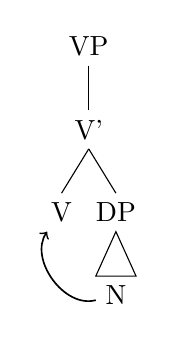
\begin{tikzpicture}
\Tree[.VP [.V' [. \node(subj3){V}; ] [.DP \edge[roof]; \node(subj2){N}; ] ] ]
\draw[semithick, <-] (subj3) to [bend right=70] (subj2);
    \end{tikzpicture}
\end{figure}

Without bringing systematically noun-incorporating languages into the discussion, such as the ones from the Iroquoian family \parencite{mithun2009polysynthesis}, Frisian, or West Greenlandic \parencite{Marti2015}, it is possible to find such behavior in now-lexicalized object-verb compounds in English too. I illustrate the case of \textit{to babysit} (also valid for \textit{to birdwatch, to fingerprint}, and other such compounds) in \reffig{babysit_tree}.

\begin{figure}[htb]
\caption{Portion of syntax tree illustrating the object-verb compound \textit{to babysit} in English as a result of noun incorporation.}
\labfig{babysit_tree}
    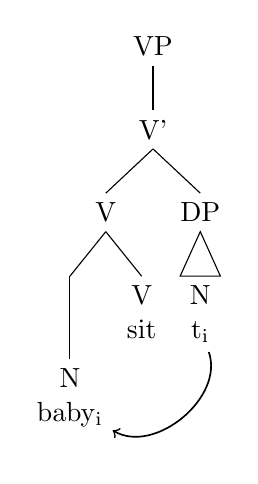
\begin{tikzpicture}
\Tree[.VP [.V' [.V [\node(subj3){N\\baby\textsubscript{i}};] [.V\\sit ] ] [.DP \edge[roof]; \node(subj2){N\\t\textsubscript{i}}; ] ] ]
\draw[semithick, <-] (subj3) to [bend right=70] (subj2);
    \end{tikzpicture}
\end{figure}

In \posscite{Marti2015} account, then, the only difference between indefinite null objects and incorporated nouns such as \textit{baby} in \textit{to babysit} would be that the former are phonologically null, while the latter are not. Noun incorporation gives rise to several effects, which \textcite[455-456]{Marti2015} reports based on evidence from West Greenlandic (an ergative language):
\begin{itemize}
    \item incorporated nouns must be bare, i.e. with no preceding article/determiner (just like indefinite null objects were shown to be "weak indefinites" in \refsec{whichobjects});
    \item the subject of a noun-incorporating verb is marked with absolutive case like the subjects of intransitive (unergative) verbs and the objects of transitive verbs, while the subjects of transitive verbs are marked with ergative case (mirroring the intransitive behavior of object-dropping transitive verbs);
    \item incorporated nouns always precede the verb in the linear word order, regardless of the position a full-fledged direct object would take in the sentence;
    \item incorporated nouns are interpreted indefinitely and non-specifically (just like indefinite null objects);
    \item incorporated nouns take narrow scope with respect to other operators in the sentence (as argued about indefinite null objects in \refsec{whichobjects});
    \item verbs undergoing noun incorporation usually refer to "name-worthy, typical activities" (like indefinite null objects, as shown on \refpage{activityfocus});
    \item verbs undergoing noun incorporation tend to have "conventionalized meanings", as noted before on \refpage{drinkingdrop} relatively to the imbibe-alcohol conventionalized meaning of the verb \textit{to drink} used intransitively.
\end{itemize}

\textcite[461-463]{Marti2015} then proceeds to test the hypothesis that verbs allowing indefinite object drop and verbs allowing noun incorporation share common properties with evidence from Frisian, a Germanic language having both indefinite null objects and noun incorporation. Her analysis demonstrates that transitive-made-intransitive verbs and incorporated-into verbs indeed belong to the same class. A crucial property both types of verbs share is, for instance, that only verbs selecting for a Patient object and having a volitional subject can participate in these constructions (making it only possible for verbs such as \textit{to notice, to hate, to know} in English to participate in \textit{definite}, not \textit{indefinite}, object drop).\\
Purely pragmatic accounts of indefinite implicit objects, as revealed on \refpage{activityfocus_end}, fail to take into account the cluster of properties shared by noun-incorporating and object-dropping verbs alike. On a side note, \textcite[249]{Mittwoch2005} comments on a construction sharing similar properties with noun incorporation, i.e. the \textit{out}-verb formation (e.g. \textit{I don't think they can outbuild us)}, which is a productive process where the original object gets omitted to put the focus on the activity\sidenote{In particular, on a competitive perspective about the activity, which is typical of commercials.} and the "resulting form selects for an object that belongs to the same class as the subject" (typical of low-transitivity utterances, as per \textcite{HopperThompson1980}).


\paragraph{Affected Agents, effected Patients} 

I will now tackle an aspect of indefinite objecthood originating directly from the account of transitivity as a prototype concept by \textcite{HopperThompson1980} and later literature\sidenote{Refer back to \reftab{ht1980_parameters} and further considerations in \refsec{theory_transitivity}.}, i.e. the need for the subject and the object of transitive sentences to be maximally distinct in their semantic behavior. This requirement was formalized by \textcite[30]{Naess2007} in the Maximally Distinguished Arguments Hypothesis. This observation led some authors\sidenote{Refer back to \refsec{whichverbs}.} to posit change-of-state verbs such as \textit{to break} as obligatorily transitive, since they feature\sidenote{Ignoring uses where the subject is non-Agentive such as \textit{The ball broke the window} and anticausative uses such as \textit{The window broke}.} a volitional, unaffected Agent and a non-volitional, affected Patient. As argued time and again in this Chapter, indefinite object drop is far from being prototypical behavior for transitive verbs. Under this lens, then, it would make sense to find that indefinite null objects are more common with verbs having affected Agents (i.e. Agents being the endpoint of the event) and/or effected Patients (i.e. Patients brought into existence by the event the verb refers to). Such an analysis is discussed in detail in \textcite{Naess2007}.\\
\labpage{affectedagent}Let us consider affected Agents first. \textcite[158]{tenny1994aspectual} calls them "measuring arguments", in that they delimit the event "by undergoing a change of state that marks the temporal end of the event". For instance, the event described by \textit{John ate} would be delimited by the affectedness of the Agent (in this case, the feeling of fullness), rather than by the affectedness of the unmentioned Patient. On the opposite, if one wanted to focus on the affectedness of the Patient, they would then have to resort to a transitive use of the verb \textit{to eat} \parencite[80]{Naess2007}. An affected-Agent interpretation of intransitive \textit{to eat}\sidenote{Such an account was first offered, \textit{in nuce}, in \textcite{Wierzbicka1982, starosta1978valence, nedjalkov1988typology, haspelmath1994passive}.}, which may or may not convince the reader yet by means of this example in English, becomes quite more persuasive in the account by \textcite[61-63]{Naess2007} of the same verb in Yucatec, a Mayan language spoken in the Yucatán Peninsula. In this language, due to its Agent being affected, \textit{to eat} patterns aspectually and morphologically with change-of-state verbs, not with activity verbs (as one would expect). Crosslinguistically \parencite[126]{Naess2007}, ingestive verbs (\textit{to eat}, \textit{to drink}, but also \textit{to learn}) consistently show characteristics typically belonging to intransitive verbs \parencite{Amberber2009, Amberber1996}, leading \textcite{marantz1981nature} and subsequent decades of literature on indefinite object drop to consider them "class representatives" of the typical behavior of verbs allowing for indefinite object drop. Taking the affected-Agent interpretation to the extreme, in some languages (such as Korean and Turkish) \textit{to eat} is even used as a grammaticalized marker of Agent affectedness, e.g. as an auxiliary, as a light verb, in constructions where it expresses undergoing or adversativity \parencite[75]{Naess2007}, and in antipassive constructions\sidenote{Used in ergative languages to convey certain aspectual and modal nuances. They are called "antipassives" because, much like in passive sentences the object of the active sentence becomes the subject and the subject of the active sentence is deleted, in antipassive constructions the object is (usually) deleted and the subject changes case from ergative to absolutive case.} \parencite[414]{Naess2011}. \labpage{antipassives} \textcite{Nicolas2019} offers an interesting account of the features null objects in English share with antipassive constructions. Moreover, an affected-Agent account can be easily employed to explain linguistic behavior that would otherwise remain unmotivated, such as the resistance of the verb \textit{to lock} to object drop as opposed to the ease one finds in using \textit{to eat} without an overt object, as noted by \textcite[30]{PethoKardos2006}. They argue that the opposite behavior of these two verbs with respect to indefinite object drop "does not become clear", on the basis of their selection restrictions\sidenote{More on selectional restrictions and object recoverability in \refsec{recoverability}.} having comparable extent (i.e. the objects of \textit{to eat} are edible items, the objects of \textit{to lock} are items provided with a lock). The reason for this difference, however, becomes quite clear when one considers that the subject of \textit{to eat} is an affected Agent, while this does not hold true for \textit{to lock}. However, it should be noted that while this analysis works, allegedly, for English, it is not universally valid for other languages. For instance, \textit{chiudere (a chiave)}, the Italian equivalent of English \textit{to lock}, can also be used intransitively, at least in spoken language (e.g. \textit{Hai chiuso?} 'Did you lock?', asked to someone leaving their house). \textcite{Isingoma2020} observes that object drop is also possible with \textit{-siba}, the equivalent of English \textit{to lock} in Rutooro\sidenote{A language of the Bantu family, spoken in western Uganda.}. Thus, Agent affectedness is a relevant facilitator of object drop, but its role has to be put in perspective (refer also to \refsec{agentaffect} for more considerations on this).\\
It is also important to note that while Agent affectedness is inherent to the semantics of some verbs (such as ingestion verbs), it may also be activated by verb-external elements of a clause. Let us consider the example sentence \textit{John murdered for the money} \parencite[136]{Naess2007}. In this case, the affected-Agent interpretation is fostered by the purpose clause \textit{for the money}, since the Agent's motive for the homicide is a direct gain, i.e. something that positively affects the Agent. Finally, the affected-Agent account can also explain constructions of the type \textit{have a drink, have a lick, have a bite} \parencite[758, 771]{Wierzbicka1982}. The author argues that in such constructions, \textit{have} has a detransitivizing function in that it backgrounds the object while focusing on the Agent. Not only that, but also, \textit{have a [verb]} events deviate from the transitive prototype because their Agent is affected by it (typically, by enjoying the activity the verb refers to), while the Patient is minimally affected.\\
Let us now discuss the other kind of argument deviating from the transitive prototype, i.e. effected Patients. These are non-affected objects that come into existence thanks to the very action described by the verb, and only if this action is brought to completion, e.g. the letter in \textit{John is writing a letter} or the cake in \textit{John is baking a cake}. Such constructions tend to feature indefinite null objects crosslinguistically and to have unaffected Agents, making it necessary to provide a different analysis than before in this Section \parencite[127-128]{Naess2007}. What affected-Agent and effected-Patient constructions have in common is that they both show low semantic distinctness between Agent and Patient (making them the optimal environment for felicitous indefinite object drop, based on \textcite{HopperThompson1980}), and they both largely depend on the semantics of the verb itself. As \textcite[127]{Naess2007} and \textcite[421]{Naess2011} observe, the low-distinctness of effected Patients is so embedded in the verb semantics that the very intransitive use of an effected-Patient verb evokes the non-referentiality of the object. This is most evident in imperfective contexts\sidenote{I will come back to the role of (im)perfectivity as a factor determining indefinite object drop in \refsec{perfectivity}.} (e.g. \textit{John was writing}), where the effected Patient is not presented as fully effected yet, and thus it is even less prominent in the discourse. On the contrary, perfective contexts tend to block indefinite object drop with effected-Patient verbs (e.g. \textit{? John had written}), while the same does not usually hold for affected-Agent verbs (e.g. \textit{John had eaten}). Crucially, an effected-Patient account can be used to explain why, as first observed by \textcite[96]{Fillmore1986}, intransitive \textit{to bake} in English (e.g. \textit{I spent the afternoon baking}) can only be understood to refer to the act of baking "bread or pastries, but not potatoes or ham". \textcite[135]{Naess2007} easily explains this linguistic fact by observing that the bread-or-pastries interpretation features an effected Patient, while the potatoes-or-ham interpretation features an \textit{affected} Patient, which makes the verb prototypically transitive and, thus, resistant to indefinite object drop. On the same note, intransitive \textit{to paint} (e.g. \textit{He paints}) is interpreted to refer to the act or habit of painting pictures, not house walls.


\section{A working definition of "indefinite object drop"} \labsec{theory_workingdef}

This dissertation is about indefinite null objects, whose nature I discussed throughout this Chapter with reference to traditional and recent literature alike. It is time to end this Chapter with some more detail on what this thesis is going to focus on, and also on what is going to be ignored in my experimental account of indefinite object drop.\\
As I mentioned in \refsec{theory_continuous}, I assume there is a distinction between \textit{indefinite} object drop, motivated by linguistic factors (see \refch{factors} and \refch{predictors}) of varying nature, and other kinds of object drop, such as definite null objects depending on Topic drop, genre-based null objects, and implicit objects depending on extra-linguistic context. This choice is motivated by lexical, semantic, and pragmatic accounts of the indefinite object drop discussed in this Chapter. Crucially, while I assume that verbs participating in the indefinite object drop construction show two surface sentence structures while being single lexical entries (\refsec{theory_entries}), I will not take a stance with respect to the problem of whether indefinite and definite object drop form part of a continuum or are two discrete, binary phenomena (\refsec{theory_def_vs_indef}). Indeed, one could interpret the distinction between the different kinds of object drop as stemming from a situation like the one in \reffig{objectdrop_venndiagram}, where virtually any verb can participate in object-dropping constructions, but in different ways depending on the underlying factor.

\begin{figure}[htb]
\caption{A concentric view of the factors determining the possible continuum between definite and indefinite object drop.}
\labfig{objectdrop_venndiagram}
    \begin{tikzpicture}
\coordinate (O) at (0,0);
\foreach \j in {1,...,3} \draw (O) circle (3.5-\j);
\foreach \k/\text in {0/extra-linguistic context,1/intra-linguistic context,2/semantics} \draw[decoration={text along path,reverse path,text align={align=center},text={\text}},decorate] (2.6-\k,0) arc (0:180:2.6-\k);
    \end{tikzpicture}
\end{figure}

Let us interpret the examples in \ref{concentric} in the light of \reffig{objectdrop_venndiagram}. In \ref{concentric1}, the referent of the omitted object (gas) is supplied by pragmatics \textemdash if one wanted to echo \textcite{Glass2020}, it is recoverable because in the sub-community of car-drivers it is customary to say cars "drink" to refer to them burning fuel. In \ref{concentric2}, the definite null object is immediately recoverable from the linguistic context provided in the sentence, and no additional extra-linguistic context is needed to interpret this utterance. Instead, the indefinite null object in \ref{concentric3} is interpretable with no context whatsoever, given that the semantics of the verb (and of the Agent, as argued on \refpage{affectedagent}) are sufficient for its recoverability.

\ex. \label{concentric} \a. \label{concentric1} It drinks $\varnothing$ a lot! \\ (in the social context of someone speaking about a car)
\b. \label{concentric2} \# My milk has been opened, who drank $\varnothing$?
\c. \label{concentric3} He drinks $\varnothing$.

One could, naturally, have qualms with respect to the full grammaticality of \ref{concentric2}, since English, after all, is not typically a language allowing definite null objects outside genre-specific environments. Moreover, one may want to keep verb-specific semantic affairs separate from extra- and intra-linguistic contextual information. In this case, the concentric, continuous view depicted in \reffig{objectdrop_venndiagram} would not correspond anymore to the theory, and one would have to adopt a strictly binary definite-or-indefinite perspective. Such an account easily handles cases where the same verb can appear in indefinite object drop constructions when proper situational context is provided, but not in zero-context environments, as in \ref{bindrop}.

\ex. \label{bindrop} \a. \label{bindrop1} Do you even lift $\varnothing$, bro? \hfill \parencite[9]{Glass2020} \\ (common among people training for strength in gyms)
\b. \label{bindrop2} *John had lifted $\varnothing$.

What is important, here, is that the same factors acting on no-context indefinite null objects are also active in context-rich scenarios, regardless of the continuous or binary view one adopts. What matters is that additional context (such as the one granted by a sub-genre) makes it possible for a verb to license indefinite implicit objects more freely than in no-context utterances. Thus, by studying the factors determining indefinite object drop in no-context utterances, I am still providing useful information to understand context-depending object drops, although without committing to a specific interpretation of the distinction between indefinite implicit objects and other null objects.\\
To sum up, my stance is that:
\begin{itemize}
    \item it is possible to characterize \textit{indefinite} null objects, whether they form part of a continuum having definite null objects at the other end or not (e.g. in a binary account of this distinction), as discussed in \refsec{theory_def_vs_indef};
    \item indefinite object drop is possible both with change-of-state verbs and with incremental-theme verbs (refer to \refsec{whichverbs}), to different extent, and the understood omitted object is not \textit{something} but the most prototypical Patient for a given verb sense in a given context (refer to \refsec{whichobjects});
    \item rather than positing two separate lexical entries for the overt-object and null-object uses of a transitive verb allowing indefinite object drop, a better account would have a single entry in the lexicon for the verb, which would then admit a null object under specific circumstances (refer to \refsec{theory_entries});
    \item the same semantic and aspectual factors allowing for indefinite object drop in no-context utterances are active in context-rich utterances, where context can be provided by linguistic means or via community-specific world knowledge (refer to \refsec{theory_workingdef}).
\end{itemize}

I will explore the main semantic, aspectual, and pragmatic factors playing a role in indefinite object drop in \refch{factors}.
\setchapterpreamble[u]{\margintoc}
\chapter{Indefinite implicit objects}
\labch{indefinitedrop}

pare che ormai questo capitolo non serva più (?)
% \setchapterimage[6.5cm]{seaside}
\setchapterpreamble[u]{\margintoc}
\chapter{Factors allowing indefinite object drop}
\labch{factors}

In \nrefch{objectdrop} I presented indefinite object drop as a marked construction deviating from the transitive prototype. Indefinite object drop has been argued to be binarily distinct from definite object drop, to be possible with some or all transitive verbs, to imply an unsaid \textit{something} or a prototypical object different for each verb, to make the verbs participating in this construction have an additional, intransitive entry in the lexicon or just the transitive one. Several answers were proposed to these conundrums in the literature, and I provided my own perspective.\\
In this Chapter, I am going to focus on the main intra-linguistic (semantic, aspectual, and pragmatic) factors allowing a transitive verb to participate in the indefinite object drop construction, based on literature on this topic. I will return to the subject of recoverability, manner specification, telicity, perfectivity, and iterativity in \nrefch{predictors}, where I will define them as predictors of indefinite object drop in my Stochastic Optimality Theoretic model.


\section{Semantic factors} \labsec{semanticfactors}

\subsection{Recoverability} \labsec{recoverability}

\paragraph{An intuitive notion of recoverability}

As observed several times in \refch{objectdrop}, recoverability is the \textit{sine qua non} of object omission. \textcite{Cote1996} even went as far as to identify it as "the only absolute constraint on null arguments". Intuitively, this notion can be used to tell apart definite implicit objects (whose meaning is recoverable from context, be it extra- or intra-linguistic) and indefinite implicit objects (whose meaning is recoverable from the semantics of the verb itself). Even authors who cautiously \parencite{Resnik1993, Resnik1996, OlsenResnik1997} or openly \parencite{Glass2013, Glass2020, glass2022english} reject a distinction between definite and indefinite object drop still maintain a certain notion of recoverability as a fundamental requirement for object drop. Let us discuss this in some more detail.\\
Decades of literature on the matter teem with pre-theoretical definitions of object recoverability. The oldest is in \textcite[105]{Ohlander1943}, where the author argues that object-less utterances "may appear complete enough" by virtue of the fact that "the element to be understood or supplied is so self-evident that the gap is mentally filled in by the audience more or less unreflectingly". Like many others, Ohlander makes reference to the notion of recoverability without using this exact wording. Similarly, \textcite{HickmanEtAl2016} resort to the idea of "conceptual defaultness", i.e. the property of unmentioned direct objects whose omission does not depend on an informational failure on the part of the speaker/writer \textemdash on the contrary, defaults are omitted to comply with the Gricean maxim of quantity, since their very mention "would be unnecessary and, perhaps, awkward" \parencite[516]{HickmanEtAl2016}.\\
Interestingly, recoverability appears to be such an intuitive notion as to become a major determinant of argument omission (not limited to indefinite object drop) in the early stage of grammar acquisition crosslinguistically, even in context and languages where adult grammar would normally prohibit it \parencite{allen2000discourse, RatitamkulEtAl2004, Medina2007, sopata2016null, Rasetti2003, PerezLerouxEtAl2011, PerezLerouxEtAl2013, Perez-LerouxEtAl2018, OGradyEtAl2008, Ingham1993}. Young children are shown to omit objects (and other arguments) of verbs they are exposed to, both in transitive and intransitive utterances, if extra-linguistic context makes them sufficiently recoverable.


\paragraph{Between lexical and contextual recoverability}

In \textcite[7]{Kardos2010}'s words, omitted objects are recoverable "either through lexical stereotypes or based on the context". In a sense, it is not even necessary to postulate a binary distinction between the two facilitators of recoverability, since "lexical stereotypes" (i.e. the selectional preferences of a verb) descend from world knowledge, situational context is where meaningful conversations happen, and narrower context enables more object omissions without contradicting world knowledge (more on this in \refch{objectdrop}, and in \textcite{Glass2013, Glass2020, glass2022english}, where recoverability is intended as a matter of degree). A prime example of this is \ref{berghplay}, taken by \textcite[24]{BerghOhlander2016}, whose full interpretation depends on additional context. Indeed, this sentence in isolation has no single interpretation. \textit{What} did they play beautifully? Was it an instrument or a game? And what kind, exactly? However, while context would make it possible to know the referent of this indefinite implicit object, the semantics of the verb (in particular, its selectional restrictions) still provide us relevant information without the need for additional context. Indeed, we know that they played either a game or a musical instrument. This would not be possible, for instance, with a selectionally un-restricted (or, better, very loosely restricted) verb such as \textit{to make}.

\ex. \label{berghplay} They played beautifully.

This also holds true for verbs with much stricter selectional preferences than \textit{to play}, e.g. the verb \textit{to eat}, to which I devoted some pages in \refch{objectdrop}. As noted by \textcite[149]{Cote1996} among others, intransitive \textit{to eat} tends to refer to a meal (which is the prototypical item humans eat), but it does not have to. In context-rich utterances, the actual referent may be different, depending on "the underlying context and intentional structure of the discourse structure at the time of utterance". Crucially, context may make it obvious that the omitted Patient is some specific kind of edible item (e.g. pasta, hamburgers, or even something as extravagant as Hawaiian pizza), but it cannot make it deviate from the basic selectional preferences of the verb\sidenote{Unless, of course, the verb takes a specialized meaning in a specific sub-genre, e.g. \textit{to eat} in a game of chess would mean \textit{to capture enemy pawns}.} \textemdash the omitted Patient has to be something edible.\\
Semantically-licensed recoverability also interacts with world knowledge, specifically with societal norms, in \textcite{Goldberg2005}. In this case, the author argues that politeness is a driving factor in the omission of direct objects occurring with verbs of bodily emission, since they are very imageable (hence, recoverable), but also very taboo in usual social contexts. On the other hand, it would be easy to imagine that in contexts where such verbs are not taboo (i.e. in medical literature, or among \textit{aficionados} of certain sexual kinks) the main driver of object omission would be contextual inferability, rather than misguided concerns for politeness. Either way, context and world knowledge (about the verb itself, but also about proper customs) comply with verbal semantics.\\
Consistently with all the previous observations on recoverability, \textcite{Mittwoch2005} and \textcite{Glass2013} also observe that the referent of indefinite implicit objects corresponds to the literal meaning of the verb, rather than to metaphorical or idiomatic meanings. For instance, intransitive \textit{to read} refers to "written or printed material rather than, say, the stars or coffee grounds" \parencite[2]{Mittwoch2005}. Likewise, when a verb has strict selectional preferences (e.g. \textit{to eat} selects for edible items) and one of its near-synonyms has broader preferences\sidenote{An in-depth discussion of such verb pairs will be tackled in \refsec{mannerspec}.} (e.g. \textit{to devour} selects for edibles, but also for metaphorical items such as books), direct objects are much more likely to be dropped with the former than with the latter \parencite[5]{Glass2013}. Clearly, this mechanism is in place to maximize recoverability, since the literal selectional preferences of a verb are known and predictable (based on lexical semantics and world knowledge), while its metaphorical or idiomatic behavior is largely arbitrary and unpredictable. More in general, the more an object is semantically dependent from a verb, the more likely it is to be omitted \parencite[203-204]{Rice1988}.


\paragraph{Semantic selectivity as a proxy to recoverability}

Let us now look in more detail into semantic selectivity as the main verb-internal, context-independent factor allowing for object recoverability. So far in this Section, I made the case that knowing the specific type of objects a verb favors in its selectional preferences is the first step towards object recoverability and, thus, felicitous object omission. World knowledge and context shape the way we process object-less transitive verbs when accessing their selectional preferences. However, as hinted before, there is a close correlation between indefinite object drop and the breadth of a given verb's selectional preferences, regardless of the actual items or family of items it tends to occur with \parencite{Garcia-VelascoMunoz2002, Liu2008, Glass2020, Medina2007, MaoueneEtAl2011, OlsenResnik1997, Resnik1993, Resnik1996}.\\
testo

% *Garcia-Velasco & Munoz (2002: 4)*  
% > Omitted objects are generally restricted to complements with a low degree of semantic independence from % the verb. There are many verbs whose omitted objects are clearly understood because they are inferred  from a % very narrow, if not exclusive, range of possibilities. % According to the author, this explains the differences observed among semantically related % verbs.

% *Liu (2008: 302)*
% > An important reason that the transitive-turned intransitive verbs focusing on activity can be used in
% such a way while object-deleting verbs cannot is that the possible objects of the former
% type of verbs are very transparent in the Encyclopedia but those of the latter are
% not. For example, whenever we say someone is reading, it must mean the reading of
% something readable among a very few choices, such as a book, a newspaper, or a
% magazine; by contrast, there is no such transparent information in the Encyclopedia
% about what a person can know. There are simply too many different types of information
% that a person can know. The transparent meaning of the transitive-converted
% intransitive verbs makes the activity reading of these verbs possible.

% *Glass (2020: 3)*
% > Selection is the idea that transitive verbs provide information about the nature of the referents of the objects they combine with

% *Glass (2020: 4)*
% >  It is often claimed that a verb’sobject can only be omitted if the object’s identity can be ‘recovered’ (an idea which dates back to Jespersen 1927:  volume II3; Lehrer 1970, Rice 1988, Cote 1996).  Resnik’s finding – thatverbs facilitate omission when they provide more selectional information to recover the omittedobject – substantiates that claim. Moreover, Hopper & Thompson 1980 group together morpho-syntactic and semantic features that they associate with high and low ‘transitivity’, viewed asa gradient property of clauses.  For them, the most ‘transitive’ clauses involve objects whichare informationally distinct from the verb, while less-transitive clauses involve informationallyunsurprising  objects.   Resnik  builds  on  that  observation  by  showing  that  object  omission  –associated with lower transitivity – is favored for objects that are easily inferred

% *Medina (2007: 17)*
% > One factor that has been shown to be relevant to the implicit object construction is that of the semantic narrowness of the verb’s meaning or selection of arguments.  Rice(1988)pointed out that implicit objects tend to be typical in some way of the verb and that verbs which occur with a broad range of objects (and thus no object is particularly typical) tend to resist implicit objects.  Similarly, Levin(1993)identifieda set of verbs which participate in the "unspecified object alternation" and she noted that for these verbs, the object is generally understood as being a typical object of the verb.  Goldberg(2005, Draft)also cites recoverability as a necessary (but not sufficient) condition on the possibility of a verb being used in what she terms the “Implicit Theme Construction”

% *Medina (2007: 178)*
% OS è la misura sperimentale di Medina che somiglia alla mia distribuzionale!
% > an implicit object of a high OS verb should be more recoverable since the verb occurred with objects that are highly similar to one another

% *Garcia-Velasco & Munoz (2002: 11)*  
% PRINCIPLE OF RELEVANCE!!!  
% > However, it is obvious that not all verbs admit this process. If the focus in an activity
% is the verbal action itself, rather than the result or effect upon the participants, those verbs
% whose objects are drawn from a restricted range of possibilities will be likely candidates to
% take understood objects.
% Thus, some authors (Lehrer 1970; Fellbaum & Kegl 1989) have suggested a sort of
% scale or degree of specificity of verbal objects. At one pole of the scale we would have the so-
% called “cognate” objects, so specific and predictable that they do not usually appear in
% linguistic expressions (see footnote 4). Examples of verbs taking them include: sing, dream,
% live, die, laugh, dance. Cognate objects are believed to coincide with the selection restrictions
% on the object position, which makes them redundant if present in the actual expression. If the
% object appears as a sort of selection restriction it need not be recovered in the context since it
% is already available from the verb’s semantics. Groefsema (1995: 152) formalises this idea
% with Jackendoff’s system of representation and proposes the following principle:  
% << an argument can be left implicit if the verb puts a selection restriction on the argument such that it gives us an
% interpretation in accordance with the principle of relevance. >>  
% Basically, the principle of relevance claims that expressions show optimal relevance when
% they enable the speaker to derive an adequate number of contextual effects for no unjustifiable
% processing effort.  
% A second group of verbs take their objects from a very limited range of potential
% candidates, and, therefore, can be easily retrieved if omitted. Examples include: read, write,
% clean, eat. Lehrer (1970) adds the following: sew (cloth, clothes); spill (liquid, collection of
% small pieces of some physical object, etc.); spend (time, money, energy), among many others.
% Our second hypothesis, then, can be formulated as follows:  
% Hypothesis 2  
% The more predictable an object is (given the meaning of the verb), the more likely it will be to
% be left out.

% *Maouene et al. (2011: 1)*
% >  ‘Light’ verbs, such as do, make, get, take, and go are more abstract and label a wide range of
% specific events that have little in common, other than the relation itself. ‘Heavy’ verbs, such
% as kick, eat, drink, and read seem more concrete and specific and may refer to a smaller
% range of events, often ones that involve narrow classes of actions and objects

% *Olsen & Resnik (1997: 4-5)*  
% > Verb-object individuation is, therefore, another way of describing the selectional
% relationship between the verb and the object. Selection restrictions have
% traditionally been construed as semantic information carried by the verb about its
% arguments, both in their role as constraints (e.g. *Eli drank cookies) and as
% features transferred to underspecified arguments (e.g. Eli drank it implying that it
% is [+ LIQUID]. Resnik's (1996) theory, going beyond simple Boolean features,
% makes it possible to place selectional relationships on a continuum—that is, to say
% why drank a drink is intuitively a "better" verb-object combination than drank
% kerosene, which is in turn better than Eli drank cookies. This is done, in sum, by
% formalizing in quantitative (probabilistic) terms the extent to which the verb
% predicts the conceptual type of its argument, using a quantitative measure based
% on "information" in the sense of Shannon (1949). The measure assigns the ratings
% in (11), for example. (See Resnik 1996 for more details.)  
% (11) Eli drank some wine [7.65] / kerosene [5.61] / sincerity [0.00].  
% To phrase this in terms of H&T's continuum, the more strongly a verb
% selects its object, the more information about the object is carried by the verb
% itself, and thus the less individuated the object is from the verb. A very strongly
% selected object such as tune in Eli sang a tune, carries relatively little new
% semantic information. It is therefore less individuated from the verb. In the same
% sense a reflexive object in a sentence like Eli shaved himself carries little new
% information about an agent and is therefore less individuated from it.  
% The cognate object construction is at the low transitivity end of the
% individuation spectrum; as in (12), otherwise intransitive verbs usually take
% objects that are morphologically and semantically related to the verb (see
% Macfarland 1995 and references therein). Consistent with the transitivity
% hypothesis, low object individuation correlates with other low transitivity
% properties; as Rice (1988:207–208) notes, for example, the verbs participating in
% cognate object constructions generally refer to "predications that are considered to
% be intransitive" and "in many languages the verb is treated lexically and
% syntactically as intransitive."  
% (12)a. Benjamin laughed a silly laugh/*a silly chuckle.4  
% b. Benjamin smiled his winning smile/*his winning grin.  
% Indeed, some have claimed that cognate object constructions are licensed only if
% the object is modified, so that it is more individuated from the verb. 

% *Olsen & Resnik (1997: 6)*  
% > Turning to implicit object constructions, if we have appropriately extended
% the individuation feature of the transitivity hypothesis with respect to selectional
% constraints, we would again expect a lesser degree of object individuation (one
% facet of which is stronger selectional constraints) to correlate with a lesser degree
% of transitivity on other dimensions. Indeed, this is the case. In a study applying the
% quantitative theory of selectional constraints (replicated using a corpus of text, a
% corpus of transcribed speech, and human subject norms as sources for the
% probability estimates required by the theory), Resnik (1996:148) found that
% "[transitive] verbs participating on one of the implicit object alternations have a
% significantly higher strength of selectional preference for the direct object than
% verbs that do not." [...]  
%  Moreover, although some strongly selecting verbs fail to
% appear with implicit objects (apparently owing to their aspectual properties), the
% converse is never true; Resnik (1993:88) therefore concludes that "strong
% selection is a necessary condition for object omission."




\subsection{Agent affectedness} \labsec{agentaffect}

ne parlo nel capitolo teorico generale: spostare qui o fare soltanto riferimento?

\subsection{Manner specification} \labsec{mannerspec}

qui devo dire che "manner" è un termine molto ambiguo, perché io la intendo nel senso tecnico di "manner specification" eat/devour, ma altri lo usano in opposizione a "result" per indicare, sostanzialmente, activity vs accomplishment/achievement

% # Manner/Result distinction and manner specification

% *Naess (2007: 130-134)*  
% (Rice 1988 :203). She argues that objects can be omitted when there is a
% default interpretation for a missing object, exemplifying this with ‘John ate a meal’
% as the default interpretation for John ate. The verbs allowing such omission must
% be “semantically neutral”, not conflating action and manner (contrast John ate with
% *John nibbled), and the omitted object shows a “low degree of semantic independ-
% ence from the verb” (Rice 1988 :204).

% *Naess (2007: 139)*  
% SI RICOLLEGA AL DISCORSO DELL'AFFECTED-AGENT / EFFECTED-OBJECT  
% > One general restriction appears to be that IOD does not occur with verbs
% whose semantics includes elements which refer specifically to the manner in which
% the patient is affected. This explains the difference noted by Rice between what she
% calls a “semantically neutral” verb like eat, which omits its object without difficulty,
% and “action-plus-manner” verbs like munch or nibble. The difference between
% these two types of verbs is that the additional semantic features present with munch
% and nibble pertain to the specific effect of the action on the patient rather than the
% agent, and so these verbs do not function primarily as affected-agent verbs and
% therefore do not normally omit their objects. However, if it is possible to construe
% the meaning element in question as pertaining to the effect on the agent – that is,
% where the manner in which the action was performed is seen as having some kind
% of influence on the effect achieved on the agent – object omission is in fact possi-
% ble: The dinner was delicious, but Jane had no appetite and only nibbled.  
% A related restriction obtains with verbs which describe actions whose precise
% effects depend on the nature of their patients. Goldberg (2001) suggests that a verb
% like break generally does not omit its object because different things “break in very
% different ways and with very different consequences” (p. 512). That is, the precise
% nature of an event such as breaking depends on what is being broken, and the pa-
% tient must therefore be specified, as it “supplies much of the relevant information”
% (Goldberg 2001 :512). Similarly, effected-object verbs such as build or make de-
% scribe actions whose execution depends on the kind of object produced – building
% is a different process when what is being built is a skyscraper than when it is a
% treehouse or a sandcastle, and there is no generalised process of “making” inde-
% pendent of what is being made.


% *Lorenzetti (2008: 65)*  
% FONDAMENTALE!!! AGGIUNGERE A PARAGRAFO SU MANNER SPECIFICATION  
% > Object omission has been frequently related to verb classes and to their semantic structure
% [Levin1993; Rappaport Hovav and Levin 1998]. Fellbaum and Kegl [1989], who put forward
% an analysis of understood objects on the basis of taxonomies, suggested that the semantic
% variability of a verb like eat, which allows both a transitive and an intransitive construction, is
% semantically motivated and can be explained by looking at the position of the verb in a
% taxonomic hierarchy. By taking a look at the verb troponyms57, they noticed that verbs such as
% nibble and dine are differently related to eat, in that the former represents a manner of eating,
% while the latter does not strictly refer to a manner, but rather to eating a substantial quantity of
% food at a certain time of the day.  
% This led them to posit two different semantic entries for eat, where eat1 is equivalent in
% meaning to eating a meal and behaves as if it had incorporated its cognate object; whereas
% eat2 is equivalent to ingest food in some manner. English possesses a number of verbs to
% indicate different kinds of meals, where the hyponym meal has been conflated with the verb,
% thus yielding to breakfast, to dine, to picnic etc. All of these verbs are intransitive, because
% they are specific lexicalisations of eat1. Other intransitive troponyms of the verb are mush,
% nosh and graze. They are not conflations of eat1 and the noun meal, but they are related to the
% verb, in that they refer to informal ways of eating a meal. By contrast, transitive eat2 has the
% sense of ingest food in some manner, and all its troponyms refer to a specific manner of
% eating, e.g. gobble, gulp, devour. Syntactically, they argue, the manner expression is a
% prepositional phrase adjunct, which always requires the presence of a direct object at the level
% of the surface structure, which is why these verbs necessarily require direct objects.
% The same situation is alleged to occur with drink, wash, draw and other related verbs. A
% corollary to this hypothesis is that omitted objects tend to belong to semantically neutral verbs
% as opposed to those which include a manner component. [...]  
% [57
%  Troponymy (from the Greek tropos, manner or fashion) defines a manner relation among verbs. Fellbaum and
% Miller, outlining the semantic network of English verbs called Wordnet, recognised that the identification of verb
% hyponyms is different from that of nouns, as exemplified by the fact that the "kind of" relation is not easily
% importable to the domain of verbs (cfr. A horse is a kind of animal is felicitous, but Mumbling is a kind of talking
% is not always so). Troponymy is a particular kind of entailment and can be expressed by the formula to V1 is to V2
% in some particular manner.]

% *Lorenzetti (2008: 66)*  
% > Rice [1988] contends that the manner component adds a certain degree of specificity,
% which makes the verb lose its basic status. The impossibility of omission may be then
% considered to be related to specific semantic components shared by verbal sets, which might
% foster or forbid omission. In addition to the manner component, a feature like completion can
% also make a verb incompatible with object omission. By contrast, the duration component is
% frequently associated to object omission.

% *Onozuka (2007: 539)*
% > Rappaport Hovav and Levin (1998) argue that the distinction between manner verbs
% and result verbs is crucial in accounting for the difference in elasticity, which these two
% types of verbs exhibit with respect to the variation of the argument structure. In short,
% their point is that manner verbs are quite flexible and can take part in various construc-
% tions, while result verbs lack pliability and do not allow argument structure variation.
% One argument that Rappaport Hovav and Levin rest on is the possibility of object dele-
% tion. They give the following examples:  
% 1. a. Phil swept.  
% b. *Tracy broke.  
% The contrast in (1) shows that (transitive) manner verbs allow object deletion, but result
% verbs do not. 1 On the other hand, Goldberg (2001) argues against Rappaport and Levin’s
% claim and makes the convincing argument that this distinction is not essential and that
% result verbs or what she calls causative verbs behave more flexibly with respect to argu-
% ment variation. [The principle of Omission under Low Discourse Prominence.]

% *Rissman (2016: 428)*  
% > If instrumental verbs are result verbs, and the instrument is inferred pragmatically,
% then instrumental verbs should pattern with prototypical result verbs such as break
% on a wide range of diagnostics. In this paper, I tested this prediction focusing on
% the diagnostic of object deletion shown in (4):  
% (4)a.b.Cinderella scrubbed all night long.  
% *Cinderella broke all night long.  
% Beavers & Koontz-Garboden (2012) argue that this test diagnoses result: if a verb
% allows object deletion, as in (4a), then this verb does not encode a result. Rappaport-
% Hovav (2008) explains this contrast in terms of the scalar semantics of result verbs:
% if a verb specifies a scale, then the entity changing along the scale cannot be
% omitted. (4b) is infelicitous because break encodes a two-point scale where its
% direct object changes from a non-broken to a broken state.
% This linking hypothesis makes the prediction that instrumental verbs should be
% infelicitous in this construction, as they encode a scalar result. [...]  
% In my studies, I focused on a particular variant of object deletion, which I term
% the "x-and-x construction:"  
% (6)a.b.Cinderella scrubbed and scrubbed all night long.  
% *Cinderella broke and broke all night long.

% *Rissman (2016: 436)*  
% QUESTA CONSIDERAZIONE TORNA SPESSO NEI MIEI APPUNTI  
% > As discussed above, I propose that the x-and-x construction targets agentive
% meaning. In particular, this construction highlights an atelic event in which the
% agent repeatedly performs an action. Given this highlighting of the agent's action,
% the direct object may be deleted, if the verb encodes some type of action on the part
% of the agent.

% *Garcia-Velasco & Munoz (2002: 6)*  
% > Some scholars, especially Fellbaum & Kegl (1989), attempt to explain aspects of the
% phenomenon by relying on lexical networks or taxonomies, as they call them. Thus, in the
% case of the verb eat, they propose the existence of two entries associated with two different
% semantic networks which predict its behaviour. Eat1 is equivalent in meaning to eat a meal,
% and, in this sense, it behaves just like other verbs which also include in their lexical structures
% a particular meal: breakfast, lunch, dine, brunch, snack, picnic. All of them share the feature
% of having incorporated their cognate object. Thus, the relationship of eat1 with those verbs
% would be similar to that of to dance with to tango or to waltz.
% Eat2 is equivalent to ingest food in some manner, and hence shows a behaviour
% parallel to those verbs of “manner of eating” such as devour, gobble, gulp. It is this manner
% component that forces the presence of the object (see Rice 1988 above). The authors claim
% that the same situation occurs with drink, draw, wash and their related verbs. Omitted objects
% tend to belong to semantically neutral verbs (eat, drink, study, speak, etc.), as opposed to
% those which introduce a manner component in their semantic structure (bite, devour, sip,
% memorise, utter, etc.). Rice claims that the manner component adds a certain degree of
% specificity to the action, which makes the verb lose its basic status 4 . The correlation seems to
% be the following: if the verb incorporates an object, it will be basically intransitive (unless it
% shows up as a cognate or hyponym) 5; if it incorporates an adjunct, it will be transitive. Note
% that this also explains the absolutive use of the verb drink. Since it incorporates an object
% (alcohol), this use of the verb is basically intransitive.

% *Garcia-Velasco & Munoz (2002: 7)*  
% ESATTO! PROBLEMATIZZARE QUESTA COSA IN UN CAPITOLO A PARTE, USANDO I MATERIALI DI QUESTO NOTEBOOK
% >  although both Rice (1988) and Fellbaum & Kegl (1989) suggest that the presence of a
% manner component in ‘manner-of-eating’ verbs accounts for the impossibility of omitting the
% object, Rappaport & Levin (1998) observe that manner-of-action verbs, as opposed to result
% verbs, are much more flexible in the range of syntactic contexts in which they can figure,
% allowing object omission. In this sense, manner-of-ingesting verbs may be the exception to
% the rule.


% *Melchin (2019: 2)*  
% AGENT = MANNER (cfr. appunti simili per gli Strumenti!)  
% > One frequently-cited
% case (see e.g. Jackendoff 2002) is the contrast between eat and devour: eat allows its object
% to be dropped, while the near-synonym devour does not. While they clearly do not have the
% exact same meaning, they are alike in most ways that are relevant to argument structure:
% both are verbs of consumption, specifically consumption of food through the mouth, where
% the external argument is the Agent doing the consuming, and the internal argument is the
% thing being consumed. At first glance, the only real difference in meaning has to do with the
% manner of consumption, where devour requires that the eating be particularly vigorous and
% voracious, while eat does not specify how the eating takes place. This difference has more
% to do with the Agent of consumption, specifically the manner in which the Agent does so

% *Melchin (2019: 3)*  
% OSSERVAZIONI CROSSLINGUISTICHE  
% > many of the problematic
% cases show consistent patterns from one language to another (modulo language-specific rules
% on the realization of arguments). For instance, I show in Chapter 3 that the translation
% equivalents of eat and devour in French, Dutch, and Arabic all show the same contrast as
% English in terms of the optionality of the object.

% *Melchin (2019: 45)*  
% uffa, mi ha fregato l'intuizione  
% >  The difference is one of hyponymy; the set of events described by devour is a subset
% of that described by eat. 

% *Melchin (2019: 46)*  
% MANNER AND RESULT  
% > there is a crucial difference between eat and devour that determines whether or not
% UOA is available: eat specifies only a Manner of acting, while devour specifies both a Manner
% and a Result (in roughly the sense of Rappaport Hovav and Levin 2010), namely that the
% object must be completely consumed in an event of devouring (a difference noted by Smollett
% 2005 and Piñón 2008). I claim that Manner and Result, as components of verb meaning,
% have syntactic consequences for a certain set of verbs, constraining which arguments must be
% overtly present in the syntax

% *Melchin (2019: 47-48)*  
% CONTROESEMPIO ALLA MANNER SPECIFICITY
% > Jackendoff (2002, p. 134, fn. 15) explicitly argues that the differences between these verb
% classes is, in fact, essentially due to arbitrary lexical specifications of the verbs. He notes that
% it is tempting to argue that whether a verb’s object will be obligatory or optional depends
% on the specificity of the verb’s semantics, so that verbs with a narrow meaning (like devour)
% will require an object, while for verbs with a wider meaning (like eat), the object will be
% optional. Jackendoff counterexemplifies this claim with pairs of verbs like serve and give,
% where the former may drop its indirect object while the latter may not, despite the fact that
% serve seems like a more specific counterpart to give. Jackendoff also raises the examples of
% juggle (six balls) and flirt (with Kim), stating that these verbs have highly specific semantics
% yet may drop arguments

% *Melchin (2019: 51)*  
% (ATTENZIONE che per Melchin la "manner specification" è abbastanza diversa dalla versione naive!)  
% >  Part of the meaning of eat is that the event denoted is undertaken by
% an agentive causer. According to the theory that I develop below, this means that it is a
% Manner verb.  [...] I claim that if a verb expresses Manner, then its agentive subject must be overtly present
% in the syntax, while if a verb expresses Result, then the argument of which the result state
% is predicated must be present. 

% *Melchin (2019: 52)*  
% > there are dynamic verbs, like clean, which are specified for neither Manner and Result and
% therefore may express either. 

% *Melchin (2019: 59)*  
% > In this section I propose that argument omission is constrained by whether or not the predicate
% in question expresses Manner or Result, components of lexical meaning defined in terms of
% the relationships of the core arguments to the event denoted by the predicate. I borrow the
% terms “Manner” and “Result” from Rappaport Hovav and Levin (1998, 2005, 2010), though I
% define them in a somewhat different way than they are used in those papers. A verb that
% expresses Manner requires that its external argument be an Agent of the event; a verb that
% expresses Result requires that its internal argument undergo some scalar change resulting
% from the event. When a verb expresses Manner (i.e., it is a “Manner verb”), the agentive
% subject cannot be omitted or replaced in the sentence, and likewise, when a verb expresses
% Result (a “Result verb”), the object undergoing the scalar change must be overtly expressed

% *Melchin (2019: 62)*  
% > Manner and Result, as characterized by Rappaport Hovav and Levin, are not mutually
% exclusive in the event structures of sentences; this is demonstrated in (20), in which the
% matrix verb introduces the Manner, and the resultative PP or AP provides the Result. What
% they claim is that an individual verb root can only express one or the other [...]  Beavers and Koontz-Garboden
% (2012, 2017) have shown evidence of a group of verbs, including many manner-of-killing and
% manner-of-cooking verbs, that express both Manner and Result, contrary to the predictions of
% Rappaport Hovav and Levin; 

% *Melchin (2019: 63)*  
% MANNER = AGENT  
% >  I propose that the Manner component of verb meaning is an
% entailment that the event is brought about by a participant acting in a particular manner
% – that is, an entailment that there is an Agent in the event. This entailment is implicit in
% Rappaport Hovav and Levin’s event-schematic characterization of Manner, shown in (22)
% above, in which the Manner component modifies an ACT predicate; however, they do not
% explicitly link Manner to the Agent role. Furthermore, I propose that the entailed Agent
% must be realized, and may not be omitted. 
% The link between Manner and agentivity is made by Beavers and Koontz-Garboden (2012),
% who show that while non-Manner verbs, such as the Result verbs break and shatter, allow
% instruments and inanimate causers as subjects, Manner verbs like scrub and brush do not,

% *Melchin (2019: 64)*  
% > A similar observation is made by Reinhart (2002, 2010), who links the property of requiring
% an Agent to the causative-inchoative alternation. Specifically, she notes that verbs that
% require an Agent do not undergo this alternation, while verbs that do not require an Agent
% may do so.

% *Melchin (2019: 65)*  
% POSSIBLE TEST FOR MANNER-HOOD
% > Thus, Manner can be characterized as the requirement that there is an Agent, or a
% participant acting in a certain manner, in the event structure.  Furthermore, this Agent must
% be expressed as the external argument of the verb, and may not be omitted, as shown in (27),
% or replaced with a non-agentive external argument, as shown in (25). This allows a more
% precise and testable definition of Manner than that of Rappaport Hovav and Levin (2010) as
% non-scalar change; rather than involving a change that cannot be characterized as scalar, it
% involves entailments about the role one of the participants plays in the event, and is made
% testable by the fact that this participant must be expressed as the external argument.

% *Melchin (2019: 66)*  
% WHAT IS AN AGENT
% > extend the definition of agentive causation to include any case where the force
% causing the event is spontaneously generated by inherent properties of the causing entity itself,
% and sustained throughout the event. This notion is referred to by Folli and Harley (2008) as
% teleological capability. 

% *Melchin (2019: 66)*  
% RESULT = THEME = OVERT DOBJ
% >  a Result verb entails that the Theme argument undergoes a scalar change in its
% entirety. Furthermore, as with the Agent entailed by a Manner verb, this Theme must be
% realized as a syntactic argument of a verb, in this case the internal argument. 
% When I claim that the Theme must undergo a scalar change “in its entirety”, I do not
% mean that the change must reach some specified endpoint or that the event must be telic;
% instead, the change (to whatever extent it occurs) must affect the entire entity denoted by
% the Theme. 

% *Melchin (2019: 71)*  
% DEVOUR = MANNER+RESULT
% > Now that Manner and Result are characterized in terms of agentivity and themehood in
% the event, rather than scalar versus nonscalar change, one can raise the question of what the
% properties of a verb with both of these meaning components would be. The event described
% by such a verb would require an Agent to act in a certain manner to bring it about, and
% would result in a scalar change affecting another participant. Syntactically, such a verb would
% not allow the omission of either the external argument or the internal argument; both would
% need to be realized in a sentence containing the verb. Rappaport Hovav and Levin (2010)
% claim that no such verbs exist, and that Manner-Result Complementarity holds (which they
% explain using the Lexicalizaton Constraint). However, in the next section, I show that devour
% is just such a verb.

% *Melchin (2019: 75)*  
% >  eat can take a resultative XP predicated by a non-selected argument, while
% devour cannot,  
% (44)  John ate the restaurant out of business.  
% (45) #The lion devoured the zoo out of business.

% *Melchin (2019: 77)*  
% CONSEGUENZE GROSSE SULLA TELICITY!
% > Given the claim above that devour is a Result verb and eat is not, this predicts that
% an event of devouring must maximally affect the edible parts of the Theme, while events
% of eating do not necessarily maximally affect the relevant parts. The standard view in the
% literature (e.g., Verkuyl 1972, 1993; Tenny 1994; Jackendoff 1996; Krifka 1998) holds that
% this is not the case, and that incremental theme verbs uniformly require that a quantized or
% bounded object be maximally affected by the event – in present terms, that all incremental
% theme verbs, including both eat and devour, have the Result component. This means that if
% the Theme is quantized or bounded (in the sense discussed in Footnote 6) the event will be
% telic. However, Smollett (2005) challenges this view, claiming that sentences with incremental
% theme verbs such as eat and build may be atelic even if the Theme is quantized, though
% this reading may be difficult to access without some contextual support (see Piñón 2008 for
% further discussion of this claim).

% *Melchin (2019: 84)*  
% > Thus, while clean is not necessarily specified for
% either Manner or Result, it must take on one or the other meaning in a sentence.
% A possible alternative to treating clean as underspecified for Manner and Result is to
% analyze it as lexical ambiguity between a Manner clean and a Result clean. However, there
% is a conceptual advantage to the approach taken here. 

% *Melchin (2019: 86)*  
% FONDAMENTALE!!! TABELLA CON TYPOLOGY 2X2
% > verbs marked with a negative value for one of the features can still express that 
% component of meaning, but verbs marked positive must necessarily express that meaning.  
% Table 3.1: Typology of Manner and Result [...]  
%  the typology in Table 3.1 can be explained using two principles:
% (i) a transitive dynamic predicate must express at least either Manner or Result; (ii) some
% verbal roots, by virtue of their meaning, necessarily express Manner or Result, or both (i.e.,
% they require that their external argument be an Agent, and/or that their internal argument
% undergo scalar change). Principle (i) is likely a consequence of the nature of dynamicity;
% an event involving one or more participants is not dynamic if there is no participant acting
% agentively, or undergoing some change (or both). 19 Principle (ii) is a consequence of the lexical
% semantics of certain verbs; verbs specified for Manner or Result will satisfy (i) vacuously. 
% The [– Manner, – Result] verbs are simply those transitive verbs which do not satisfy (ii),
% but which must take on one or the other feature in order to appear in a dynamic sentence.

% *Melchin (2019: 87)*  
% > for ambiguous verbs ([– Manner, – Result]), in addition to clean, there is cut, as mentioned
% above and extensively discussed in Levin and Rappaport Hovav (2013, 2014). 

% *Melchin (2019: 89)*  
% > We have now seen that devour is not alone as a Manner-Result verb; it is joined by certain
% verbs of manner-of-killing. I have also shown here that the set of verbs that has been classified
% as “manner-of-killing” by Beavers and Koontz-Garboden (2012) and others cited therein is
% not a unified class,

% *Kardos (2010: 7-8)*  
% Based on similar evidence, Levin and Rappaport Hovav revised their theory in their 2004
% paper in the following way. On the one hand, they still bolster the view that events denoted by
% eat and sweep consist of two subevents, namely, the action carried out by the eater (or
% sweeper) on the one hand, and the gradual disappearance of the apple, or the gradual
% “becoming swept” of the room. On the other hand, however, they note a significant difference
% between this event structure and that of truly complex causative verbs. They posit that the two
% subevents of an eating or a sweeping event occur at the same time and cannot be clearly
% separated since, as they put it, they are temporally dependent on each other. Therefore, they
% refrain from calling these true complex events, claiming that this duality can be grasped only
% conceptually, which explains why these events are simple from a linguistic point of view. In
% particular, the fact that the object of these verbs can be dropped, and that non-subcategorized
% objects can combine with them (see section 2), is regarded as evidence for the “simple event”
% character of eat-type verbs.


\section{Aspectual factors} \labsec{aspectualfactors}

% *Dvorak (2017: 115)*  
% SPOSTARE IN TELICITY/PERFECTIVITY!  
% > The issue
% here is that once the verb is in the -ing form, describing an ongoing event, the postulated
% distinction between activities and accomplishments is overridden. This is confirmed by the
% fact that all progressivized process verbs behave like activities for the purpose of Dowty’s
% (1979) classical tests distinguishing accomplishments from activities.

% Medina 224, in nota
% Finally, and perhaps most importantly, children under three years have been shown to distribute
% imperfective / perfective aspect in accordance with telicity in both production and comprehension (Olsen et al., 1998; Wagner, 2001; Weist, 2002; Weist et al., 1984). Thus, rather than assessing the relationship
% between imperfective / perfective aspect and the use of implicit objects, what may actually be being
% % indirectly assessed is the relationship between telic / atelic aspect and implicit objects.

\subsection{Telicity} \labsec{telicity}

Contents

% *Newman & Rice (2006: 5-6)*  
% > Van Valin and LaPolla (1997:112) explicitly remark that
% “...eat is not inherently telic, unlike kill and break; hence it must be
% analyzed as an activity verb, with an active accomplishment use”. For
% them, the ‘activity verb’ use (He ate, He ate spaghetti for ten minutes) is
% the ‘basic’ meaning of EAT.

% *Naess (2007: 77)*  
% SPOSTARE IN CAPITOLO SU TELICITY! (CONTINUA DOPO, CREDO)  
% > Of the properties included in Hopper and Thompson’s list of Transitivity pa-
% rameters, the most obvious candidate for an explanation for the intransitive be-
% haviour of ‘eat’ verbs would appear to be parameter C, “aspect” – telic vs. atelic. As
% Hopper and Thompson’s Transitivity notion is explicitly defined as a property of
% clauses, not all their parameters are directly applicable to individual verbs; but for
% those that are, the verb ‘eat’ must be ranked as “high” at least for parameters A, B,
% E, H, and I: it involves two participants, denotes an “action”, is necessarily voli-
% tional, and takes an A which is “high in potency” (human or animate) and a high-
% ly affected O. Telicity, on the other hand, has sometimes been appealed to as an
% explanation for the aberrant behaviour of ‘eat’ verbs. Thus Van Valin and LaPolla
% characterise ‘eat’ as “not inherently telic” (1997 :112), while Tenny (1994) main-
% tains that the telicity of ‘eat’ depends on the “delimitedness” or “non-delimited-
% ness” of its measuring argument, that is, its object: “If Chuck eats an apple, he fin-
% ishes eating when the apple is gone, but if he eats ice cream, he continues eating for
% an indefinite period of time, because there is an indefinite quantity of ice cream.
% (He may even continue eating ice cream forever, if he is in a world that never runs
% out of ice cream)” (Tenny 1994 :24).
% IF HE LIVED IN A UNIVERSE BLESSED WITH NEVERENDING ICE-CREAM
% Quite apart from the fact that the real world does not actually work this way

% *Naess (2007: 78-79)*  
% COME SI CONCILIA QUESTO CON MEDINA? PER LEI EAT È TELICO O ATELICO?  
% > It is well known that telicity depends not only on the predicate of a clause but
% also on the nature of its object, if it has an object, so that bare-plural or mass noun
% objects lead to atelic readings (Dowty 1991): John built a chair in an hour/*for an
% hour vs. John built chairs for an hour/*in an hour. This variation is not specific to
% ‘eat’ but is apparently characteristic of verbs with incremental themes (Dowty
% 1991, Tenny 1994). The interesting question in the case of ‘eat’ is how this verb
% behaves when it is used intransitively, i.e. when the presence of different kinds of
% objects cannot influence the reading.
% Intransitive ‘eat’ is in fact perfectly compatible with an adverbial of comple-
% tion: I ate in five minutes, then rushed off to work. This clearly shows that intransi-
% tive ‘eat’ does in fact have a delimited – that is, a telic – reading; and since no object
% is present, this telic reading cannot derive from the “delimitedness” of the object.
% Rather, the telic reading arises from the affectedness of the agent. [...]  
% On the other hand, we also find ‘eat’ with adverbials of duration: We ate all
% evening. This is a rather striking alternation which to my knowledge is relatively
% rare with intransitive verbs, though it does occur with at least two other types of
% English intransitives. One is certain “reflexive” verbs of body care such as shower
% and bathe, which can also be construed either with adverbials of completion or of
% duration: I showered in five minutes or I showered for half an hour. The completive
% reading here implies a particular result state of the agent; I showered in five minutes
% means that it took me five minutes to attain the desired degree of cleanness, where-
% as I showered for half an hour only means that I spent half an hour standing under
% the shower. In the latter case, no result state is entailed; the implication of clean-
% ness can be cancelled by a sentence such as I showered for half an hour but I still
% couldn’t get all the dirt off my skin.
% Secondly, the alternation is shown by at least some verbs whose subject under-
% goes a process which is conceived of as typically leading to a result state, but which
% is in principle independent of this result state; that is, it may be halted before the
% state is achieved or extended past the point where the state is achieved, while still
% being essentially the same process. This is the case for the verbs cook and bake; [...]  
% What these different verbs have in common is that they all refer, when used with
% an adverb of completion, to a result state of the subject argument; that is, their sub-
% jects are affected by the action in question. Once again, then, eat here patterns with
% verbs which are characterised by affecting their subject argument; reflexive verbs
% such as shower and bathe and patient-subject verbs like (intransitive) cook and bake. [...]  
% Furthermore, the possibility of a telic reading for intransitive ‘eat’ is unusual for
% intransitive uses of verbs that may delete their objects in English; we may say Dad
% cooked dinner in half an hour or Dad cooked for half an hour but not *Dad cooked
% in half an hour; Mary sewed a dress in an hour or Mary sewed for an hour but not
% *Mary sewed in an hour.

% *Naess (2007: 79)*  
% TELICITY BOCCIATA COME FATTORE PER EAT VERBS  
% > What is relevant is that the verb has a
% telic reading even when it is used intransitively. In other words, the intransitive use
% of ‘eat’ verbs cannot be explained by appealing to the atelicity of such verbs: if ‘eat’
% can be used intransitively because it has a low value for the parameter of telicity,
% then we would expect an intransitive clause with ‘eat’ to necessarily have an atelic
% reading. But if a verb may be telic and still occur in intransitive contexts, then it can-
% not be the telic-atelic parameter which is the source of its reduced transitivity.

% # Telicity (lexical aspect)

% *Medina (2007: 27)*
% > What does telicity have to do with implicit objects?  The idea pursued in this dissertation is that, since a direct object often specifies what constitutes the inherent or natural endpoint of a telic event, telic verbs resist omitting an expression of that endpoint.

% *Medina (2007: 69)*
% > The approach taken here is based on Olsen’s (1997)analysis of telicity as a privative feature. 
% That is, telicity is semantic and no additional constituents can cancel the denotation of an event with an inherent end or goal, 
% while atelicity is a cancelable conversational implicature that allows either the interpretation of having or not having an inherent end.  
% Olsen notates this with a positive feature to indicate telicity [+ Telic], but instead of a negative feature indicating atelicity [-Telic], she indicates
%  the absence of telic denotation as [0 Telic].  What thissuggests is that if the predicate specified in the input is telic, then the only interpretation 
%  possible will be that of an inherent endpoint.  If the input is atelic, both interpretations may be possible depending on the particular overt object 
%  that is used (if any).Crucially, while an atelic predicate may take on a telic interpretation given the addition of a bounded object, a telic predicate 
%  can not be made to have an Atelic interpretation.
 
%  *Olsen & Resnik (1997: 2)*  
% PARLANDO DI HOPPER & THOMPSON (1980)  
% > H&T's A SPECT feature covers two types of aspect: telicity (the inherent
% boundedness of events denoted by verbs, e.g. win, in (4a)) and perfectivity (the
% completion of an event, as in (4b)).  
% (4)a. Benjamin will win (the race). (cf. run)  
% b. Benjamin had won/run the race. (cf. was winning/running)  
% They adopt the perfective/imperfective terminology in their discussion of the
% transitivity hypothesis, but primarily use telicity in their discussion of the
% discourse function of transitivity (H&T:1980:271). 

%  > *Olsen & Resnik (1997: 3)*  
% > The relationship between telicity and the presence of an overt object has
% been much discussed (cf. Dowty 1979, van Hout 1996, Tenny 1994). According
% to Tenny (1994:11), "delimitedness" governs most of the mapping between
% lexical and syntactic structure, with arguments that measure delimitedness
% appearing as direct objects. Van Hout (1996:123) makes a stronger claim, that
% telic verbs "require projection of an argument in direct object position." Data cited
% in support of these hypotheses include the spray/load constructions, in which the
% direct object argument measures the event: in (6a) the truck is full (whether or not
% the hay is gone), and in (6b) the hay is all on the truck (whether or not the truck is
% full). In contrast, the event in (6c) is not bounded at all. 2  
% (6)a. Benjamin loaded the truck with the hay.  
% b. Benjamin loaded the hay on the truck.  
% c. Benjamin ran. [...]  
% Absence of an overt object
% makes implicit objects low on the PARTICIPANTS feature and hence lower in
% transitivity. They are also less likely to have telic ASPECT . Mittwoch (1982) [...]  
% Furthermore, indefinite and definite implicit objects differ on the
% relevance of the telicity feature. Mittwoch argues that inherently telic verbs are
% prohibited from occurring with indefinite implicit objects, since the indefinite
% object constructions must have activity interpretations. Thus telic verbs require
% either an overt object or, if the object is implicit, one that has a definite
% interpretation. As (8) shows, the telic verb win only has a definite interpretation. It
% is therefore infelicitous to claim ignorance of the implicit object.  
% (8)a. Benjamin won the race.  
% b. Benjamin won, *but I don't know what.  
% Allerton (1975) supports this characterization, observing that indefinite implicit
% objects occur with "verbs whose activity may be viewed as self-sufficient without
% an object," whereas definite implicit objects occur when "the meaning of the verb
% is somehow incomplete without mention of a PARTICULAR OBJECT"

% *Olsen & Resnik (1997: 4)*  
% >  In contrast, atelic verbs with implicit objects have indefinite
% interpretations, as Mittwoch points out. We note that they may also have definite
% interpretations: the object in (7b) may be interpreted as a salient meal, as in (9)
% (cf. Olsen (in press) for more examples of telic interpretations of atelic verbs).
% Mittwoch also observes in a footnote that indefinite implicit objects could have a
% telic interpretation in the appropriate context, as in I won't have dinner with you: I
% have already eaten.

% *Ruda (2020: 143)*
% > As is well-known, Vendler’s classification does not apply to verbs, but to verbal predications which include the verb’s complements and adjuncts. As build two houses is a telic accomplishment predicate, it combines with a time-span adverbial and does not license an entailment from the progressive to simple past. By contrast, build houses is atelic and has reverse properties

% *Ruda (2020: 144)*
% > Thus, incremental theme predications with quantised incremental themes are telic.

% *Ruda (2020: 144)*
% >  the telicity of predications with a verb of consumption like eat, a verb of creation like draw, and a verb of directed motion with an incremental path theme like run in fact is variable in English, as observed by Hay, Kennedy & Levin (1999: 139):

% **Ruda (2020) ha un sacco di riflessioni sulle classi vendleriane (cfr. Cennamo! fare tabella che tenga tutto insieme)**

% *Ruda (2020: 145)*
% > Other examples of verbs with variable telicity are given in (46) and (47), suggest-ing a need for a finer-grained approach to telicity that takes into account both the verb’s entailments of incrementality or lack thereof, the referential properties of the incremental theme, as well as linguistic and extra-linguistic context (Willim 2006:  153, 113). 

% *Cote (1996: 159)* su implicit object alternation (parlare di manner/result alternation?)  
% la parte "yet to be shown" si dimostra facendo vedere che la corrispondenza atelico:implicitdobj non è perfetta  
% >  it seems that all the verbs which display IOA are generally classified as process-oriented/non-completive (but it has yet to be shown that all verbs
% that meet this requirement can have null objects.)

% *Melchin (2019: viii)*
% >  devour denotes an event where
% the complement necessarily undergoes a complete scalar change (i.e., it must be fully devoured
% by the end of the event), which means that the complement must be syntactically realized
% (Rappaport Hovav and Levin 2001; Rappaport Hovav 2008). Eat, on the other hand, does
% not entail a complete change of state in its complement, and so the complement is optional.
% I show that the correlation between scalar change entailments and obligatory argument
% realization holds for a wider group of verbs as well. Thus, the c-selectional properties of eat,
% devour, and similar verbs need not be stipulated in their lexical entries

% *Melchin (2019: 54-55)*
% > Evidence from telicity suggests that the understood object of a verb that has undergone
% UOA is interpreted as a bare plural or mass. It is well known (see Tenny 1994, Jackendoff
% 1996, Krifka 1998, Borer 2005b, Ramchand 2008, and others) that the telicity of sentences
% containing UOA verbs depends on the object. If the object is bounded, or quantized,6 then
% the sentence is telic [...] This is shown below, using the in/for X time test for telicity, where predicates which
% may be modified with in X time are telic, and those which can take for X time are atelic:

% *Melchin (2019: 67)*
% > That the Theme of a scalar change must be syntactically present, and cannot be omitted,
% has been observed by Rappaport Hovav and Levin (2001), Rappaport Hovav (2008), and
% Beavers and Koontz-Garboden (2012). 

% *Melchin (2019: 77)*  
% FONDAMENTALE!!! Allora come test di telicità potrei dire che un verbo è telico se consente solo "in 5 minuti",
% atelico se consente solo "per 5 minuti", non-specificato se consente entrambe le forme (com'era più in Olsen e la privativity feature??)  
% > Smollett argues that, contrary to the claims of Tenny (1994) and Krifka (1998) (among
% others), a quantized object does not provide an endpoint to the event (i.e., it does not delimit
% the event). However, it does make an endpoint contextually available. 

% *Petho & Kardos (2006: 32)*
% > As is well-known, these changes in argument structure correlate with a shift in the aspectual
% properties of the verbal predicate, i.e. whereas the relevant simple verbs are of the event type
% process (activity), the resultatives and verbs complemented by similar secondary predicates are
% accomplishments/achievements (cf. Tenny 1994).

% *Naess (2011: 417-418)*
% > Mittwoch (1982) describes the difference between eating and eating something as that of an
% ‘activity’ versus an ‘accomplishment’, [...]  
% A similar analysis is developed by Tenny (1994), who characterises objects as ‘measuring
% arguments’: the effect of an act on its object delimits or ‘measures out’ the event, in
% the sense that the act is brought to an end once the effect on the object is fully achieved  
% Van Valin and LaPolla (1997) characterise the verb ‘eat’ as ‘not inherently telic’ (112).
% They provide an analysis within the framework of Role and Reference Grammar
% (RRG), which assumes the four basic classes of state, activity, accomplishment and
% achievement verbs. ‘Eat’ and similar verbs are analysed within this framework as activity
% verbs with derived accomplishment uses. [...] Valin and LaPolla label them inherent arguments. A further characteristic of inherent
% arguments is that, since they are non-referential, they have no semantic macrorole [...]  
% The second criterion, by contrast, is not delimited to second arguments of activity
% verbs, but is rather characteristic of the phenomenon known as indefinite object deletion:
% wherever an object can be omitted with the implication that its referent is indefinite
% and non-recoverable, the same pattern occurs, regardless of the semantics of the
% verb itself. For example the English verb murder would seem clearly to involve an
% undergoer macrorole and to represent an achievement rather than an activity. [...]

% *Naess (2011: 418)*
% > A more general problem which holds for all accounts based on the notion of telicity/
% or the activity / accomplishment distinction is that even in its intransitive use, eat may have
% a telic reading. If the reason why ‘eat’ has an intransitive use is that it is, or may be construed
% as, atelic, we would expect the intransitive use to necessarily have an atelic reading.
% However, this is not the case; while intransitive ‘eat’ clauses may combine with adverbs
% of duration and so be understood as atelic (We ate all evening), they can also take adverbs
% of completion, giving a telic reading: I ate in five minutes (before rushing off to work). It
% appears, then, that atelicity does not provide a satisfactory explanation for the intransitive
% behaviour of ‘eat’ verbs.

% *Naess (2011: 419)*
% > Nжss further argues that the affectedness of the agent accounts for the possibility of
% using intransitive eat with a telic reading, discussed above; the effect on the agent can
% function to ‘measure out’ the event just as the effect on the patient can, and it is the
% effect on the agent – going from hungry to full – that delimits the event in cases such as
% I ate in five minutes.

% *Tsimpli & Papadopoulou (2006: 1596)*  
% > For instance, a transitive, telic event
% involves the ‘‘subject’’, referred to as the [Originator], in the higher functional position EP (Event
% Phrase), whereas the ‘‘object’’, referred to as the subject-of-quantifiable-change, occupies the
% lower functional position ASPQ (cf. Borer, 1994, 1998, 2004). Differences between telic and
% atelic transitive predicates are captured by the absence of ASPQ in the atelic event. Note that the
% theory aims to provide a syntax-based combination of aspectual verb meanings and argument
% realisation.

% *Tsimpli & Papadopoulou (2006: 1598)*  
% > Activity verbs, which are the focus of study in this paper, are inherently atelic but acquire a telic
% interpretation, and therefore, an accomplishment reading, when followed by a specific direct
% object (cf. Mozer, 1994; Chila-Markopoulou and Mozer, 2001; Sioupi, 2002): [...]  
% > Furthermore, Chila-Markopoulou and Mozer (2001)
% point out that predicates consisting of imperfective activity verbs followed by bare nouns, which are
% non-specific, are atelic and might even denote a permanent property of the subject:  
% (3)the-NOM Eleni-NOM painted-IMP .3S portraits  
% ‘‘Eleni was painting portraits.’’  
% Perfective activity verbs when combined with bare nouns also assign an atelic reading to the
% predicate:  
% (4)the-NOM Eleni painted- PERF .3S portraits  
% ‘‘Helen painted portraits.’’

% *Tsimpli & Papadopoulou (2006: 1599)*  
% > In Greek, object arguments with specific interpretation are necessarily overt in sentences with
% transitive verbs, either as an object clitic or as a full DP.2 The similarity between the clitic and
% D is that both manifest the verb’s transitivity by lexicalising Case (Roussou and Tsimpli,
% 2006).

% *Tsimpli & Papadopoulou (2006: 1600)*  
% > Object omission is not possible in (9a) because verbs like build denote accomplishments and,
% therefore, the predicate must be telic. The unavailability of object omission is thus viewed as a
% consequence of telicity.

% *Tsimpli & Papadopoulou (2006: 1601)*  
% > The perfective/imperfective distinction has been shown to affect object drop in other languages
% too. Babko-Malaya (1999) shows that, in Russian, null objects are allowed in sentences with
% imperfective un-prefixed verbs but not with perfective ones:

% *Tsimpli & Papadopoulou (2006: 1601)*  
% ATTENZIONE! SOPRATTUTTO L'ESEMPIO 12 È DEL TUTTO INEFFICACE E LA CONCLUSIONE È FALLACE (<-- 2-VERB COORD)  
% > Turning to the Greek data, we observe that object drop is more productive than in English and
% possible even with verbs expressing accomplishments:
% (11)the-NOM Petros-NOM built-PERF-3S in-the Halkidhiki
% ‘‘??Petros built in Halkidiki.’’
% (12) the-NOM enemies-NOM destroyed-3P and burnt-3P
% ‘‘*The enemies destroyed and burnt.’’ [...]  
% The grammaticality of the Greek examples in (11) and (12) shows that the Russian asymmetry
% illustrated in (15) and (16) is not attested in Greek. In other words, there is no grammaticality
% effect depending on the perfective/imperfective distinction. [<--- ma subito prima aveva detto che i soggetti preferiscono le imperfettive!]

% *Tsimpli & Papadopoulou (2006: 1603)*  
% > More specifically, we adopt the Transitivity Requirement (TR), which reads as in (20)
% (cf. Basilico, 1998; Bowers, 2002; Erteschik-Shir and Rapoport, 2004; Hale and Keyser, 1993;
% Pirvulescu and Roberge, 1999; Roberge, 2002):
% (20) Transitivity Requirement (TR): An Obj position is always included in VP,
% independently of lexical choice of V. [...]  
% Roberge (2002) argues that TR is the direct object counterpart to the EPP. Crucially, TR is
% assumed to be the subcategorisation requirement of the verb, to be kept distinct from u-marking,
% which involves both the (object) position and the category (Chomsky, 1981). TR dictates the
% representation of a TransP, that is, a phrase headed by the functional head Trans (Basilico, 1998;
% Bowers, 2002). SpecTrans is the EPP position for direct objects, where Case is checked (Bowers,
% 2002).

% *Tsimpli & Papadopoulou (2006: 1605)*  
% > On the basis of the structures in (21) and (22), our prediction is that although both aspectual
% forms allow object omission, and, hence, no grammaticality issue arises, the differences in the
% syntactic representation and the interface interpretation of perfective and imperfective structures
% with null/overt objects, will result in a preference for null objects with imperfectives.

% *Tsimpli & Papadopoulou (2006: 1608-1609)*  
% ANCHE IN QUESTO PAPER C'È LA COSA DEI BAMBINI CHE OMETTONO I DOBJ PIÙ DEGLI ADULTI!  
% TROVARE ALTRO PAPER CHE DICEVA QUESTA COSA

% *Tsimpli & Papadopoulou (2006: 1609)*  
% > Syntactically, the Merge/Merge + Move distinction in the derivation of overt objects
% with perfectives and imperfectives, respectively, was argued to give rise to an economy effect
% favouring the intransitive uses of imperfectives. This preference is further supported by the
% associated effects on predicate interpretation (telic versus atelic reading) at the interface, which
% characterize perfective and not imperfective predicates. In addition, the fact that perfective verbs
% were more frequently used as transitive than imperfective verbs might also be due to the fact that
% perfectivity is understood as involving an endpoint and the use of an overt object makes this
% endpoint visible and the sentence more natural (cf. Horrocks and Stavrou, 2003).

% *Mittwoch (1982: 114)*
% > The differences all hinge on the fact that eat and eat something enter different "time
% schemata" in the sense of Vendler (1957). Eat is an "activity" predicate, whereas eat
% something is, as I shall demonstrate, an "accomplishment".' (I shall henceforth omit
% the word predicate for the sake of conciseness.) Activities and accomplishments contain
% the same verbs, namely "process" verbs, which I have defined elsewhere (Mittwoch
% (1980)) as verbs that can be modified, literally and nonelliptically, by the adverbs quickly
% and slowly. The distinction between them depends on the presence or absence of an
% object NP (or directional phrase, in the case of verbs of motion) and its features if
% present.2 A process verb without an object or with an object NP that lacks a quantifier,
% i.e. that consists of a "bare" plural or mass noun, enters into an activity; a process verb
% with a quantified object NP enters into an accomplishment. I shall distinguish quantified
% and unquantified NPs by the positive and negative values, respectively, of the feature
% [delimited quantity]

% *Mittwoch (1982: 115)*
% > There are other contexts in which atelic durationals can occur with predicates
% consisting of process verbs and quantified object NPs:

% *Mittwoch (1982: 116)*  
% ESPLORARE QUESTA PAGINA! SARÀ IL FULCRO DEL PARAGRAFO SULLA TELICITÀ, PENSO  
% > The restriction of this use of a lot to states and activities may be connected with the fact
% that in its use as part of an NP a lot occurs with bare plurals and mass nouns, witness
% a lot of cakelcakes but *a lot of a cakelsome cakeslthree cakes.4 It has been pointed out
% that there is a certain mereological analogy between Vendler's time schemata and NPs,
% such that states and activities correspond to unquantified NPs whereas accomplishments
% and achievements correspond to quantified ones. 

% *Mittwoch (1982: 117)*  
% PIÙ SUL CONTESTO CHE SULLA TELICITÀ?  
% > 7 With many verbs, an object that is [ +delimited quantity] may be implied. Thus, in the right co
% I've just eaten may mean 'I've just eaten lunch'; and I've just written may mean 'I've just written a lette
% a person presupposed by the co

% *Goldberg (2001: 507-509)*  
% > Many researchers have observed that atelic contexts are more likely to be intran-
% sitive than telic contexts (Mittwoch, 1971; Hopper and Thompson 1980; Dixon,
% 1991, p. 288; Aarts, 1995, p. 87; van Hout, 1996, pp. 166±187; Rappaport Hovav
% et al., 1998). However, atelicity per se is not necessary for object omission. Notice
% example (9) is telic, and yet the example is fully acceptable:  
% 9. Scarface killed again.  
% The use of again in (9) indicates that Scarface has killed before. If the action is
% construed as an isolated occurrence, the sentence is unacceptable:  
% 10.  ?? Pam killed yesterday.6  
% 6  As Nik Gisborne points out, Pam killed for the ®rst time yesterday, is ®ne. I believe this is because the
% possibility of multiple actions is evoked by ®rst. Notice #Pam killed early in the morning yesterday
% requires a special context in which Pam is known to have killed before. [...]  
% It is clear from Table 1 that the repetition of the action is more relevant than the
% atelicity of the event.

% *Lazard (2002: 162)*
% > Several of the constructions surveyed express incomplete processes, either
% because the verb is in an incompletive aspect (progressive, habitual, etc.) or
% because the object is only partly affected. There is an affinity between the
% incompleteness of the process and the low individuation of the object. We have
% seen that different constructions may be used both where the object is weakly
% individuated and where the process is incomplete. This is not surprising, since
% an indefinite object, if plural or a mass noun, can only be partially affected. On
% the whole, incompleteness of the process and low individuation of the object
% can be subsumed under the unifying label of 'low effectiveness'.
% On the other band, the idea of low agentivity Stands somewhat apart.
% However it is sometimes associated with the other factors among the meanings
% which may be conveyed by the antipassive in certain languages. Thus we may
% distinguish two subsets of factors: on the one band, those which constitute dif-
% ferent forms of low effectiveness, and, on the other band, low agentivity,
% although both subsets may happen to be associated in the meaning of some
% constructions.

% *Dvorak (2017: iii)*  
% CFR. STESSA CONSIDERAZIONE DI TSIMPLI PAPADOP 2006 QUI O IN "TELICITY"
% > I argue that the incompatibility of INO
% with perfectives follows from an unvalued EPP-like feature on perfective aspectual heads.

% *Dvorak (2017: 192)*  
% >  Hopper and Thompson (1980) list aspect as one of several components involved in determining the
% degree of transitivity in a clause.

% *Dvorak (2017: 193)*  
% > As for English, one of the early takes on the interaction between null objects and aspect
% is found in Mittwoch 1982. Mittwoch analyzes the difference between John ate and John ate
% something as the difference between an activity predicate and an accomplishment predicate,
% using Vendler’s (1957, 1967) concept of lexical aspectual classes (called ‘time schemata’ at
% that time). She argues that eat is a process verb which becomes an accomplishment if it
% has a quantified object, such as something, but it becomes an activity if it does not have
% any object or if its objects lacks the feature [+delimited quantity], as in the case of bare
% plural and mass nouns. This view was further elaborated by Tenny (1987), who analyzes
% direct internal arguments as “measuring out” the event – giving it the semantic property of
% delimitedness, which she defines as the temporal boundedness of an event. Tenny (1987:155)
% gives the following examples of what she calls “object deletion verbs”:  
% John smoked.  
% John smoked a Cuban cigar.  
% Mary drank.  
% Mary drank a jug of apple wine.

% *Dvorak (2017: 194)*  
% > That predicates can differ in their telicity
% depending on the properties of their direct internal arguments was pointed out already by
% Verkuyl (1972). Verkuyl was probably the first to mention the difference between bare plural
% and mass nouns on one hand and all other nominals on the other when it comes to aspect,
% using the feature [±specified quantity] to distinguish them.

\subsection{Perfectivity} \labsec{perfectivity}

Perfectivity (grammatical aspect / viewpoint aspect), LEGGERE STOICA (2017)

% *Naess (2007: 118)*  
% > The correlation of aspect with transitivity is interesting in that it may function in
% both directions. On the one hand, languages with explicit morphological aspect
% marking may show differences in other properties of the clause co-varying with
% the aspect marking, so that clauses marked for perfective aspect show a highly
% transitive case-marking pattern or other structural features associated with high
% transitivity, while clauses marked for imperfective aspect similarly show structural
% features associated with low transitivity. This is the case for instance in Kalkatun-
% gu, where the difference between perfective and imperfective aspect in (5.30) is
% accompanied by a change in case-marking, from ergative-absolutive in the perfec-
% tive clause to absolutive-dative in the imperfective: [...]  
% The perfective-imperfective contrast is variously described in terms such as
% bounded vs. unbounded, complete vs. noncomplete, or non-reference to the inter-
% nal temporal structure of the situation vs. explicit reference to such structure (see
% discussion in e.g. Comrie 1976 :16ff). The perfective is taken to present the situa-
% tion in question as a delimited whole, whereas the imperfective presents it “from
% the inside”, as an ongoing process.
% The concept of delimitedness is closely associated with that of affectedness, as
% argued in Tenny (1994) and discussed in chapter 4. The limit or endpoint of an
% event is essentially defined in terms of its effect; for example, an act of breaking
% something has reached its endpoint when some object has reached the state of be-
% ing broken. This means that, as far as differences in transitivity are concerned, the
% perfective-imperfective distinction can be described as a difference in the param-
% eter of affectedness: a perfective clause describes a complete situation, including
% its effects, whereas the corresponding imperfective only refers to the act itself,
% viewed as a process, and does not include any effects which this process may even-
% tually achieve. In the terminology of Chung and Timberlake (1985), in an imper-
% fective clause the effect of the situation is “outside the event frame” and is neither
% referred to nor necessarily entailed.


% *Tsimpli & Papadopoulou (2006: 1597)*  
% > According to Smith (1991:6), there are
% three main viewpoint aspectual types: perfective, which views the situation as a whole with
% initial and final points, imperfective, which views part of the situation without initial or final
% points, and neutral, which includes the initial point of the situation and at least one internal
% stage.

% *Medina (2007: 30)*
% > Less attention has been paid to the relationship between grammatical aspect and the presence of an overt object in English, likely because the phenomenon of object omissibility has been construed as being verb-specific. 

% *Melchin (2019: 68)*  
% questo non sembra strettamente legato al ruolo della perfectivity nella dobj omission, ma potrebbe essere interessante pensarci su
% > It should be added that there are grammatical contexts in which the entailment of
% scalar change can be overridden. The most well-known example of this is referred to as the
% “imperfective paradox” (Dowty 1979; see Copley and Harley 2015 for recent discussion and
% analysis): in imperfective and progressive aspects, the usual entailment of a result state in a
% given event can be overridden, as shown in the following contrast (Copley and Harley 2015,
% p. 105):

% *Tsimpli & Papadopoulou (2006: 1597)*  
% >  the morphologically marked aspectual distinction between perfective and
% imperfective verb forms interacts with the null object option in Greek. More specifically, we will
% show that this interaction predicts differences in the rate of occurrence of null objects with
% perfective and imperfective verb forms: with both of these, null objects are acceptable, but they
% are the preferred option with imperfectives.

% *Dvorak (2017: 213)*  
% > Even though aspect is often treated as a syntactic categorial feature with two values, per-
% fective and imperfective (Schoorlemmer 1995, a.o.), this view has been challenged since
% Jakobson 1932. Jakobson describes imperfectivity as a category which is ‘subordinate’ to
% perfectivity: a perfective verb expresses the event in its totality or as bounded; an imper-
% fective verb simply does not say anything about the event’s totality – rather than expressing
% that it is not bounded. In Jakobson’s terminology, applied to morphological categories in
% general, perfectives represent the marked form and imperfectives the unmarked one; see
% also Forsyth 1970. These insights encouraged other researchers to treat imperfective as a
% sort of “leftover category”, or as “aspect non-aspect” because it does not have a uniform
% meaning (see for example Paslawska and von Stechow 2003 for Russian). 

% *Dvorak (2017: 266)*  
% CHIUDERE (L'ATTIVITÀ), RIATTACCARE (IL TELEFONO)...  
% RICOLLEGARE AL DISCORSO DEGLI SPECIAL REGISTERS!!!  E DELLA RECOVERABILITY!!!  
% > 9.2.1  Lexicalized Null Objects (LNO)
% Some transitive verbs have a constant, idiomatized meaning when their object is not ex-
% pressed overtly. These verbs can be perfective or imperfective, but in general, perfective
% verbs with LNO are more common, presumably because the INO strategy is not available
% to them for reasons discussed at length in Chapter 8. [...]  
% It is quite typical that many of the idiomatized meanings of LNO are limited to a particular
% jargon or slang. For example, in the environment of card players, (430-b) means that Charles
% did not use his cards in such a way that it closes the game; in soccer slang, (431-b) means
% that Charles scored a goal. [...]
% The tendency of LNO to appear with transitive verbs that already have an idiomatized
% meaning is matched by the fact that LNO can be often found with predicates that allow
% only one particular entity in the role of an internal argument. For example, in Czech, one
% cannot smeknout ‘to uncap, to tip’ anything else except the hat he’s wearing; one cannot
% zaparkovat ‘to park’ anything else except the vehicle (s)he is driving. Both of these verbs
% appear more often without an overt object than with it in Czech.

% *Dvorak (2017: 268)*  
% > Some lexical-semantic classes of verbs are more prone to having null objects with an idio-
% matized meaning than others. Probably the most numerous is the group of verbs describing
% various chores. All of the following verbs are perfective and their null object could be inter-
% preted as “all the entities in a given household or another given location that the described
% activity normally affects with respect to the agent of the event”. [Gianni ha lavato, stirato, pulito...]

\subsection{A side note on tense}
l'avevo messa anche nel capitolo sperimentale! vedere se spostare direttamente tutto qua

% ## A side note on tense  
% *Medina (2007: 68)*
% > Although Tense and Aspect are independent properties, to the extent that one encourages certain interpretations 
% of the other, Tense may also be shown to affect the grammaticality of an implicit object.  For example, past tense 
% (indicating that the event occurred at a time prior to the speaking act) may encourage aninterpretation of perfectivity 
% (viewing the event from the perspective of its point of completion); in fact, this has been shown for children (Wagner, 2001).

% *Glass (2020: 22)*
% > past-tense uses of verbs are particularly resistant to object omission (Goldberg 2005) 

% *Garcia-Velasco & Munoz (2002: 9)*  
% > Note also that activities tend to be accompanied by grammatical or lexical expressions
% of imperfectivity such as present tense, continuous forms or temporal expressions (all day,
% always, etc.):  
% (16)a. Do you write _____ ?  
% b. He’s been writing _____ all day  
% As Dixon (1991) observes, the acceptability of object omission with past tenses decreases:
% *She knitted. In the same line, punctual verbs such as hit or wrap do not readily take
% understood objects. This can also explain why eat cannot omit its object in example (15)
% above.

% *Garcia-Velasco & Munoz (2002: 12)*  
% > it is expected that, if an element in the expression forces the
% object to become the focus it should be impossible to omit it. This is precisely one of the
% effects caused in expressions by the so-called completive or perfective particles (up and out)
% in phrasal verbs such as drink up, use up, seek out or work out. According to Mittwoch
% (1971), these particles combine with those actions which are capable of completion and,
% consequently, completive particles are incompatible with object omission (see 2.5.). In quite a
% similar line, Quirk et al. (1985: 595) claim that these particles serve to shift the focus of
% attention onto the result of the action, hence, onto the verbal object. That is why we find the
% following contrast:  
% (26) a. He is eating _____  
% b. *He is eating up ______  
% The perfective particle up requires the action to be capable of completion, hence disallowing
% object omission. The hypothesis that we want to explore can thus be formulated as follows:  
% Hypothesis 3  
% Transitive verbs containing a perfective particle cannot omit their objects.


\section{Pragmatic, contextual, and discourse factors} \labsec{pragmaticfactors}

compattare in max 2 sottosezioni! e dire che lo uso come umbrella term to define any predictor of object drop being totally or partially rooted in extra-linguistic terrain\\

mettere solo "pragmatic factors" nel titolo

% # Routine

% *Eu (2018: 528)*
% > Just like the contextual referents discussed above, semantic specialization is
% contextually established, not only through immediate contexts such as the form, time
% and place of utterance, but also through general contexts such as world knowledge and
% speaker’s life pattern, although its contents are always categories rather than specific
% individuals. For instance, when someone says at lunchtime I have already eaten, the
% most likely object is lunch. García Velasco & Portero Muñoz explain that when we
% understand eat as ‘eat a meal’:
% it is our world knowledge, the fact that we eat several times on the day, which leads us to
% the right interpretation of the understood object. (García Velasco & Portero Muñoz 2002:
% 5)
% Furthermore, Levin (1993: 33) notes that Mike ate can mean he ate ‘something one
% typically eats’, and Rice (1988: 204) says that in Each afternoon, John reads, the
% missing object is likely to be books.

% *Glass (2020: 2)*
% > the degree to which a verb describes a series of recognized, conventional actionswithin a community (Mart ́ı 2010, Mart ́ı 2015, Levin & Rapaport Hovav 2014).

% *Glass (2020: 2)*
% >  assumption that a verb’s association with a routine is a gradient notionwhich varies across social communities (Schank & Abelson 1977; Mithun 1984). 

% *Glass (2020: 3)*
% > object-omitting uses verbs are analyzed as intransitive aspectual activitiesdescribing the routine actions of an agent.

% *Glass (2020: 6)*
% > Transitive verbs describing routines have been suggested to facilitate object omission. Mart ́ı2010, Mart ́ı 2015 analogizes object omission to the incorporation of object nouns into verbs,such asberry-pick, which Mithun 1984 argues is cross-linguistically only available for verb-object pairs describing ‘institutionalized,’ ‘name-worthy’ actions within a community.  Mithunnotes that incorporations such asreindeer-huntare only used in communities where reindeerhunting is routine; and that novel incorporations such asladder-climblead hearers to imaginea scenario where that action is routine, for example as part of a fitness test.  Analyzing objectomission as a form of silent noun incorporation, Mart ́ı claims that object-omitting verbs alsodescribe routines.

% *Glass (2020: 6)*
% > Levin & Rapaport Hovav 2014 focus on the verbclean, which they analyze as a ‘result’verb when it conveys that its agent causes a change in its theme, resulting in the theme becom-ingclean(I cleaned the table).  ‘Result’ verbs cannot omit their objects, they say, because thesub-event of the theme changing in state requires its argument to be syntactically realized (Rap-paport Hovav & Levin 1998, Rappaport Hovav & Levin 2005, Rappaport Hovav 2008, Levin& Rappaport Hovav 2011). The puzzle is whycleanactually can omit its object:I cleaned yes-terday.  They propose thatcleanis polysemous between a causative change-of-state requiringan object, and an aspectual activity (dynamic and atelic) describing routine actions of an agenttypically leading to such changes of state (vacuuming, sweeping), in which the object can beomitted. Because changes of state commonly co-occur with the routines that bring them about,cleancomes to polysemously describe both of them, and can omit its object when it describesa routine.

% *Glass (2020: 7)*
% > verbs omit their objects relatively more often in the communities where the actions they describe arerelatively moreroutine.

% *Naess (2011: 415)*  
% QUINDI CI STA CHE QUESTI VERBI SIANO SPESSO USATI COME INTRANSITIVI, STANDO ALL'IPOTESI DI GLASS 2020!
% > Eating and drinking are perhaps the most fundamental of human activities

% *Naess (2011: 420)*  
% > 7. ‘Specialised Readings’
% Many authors have noted that in English, and in many other languages where ‘eat’ and
% ‘drink’ may occur either with or without a direct object, the objectless construction has a
% particular reading which is not inherent to the verb itself. As Fillmore (1986:96) puts it,
% ‘EAT is used to mean something like ‘‘eat a meal’’ – not merely ‘‘eat something’’, and
% DRINK is used to mean ‘‘drink alcoholic beverages’’ ’. Huddleston and Pullum (2002)
% refer to such constructions in English as ‘specific category indefinites’, contrasting with
% ‘normal category indefinites’ where the understood object is taken to belong to the ‘typical,
% unexceptional category for the verb in question’ (Huddleston and Pullum 2002:304).
% A potential objection to such an account is the problem of making a principled distinction
% between the two types – how can you tell whether an absent object is meant to be
% interpreted as being of a ‘specific category’ rather than being ‘typical, unexceptional’? [...]  
% not clear why alcoholic drinks should be seen as ‘prototypical’; most acts of drinking by
% most people involve objects other than alcohol  
% (QUESTO ULTIMO PUNTO SI SPIEGA BENISSIMO TENENDO CONTO DI GLASS 2020!)  
% An alternative explanation which has been proposed starts from the affected agent analysis
% described above, and argues that the function of object omission with verbs of eating
% and drinking is to highlight the effect of action on the agent, by removing the other
% affected argument, the object.

% # Habituality and iterativity

% *Cote (1996: 21)*
% > Fijian is another interesting example because it marks the ‘suppression’ of an obligatory argument with reduplication. 
% > Only truly transitive verbs reduplicate, not intransitives or unaccusatives. Fijian has the additional intriguing property, again described in Jonas and Lathroum (1992), that not all obligatory arguments of a
% verb may be suppressed. 

% *Cote (1996: 113)*
% > GOA verbs are distinct from those which allow Arbitrary Object Alternation (AOA). With
% AOA verbs, the object may be non-overt only if it is arbitrary in reference and the clause has a ‘generic’
% time reference (cf. DeClerck 1991 for one discussion of this term). I discuss whether examples such as
% (15) below and others found in Levin (1989) should be treated separately from this type.
% (15).  This dog bites.
% There is also at least one type of null object which is apparently not lexically-constrained.1
% Habitual Object Alternation (HOA) appears to allow null objects only when there is a repeated or
% habitual action, as in example (8).

% *Cote (1996: 143)*
% > Unlike the other alternations discussed here, HOA does not appear to be restricted to a particular
% class of verbs. Examples of HOA constructions are shown below:
% (75).  Bert pushed and Ernie pulled.

% *Petho & Kardos (2006: 29)*
% > Others seem to be relatively independent of the verb, but have
% to be associated instead with certain (grammatically and semantically characterisable)
% constructions, e.g. habituality (2) and coordination (3):  
% (2) I like to knit.  
% (3) He will steal, rob and murder.

% *Mittwoch (2005: 1)*  
% > The omissibility of unspecified objects is for many verbs subject to contextual
% factors. A relatively small number of verbs allow object drop freely in episodic
% sentences. Many more allow it in habitual sentences. This chapter argues that
% this is, in large part, connected to the fact that such sentences tend to have
% unquantized objects, and that the objects, if present, would be backgrounded. [...]  
% Section 11.1 deals with episodic sentences. It begins with a brief survey of the
% most typical cases, e.g. She is eating, and suggests a very general minimal
% context that is sufficient for unspecified object drop with verbs belonging to this
% category. It then goes on to discuss more marginal cases that require
% considerably more context to license them. Section 11.2 discusses examples of
% habitual uses of verbs, where the lexicon interacts with more general properties
% of the sentence, particularly aspectual ones. Missing objects are much
% commoner in habitual sentences than in episodic ones.

% *Mittwoch (2005: 7)*  
% > I shall use the term ‘habitual’ rather freely to include restricted habituals in the
% progressive (e.g. He is reading the Iliad at the moment, said about somebody (p.
% 244) who is asleep), iterative, and generic uses, as well as additional uses [...]  
% The verbs in (2) can occur freely without further modifiers in habitual sentences,
% though sometimes the meaning is somewhat different. Whereas episodic He is
% writing in the context of (6) denotes making marks with a pen, chalk, etc., the
% same sentence as a restricted habitual or the non-progressive sentence He
% writes could equally be used for working on a typewriter or computer, or even
% dictating into a tape recorder. Intransitive drink has a habitual use in which the
% understood object is restricted to an alcoholic beverage, as well as a use in
% which it is not thus restricted.
% In habitual sentences we find, in addition, a much larger range of verbs that
% permit unspecified direct objects to be dropped, including many that are not
% process verbs. [...]  
% 11.2.1 Dispositional properties and professions

% *Mittwoch (2005: 8)*  
% > 11.2.2 Missing people  
% Rizzi (1986) draws attention to the examples in (23):  
% (23)a. This leads (people) to the following conclusion.  
% b. This sign cautions (people) against avalanches.  
% c. John is always ready to please (people).  
% Rizzi accounts for the objectless uses of the verbs in (23) by postulating a
% lexically governed rule that allows the direct θ-role (of verbs subject to the rule)
% to be saturated in the lexicon rather than being projected in the syntax. The θ-
% role is assigned arb (arbitrary interpretation), i.e. [+HUMAN, +GENERIC,
% PLURAL]. In Italian, by contrast arb can be projected as pro and be syntactically
% active. It can be antecedent for PRO, as in (24), and be modified by secondary
% predicates, as in (25), subject to a restriction to the effect that these predicates
% have to be plural:

% *Mittwoch (2005: 10)*  
% > 11.2.3 Missing things  
% Rizzi did not discuss cases where what is missing is inanimate. Such cases are
% by no means uncommon in English. Apart from the examples listed in 11.2.1 we
% find the following:  
% (26) Online shopping was supposed to revolutionize the way we buy.  
% (27) a. In Mediterranean countries they generally build on the hilltops.
% (p.246)  
% b. Round here they build quickly / inefficiently.  
% c. In the past they built only in stone.

% *Mittwoch (2005: 11)*  
% > (37) As a boy he often stole.  
% (38) We export to three continents.  
% (39) She cleans and polishes all day.  
% Since habitual sentences are (like atelic base sentences) imperfective, the
% quantificational characteristics of the understood objects are the same as those
% discussed in Section 11.1, i.e. [−DELIMITED QUANTITY], and like these they are
% interpreted as nonspecific. [...]  
% natural that the missing object should be understood as a bare
% plural. Note that there are verbs that favour plural event readings; not
% unexpectedly, these permit object drop more easily than verbs similar in
% meaning that do not:  
% (40)a. This factory manufactures for export.  
% b. ?This factory produces for export.  
% (41)a. They pilfer / loot / plunder.  
% b. *They filch / swipe / snitch.

% *Mittwoch (2005: 12)*  
% PLURACTIONALITY  
% > In the following examples some of these verbs occur in a use that is not actually
% habitual or iterative, but shares with these uses the property of event plurality;
% following Lasersohn (1995) I shall adopt ‘pluractionality’ as a cover term for
% event plurality.11 Pluractionality can manifest itself in conjoint sentences, as in
% (45), where object drop in the whole is more natural than in the parts:  
% (45)a. They murdered, raped, and plundered.  
% b. [International tribunals] are valuable, she argues, because when
% they punish criminals, they also affirm, condemn, purge, and
% purify.  
% Pluractionality, according to Lasersohn, also covers intensity and long duration
% of the process involved in an event. 

% *Mittwoch (2005: 13)*  
% CFR. AFFECTED-AGENT ACCOUNT!!! secondo me that's it!  
% > (p.249) Of particular interest in this connection is the productive process of
% outV formation, where the resulting form selects for an object that belongs to
% the same class as the subject (see also Rappaport Hovav and Levin, this volume).
% Not surprisingly, in view of the competitive component in their meaning, outV
% verbs are particular popularly in commercial contexts. The examples in (49)
% were all found on the web:  
% (49)a. I don’t think they can outbuild us.

% *Mittwoch (2005: 14)*  
% > When a habitual sentence can be contextualized so that verb and object
% represent backgrounded information, object drop is facilitated. Thus, although
% verbs of destruction are very unlikely candidates for object drop, in a context
% where the demolition of houses or the felling of trees is the topic of
% conversation, (53a, b) is just about tolerable:
% (53)
% a. They usually demolish rather than restore.
% b. They fell indiscriminately.

% *Mittwoch (2005: 17-18)*  
% > 11.2.5 Contrastive contexts  
% The most permissive contexts for object drop involve pairs of verbs that stand in
% some sort of semantic contrast. Some speakers appear to have an anaphoric
% process whereby in a sequence of clauses in which contrasting verbs share a
% bare NP object, the object is dropped in the second clause; both clauses have
% contrastive focus:  
% (60) Those who give bribes are just as guilty as those who take.
% (HeraldTribune, 23 Sept. 1998)   
% The most typical examples for object drop (and more acceptable than (60)) are
% those in which there is parallelism, with both clauses lacking the objects: [...]  
% It is noteworthy that in such contexts we find even some of the poorest
% candidates for object drop; break is a prototypical change-of-state verb. (Cf.
% Rappaport Hovav and Levin, this volume, for the normal constraint on object
% expression with such verbs.) Even verbs that have no manner content
% whatsoever can form such a pair:  
% (62) This one creates, that one destroys.18  
% Object drop in these cases is clearly a rhetorical device: the absence of the
% object has the effect of adding weight to the verb. The verbs, as it were, prop
% each other up. Just as de-stressing an element increases the phonological
% prominence of what is stressed, omission, a further step, increases the
% prominence of what remains. What is left does not have to share the hearer’s
% attention with what is omitted.

% *Ahringberg (2015: 8)*  
% SPOSTARE/AGGIUNGERE AL PARAGRAFO SUI FATTORI PRAGMATICI!  
% BELLO IL PASSAGGIO FILLMORE VS GOLDBERG, USARLO.  
% > 2.3.2 Pragmatic and semantic licensing
% In contrast to Fillmore (1986), Goldberg (2006, p. 196) claims that pragmatic factors are
% essential for whether or not it is possible to omit an obligatory argument. What she suggests,
% more specifically, is that certain means of accentuation permit leaving out the object in cases
% where the predicate is a verb. These include, for example, “repeated action” (Pat gave and gave
% but Chris just took and took), “strong affective stance” (He murdered!), and “contrastive focus”
% (She could steal but she could not rob.) (Goldberg, 2006, pp. 196-197). The idea is that as the
% focus is put on the action of the verb the omitted objects are of low discourse prominence, and
% thus not necessary to express. 


% *Cummins & Roberge (2005: 46)*  
% INTERESSANTISSIMA LA COSA CHE DICE FONAGY (1985)!!! CFR. ACQUISIZIONE, WORLD KNOWLEDGE, ROUTINE...  
% > This phenomenon has not gone unnoticed and a number of recent
% accounts are on the market. Larjavaara’s (2000) study has a primarily
% interpretive semantic basis: she classifies null objects as either latent
% (having an identifiable referent) or generic (without such a referent), and
% considers that null objects are not represented syntactically, although a
% number of structural factors are correlated with them (such as the dative
% pronoun in (1b), for example.)
% Fonágy’s (1985) study is also based on a contemporary corpus and focuses
% on stylistic and sociolinguistic characteristics. According to his observations,
% the frequency of null objects varies inversely with speaker’s age, and he sees
% some null objects as a recent fashion with an iconic basis, expressing
% nonchalance, haste, or the desire to suppress the referent as well as its
% linguistic representation.
% Noailly (1997) identifies the main function of NOs as assuring cohesion
% with the discourse, in the case of anaphoric NOs, and with the extralinguistic
% context, in the case of deictic null objects.
% Lambrecht and Lemoine’s account (1996), based on the notion of ÔÔdefiniteÕÕ
% and ÔÔindefiniteÕÕ reference, highlights the diverse factors—lexical, construc-
% tional, pragmatic, discursive—that must figure in an understanding of null
% objects.

% # Pragmatic and discourse factors

% *Petho & Kardos (2006: 29)*  
% PASSO AVANTI, dalla recoverability del dobj all'interpretability dell'utterance (questi autori sono contro!)
% > It has been repeatedly suggested, for example by Groefsema (1995) and Németh T. (2001), that
% the omission of complements is primarily driven by pragmatic and discourse factors. More
% exactly, according to this view it is lexical and encyclopedic knowledge or previous contextual
% information that helps the hearer recover the reference of the unrealised element and thus reach
% an interpretation of the utterance that conforms to the pragmatic principle of relevance. This
% approach claims that implicit arguments are always ultimately licensed by the interpretability of
% the utterance.

% *Korkiakangas (2018: 7)*  
% Il presente studio si concentra sul latino notarile delle carte altomedievali toscane (VIII e
% IX secolo d.C.), fino ad ora uno dei pochi materiali latini adeguati allo studio linguistico
% computazionale, in quanto disponibile in formato digitale e sintatticamente annotato  
% IMPORTANTISSIMA SCALA DI TRANSITIVITY HOPPER-THOMPSON-1980!!!  
% > L'omissione dell'oggetto diminuisce il grado HT di ogni
% replica di (2) di 3 punti rispetto al caso con l'oggetto referenziale coinvolto. Ciononostante, i
% predicati complevi e dedi di (2) sono di alta transitivitа per altri aspetti e, pertanto, responsabili di
% quello che si puт definire 'alta transitivitа' nella LLCT2. In altri termini, l'omissione dell'oggetto и
% qualche volta curiosamente collegata ad un'alta transitivitа, se la frase trasmette una forza illocutiva
% dichiarativa.

% *Korkiakangas (2018: 12)*  
% > I verbi di questa sottospecie, tranne subscribo che governa sempre una frase preposizionale, sono
% bivalenti, cioи semanticamente transitivi. A causa della loro funzione performativa, sono di solito
% attivi, telici, volitivi, affermativi, reali e agentivi e spesso anche puntuali, fattori, questi, di alta
% transitivitа sulla scala HT. Il fatto che, per lo piщ, non superano il valore 7, и dato loro essere
% frequentemente privi di oggetto, come in (29) e (31). Sembra che proprio la forza performativa
% inerente di queste espressioni fisse, oltre al contesto formulaico in cui occorrono, tenda a permettere
% l'omissione dell'oggetto.  
% D'altronde, l'omissione dell'oggetto (la cosiddetta object deletion; vedi Naess (2007: 124-128)) è un
% fenomeno tipico dei verba dicendi, che li separa da altri verbi bivalenti e che ha portato alcuni
% studiosi a considerarli fondamentalmente intransitivi (Naess, 2007; Munro, 1982; Thompson, 2002;
% Thompson e Hopper, 2001). Il fenomeno sarebbe almeno in parte causato dalla stessa
% soggettivizzazione del significato che riduce la valenza di verbi mentali del tipo 'pensare' (Traugott,
% 1989; Kärkkäinen, 2003; Thompson, 2002). È ovvio che la mancanza di oggetto abbassa il grado di
% transitività di siffatti verbi sulla scala HT

% ## Salience

% *Cote (1996: 113)*
% > Salient Object Alternation (SOA)  ("the president called")

% *Cote (1996: 125)*
% >  Salient Object Alternation (SOA). The verbs in this lexically-constrained category are roughly the same as those that
% would be included in what Fillmore (1986) and others have called ‘definite’ object alternations. 

% ## Coordination

% *Petho & Kardos (2006: 29)*
% > Others seem to be relatively independent of the verb, but have
% to be associated instead with certain (grammatically and semantically characterisable)
% constructions, e.g. habituality (2) and coordination (3):  
% (2) I like to knit.  
% (3) He will steal, rob and murder.

% *Glass (2013: 3)*
% >  as Goldberg (2001) points out, even though result verbs are generally less accept-
% able with IOs than manner verbs are, result verbs productively allow IOs in certain semantic con-
% texts. For example, many result verbs sound fine with IOs in generic statements, modal state-
% ments (which I add to Goldberg's list), repeated actions, infinitives, emphasis (which Goldberg
% calls “strong affective stance”) and contrastive focus:  
% (13)  Tigers only kill at night.  generic (p. 506)  
% (14)  Dresses I would murder for  modal [W]  
% (15)  Scarface killed again.  repeated action (p. 507)  
% (16)  The singer always aimed to please/impress  infinitive (p. 506)  
% (17)  How can they give this creep a light prison term? He murdered!  emphasis (p. 513)  
% (18)  He burglarized, but she murdered!  contrastive focus (p. 514)
 
% *Glass (2013: 5)*
% > Therefore, when an IO appears in an episodic sentence, more information is lost than when an
% IO appears in a sentence describing some sort of iteration. In other words, in a sentence describing
% iteration, the opportunity cost (measured in terms of information) of using an IO is lower than in
% an episodic sentence. Thus, in these sentences describing iteration, it becomes less likely that in-
% terlocutors' communicative purposes would be thwarted if the IO version is uttered instead of an
% explicit object, perhaps explaining why IOs are more common in these contexts.

% *Garcia-Velasco & Munoz (2002: 2)*
% > Those participants which are given in the context will be more likely to be omitted than those
% which have not been introduced or are introduced for the first time. Obviously, a given object
% can be recovered from the surrounding linguistic context, which is not the case with a new
% participant. Allerton (1975) offers an interesting scale of ‘givenness’, [...]  
%  As pointed out to us by Lachlan Mackenzie (p.c.) presumably the difference between the
% expressions and then we ate and and then we ate dinner must partly be that the eating is in
% Focus in the former and the dinner in the latter. In other words, if the focus of a linguistic
% expression is the activity denoted by the main verb, the participants are more likely to be left
% out.

% *Garcia-Velasco & Munoz (2002: 3)*
% > Some linguistic constructions readily favour argument omission. Among those cited in the
% literature we find the following:
% Contrastive: He theorises about languages but I just describe (Dixon 1991)
% Fixed phrases: Seek and ye shall find; hit or miss (Fellbaum & Kegl 1989)
% Linking or sequential: First she knitted, then she sewed (Dixon 1991); He will steal, rob and
% murder (Kilby 1984)
% Instructional imperatives: Drink up. Push hard. (Levin 1993)
% One property of structural omission is that it seems to override other relevant factors. That is,
% if a verb typically does not allow object omission, in most cases it will be possible to suggest
% a structural context in which it does. What is important to remember in these cases is that the
% omission is motivated by the structure itself and not necessarily by the properties of either the
% verb or the omitted object.

% *Garcia-Velasco & Munoz (2002: 7)*
% > almost nothing at all is said about the interaction of the two areas. [lexicon and discourse/context]
% Notable exceptions are Allerton (1975), Fillmore (1986), Groefsema (1995), Németh (2000)
% and, in a lesser degree, Fellbaum & Kegl (1989).

% *Lorenzetti (2008: 66)*  
% > Moreover, structural omission, i.e. determined by some linguistic constructions, which
% more readily favour object omission, deserves special mention. Among the most frequently
% cited constructions in the literature are contrastive focus (Pussycats eat, but tigers devour),
% fixed phrases (hit or miss), linking or sequential (You wash, I’ll dry), iterated actions (The
% chef fried and baked all afternoon) and instructional imperatives (Take three eggs. Break into
% a bowl).
% Finally, object omission is also enhanced by the extra linguistic context, which frequently
% provides clues as to the identification of the missing information. Frames in this respect prove
% to be of fundamental importance (Restaurant Script: the client entered, he ordered, he ate, he
% paid, he left).

% *Cummins & Roberge (2004: 4)*
% > And both note several structural contexts that favour a non-
% overt object. These contexts are summarized and illustrated in (6) to (12).
% (6) sequences of verbs
% a. He will steal __, rob__, and murder __. (GP)
% b. Elles ont caressé__, pétri__, étreint __, pénétré __... (L:97)
% “They have caressed __, kneaded __, clasped __, penetrated __.”
% (7) imperatives
% a. Push __ hard. (GP:)
% b. Fais voir __. (L:50)
% “Show __.”
% (8) contrastive uses
% a. He theorises about language, but I just describe__. (GP:)
% b. Seulement moi, je n'assassine __ pas, je ressuscite __. (L:91)
% “Only I don't murder __, I resuscitate __.”
% (9) infinitive
% a. This is a lovely guitar, with an uncanny ability to impress __ and delight __.
% (BNC)
% b. Pour compenser __, j'ai décidé d'adopter dorénavant cette graphie. (L:85)
% “To compensate __, I have decided to use that spelling from now on.”
% (10) generic present tense
% a. There are those who annihilate__ with violence—who devour __. (BNC)
% b. Un peintre dérange__ bien moins qu'un écrivain. (L:83)
% “A painter disturbs __ much less than a writer.”

% *Goldberg (2001: 510)*  
% > The account relies on a notion of ``discourse prominence'' that subsumes
% both topic and focus. In English, discourse-prominent arguments, whether promi-
% nent by virtue of being topical or focal, generally need to be expressed. Normally,
% the patient argument of a causative verb is quite prominent in the discourse; one
% typically does not assert that a participant changes state unless one wishes to discuss
% or draw attention to that participant. Therefore patient arguments of causative
% verbs typically need to be expressed. Yet the typical situation does not always hold.
% In certain contexts, it is possible to ®nd patient arguments of causative verbs that
% have very low discourse prominence and therefore need not be expressed. The fac-
% tors outlined above combine to insure that the patient argument receives little pro-
% minence in the discourse: the patient argument is neither focal nor topical.
% Moreover, the action must be emphasized, thereby further shifting discourse pro-
% minence away from the patient argument. 

% *Goldberg (2001: 513)*  
% > Rice (1988) suggests that in many contexts which allow omitted objects generally,
% ``the pragmatic focus is on the activity itself'' (p. 206). It might be tempting to adopt
% this idea, that the action necessarily takes on the role of focus, since by hypothesis,
% the patient argument is not focal, and every sentence requires at least one focus:
% every utterance must contain some assertion or new information (Lambrecht, 1994,
% p. 206). This would give us an explanation for the increased emphasis on the action:
% the action must take on the role of focus because the patient is non-focal.  
% However, there are two reasons to think that the nature of the increased emphasis
% on the action is not captured by the notion of focus.

% *Goldberg (2001: 514)*  
% > We can summarize the constraints on patient omission discussed so far in terms of
% a principle of Omission under Low Discourse Prominence:
% I. Omission of the patient argument is possible when the patient argument is
% construed to be deemphasized in the discourse vis a vis the action. That is,
% omission is possible when the patient argument is not topical (or focal) in the
% discourse, and the action is particularly emphasized (via repetition, strong
% a€ective stance, discourse topicality, contrastive focus, etc.). [...]  
% As noted at the outset of Section 2, languages di€er in their grammatical possibi-
% lities for argument omission. No languages allow focal elements to be omitted,
% because focal elements are by de®nition not predictable from context. In many lan-
% guages, the primary topic, which is the subject, if topical, can be omitted; these are
% the so-called ``pro-drop'' languages (e.g. Spanish). Other languages such as Japanese
% and Korean allow non-subject, topical arguments to be omitted as well. In English,
% with a few lexical exceptions (cf. Fillmore, 1986), all topical arguments including the
% subject must be expressed. However if the action is particularly emphasized (by
% repetition, contrast, etc.), it is possible to omit arguments that are both predictable
% (non-focal) and non-relevant (non-topical).10

% *Goldberg (2001: 517)*  
% > The principle of Omission under Low Discourse Prominence was formulated on
% the basis of patient arguments of causative verbs. However, the same generalization
% can illuminate conditions of inde®nite object omission more generally.

% *Goldberg (2001: 518)*  
% MOLTO IMPORTANTE!!! PROVARE A FARE QUESTO STUDIO DIACRONICO?  
% > Interestingly, the same set of verbs frequently occurs in generic contexts with a
% habitual interpretation: Pat drinks; Pat smokes; Chris sings; Sam bakes. It seems
% likely that the frequent appearance of this usage, which is licensed by the Omission
% under Low Discourse Prominence principle, led to the grammaticalization of a lex-
% ical option for these verbs, whereby they could appear intransitively in less con-
% strained contexts. Corpus and historical work, to determine the frequencies of usage
% and the historical evolution, would be required to determine whether this hypothesis
% is correct.

% *Goldberg (2001: 518)*  
% > The factors outlined as relevant to inde®nite argument omission can help motivate
% the ``characteristic property'' examples noted by Fellbaum and Kegl (1989) and
% Levin (1993, p. 39). Levin cites example (38), and observes that certain other verbs
% including bite, itch, scratch, sting, can appear intransitively, with the interpretation
% that the action is characteristic of the agent.  
% 38. That dog bites.  
% Bite, scratch and sting are arguably causative verbs, so these cases provide further
% evidence that patient arguments of causative verbs need not always be expressed.
% Interestingly, example (38) involves a generic context and a general and non-speci®c
% patient argument; therefore this data is licensed directly by the Omission under Low
% Discourse Prominence principle. The generic context naturally leads to an inter-
% pretation in which the action is characteristic of the subject argument, but such an
% interpretation is not required to license these particular examples. Note that the
% following variants of (38) do not involve characteristic actions:  
% 39. a. That dog has been known to occasionally bite, but he is generally
% very loving.  
% b. The frightened toddler scratched and bit until his mother arrived.

% *Naess (2007: 128)*
% > As IOD is most typically found with certain semantically specifiable classes of
% verbs, most attempts at analysing it have focused on the semantic properties of
% individual verbs or verb classes. However, Goldberg (2001) demonstrates that lex-
% ical semantic factors are not the only properties which may license IOD.
% Goldberg shows that “causative verbs”, that is, verbs causing a change of state
% in their objects, are perfectly felicitous without an overt object in certain specific
% contexts, despite claims from a number of researchers (e.g. Grimshaw and Vikner
% 1993, Brisson 1994, Rappaport Hovav and Levin 1988) that the patient argument
% of such verbs must always be expressed. She quotes the following examples of in-
% definite, nonspecific patient arguments of causative verbs being omitted:  
% (6.1)  Object omission with causative verbs, Goldberg (2001 :506):

% *Eniko (2014: 683)*
% >  Purely pragmatic
% approaches lead to analyses according to which every argument can be omitted if it is
% inferable. [...] According to the first type of pragmatic approaches, the missing content can be inferred as a
% conversational implicature through Gricean maxims (Rice 1988). [...] The other type of pragmatic approaches 
% suggests that pragmatic free enrichment is responsible for the interpretation of implicit contents in these utterances (Sperber & Wilson
% 1986/1995: 189; Carston 2002). According to relevance theory, the decoded meanings of
% utterances in (9)(11) are linguistically underspecified and can be enriched into full-fledged
% conceptual representations of literal utterance meanings by means of free enrichment. The
% process of free enrichment contains general-purpose inference rules (Sperber & Wilson
% 1986/1995: 176).

% *Melchin (2019: 50)*  
% MANNER/RESULT & AGENT = MANNER! CFR. INSTRUMENTS
% > representative examples adapted from Glass 2014, p. 123; most of the contexts and
% examples are originally from Goldberg 2001):  
% (6)  a.  Tigers only kill at night.  generic  
% b.  Dresses I would murder for.  modal  
% c.  Scarface killed again.  repeated action  
% d. The singer always aimed to please/impress. infinitive  
% e. Why would they give this creep a light prison term? He murdered!! emphasis  
% f.  He burglarized, but she murdered! contrastive focus  
% [...]  
% they are all contexts in which the resultant state holding of the theme of the event is less relevant than the nature of the action itself.

\subsection{Iterativity} \labsec{iterativity}

Contents

% *Tsunoda (1999)*
% ANCHE ALTROVE C'ERA UN RIFERIMENTO AGLI ANTIPASSIVI!
% In Warrungu, il suffisso iterativo ha valenza aspettuale e, quando è usato con verbi transitivi, li trasforma in antipassivi  
% (gli antipassivi sono verbi a valenza ridotta come "mangiare (qualcosa)", ma nelle lingue ergative)

% *Goldberg (2001: 505)*
% > Causative verbs entail that there is a change of state in their patient argument,
% which is normally expressed by their object. Several researchers have argued or
% assumed that causative verbs obligatorily express the argument that undergoes the
% change of state in all contexts (Browne, 1971; Grimshaw and Vikner, 1993; Brisson,
% 1994; van Hout, 1996, pp. 5±7; Rappaport Hovav et al., 1998). Initial support for
% this generalization might be drawn from the following examples:  
% 3.a. *The tiger killed.  
% b. *Chris broke.  
% Clearly the generalization must be relativized to English, since many languages do
% allow the patient or theme argument to be unexpressed when it represents topical
% information. This is true for example in Chinese, Japanese and Korean (Li and
% Thompson, 1981; Huang, 1984).

% *Goldberg (2001: 506)*
% > Pace claims in the literature to the contrary, causative verbs often do actually
% allow patient arguments to be omitted, particularly when they are inde®nite and
% nonspeci®c. The following examples illustrate this phenomenon:3  
% 6.a. The chef-in-training chopped and diced all afternoon.  
% b. Tigers only kill at night.  
% c. The singer always aimed to dazzle/please/disappoint/impress/charm  
% d. Pat gave and gave, but Chris just took and took.  
% e. These revolutionary new brooms sweep cleaner than ever  
% (Aarts, 1995, p. 85)  
% f. The sewing instructor always cut in straight lines. [...]  
% 3. [...] These cases would be considered a subtype of ``Inde®nite Null Complementation'' according to Fillmore
% (1986), and a subtype of ``Lexically Conditioned Intransitivity'' according to Fellbaum and Kegl (1989).

% *Goldberg (2001: 507)*  
% IMPORTANTE! SI PARLA ANCHE DI TELICITY  
% > By contrast, the acceptable examples in (6a±f) involve a further relevant factor:
% they designate actions that are iterative (6a,d) or actions that are generic (6b,c,e,f)
% (see also Resnik, 1993, p. 78). In the case of iterative actions, the action designated
% by the verb is interpreted as repeated more than once. In the case of the generic
% statements in (6b,c,e,f), the action is also likely (if not by logical necessity) to be
% repeated more than once, as the statement is understood to be true generally. It is
% also possible that the iterative or generic context be embedded in a negative context
% in which no repetition is entailed, but the possibility of repetition is evoked:  
% 60 . a. The chef-in-training didn't chop or dice all afternoon.  
% b. Tigers never kill at night.  
% c. The singer never aimed to dazzle/please/disappoint/impress/charm.  
% It may be suggested that atelicity could supply the appropriate constraint. Repe-
% ated actions are often construed as atelic or temporally unbounded events.

% *Naess (2007: 136)* 
% CONTRA GOLDBERG?
% > The IOD construction with a purpose clause – John murdered for the money –
% does not necessarily have an iterative reading, as pointed out above. Rather, such
% clauses are construable as a kind of affected-agent construction where the affected-
% agent reading is not imposed by the semantics of the verb, but rather by the pur-
% pose clause. A statement of the agent’s motivation or purpose in performing an act
% is essentially a statement of the benefits that the agent hopes to achieve in acting;
% in other words the intended effect of the act on the agent. Affectedness of the
% agent, then, is not necessarily inherent to the semantics of a specific verb, but may
% be introduced by other elements of a clause.

\subsection{Habituality} \labsec{habituality}

Contents

% *Mittwoch (2005: 4-6)*  
% > The minimal context in which we find intransitive occurrences of the verbs in (2)
% is something like this. We point to a man or to a picture of a man and ask the
% question in (a), where (b) could provide appropriate answers:  
% (6)a. What is he doing?  
% b. He is reading / cooking / knitting / drawing / eating.  
% Similarly the question-answer pair in (7)  
% (7)a. What did you do after dinner last night?  
% b. I read / knitted / cooked.  
% In these contexts the verbs denote ‘activities’ not only in the aspectual sense of
% this term but in the literal sense: they can be used to describe what a person is
% engaged or occupied in doing at a particular moment or interval, just like verbs
% such as work and rest that do not take objects at all. [...]  
% I now turn to two verbs that are included in a list of verbs under the heading of
% ‘unspecified object alternation’ in Levin (1993), but which do not meet the
% [ACTIVITY] criterion and have therefore not been included in (2) above. In the
% minimal context (8) would not be an acceptable answer:  
% (8) He is polishing / chopping.  
% The indefinite pronoun something would be required by default. [...]  
% Build is a verb of creation, and moreover one that selects for a specific range of
% object nouns (unlike make, create, produce, manufacture). Yet (11) is odd as an
% answer to (6a).  
% (11) ??He is building.  
% Insofar as (11) is acceptable, it suggests playing with a Lego set, a fairly
% homogeneous activity, rather than digging foundations, laying real bricks, etc.
% (But note that After supper the child built is impossible.) [...]  
% (12) John is building on the empty lot at the bottom of the road.
% (p.243) But in (12) build is not an [ACTIVITY]; it cannot serve as an answer to
% (6a). It involves an action spread over a much wider time-span than the
% examples above, and it may well be a statement about the place involved rather
% than about John. In fact, the person denoted by the subject of build does not
% have to participate in physical labour her/himself. [NOTA MIA: CFR. AFFECTED-AGENT ACCOUNT!] [...]  
% Verbs other than process verbs cannot drop unspecified objects in episodic
% sentences in English, even in colloquial usage. Consider verbs denoting change
% of possession: [...]  
% Indirect objects denoting recipients are not omissible:  
% (16) I gave it / lent it / promised it / bequeathed it *(to somebody).  
% The most notable exception to this rule is sell as in  
% (17) I sold it (to somebody).7

\subsection{Emphasis} \labsec{emphasis}

Contents

\subsection{Constrastive focus} \labsec{constrastfocus}

Contents

\subsection{Characteristic actions} \labsec{charactions}

Actions that are characteristic of the subject


\section{A note on frequency}

qui dire che la frequenza ha a che fare con vari altri fattori, di cui è un sottoprodotto o una causa (riflettere su questo); crucialmente, non è un fattore indipendente, e come tale non lo considero nell'esperimento (anzi, tento di minimizzarne l'effetto in ogni modo, v. capitolo JUDGMENTS)

% SLIDE MEDINA! CERCARE NEL TESTO DELLA SUA TESI
% Relative SPS is correlated with the relative frequency of an implicit object.

% *Glass (2020: 2)*
% > frequency: the per-million-word frequency of a verb in a corpus (Goldberg 2005)

% *Glass (2020: 4)*
% > Goldberg 2005 notes that in minimal pairs such as (1) (eatvs.devour),the member of the pair that allows omission is the more frequent one.

% *Glass (2020: 5)*
% >In contrast, Ruppenhofer 2004 (Chapter 4) studies 34 verbs, binary-classified into those saidto allow or disallow object omission, and finds no association with their frequency in corpora:‘lemmas with very high token frequency allow [object omission] as well as lemmas with verylow token frequency.’ He concludes that object omission is idiosyncratic.

% *Glass (2020: 5)*
% > if a verb appears frequently in generic or habitual contexts, it is likely to omit its objectin those contexts, a pattern which would diachronically generalize to episodic contexts as well

% *Lorenzetti (2008: 65)*  
% > Not only does semantic neutrality seem to play a role in object omission, but frequency of
% occurrence is also important, as suggested by Goldberg [2005]. Some verbs like smoke, drink,
% sing and write appear without an object even in situations which are not within the purview of
% the de-profiled object construction (i.e. when the action is particularly emphasised), since they
% occur in generic contexts and with an habitual interpretation (Pat smokes; Chris sings; John
% drinks). Goldberg argues that the frequent appearance of some verbs in those contexts
% apparently led to the grammaticalization of a lexical option, whereby they can appear
% intransitively in less constrained contexts, which amounts to saying that the frequent omission
% of an argument in a given context, which allows or favours the omission may lead to the
% creation of a new convention through a process of reanalysis. [...]  
% 58
%  This line of thought is consistent with the claim [Bybee 1998; Hopper 1987] that ‘meanings’ are to be
% considered as generalisations from many repetitions of hearing predicates used in association with certain types of
% human events or situations over the course of a person’s lifetime. Our brain is masterfully adapt at categorising
% and sorting new data and what can initially appear as an extension, loses this status after several hearings, thus
% showing how the dividing line between stored argument structures and extension is constantly changing. [...]  
% 59
%  This is in accordance with the claim that the more frequent a predicate is, the less likely is it to have a fixed
% structure. The most frequent verbs in English, get, say, know, go, know, think, see, come, want, mean (Biber et al.
% 1999) are in fact reported not to have a fixed argument structure, but some are found in lexicalised expressions
% and discourse markers and serve as a basis for innovation and variation (Croft 2000).

% *Lorenzetti (2008: 66)*  
% > Moreover, supporting the idea that the high frequency59 of these verbs is responsible for
% their reanalysis is the fact that verbs considered synonyms, but less frequent, do not allow
% object omission:  
% (10) a. Tom read / *perused last night  
% b. Tom wrote/*drafted last night.

\pagelayout{wide} % No margins
\addpart{Experiments and results}
\pagelayout{margin} % Restore margins

% \setchapterimage[6cm]{seaside}
\setchapterpreamble[u]{\margintoc}
% \chapter{Defining a model of the implicit object construction}
\chapter{Towards a Stochastic Optimality Theoretic account of indefinite object drop}
\labch{modeltheory}


% \section{Optimality Theories} \labsec{introtheory}

The model of the implicit object construction presented in this dissertation was developed under the Optimality Theory framework. In particular, it builds on the version of Stochastic Optimality Theory defined by \textcite{Medina2007} in order to model indefinite object drop in English.\\
In \refsec{classicot}, I will present standard Optimality Theory and discuss both its strengths and its shortcomings. In \refsec{weightedot}, I will argue in favor of a gradient model of grammar to account for the gradient grammaticality shown by the indefinite implicit object construction. \refsec{harmonic_grammar} will be devoted to Harmonic Grammar, the historical precursor of Optimality Theory, which is shown to possess attractive mathematical properties its descendant lacks, but also a number of problems making it a bad fit for modeling object drop. In \refsec{otgradience} and \refsec{probgrammar}, I will tackle the problem of moving from modeling the binary judgments traditionally used in syntax theory to modeling complex gradient judgments, which lead to the development of probabilistic grammars. A discussion of these and an in-depth introduction to Stochastic Optimality Theory will be provided in \refsec{stochot}.

\section{Standard Optimality Theory} \labsec{classicot}

\subsection{Introduction} In \refch{factors}, the optionality of direct objects has been shown to depend on a large number of semantic, aspectual, and pragmatic factors. The challenge a linguistic model of object drop has to undertake is to account not only for the existence of the relevant factors, but also for their combined effect on the grammaticality of the implicit object construction. My model will be based upon a probabilistic variant of Optimality Theory \parencite{princesmolensky1993optimality, PrinceSmolensky2008, PrinceSmolensky1997otIntro}, devised by \textcite{Medina2007}. A full introduction to Optimality Theory and its intricacies goes well beyond the scope of this thesis, so I will only provide a short presentation to familiarize the reader with the framework and clarify its role in my research.\\ % 1. OPTIMALITY THEORY FOUNDATIONS
In a nutshell, the grammaticality of a linguistic structure in Optimality Theory is defined in terms of its well-formedness with respect to a set of conflicting, re-rankable constraints. The constraints themselves are universal, while the order in which they are ranked is language-specific and determines the optimal (i.e., grammatical) output. Let us rephrase this in more technical, theory-specific terms. A grammar in Optimality Theory is built upon three components:
\begin{itemize}
    \item \textsc{\textbf{Gen}} is the function that generates candidate outputs based on the input provided. This function is unconstrained in its generative power, so that it can create any number and type of candidates by applying any operation, such as insertion and deletion, to the input (a property called "freedom of analysis"). Typically, software (such as OTSoft by \textcite{hayes2003otsoft} or SPOT by \textcite{bellik2019automated}) is used to trim the candidate set down to a feasible number of candidates to the optimization, since it would be time-prohibitive to do so by hand.
    \item \textsc{\textbf{Con}} is the set of universal, violable constraints, whose ranking hierarchy makes up the grammar of a language. They can be of two different types. \textbf{Markedness} constraints force the output to satisfy some requirements, leading it to differ from the input depending on the specific requirement. \textbf{Faithfulness} constraints, on the contrary, require that the output be identical to the input and penalize any deviation. The conflict between markedness and faithfulness constraints is at the heart of Optimality Theory.
    \item \textsc{\textbf{Eval}} is the function that picks a winner among the candidates, based on the constraint ranking. In Standard Optimality Theory, the relation between any two constraints is one of \textit{strict domination}, meaning that the higher ranked constraint always dominates the lower ranked one regardless of how many violations each of them incurred in. As I will illustrate later in this Chapter, it is possible to define alternative versions of \textsc{\textbf{Eval}} in non-standard Optimality Theories where lower-ranked constraints can be more relevant than a higher ranked one based on their weights or violations.
\end{itemize}
Crucially, these three components are universal, i.e., they work the same in every language. The only language-specific aspect of an Optimality Theoretic grammar is the constraint hierarchy.\\
How does this work in practice? This question is best answered by looking at an example of the basic workings of Optimality Theory by \textcite{grimshaw1998optimal}, regarded as a classic model in the introduction to the use of the framework in syntactic theory by \textcite{legendre2001introduction}, and finally revised in \textcite{legendre2019otsyntax}. Optimality Theory itself was developed \parencite{princesmolensky1993optimality} within phonological theory, but in these pages I will only focus on its syntactic derivations. The version of the constraints and linguistic examples discussed in the next paragraph is the latest one by \textcite{legendre2019otsyntax}. 

\subsection{Optimality Theory in practice} A linguistic phenomenon often mentioned in textbooks is that languages allowing for Topic-referring subjects to be dropped also require null expletives with weather verbs (as in \ref{ita_nullsubj}), while languages with compulsorily overt subjects require overt expletives with weather verbs (as in \ref{eng_nullsubj}).
\ex. \label{ita_nullsubj} Italian
\a. (Lui/Lei) ha mangiato tre panini.
\b. \label{ita_expletive} (*Esso) piove.

\ex. \label{eng_nullsubj} English
\a. *(She) has eaten three burgers.
\b. \label{eng_expletive} *(It) rains.

% COMPACT EXAMPLES AS IN https://www.ling.upenn.edu/~beatrice/syntax-textbook/glossary.html
In order to account for the difference between Italian and English with respect to their treatment of expletives, as shown in \ref{ita_expletive} and \ref{eng_expletive} respectively, linguists attempting to model it within Optimality Theory have to individuate the relevant constraints populating \textsc{Con} and to set a conflict between them, i.e., to define them so that satisfying a constraint entails violating another.\\
In this case, only the two constraints in \ref{expletive_constraints} are at play. In particular, \textsc{Subject} \ref{expletive_subj} is the re-working of the Extended Projection Principle \parencite{chomsky1982epp} as a markedness constraint, while \textsc{Full-Int} \ref{expletive_fullint} is a faithfulness constraint capturing the Principle of Full Interpretation \parencite{chomsky1991fullint}.
\ex. \label{expletive_constraints} \a. \label{expletive_subj} \textsc{Subject}: The subject surfaces in SpecTP.
\b. \label{expletive_fullint} \textsc{Full-Int}(erpretation): Lexical items contribute to the interpretation of a structure.

\textsc{Subject} and \textsc{Full-Int} are in conflict in the case of zero-argument verbs (such as weather verbs) because satisfying the former requires the use of an overt expletive, which is forbidden by the latter, while satisfying \textsc{Full-Int} requires a null expletive, which goes against \textsc{Subject}. No sentence can possibly satisfy both constraints at the same time. Conflicts in Optimality Theory are solved by re-ranking the constraints based on the violations each competing candidate incurs into.\\
Let us discuss the tableaux for Italian and English weather verbs, in \reftab{tableau_ita_expletive} and \reftab{tableau_eng_expletive} respectively, where the competition between candidates and its outcome are made explicit.

\begin{table}[htb] % the "htb" makes table env unfloaty
\caption{Optimality Theoretic tableau for weather verbs in Italian.}
\labtab{tableau_ita_expletive}
\begin{tabular}{|ll|c|c|}\hline   
      & \textbf{\textit{piovere}\textsubscript{v}[present]}  & \textsc{Full-Int}  &  \textsc{Subject}\\ \hline\hline
      & a. EXPL piove     & *!         &           \\ \hline
\hand & b. piove     &            & *       \\ \hline
\end{tabular}
\end{table}

\begin{table}[htb] % the "htb" makes table env unfloaty
\caption{Optimality Theoretic tableau for weather verbs in English.}
\labtab{tableau_eng_expletive}
\begin{tabular}{|ll|c|c|}\hline   
      & \textbf{\textit{rain}\textsubscript{v}[present]}  & \textsc{Subject}  &  \textsc{Full-Int}\\ \hline\hline
\hand      & a. EXPL rains     &           & *         \\ \hline
 & b. rains     & *!           &       \\ \hline
\end{tabular}
\end{table}

The input to syntactic optimization in Optimality Theory contains only the relevant semantic information (lexical items, argument structures, and tense specifications), and all competitors share the same semantic content. In our case, the input contains the verb, its tense, and no argument structure since weather verbs have no thematic arguments. Crucially, the expletive subject is not part of the input. Instead, it is supplied to a candidate output by \textsc{Gen}, the Generator function mapping the input to the set of all possible candidates to the optimization, i.e., mapping the propositional content of the input to all possible surface forms in the output. The resulting set comprises two candidates, one with an expletive subject (in $a.$) and one without (in $b.$). As explained above, candidates with an expletive subject violate \textsc{Full-Int} and subject-less candidates violate \textsc{Subject}. In the tableaux, an asterisk marks a single violation of a constraint, an exclamation mark after an asterisk marks a \textit{fatal} violation (i.e., a violation excluding the candidate from further evaluation), the pointing finger indicates the optimal candidate, and constraints are ordered so that each constraint dominates the one to its right. Given the typology sketched in \ref{ita_expletive} and \ref{eng_expletive}, an Optimality Theoretic analysis of Italian and English leads to the conclusion that the difference between the two languages with respect to zero-argument verbs results from the different ranking of two universal constraints, \textsc{Full-Int} and \textsc{Subject} (as shown in the tableaux  \reftab{tableau_ita_expletive} and \reftab{tableau_eng_expletive}).\\
An explanation of the behavior of weather verbs in Italian and English, as well as a broader account of the typology in \ref{ita_nullsubj} and \ref{eng_nullsubj}, is not something that can happen only under Optimality Theory. For instance, Principles-and-Parameters theory \parencite{chomsky1981pisa} accounts for the different behavior of Italian and English with the \textsc{Pro-Drop} parameter, so that Italian is a [+pro-drop] language and English is a [-pro-drop] language. In such a framework, inviolable, fixed parameters determine the grammaticality of a linguistic structure in a given language. Optimality Theory on the contrary, as "a formal theory of constraint interaction in Universal Grammar" \parencite{legendre2001introduction} relies on violable, re-rankable constraints to determine grammaticality. Most importantly, grammaticality is assigned to a linguistic structure as the outcome of a competition among several candidates, instead of being a property of that linguistic structure taken on its own. This is a crucial aspect of Optimality Theory that makes it a suitable framework for my analysis of the implicit object construction, even though \textit{standard} Optimality Theory suffers from problems that are best solved by other variants of the same framework. % 5. Kuhn's examples against standard OT
\subsection{Impossible violation profiles} To explain the nature of these problems, I will start with an example. Let us say that we collected a small set of data from a single language, that we wanted to model the distribution of these data using three theory-driven constraints, and that these data presented the constraint violation profiles represented in \reftab{tableau_kuhn_1}, \reftab{tableau_kuhn_2}, and \reftab{tableau_kuhn_3}.

\begin{table}[htb] % the "htb" makes table env unfloaty
\caption{Hypothetical Optimality Theoretic tableau for mock data by \textcite{kuhn2002corpus}}
\labtab{tableau_kuhn_1}
\begin{tabular}{|ll|c|c|c|}\hline   
      & \textbf{(a) candidate set:}  & \textsc{Constr. 3}  &  \textsc{Constr. 1} & \textsc{Constr. 2}\\ \hline\hline
\hand      & candidate A     &           & *         & * \\ \hline
 & candidate B     & ***           &       & \\ \hline
\end{tabular}
\end{table}

\begin{table}[htb] % the "htb" makes table env unfloaty
\caption{Hypothetical Optimality Theoretic tableau for mock data by \textcite{kuhn2002corpus}}
\labtab{tableau_kuhn_2}
\begin{tabular}{|ll|c|c|c|}\hline   
      & \textbf{(b) candidate set:}  & \textsc{Constr. 1}  &  \textsc{Constr. 2} & \textsc{Constr. 3}\\ \hline\hline
\hand      & candidate A'     &           &          & * \\ \hline
 & candidate B'     &            & *      & \\ \hline
\end{tabular}
\end{table}

\begin{table}[htb] % the "htb" makes table env unfloaty
\caption{Hypothetical Optimality Theoretic tableau for mock data by \textcite{kuhn2002corpus}}
\labtab{tableau_kuhn_3}
\begin{tabular}{|ll|c|c|c|}\hline   
      & \textbf{(c) candidate set:}  & \textsc{Constr. 1}  &  \textsc{Constr. 2} & \textsc{Constr. 3}\\ \hline\hline
\hand      & candidate A''     &           &          & * \\ \hline
 & candidate B''     & *           &       & \\ \hline
\end{tabular}
\end{table}

It is evident that this model of our mock data is unfeasible, considered that in any given language the constraints have to be ordered consistently (under the assumption of strict dominance). However, in the model above this does not happen, since \reftab{tableau_kuhn_1} is a ranking argument for \textsc{Constr. 3} $\gg$ \textsc{Constr. 1} and \textsc{Constr. 3} $\gg$ \textsc{Constr. 2}, while \reftab{tableau_kuhn_2} and \reftab{tableau_kuhn_3} are ranking arguments for the opposite.\\
It is possible that these constraints have to be ditched in favor of a whole new set of constraints, but let us say that they are very well motivated by the literature on the topic and that there is no reason in linguistic theory to doubt their effect on the grammaticality of these data. Another possible solution to the inconsistency would be to introduce an additional constraint, \textsc{Constr. 4}, which would be ranked higher than all the others and violated only by candidate B. Provided we could indeed find such a constraint, this would lead to a situation where all the candidate sets from this hypothetical language are consistent with the ordinal constraint ranking \textsc{Constr. 4} $\gg$ \textsc{Constr. 1} $\gg$ \textsc{Constr. 2} $\gg$ \textsc{Constr. 3}. Yet, \textsc{Constr. 4} may be weakly grounded in the linguistic theory and thus a poor choice for a constraint in an Optimality Theoretic analysis. Remember that constraints are assumed to be part of Universal Grammar, and they have to be ranked consistently within a given language. What if \textsc{Constr. 4} is found to be incompatible with newer data from the same hypothetical language considered above? The quest to find an additional suitable constraint could continue, but the same problem would surface again and soon lead to an unmotivated number of constraints. I will provide a possible solution to this problem (and discuss its shortcomings) in \refsec{weightedot}. % 2. OT RELIES ON BINARY JUDGMENTS AND THEY ARE BAD FOR OBJ DROP

\subsection{Why standard OT is a bad fit for a model of object drop} \labsec{ot_bad_dobjdrop}
I will now focus on a feature of standard Optimality Theory that, while not being a worrying issue \textit{per se}, may become a problem for those using it to model a phenomenon as complex as the implicit indefinite object construction. Let us see why.\\
Linguists adopting standard Optimality Theory to perform their analyses of syntax (and other aspects of grammar) rely on binary grammaticality judgments. As illustrated above, given a set of candidates competing for optimality, the optimization yields only one optimal candidate, which is the only candidate deemed grammatical, while all the others are equally ungrammatical regardless of the number or ranking of constraint violations they incurred into. Now, considering the phenomenon examined in this dissertation, a traditional Optimality Theoretic approach to modeling the grammaticality of the implicit object construction (such as the one proposed by \textcite{yankes2021objectdropot}) would only account for an oversimplified typology such as the one in \ref{naive_objdrop}. 
\ex. \label{naive_objdrop} \a. \label{naive_objdrop_sing} John sang.
\b. \label{naive_objdrop_build} *John built.

Such an account would perfectly describe a world where the linguistic factors presented in \refch{factors} make some object-less sentences with transitive verbs fully grammatical (as in \ref{naive_objdrop_sing}) and other ones fully ungrammatical (as in \ref{naive_objdrop_build}). However, the actual scenario is more complex. For instance, a classic Optimality Theoretic analysis of object drop would not capture the different grammaticality of the sentences in \ref{mature_objdrop_eat}, even though the literature suggests the imperfective sentence should be at least slightly more acceptable than the sentence in the perfective aspect. Similarly, it would fail to model cases such as \ref{mature_objdrop_build}, where neither candidate is fully grammatical, making it weird, if not altogether wrong, to declare an \textit{optimal} candidate.
\ex. \label{mature_objdrop_eat} \a. John had eaten.
\b. John was eating.

\ex. \label{mature_objdrop_build} \a. *John built.
\b. \textsuperscript{?}John was building again.

Example \ref{failot_medina} is the one used by \textcite[62]{Medina2007} to make the point that, crucially, the grammaticality of indefinite object drop varies not only within a group of candidates featuring the same verb, but also across verbs.
\ex. \label{failot_medina} \a. Jack ate.
\b. *Jack found.
\c. \textsuperscript{?}Jack caught.

Standard Optimality Theory fails to capture all of these observations in a viable model of indefinite object drop. I will discuss possible solutions to this problem in \refsec{otgradience} and focus on the one I will use for my experiments in \refsec{stochot} and \refch{medina}. In particular, I will make it clear that a model is necessary which accounts for nuanced, gradient effects \textemdash a goal that is unattainable within the realm of standard Optimality Theory.\\
Indeed, the standard Optimality Theoretic model of indefinite object drop in English conceived by \textcite{yankes2021objectdropot} suffers from these exact problems. The author acknowledges the concerns relative to the glaringly obvious \textit{gradient} grammaticality of the implicit indefinite object construction, but dismisses them by simply stating that whenever his model chooses the null-object candidate as a winner over the overt-object candidate, this has to be interpreted as a possibility available in the grammar, rather than a strict imposition. On the contrary, he argues that the grammar would never allow for object drop in all the cases where the winner is the overt-object candidate. This explanation serves well a model entrenched in standard Optimality Theory, but, to a closer analysis, it appears to be an attempt to run with the hares and hunt with the hounds. Given the existence of well-known strategies to model linguistic phenomena showing unmistakable gradient grammaticality (both within and without the realm of Optimality Theory, as discussed in \refsec{weightedot}), it makes little sense to resort to a theory of grammar where only one winner candidate is possible, only to admit unquantified gradience in some cases. The author claims to be "seeking to apply the concepts of Optimality Theory to a new space", perhaps laying "the groundwork for a more rigorous overhaul in the future", but in doing so he overlooks the gradient, probabilistic model of indefinite null objects in English devised by \textcite{Medina2007} within the framework of (stochastic) Optimality Theory. The choice to dismiss probabilistic approaches to grammar in favor of standard Optimality Theory is all the more puzzling if one considers that \textcite[80]{yankes2021objectdropot} ranks the constraints based on the effect size of the corresponding linguistic features found in the preliminary statistical analysis he performed on the results of his behavioral experiment, then manually fiddling with the constraint ranking to account for several mistaken predictions of the model \parencite[84-90]{yankes2021objectdropot}.\\
I will come back to Medina's solution to the problems of probabilistic constraint re-ranking and the gradient grammaticality of indefinite object drop in \refch{medina}.


\section{Weighted approaches to constraint ranking} \labsec{weightedot}

\subsection{Harmonic Grammar} \labsec{harmonic_grammar} % 6. Kuhn's examples introducing Harmonic Grammar
Let us forgo standard Optimality Theory and try replacing ranked ordinal constraints with numerically weighted ones, to avoid resorting to additional constraints and solve the problem of having impossible violation profiles. 
This was actually the strategy employed by the historical precursor of Optimality Theory, Harmonic Grammar, sketched out by \textcite{smolensky1993integrating, legendre1990can, legendre1991unifying}, and later discussed in the light of Optimality Theory by \textcite{legendre2006optimality, pater2009weighted}. Harmonic Grammar was created as an attempt to bridge the apparently insurmountable gap between generative grammar, which is a formal model of existing languages, and linguistic models based on connectionism, which are instead models of cognition translating the patterns of neural activity into mathematical functions. Most importantly, there is no notion of constraint \textit{ranking} in Harmonic Grammar, so that their ordered depiction in the tableaux has no bearing on the model itself.\\
In practice, Harmonic Grammar models assign a non-negative numerical weight to each constraint, each candidate gets a negative score for each violation of a constraint or a positive score for each satisfaction (unlike in Optimality Theory), and the harmony of each candidate is computed as in \refeq{harmony}. 

\begin{equation} \labeq{harmony} % formula in Pater (2009: 1006)
H = \sum_{k=1}^{K} s\textsubscript{k} w\textsubscript{k}
\end{equation}

Given a set of $k$ constraints, s\textsubscript{k} is the violation score of a candidate and w\textsubscript{k} is the weight of a constraint. The only candidate deemed grammatical, i.e., the winner of the competition for optimality, is the most harmonic in the candidate set. Unlike in Optimality Theory, where strict domination determines that the violation of a higher-ranked constraint is always worse than the violation of a lower-ranked constraint, the weighting of constraints in Harmonic Grammar makes it possible to model the cumulative effect of multiple violations of a constraint (see \reftab{hg_kuhn_1}). \\
Let us look at some made-up examples in \reftab{hg_kuhn_1}, adapted from Example 7 in \textcite{kuhn2002corpus} to conform to Harmonic Grammar symbolism. Unlike tableaux in Optimality Theory, Harmonic Grammar tableaux have an additional row for the constraint weights and an additional column for the harmony scores of candidates. The starting weights assigned to the three constraints in the examples below do not determine a reliable model, since they are compatible with the candidate sets (a) and (b), but not with (c), where candidate B results more harmonic than candidate A.  Based on \refeq{harmony}, the harmony of each candidate is computed by multiplying each violation score by the weight of the corresponding violated constraint (e.g., -1*4 = -4 and -1*1 = -1 in (a)) and then, by summing up these partial results (in (a), -4 + (-1) = -5). Within a tableau, the grammatical candidate is the most harmonic, i.e., the one with the highest harmony value (in (a), this is candidate A, since -5 is greater than -9). Thus, the starting weights are incompatible with (c), where the grammatical candidate has a lower harmony score than the other one (since -3 is less than -1).


\begin{table}[htb] % the "htb" makes table env unfloaty
\caption{Hypothetical Harmonic Grammar tableaux for mock data, adapted from \textcite{kuhn2002corpus}}
\labtab{hg_kuhn_1}
\begin{tabular}{|ll||c|c|c||c|}\hline   
      & \textbf{(a) candidate set:}  & \textsc{\rotatebox[origin=c]{90}{ Constr. 1 }}  &  \textsc{\rotatebox[origin=c]{90}{ Constr. 2 }} & \textsc{\rotatebox[origin=c]{90}{ Constr. 3 }} & \textit{H}\\
       &  & 4 & 3 & 1 & \\
      \hline\hline
\hphantom{??? } \hand      & candidate A     & -1          &          & -1 & -5 \\ \hline
 & candidate B     &            & -3      & & -9\\ \hline
\end{tabular}
% \end{table}

\vspace*{0.5 cm}

% \begin{table}[htb] % the "htb" makes table env unfloaty
% \caption{Hypothetical Harmonic Grammar tableau for mock data, adapted from \textcite{kuhn2002corpus}}
% \labtab{hg_kuhn_2}
\begin{tabular}{|ll||c|c|c||c|}\hline   
      & \textbf{(b) candidate set:}  & \textsc{\rotatebox[origin=c]{90}{ Constr. 1 }}  &  \textsc{\rotatebox[origin=c]{90}{ Constr. 2 }} & \textsc{\rotatebox[origin=c]{90}{ Constr. 3 }} & \textit{H}\\
       &  & 4 & 3 & 1 & \\
      \hline\hline
\hphantom{??? } \hand      & candidate A'     &           & -1         &  & -3 \\ \hline
 & candidate B'     & -1           &       &    & -4\\ \hline
\end{tabular}
% \end{table}

\vspace*{0.5 cm}

% \begin{table}[htb] % the "htb" makes table env unfloaty
% \caption{Hypothetical Harmonic Grammar tableau for mock data, adapted from \textcite{kuhn2002corpus}}
% \labtab{hg_kuhn_3}
\begin{tabular}{|ll||c|c|c||c|}\hline   
      & \textbf{(c) candidate set:}  & \textsc{\rotatebox[origin=c]{90}{ Constr. 1 }}  &  \textsc{\rotatebox[origin=c]{90}{ Constr. 2 }} & \textsc{\rotatebox[origin=c]{90}{ Constr. 3 }} & \textit{H}\\
       &  & 4 & 3 & 1 & \\
      \hline\hline
??? \hand      & candidate A''     &           & -1         &  & -3 \\ \hline
 & candidate B''     &            &       & -1   & -1\\ \hline
\end{tabular}
\end{table}

The optimization process in this Harmonic Grammar model of our mock data has to continue, by means of updating the weight of each constraint via backpropagation\sidenote{Backpropagation is a resource-intensive training algorithm. Linear Optimality Theory, a later update of Harmonic Grammar by \textcite{Keller2000, Keller2006}, determines constraint weights using instead standard Least Square Estimation (and only models violations, not satisfactions, of constraints).} until the model converges on a consistent representation of linguistic data. Interested readers who want to try their hand at this will find that the intended configuration would be $w_1$ = 6, $w_2$ = 4, $w_3$ = 5. At first glance, it would indeed seem that a simple computation saved us the trouble of coming up with unmotivated constraints, and yielded the intended model of our linguistic data. However, as \textcite{kuhn2002corpus} puts it, a weighted-constraint theory has an "undesiderable property" for the linguist trying to model typologically realistic languages with linguistically motivated constraints. Indeed, in Harmonic Grammar, the linguistic motivation of a set of constraints risks being trivial, since it is always possible to bend the weight set until the model accomodates all data, regardless of the constraints used in the model. A severe consequence of this state of affairs is that Harmonic Grammar (or any other version of an Optimality Theoretic-like grammar with weighted constraints) overgenerates data, namely, it predicts both possible and impossible languages \parencite{legendre2006optimality, pater2009weighted}.\\
Harmonic Grammar, at least in its original formulation, is a very powerful connectionist tool, but a poor model of the actual typology of human languages. \textcite[216]{princesmolensky1993optimality} thus conclude that "recourse to the full-blown power of numerical optimization is not required", a concept that has become famous among linguists in its witty form "grammars don't count", and further explored in \textcite{smolensky2006harmony}. Optimality Theory was then developed as a more restricted, linguistically motivated spawn of Harmonic Grammar, replacing weighted constraints with constraints ranked according to strict dominance. Optimality Theory is the last step in the path towards symbolic functions and representations that started with fully numerical neural networks and continued with functionally numerical but representationally symbolic Harmonic Grammar. It is important to observe that the weighting-to-ranking shift still has a clear mathematical meaning, which becomes apparent if one were to recast an Optimality Theoretic analysis in an Harmonic Grammar fashion. From this perspective, strict dominance can be seen as the result of exponential weighting of the constraints (so that no violation profile can exist where a lower-ranked constraint outranks a higher-ranked constraint), making Optimality Theory "a very specialized kind of Harmonic Grammar" \parencite{princesmolensky1993optimality, PrinceSmolensky2008}. Thus, Optimality Theory is the actual intended link between generative grammar and neural computation, being a formal theory of constraint interaction (i.e., Universal Grammar) grounded in empirical observations about language and connectionist math. However, neither Harmonic Grammar nor standard Optimality Theory are the most suitable framework to model gradient judgments about the implicit object construction.


\subsection{Going gradient} \labsec{otgradience} % 3. KELLER'S EXTENDED OT HAS SUBOPTIMALITY FOR GRADED, DISCRETE JUDGS
As argued in \refsec{ot_bad_dobjdrop}, a phenomenon as complex as indefinite object drop can't possibly be described by means of binary grammaticality judgments. \textit{Gradient} judgments\sidenote{For observations on the importance of gradient acceptability judgments for linguistic theory beyond Optimality Theory, as well as some words of caution pertaining their validity, please refer to \textcite{Schutze2016, rimmer2006grammaticality, BornkesselSchlesewsky2007, Sprouse2007, JuzekHaussler, LauEtAl2017}.} have to be collected instead, and a suitable linguistic model has to be created to account for \textit{gradient} grammaticality.\\
A first attempt to bridge the gap between the resources of standard Optimality Theory and the need for finer-grained acceptability judgments was made by \textcite{keller1997extraction}. In this work, the assumption of standard Optimality Theory that all non-optimal candidates are equally ungrammatical is dropped, in favor of an extended version of the framework where the grammaticality of each candidate is formulated in terms of its relative rank with respect to its competitors. While in standard Optimality Theory grammaticality equates to \textit{global} optimality over the whole candidate set, in Extended Optimality Theory it equates to \textit{local} optimality with respect to a subset of the candidate set (aptly named "suboptimality"). Extended Optimality Theory thus establishes a grammaticality hierarchy among the candidates, and this predicted hierarchy can be evaluated against empirical data, i.e., graded acceptability judgments.\\
Let us look at an example from Keller's experiment on the effect of definiteness and verb class on extraction from verbs \parencite[10-12]{keller1997extraction}. The acceptability judgments he obtained\sidenote{Mean acceptability ratings obtained via a magnitude estimation experiment \parencite{bard1996magnitude} involving nineteen native speakers of English.} for the sentences in \ref{keller1997_sentences} show that extraction from \textit{take}-type verbs is more acceptable than extraction from \textit{destroy}-type verbs, that the extraction of indefinite arguments is more acceptable than the extraction of definite arguments, and that verb class has a stronger effect than definiteness on grammaticality.
\ex. \label{keller1997_sentences} \a. Which man did you take a picture of? \hfill 49.39
\b. Which man did you take the picture of? \hfill 43.74
\c. Which man did you destroy a picture of? \hfill 41.01
\d. Which man did you destroy the picture of? \hfill 36.94

The Extended Optimality Theoretic tableaux representing the violation profiles of these candidates is in \reftab{keller1997_tableau}. \textcite{keller1997extraction} bases his choice of constraints on \textcite{diesing1992indefinites}, \textcite{legendre1995optimality}, and \textcite{legendre1998less}, which I won't discuss here in full length due to space constraints. The \textsc{Bar}\textsuperscript{\textit{n}} constraints are an implementation of the \textsc{MinimalLink} family of constraints, which requires chain links\sidenote{When a constituent moves in a syntax tree, chains are the combination of the moved copy and the trace it leaves behind.} to cross a minimal amount of barriers (see \textcite{chomsky1993minimalist} for a full explanation of the Minimal Link Condition, according to which syntactic movement has to target the closest potential landing site). \textsc{Bar} has a counter for each time a barrier gets crossed. \textsc{SubCat} requires instead that subcategorization requirements be met. The syntactic representation of each candidate in \reftab{keller1997_tableau} follows directly from the theory of extraction by \textcite{legendre1995optimality} and \textcite{legendre1998less}, and from the theory of definiteness by \textcite{diesing1992indefinites}, which requires that [-creation] verbs such as 'to destroy' subcategorize for a definite NP. M is a mapping operator correlating with the definiteness feature, and it turns the projection it adjoins to into a barrier for movement (more on this in \textcite[11]{keller1997extraction} and literature referenced hereby).\\
Let us comment the violation profiles in the tableau. All candidates violate \textsc{Bar\textsuperscript{1}} once because the chain $\langle M\textsubscript{j}, NP\textsubscript{j} \rangle$ crosses the barrier VP. The chain $\langle \text{which man}\textsubscript{i}, t\textsubscript{i} \rangle$ crosses only VP in candidate (a), resulting in another violation of \textsc{Bar\textsuperscript{1}}, while it crosses both VP and IP (made into a barrier by M) in candidate (b), resulting in a violation of \textsc{Bar\textsuperscript{2}}. \textcite{keller1997extraction} comments that the additional violation of \textsc{Bar\textsuperscript{n}} candidates (c) and (d) incur into is due to the fact that barrierhood correlates with feature selection, so that a definiteness feature requirement on the verb turns it into an additional barrier for the movement. Candidate (c) also violates \textsc{SubCat} because the [-creation] verb subcategorizes for an indefinite NP.

\begin{table}[htb] % the "htb" makes table env unfloaty
\caption{Extended Optimality Theory tableau relative to the examples in \ref{keller1997_sentences}, from \textcite[12]{keller1997extraction}.}
\labtab{keller1997_tableau}
\begin{adjustbox}{max width=\textwidth}
\begin{tabular}{|ll||c|c|c|c|}\hline   
      & \textbf{Q\textsubscript{\textit{i}} [NP\textsubscript{Subj} V [NP\textsubscript{Pict} \textit{x\textsubscript{i}}[+wh]]}  & \textsc{\rotatebox[origin=c]{90}{ Bar }}  &  \textsc{\rotatebox[origin=c]{90}{ SubCat }} & \multicolumn{2}{|c|}{\textsc{Bar}}\\
       &  & 3 &  & 2 & 1 \\
      \hline\hline
\hand a.      & \vtop{\hbox{\strut [\textsubscript{CP} which man\textsubscript{\textit{i}} did [\textsubscript{IP} you [\textsubscript{VP} M\textsubscript{\textit{j}} [\textsubscript{VP} take}\hbox{\strut [\textsubscript{NP \textit{j} [-def]} a picture of t\textsubscript{\textit{i}}[+wh]]]]]]}}     &           &          &  & ** \\ \hline
b. & \vtop{\hbox{\strut [\textsubscript{CP} which man\textsubscript{\textit{i}} did [\textsubscript{IP} M\textsubscript{\textit{j}} [\textsubscript{VP} you [\textsubscript{VP} take}\hbox{\strut [\textsubscript{NP \textit{j} [+def]} the picture of t\textsubscript{\textit{i}}[+wh]]]]]]}}     &            &   & * & *\\ \hline
c. & \vtop{\hbox{\strut [\textsubscript{CP} which man\textsubscript{\textit{i}} did [\textsubscript{IP} you [\textsubscript{VP} M\textsubscript{\textit{j}} [\textsubscript{VP} destroy\textsubscript{[+def]}}\hbox{\strut [\textsubscript{NP \textit{j} [-def]} a picture of t\textsubscript{\textit{i}}[+wh]]]]]]}}     &            & * & * & *\\ \hline
d. & \vtop{\hbox{\strut [\textsubscript{CP} which man\textsubscript{\textit{i}} did [\textsubscript{IP} M\textsubscript{\textit{j}} [\textsubscript{VP} you [\textsubscript{VP} destroy\textsubscript{[+def]}}\hbox{\strut [\textsubscript{NP \textit{j} [+def]} the picture of t\textsubscript{\textit{i}}[+wh]]]]]]}}     &  *      &   &  & *\\ \hline
\end{tabular}
\end{adjustbox}
\end{table}

The constraint ranking in \reftab{keller1997_tableau} is compatible with the grammaticality judgments in \ref{keller1997_sentences}. Supported by empirical data, this Optimality Theoretic analysis does more than yield a single optimal candidate. As a matter of fact, it predicts a grammaticality hierarchy by exploiting evidence from the optimal candidate and the suboptimal ones alike. Candidate (a) is the optimal candidate, the one which would stand out as the only winner in a standard Optimality Theoretic analysis. Candidate (b) is suboptimal, in that it violates a higher-ranked constraint than (a), but it still performs better than (c). The same goes for candidates (c) and (d), each showing decreasing degrees of optimality based on their violation profiles.\\
An important consequence of predicting \textit{sub}optimality in place of plain optimality is that such an analysis makes a stronger case for a given constraint ranking, given that re-ranking a constraint may not affect the optimal candidate, but it may have visible effects on suboptimal candidates. For instance, re-ranking \textsc{SubCat} over \textsc{Bar\textsuperscript{3}} in \reftab{keller1997_tableau} would not affect the optimality of candidate (a.), but it would wrongly make candidate (d.) more suboptimal than (c.). Thus, Extended Optimality Theory leverages the same features of the standard framework, but is also able to detect otherwise hidden re-rankings and to include finer-grained grammaticality judgments in the linguistic analysis.\\
Nevertheless, while this extension of the original framework makes it possible for syntacticians to model non-binary grammaticality judgments, it does not go beyond the assumption of strict domination among constraints. Moreover, even though graded grammaticality judgments are collected from native speakers and averaged to evaluate the (sub)optimality of candidates, these numerical values have only ordinal meaning. In other words, they are used to rank the candidates according to their grammaticality, but they have no other use. As a result, in Extended Optimality Theory the gradience of grammaticality actually stems from discrete, not continuous, values.

\subsection{Probabilistic grammar} \labsec{probgrammar} % 4. LITTLE INTRO TO STOCHASTIC THEORIES
Looking at the bigger picture of what rippled through linguistics at the turn of the century, awareness of the aforementioned issues with Optimality Theory (and its precursor, and its early extension) went hand in hand with a growing discontent with the many limits of traditional linguistic theories based on categorical definitions and binary judgments. The road that took linguists from a categorical view of language to modeling gradient grammaticality was a long, bumpy one. Ever since \textcite{chomsky1957syntactic} frowned upon the notion of "probability of a sentence", categoric linguistics was assumed to be linguistics \textit{tout court}, and thwarted was any attempt to bring linguistics closer to information theory and other computation-savvy fields of study. As discussed in \refsec{harmonic_grammar} and \refsec{otgradience}, linguistics had to wait several decades for Harmonic Grammar and then Optimality Theory to acknowledge that computation can be beneficial to linguistic theory. Most notably, human cognition entails probability and computation, and modern linguistics is first and foremost a cognitive science.\\
In the lively debate on probability in linguistics, \textcite{bod2003probabilistic} was a pivotal piece of literature, and its chapter on syntax \parencite{manning2003probabilistic} created a compelling narrative of the need for probabilistic grammar, heralding a new season of theoretical \parencite{wasow2007gradient, CrockerKeller2006, Sprouse2018}, experimental \parencite{KellerSorace2003, bresnan2007probabilistic, BresnanHay2008, BresnanNikitina2008, SoraceKeller2005, AlexopoulouKeller2006, Sprouse2015, BrehmGoldrick2017}, and computational \parencite{TurneyPantel2010} studies. The main take-home message from \textcite{manning2003probabilistic} is that categorical accounts of grammar flatten the gradience of grammar by reducing it to an all-or-nothing pattern and underplay complexity as anecdotal observations or "exceptions", whereas probabilistic frameworks can indeed account for the full range of empirically observed gradience\sidenote{\textcite{Sprouse2007} discusses experimental evidence where human participants to magnitude-estimation experiments actually enact a "spontaneous imposition of a categorical distinction on a continuous rating scale", apparently supporting a categorical approach to grammaticality. However, this result is not found in dozens of other experiments in the same vein, meaning that while it is possible for a gradient scale to be flattened onto a binary opposition, it is never the case that a categoricity-oriented study captures more information than a gradience-oriented one. Indeed, researchers should heed the advice by \textcite{BornkesselSchlesewsky2007} to be wary of overinterpretating "enticing" gradient data, but the point still stands that strictly binary accounts, especially if based on the introspection of a single linguist, just replicate the findings of graded-scale experiments for uncontroversial phenomena \parencite{BaderHaussler2010, LinzenOseki2018}, while limiting the understanding of phenomena involving subtle differences in grammaticality \parencite{Keller1998grammaticalityjudgments}.} while still being consistent with traditional categorical models. Considering the meaning of probability, this is not surprising at all. In fact, the probability of an event is quantified on a continuous numerical scale ranging from 0 (i.e., impossible) to 1 (i.e., certain). Categorical accounts only work with the extreme values of the probability scale, so that under such a model, a linguistic event can only be either impossible (or ungrammatical) or certain (or grammatical). In this case, grammar is conceived as a set of rules to sift out impossible or ungrammatical utterances, and allow grammatical ones. Under a probabilistic model of grammar, on the other hand, the probability of a linguistic event (such as an utterance being produced by a speaker, or a sentence being judged grammatical) can assume any value on the scale, and grammaticality can indeed be modeled as a gradient phenomenon. In this case, there are no rules in the traditional sense, but only soft probabilistic constraints. Moving from categorical to probabilistic models of grammar has been equivalent to a paradigm shift in linguistics, and it has allowed linguists to create far better explanations of what was hastily dubbed "an exception" in the past.\\
A famous example of a phenomenon whose modeling vastly benefited from this change of perspective is the distinction between arguments and adjuncts, which has been considered binary ever since \textcite{tesniere2015elements}, shifted to a 3-way distinction later on \parencite{vanvalinlapolla1997syntax, Dowty2003, AldezabalEtAl2003, Villavicencio2002}, until linguists, picking up \posscite{vater1978possibility} intuition, moved to a graded-argumenthood approach \parencite{CennamoLenci2019, KimEtAl2019, KimEtAl2019a, KimEtAl2018}. This thesis aims to be a useful extension to the debate on transitivity, another linguistic phenomenon that has been considered binary (or binary-with-exceptions) for a long time.
% \textcite{tesniere2015elements}, the first to attempt a model of argumenthood, was adamant on the distinction between arguments and adjuncts being binary in nature. He defined a set of syntactic, semantic, and functional criteria to perform the distinction, but in the same breath he admitted these insufficient and contradictory criteria would never work on actual linguistic data. Linguists struggled to come up with a growing number of increasingly complex definitions, criteria, and rule-of-thumbs, until \textcite{vater1978possibility} observed that it would indeed be better to stop chasing the binary dream and admit the distinction is instead graded. [continuare con letteratura dalla mia tesi magistrale, sezione 2.2.1]
The utterly positive trade-off between renouncing categorical grammar accounts and adopting probabilistic models has been demonstrated time and again by the experimental literature on the matter, and a mathematical proof of the consistency of Stochastic Optimality Theory with the standard framework has been recently provided by \textcite{magri2018implicational}\sidenote{The paper deals with phonology in particular, but the same conclusions can be easily drawn for syntax.}. \\
Advocating for probabilistic approaches to syntax, in particular with respect to the shortcomings of Optimality Theory I discussed in \refsec{ot_bad_dobjdrop}, several linguists developed their own solutions in the late '90s and early '00s \parencite{Boersma2004, SoraceKeller2005, Keller2000, Keller2006, AlexopoulouKeller2006, BoersmaHayes2001empirical, keller1998gradient, davidson2003tense}. The common feature underlying all these reformulations of Optimality Theory is that, by dropping the assumption of strict domination made in standard and Extended Optimality Theory, the gradient grammaticality of a candidate is defined as a function of the number and type of constraint re-rankings returning it as optimal. These models all allow for the re-ranking of constraints under an Optimality Theoretic lens, based on different algorithms and mathematical functions.\\
How does this work in practice? For simplicity's sake, in \refsec{stochot} I will focus only on the traditional version of Stochastic Optimality Theory \parencite{boersma1997we, BoersmaHayes2001empirical}, which is not only "the best motivated and most thoroughly probabilistic extension to Optimality Theory" \parencite[25]{manning2003probabilistic}, but also the one directly inspiring the model of indefinite object drop by \textcite{Medina2007}, which I will present in \refch{medina}.


\subsection{The floating-constraint approach and Stochastic Optimality Theory} \labsec{stochot} % cerca "floating constraint" in Medina

In the previous Sections, I demonstrated with examples from the literature the shortcomings of standard Optimality Theory (discussed in \refsec{classicot}) and its precursor, Harmonic Grammar (discussed in \refsec{harmonic_grammar}). Wrapping up, these theories of grammar are unable to deal with candidate sets where each candidate is assigned a gradient grammaticality score on a continuous scale, yielding instead a single optimal candidate and several equally ungrammatical ones. Even the extended version of Optimality Theory by \textcite{keller1997extraction} (presented in \refsec{otgradience}), although admitting degrees of suboptimality, still assumes strict domination among constraints, and makes use of grammaticality scores just to give the candidates an ordinal rank.\\
Let us discuss Stochastic Optimality Theory \parencite{BoersmaHayes2001empirical, boersma1997we}, which deals with the aforementioned problems in a way that is particularly suitable for modeling phenomena such as the indefinite object construction, i.e., employing floating constraints instead of a fixed ranking as in Standard Optimality Theory. The application of Stochastic Optimality Theory to this particular topic of interest by \textcite{Medina2007}, upon which I will build my own model of object drop in English and Italian (defined in \refch{model}), will be discussed separately in \refch{medina}.\\
First of all, let us visualize the fixed ranking of three hypothetical constraints in an Optimality Theoretic model, as shown in \reffig{ot_strictranking}. 

\begin{figure}[htb]
\caption{Fixed constraint ranking.}
\labfig{ot_strictranking}
\textsc{Constraint 1} $\gg$ \textsc{Constraint 2} $\gg$ \textsc{Constraint 3}
\end{figure}

Stochastic Optimality Theory takes the constraint ranking idea to the next level by putting them on a continuous, numerical scale, as shown in \reffig{stot_contranking}. This first step makes it clear that, in the example I am discussing, \textsc{Constraint 1} and \textsc{Constraint 2} are closer together than \textsc{Constraint 3} is to either of them, so it is possible that the relative ranking of \textsc{Constraint 1} and \textsc{Constraint 2} is not as strict as the (lower) ranking of \textsc{Constraint 3}.

\begin{figure}[htb]
\caption{Fixed constraint ranking, but on a \textit{continuous} scale.}
\labfig{stot_contranking}
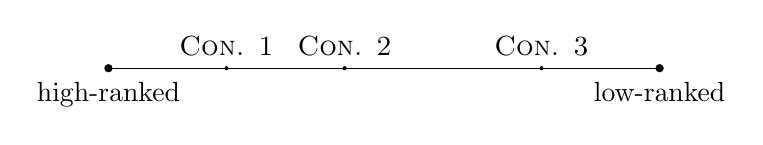
\begin{tikzpicture}
  \draw [circle, inner sep=0pt, minimum size=1.5pt] (0,0) -- +(7,0) ;
  \node[fill, label=below:{high-ranked}, circle, inner sep=0pt, minimum size=3.0pt] (d) at (0,0) {};  
  \node[fill, label=below:{low-ranked}, circle, inner sep=0pt, minimum size=3.0pt] (e) at (7,0) {};    
  \node[fill, label=above:\textsc{Con. 1}, circle, inner sep=0pt, minimum size=1.5pt] (a) at (1.5,0) {};
  \node[fill, label=above:\textsc{Con. 2}, circle, inner sep=0pt, minimum size=1.5pt] (b) at (3.0,0) {};  
  \node[fill, label=above:\textsc{Con. 3}, circle, inner sep=0pt, minimum size=1.5pt] (c) at (5.5,0) {};  
\end{tikzpicture}
\end{figure}

Now, the model has to implement a way to deal with gradient grammaticality, solving the many issues standard Optimality Theory has with modeling the implicit object construction (debated in \refsec{ot_bad_dobjdrop}). Stochastic Optimality Theory achieves this result by means of the Gradual Learning Algorithm, which is intended to be an improvement on the Constraint Demotion algorithm \parencite{TesarSmolensky1993learnability} used in standard Optimality Theory. Building a Stochastic Optimality Theoretic grammar is a sensible choice for linguists dealing with any phenomenon where a given input generates candidates with no unique winner, such as language change (with different winners at different times in history), language development (with different winners at different times in the child's life), and complex synchronic phenomena such as indefinite object drop (with different winners at the same time, based on the interaction of the semantic, aspectual, and pragmatic factors listed in \refch{factors}).\\
Stochastic Optimality Theory allows more than one candidate to be optimal at the same time by allowing constraints to "float" on the continuous scale, as if perturbed by numerical noise at the moment of evaluation. In practice, this is possible by assigning to each constraint a full range of values, centered on what was previously a single point on the scale (now called "ranking value"). Given the range of values, the specific value used at evaluation time is called an "evaluation point". Most importantly, the constraint ranking ranges are defined as probability distributions, and distribution overlap determines the probability of two constraints re-ranking with respect to one another. As illustrated in \reffig{stochot_gaussians1} and \reffig{stochot_gaussians2}, probability distributions in Stochastic Optimality Theory are \textit{normal} distributions. The Gaussian curves are defined by their mean value, which is the ranking value, and their standard deviation, which determines how broad the curve is.\sidenote{Let $\mu$ be the mean value of the distribution and $\sigma$ the standard deviation. The normal distribution is a function defined by the equation:
$$ f(x) = \frac{1}{\sigma\sqrt{2\pi}}e^{-\frac{1}{2}(\frac{x-\mu}{\sigma})^2} $$
} Since all constraints are assigned the same normal distribution in traditional Stochastic Optimality Theory, the actual value of the standard deviation (the "evaluation noise") has no effect on the constraint re-ranking, and it is arbitrarily set at 2 (a different approach to this matter is provided in \textcite{reynolds1994variation, nagy1997optimality}). At evaluation time, the selection point will occur most probably in correspondence of the ranking value (given the properties of normal distributions), and its probability steady declines as its value departs from the center of the distribution (i.e., the ranking value).\\
Going back to the simple state of affairs illustrated in \reffig{stot_contranking}, it is evident from \reffig{stochot_gaussians1} that the floating-constraint model makes it now possible for \textsc{Constraint 1} and \textsc{Constraint 2} to re-rank. In the picture, \textsc{Constraint 1} has a ranking value of 6.5 and \textsc{Constraint 2} a ranking value of 4, ordered from the higher-ranked to the lower-ranked as in the custom of Optimality Theory. In particular, as shown by the overlapping curves, the two constraints re-rank freely when the selection points are comprised between 4 and 6.5, and it is much more probable for \textsc{Constraint 1} to outrank \textsc{Constraint 2} than the opposite (graphically, there is only a small area where the curve for \textsc{Constraint 2} is above the curve for \textsc{Constraint 1}, for x values between 4 and 5.25).

\pgfmathdeclarefunction{gauss}{2}{%
  \pgfmathparse{1/(#2*sqrt(2*pi))*exp(-((x-#1)^2)/(2*#2^2))}%
}

\begin{figure}[htb]
\caption{Constraint re-ranking distribution in Stochastic Optimality Theory (overlapping constraints).}
\labfig{stochot_gaussians1}
\begin{tikzpicture}
\begin{axis}[
  no markers, domain=0:10, samples=100, xscale=-1,
  axis lines*=left, xlabel=$x$, ylabel=$y$, 
  every axis y label/.style={at=(current axis.above origin),anchor=south},
  every axis x label/.style={at=(current axis.left of origin),anchor=east},
  height=3cm, width=10cm, % height=5cm, width=12cm,
  xtick={4,6.5}, ytick=\empty,
  enlargelimits=false, clip=false, axis on top,
  grid = major
  ]
  \addplot [fill=cyan!20, draw=none, domain=0:6.5] {gauss(6.5,1)}
  \closedcycle;
  \addplot [fill=cyan!20, draw=none, domain=4:6.5] {gauss(4,1)}
  \closedcycle;
  \addplot [very thick,dotted,cyan!50!black] {gauss(4,1)};
  \addplot [very thick,cyan!50!black] {gauss(6.5,1)};
% \draw [yshift=-1.2cm, latex-latex](axis cs:4,0) -- node [fill=white] {$1.96\sigma$} (axis cs:5.96,0);
\draw [yshift=-0.5cm, latex-latex](axis cs:4,0) -- node [fill=white] {\textsc{Constr. 2}} (axis cs:4,0);
\draw [yshift=-0.5cm, latex-latex](axis cs:6.5,0) -- node [fill=white] {\textsc{Constr. 1}} (axis cs:6.5,0);
\end{axis}
\end{tikzpicture}
\end{figure}

Instead, \textsc{Constraint 2} and \textsc{Constraint 3} never re-rank with respect to one another, since their probability distributions in \reffig{stochot_gaussians2} never overlap (ranking values have been randomly assigned in the picture just for the argument's sake). In situations such as this, the constraint ranking on a continuous scale just reproduces the results of the categorical ranking yielded in standard Optimality Theory, i.e., strict domination.

\begin{figure}[htb]
\caption{Constraint re-ranking distribution in Stochastic Optimality Theory (non-overlapping constraints).}
\labfig{stochot_gaussians2}
\begin{tikzpicture}
\begin{axis}[
  no markers, domain=0:10, samples=100, xscale=-1,
  axis lines*=left, xlabel=$x$, ylabel=$y$,
  every axis y label/.style={at=(current axis.above origin),anchor=south},
  every axis x label/.style={at=(current axis.left of origin),anchor=east},
  height=3cm, width=10cm, % height=5cm, width=12cm,
  xtick={2,8}, ytick=\empty,
  enlargelimits=false, clip=false, axis on top,
  grid = major
  ]
%   \addplot [fill=cyan!20, draw=none, domain=0:5.96] {gauss(8,1)} \closedcycle;
  \addplot [very thick,dotted,cyan!50!black] {gauss(2,1)};
  \addplot [very thick,cyan!50!black] {gauss(8,1)};
% \draw [yshift=-1.2cm, latex-latex](axis cs:2,0) -- node [fill=white] {$1.96\sigma$} (axis cs:5.96,0);
\draw [yshift=-0.5cm, latex-latex](axis cs:2,0) -- node [fill=white] {\textsc{Constr. 3}} (axis cs:2,0);
\draw [yshift=-0.5cm, latex-latex](axis cs:8,0) -- node [fill=white] {\textsc{Constr. 2}} (axis cs:8,0);
\end{axis}
\end{tikzpicture}
\end{figure}

The Gradual Learning Algorithm uses these premises to assign an empirically motivated ranking value to each constraint, modulating its outcome based on an error-driven procedure. The full details of how the algorithm works, which the reader will find in \textcite{BoersmaHayes2001empirical}, are outside the scope of this chapter. For the purposes of my dissertation, it is important to note that Stochastic Optimality Theory provides an optimal environment to create a model of indefinite object drop. Let us consider a simple example such as \ref{mock_simple_dobj}, where the verb \textit{to eat} is used transitively in \ref{mock_simple_dobj1} and intransitively in \ref{mock_simple_dobj2}, and let us ignore the effect of the many factors influencing object drop (discussed in \refch{factors}) for the time being. Both \ref{mock_simple_dobj1} and \ref{mock_simple_dobj2} are grammatical, but the latter is judged slightly less acceptable than the former on average by some hypothetical native speakers of English.
% \vspace{-0.5cm} % PER AGGIUSTARE LO SPAZIO PRIMA DEGLI ESEMPI!
\ex. \label{mock_simple_dobj} \a. \label{mock_simple_dobj1} John is eating pizza. \hfill 7
\b. \label{mock_simple_dobj2} John is eating. \hfill 6.5

In our simplified model of object drop, we would posit just two conflicting constraints in the spirit of Optimality Theory (as explained in \refsec{classicot}): \textsc{*Internal Argument Structure}, a markedness constraint penalizing the presence of an overt direct object in the output, and \textsc{Faithfulness to Argument Structure}, a faithfulness constraint requiring all the arguments in the input to be also realized in the output. In a standard Optimality Theoretic analysis of the candidate set in \ref{mock_simple_dobj}, \textsc{Faithfulness to Argument Structure} would be ranked above \textsc{*Internal Argument Structure} and make \ref{mock_simple_dobj1} the only winner in the competition, with no reference to the slight acceptability difference. A Stochastic Optimality Theoretic model would solve the problem, so that \textsc{Faithfulness to Argument Structure} would indeed be ranked above \textsc{*Internal Argument Structure} most of the times, but with a large overlap between the two probability distributions (see \reffig{stochot_gaussians_dobj}). Crucially, one constraint outranks the other only probabilistically, while in the standard Optimality Theoretic model it would do so in an absolute sense due to strict domination.

\begin{figure}[htb]
\caption{Constraint re-ranking distribution in Stochastic Optimality Theory relative to Example \ref{mock_simple_dobj}.}
\labfig{stochot_gaussians_dobj}
\begin{tikzpicture}
\begin{axis}[
  no markers, domain=0:10, samples=100, xscale=-1,
  axis lines*=left, xlabel=$x$, ylabel=$y$, 
  every axis y label/.style={at=(current axis.above origin),anchor=south},
  every axis x label/.style={at=(current axis.left of origin),anchor=east},
  height=3cm, width=8cm, % height=5cm, width=12cm,
  xtick={5.5,6.5}, ytick=\empty, xticklabels={,,},
  enlargelimits=false, clip=false, axis on top,
  grid = major
  ]
%   \addplot [fill=cyan!20, draw=none, domain=0:6.5] {gauss(6.5,1)}
%   \closedcycle;
%   \addplot [fill=cyan!20, draw=none, domain=5.5:6.5] {gauss(5.5,1)}
%   \closedcycle;
  \addplot [very thick,dotted,cyan!50!black] {gauss(5.5,1)};
  \addplot [very thick,cyan!50!black] {gauss(6.5,1)};
% \draw [yshift=-1.2cm, latex-latex](axis cs:4,0) -- node [fill=white] {$1.96\sigma$} (axis cs:5.96,0);
\draw [yshift=2.0cm, latex-latex](axis cs:5.5,0) -- node [fill=white] {\textsc{*Int Arg}} (axis cs:5.5,0);
\draw [yshift=-0.5cm, latex-latex](axis cs:6.5,0) -- node [fill=white] {\textsc{Faith Arg}} (axis cs:6.5,0);
\end{axis}
\end{tikzpicture}
\end{figure}

The use of Stochastic Optimality Theory to define a working model of the implicit object construction, aware of the effect of the factors presented in \refch{factors} and of the fact that different transitive verbs are differently prone to be used intransitively, is the topic of \refch{medina}.
\setchapterstyle{kao}
\setchapterpreamble[u]{\margintoc}
\chapter{Linguistic factors used as predictors}
\labch{predictors}

This Chapter presents the five linguistic factors I will use as predictors in my Stochastic OT model of implicit indefinite objects, defined in \nrefch{modeltheory}. The theory linking each of these factors to the omissibility of direct objects is discussed at length in \nrefch{factors}.


\section{Recoverability} \labsec{predictor_sps}

% MEDINA PDF 32, aggiungere al mio paragrafo/capitolo su PISA!

%  In brief, these qualities include not stipulating verb meaning or selectional preferences but rather modeling a verb’s selection of argument classes in terms of production data, quantifying what a speaker knows about the meaning of a verb, and being able to compare the breadth of a verb’s selectional preferences across speakers and age periods.
% By distributing the credit for a particular noun over all of the argument classes which subsume it, the model is able to capture semantic generalizations. For example, the argument classes which subsume the noun “water” include water, liquid, fluid, substance, matter, physical entity, and entity (Fellbaum, 1998). Thus, what is computed by SPS is not only that a verb selected for the noun “water”, but rather that it selected for all the argument classes which subsume the noun, such as liquid. If only the particular nouns used were allowed in the model, then very few verbs would be highly selective since they would select for a wide range of non-identical objects. In contrast, by calculating SPS over argument classes, what can be generalized about a verb is that it tends to select nouns that fall under the classes of liquid, fluid, etc
% SPS can be computed over all senses of a noun, and thus over all of the argument classes which subsume each of these senses

As shown in \nrefsec{recoverability}, direct objects are likely omitted if they are "sufficiently recoverable" \parencite{Glass2013} from the meaning of the verb. Following \textcite{Medina2007}, object recoverability as a predictor in the Stochastic Optimality Theoretic model provided in this thesis is a continuous variable, for two main reasons. First, it would not be possible to set a fixed threshold value to separate recoverable and non-recoverable object verbs. Second, a continuous predictor works especially well within a model of \textit{gradient} grammaticality, such as the one hereby provided.\\
While Medina \hl{only} employs the taxonomy-based Selectional Preference Strength measure by \textcite{Resnik1993, Resnik1996}, I model object recoverability using \hl{three different measures of a verb's semantic selectivity as a proxy to object recoverability:}

\begin{itemize}
    \item SPS, the taxonomy-based Selectional Preference Strength measure by \textcite{Resnik1993, Resnik1996};
    \item Computational PISA, a novel distributional measure of Preference In Selection of Arguments by \textcite{CappelliLenciPISA};
    \item Behavioral PISA, a behavioral measure inspired by Computational PISA and computed as the Object Similarity measure by \textcite{Medina2007}.
\end{itemize}

These three measures are explained in full detail throughout this section.


\subsection{Resnik's SPS}\labsec{resnik_sps}
% Before turning to the details of PISA, a brief historical introduction is in order.
% \paragraph{Introduction}  

\paragraph{Description} \textcite{Resnik1993, Resnik1996} was the first to link the recoverability of direct objects to the selectional preferences of transitive verbs in a computational model, substantiating this claim by showing that his measure of selectional preference correlates well with plausibility and typicality judgments provided by human subjects. Resnik observed that the distribution of the classes of entities used as direct objects in a corpus regardless of the predicate (called "prior distribution") is different from the distribution of the same classes used as direct objects of a given verb (called "posterior distribution"), say, \textit{to grow}. A graphical representation of this observation is provided in \reffig{resnik_prior&posterior}.

\begin{center}
\begin{figure}[htb]
\caption{Hypothetical representation of the prior (on the left) and posterior (on the right) distribution of direct object classes with respect to the verb \textit{to grow}, adapted from \textcite[54]{Resnik1993}.}
\labfig{resnik_prior&posterior}
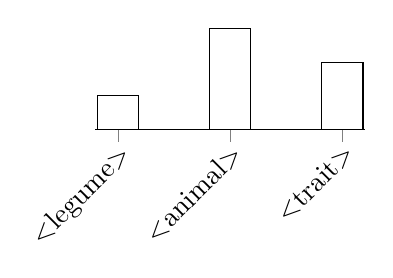
\begin{tikzpicture}
    \begin{axis}[
        ybar=1pt,
        bar width=15pt,
        ymin=0,
        width=5cm,
        height=3cm,
     hide y axis,
     axis x line*=bottom,
        symbolic x coords={$<$legume$>$, $<$animal$>$, $<$trait$>$},
        xtick = data,
        x tick label style={rotate=45, anchor=north east, inner sep=0mm},
        legend pos=north west
    ]
    \addplot[fill=none] coordinates {($<$legume$>$, 1) ($<$animal$>$, 3) ($<$trait$>$, 2)};
    \end{axis}
\end{tikzpicture}
\hspace{1cm}
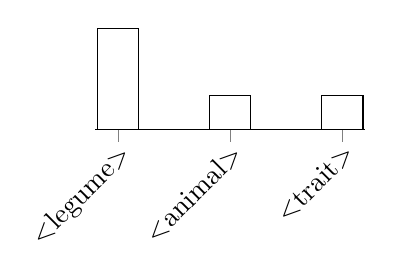
\begin{tikzpicture}
    \begin{axis}[
        ybar=1pt,
        bar width=15pt,
        ymin=0,
        width=5cm,
        height=3cm,
     hide y axis,
     axis x line*=bottom,
        symbolic x coords={$<$legume$>$, $<$animal$>$, $<$trait$>$},
        xtick = data,
        x tick label style={rotate=45, anchor=north east, inner sep=0mm},
        legend pos=north west
    ]
    \addplot[fill=none] coordinates {($<$legume$>$, 3) ($<$animal$>$, 1) ($<$trait$>$, 1)};
    \end{axis}
\end{tikzpicture}
\end{figure}
\end{center}

Under this view, selectional preferences are fully encoded by the change between the prior and the posterior distribution. Resnik implemented this intuition with his Selectional Preference Strength (SPS) measure, defined as the Kullback-Leibler divergence (relative entropy) between the two distributions, as in \refeq{resnik_sps_eq}.

\begin{equation} \labeq{resnik_sps_eq}
SPS_{v,r} = \sum_{c \in classes} p(c|v,r) \: \log_{2}\frac{p(c|v,r)}{p(c|r)}
\end{equation}

In \refeq{resnik_sps_eq}, $p(c|v,r)$ is the posterior distribution of argument classes for a given predicate $v$ in a given relation $r$ with the predicate, and $p(c|r)$ is the prior distribution of argument classes regardless of the predicate. The only relevant relation for the purposes of this thesis is the verb-object relation, but it can also be any other grammatical function (such as verb-subject) or semantic role (such as verb-Instrument, as in \textcite{CappelliLenciPISA}). Given a set of transitive verbs used in a corpus, SPS scores will be higher for transitive verbs having a narrow selectional range (as in \ref{dobj1}) and lower for those having a broader selectional range (as in \ref{dobj2}).
\ex.\label{ex1} \a. \label{dobj1} John ate $\varnothing$\textsubscript{object}.
\b. \label{dobj2} *John made $\varnothing$\textsubscript{object}.

Crucially, selectional preferences as measured by SPS provide insight about the recoverability of direct objects, and their recoverability affects the grammaticality of the sentences in \ref{ex1}. In particular, \textit{to eat} selects mostly for edible items, so that reading \ref{dobj1} we can reasonably assume John ate some kind of food, while \textit{to make} selects for a wide array of objects from semantically different classes, so it's impossible to know what is that John made in \ref{dobj2}.\\
The classes considered when computing the SPS scores have to belong to a lexical taxonomy, so that each sense of each noun in the lexicon is mapped to a concept. Using Resnik's example \parencite[59]{Resnik1993}, the noun \textit{baseball} can be mapped to two concepts, i.e. a hyponym of the concept $<$ball$>$ and a hyponym of the concept $<$field game$>$. Moving from concepts to taxonomy classes, a noun belongs to any class having one of its concepts as a hyponym, even indirectly. Thus, as illustrated in \reffig{wordnet_simplified}, \textit{baseball} belongs not only to the classes $<$ball$>$ and $<$field game$>$, but also to $<$game equipment$>$, $<$artifact$>$, $<$inanimate object$>$, $<$outdoor game$>$, $<$sport$>$, $<$human activity$>$, and $<$entity$>$ (the root node of the whole hierarchy).

\begin{figure}[htb]
\caption{Simplified representation of the noun \textit{baseball} in the lexical taxonomy.}
\labfig{wordnet_simplified}
\centering
\begin{forest}
[$<$entity$>$
  [$<$inanimate object$>$
    [$<$artifact$>$
      [$<$game equipment$>$
        [$<$ball$>$,name=S1 [\textit{baseball},phantom]
        [...,tier=mytier]
        [...,tier=mytier]
        [...,tier=mytier]
        ] 
  [...
  ]
      ]
  [...
  ]
    ]
  [...
  ]
  ]
  [\textit{baseball},tier=mytier,no edge,name=shared]
  [...
  ]
  [$<$human activity$>$
    [$<$sport$>$
        [$<$outdoor game$>$
            [$<$field game$>$,name=S2 [\textit{baseball},phantom]
        [...,tier=mytier]
        [...,tier=mytier]
        [...,tier=mytier]
            ]
  [...
  ]
        ]
  [...
  ]
    ]
  [...
  ]
  ]
]
\draw (S2) -- (shared);
\draw (S1) -- (shared);
\end{forest}
\end{figure}

In order to compute SPS scores, Resnik adopts WordNet \parencite{beckwith1991wordnet,Miller1995} as a computational model of the lexical taxonomy. Its appeal to the author \parencite[32]{Resnik1993} lies in that the WordNet taxonomy encodes knowledge in an explicit, hierarchical fashion, which is "intuitively reasonable" and "widely accepted".\\ While powerful in many respects, Resnik's model of selectional preferences has a crucial drawback, which is the need for a manually-built lexicon. This requirement makes it difficult to compute SPS scores for verbs in languages without a WordNet, for neologisms, and for special registers not yet encoded in WordNet. Given this severe limitation, I decided \hl{to improve on} Resnik's SPS to model the recoverability of direct objects, creating a model based on distributional semantics \parencite{Lenci:2018} that can be applied in all the cases where the SPS measure cannot.

\paragraph{Results}
The SPS scores for the English and Italian transitive verbs under consideration are fully listed in \refappsec{app_resnik}.\\ % \vspace{}

\subsection{Computational PISA}\labsec{compuPisa}

Distributional semantics is based on the Distributional Hypothesis, which states that words occurring in the same contexts tend to have similar meanings, or, quoting the popular formula from \textcite{firth1957synopsis}, that "you shall know a word by the company it keeps". Such a framework puts the meaning of words in the ever-changing use speakers make of language, instead of securing it in the nodes of a static lexical taxonomy. Most importantly, distributional semantics posits a correlation between distributional similarity and semantic similarity and uses the former to model the latter. Roughly, the semantic space where words "keep company" can be modeled as a vector space where each word is a vector whose dimensions are context words. An example is provided in \reffig{vectorspace}, where the two words \textit{hamburger} and \textit{dragon} populate a semantic space defined by the three context words \textit{big}, \textit{tasty}, and \textit{mythological}. The coordinates of \textit{hamburger} are (2,2,0) because in this hypothetical situation it occurs twice with \textit{big}, twice with \textit{tasty}, and never with \textit{mythological}, while the coordinates of \textit{dragon} are (2,0,1) because it occurs twice with \textit{big}, never with \textit{tasty}, and once with \textit{mythological} in the hypothetical corpus.

\begin{figure}[htb]
\caption{Simplified representation of the words \textit{hamburger} and \textit{dragon} in a vector space.}
\labfig{vectorspace}
\centering
\begin{tikzpicture}[x=1cm, y=1cm, z=-0.6cm]
    % Axes
    \draw [->] (0,0,0) -- (4,0,0) node [right] {$big$};
    \draw [->] (0,0,0) -- (0,4,0) node [left] {$tasty$};
    \draw [->] (0,0,0) -- (0,0,4) node [left] {$mythological$};
    % Vectors
    \draw [->, thick] (0,0,0) -- (2,2,0);
    \draw [->, thick] (0,0,0) -- (2,0,1);
    % Ticks
        \foreach \i in {1,2}
    {
    \draw (-0.1,\i,0) -- ++ (0.2,0,0);
    \draw (\i,-0.1,0) -- ++ (0,0.2,0);
    \draw (-0.1,0,\i) -- ++ (0.2,0,0);
    }
    % Dashed lines
    \draw [loosely dashed]
        (0,2,0) -- (2,2,0) -- (2,0,0)
        (0,0,1) -- (2,0,1) -- (2,0,0)
        ;
    % Labels
     \node [right] at (2,2,0) {hamburger};
   \node [below] at (2,0,1) {dragon};

\end{tikzpicture}
\end{figure}

How does all of this translate into a solution to the problem of having a taxonomy-free model of argument recoverability? Let us go back to the example in \ref{ex1} and consider the distribution of the arguments of the two verbs \textit{to eat} and \textit{to make} in a corpus. Ideally, collapsing on a 2-dimensional grid the $n$-dimensional space populated by these arguments, the distribution of the arguments of \textit{to eat} would resemble \reffig{mock_args_eat} and the distribution of the arguments of \textit{to make} would resemble \reffig{mock_args_make}. The (recoverable) arguments of \textit{to eat} are close together in the vector space, while the (non-recoverable) arguments of \textit{to make} are very sparse in the same space.

\begin{figure}[htb]
\caption{Made-up representation of the possible distribution of the direct objects of the verb \textit{to eat} in a vector space.}
\labfig{mock_args_eat}
\centering
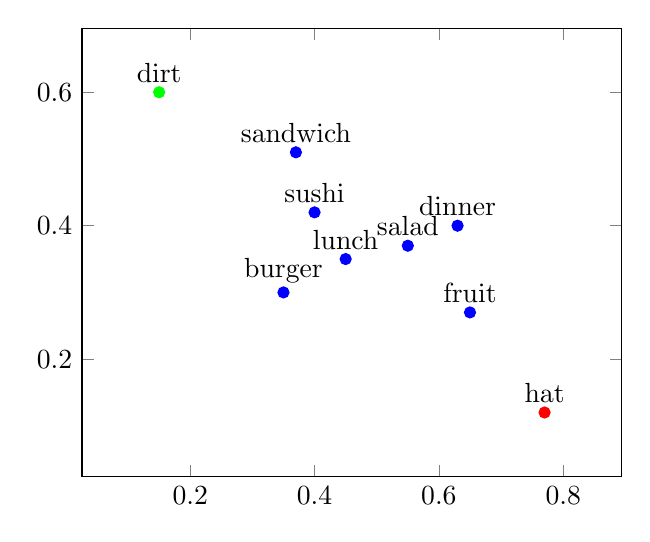
\begin{tikzpicture}
\begin{axis}[enlargelimits=0.2]
    \addplot[
        scatter/classes={a={blue}, b={red}, c={green}},
        scatter, mark=*, only marks, 
        scatter src=explicit symbolic,
        nodes near coords*={\Label},
        visualization depends on={value \thisrow{label} \as \Label} %<- added value
    ] table [meta=class] {
        x y class label
        0.63 0.4 a dinner
        0.45 0.35 a lunch
        0.4 0.42 a sushi
        0.55 0.37 a salad
        0.37 0.51 a sandwich
        0.35 0.3 a burger
        0.65 0.27 a fruit
        0.77 0.12 b hat
        0.15 0.6 c dirt
    };
\end{axis}
\end{tikzpicture}
\end{figure}

\begin{figure}[htb]
\caption{Made-up representation of the possible distribution of the direct objects of the verb \textit{to make} in a vector space.}
\labfig{mock_args_make}
\centering
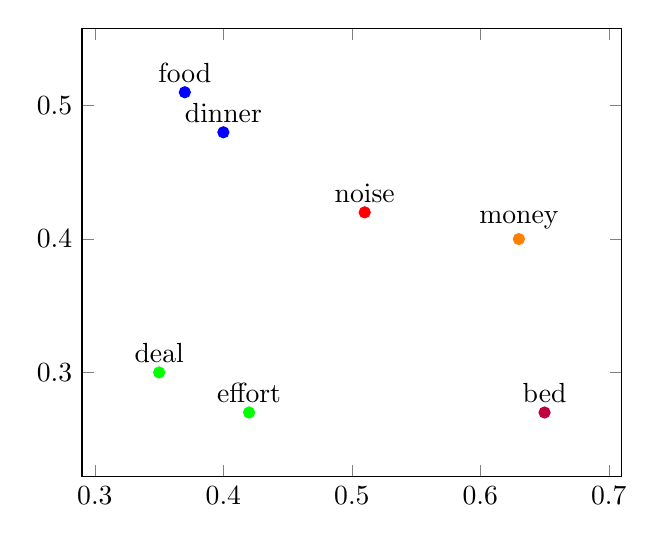
\begin{tikzpicture}
\begin{axis}[enlargelimits=0.2]
    \addplot[
        scatter/classes={a={blue}, b={red}, c={green}, d={orange}, e={purple}},
        scatter, mark=*, only marks, 
        scatter src=explicit symbolic,
        nodes near coords*={\Label},
        visualization depends on={value \thisrow{label} \as \Label} %<- added value
    ] table [meta=class] {
        x y class label
        0.37 0.51 a food
        0.4 0.48 a dinner
        0.63 0.4 d money
        0.51 0.42 b noise
        0.42 0.27 c effort
        0.35 0.3 c deal
        0.65 0.27 e bed
    };
\end{axis}
\end{tikzpicture}
\end{figure}

Based on these consideration, the conclusion is that the closer the direct objects of a verb are in a vector space, the more recoverable they should be. This is the main intuition behind Computational PISA, whose computational implementation I will discuss in the next paragraph.

\paragraph{Computational implementation} Computational PISA is defined as the semantic density of a verb-relation pair, i.e. the mean value of the pairwise cosine similarity between the arguments of the pair. In this thesis, this means calculating the mean pairwise cosine similarity between all the direct objects of a given transitive verb. \hl{The full script used to obtain Computational PISA scores using a corpus and a list of verbs as input is available} \href{https://github.com/ellepannitto/PISA}{on GitHub}\sidenote{https://github.com/ellepannitto/ PISA}. \\
This is done in two steps, for each transitive verb under consideration. The first one is to compute the Selectional Association between the verb and each one of its direct objects as defined by \textcite{Erk2007, ErkEtAl2010} in \refeq{erkpadopado}. This is a measure of the strength of the selectional preference \textit{SA} of a verb for a possible argument \textit{a\textsubscript{0}}, modeled as the weighted sum of the similarities between the candidate argument \textit{a\textsubscript{0}} and the actual arguments found in the corpus (each called \textit{a} in the formula). In \textcite{CappelliLenciPISA} and this dissertation I measure argument similarity with the cosine similarity.

\begin{equation} \labeq{erkpadopado}
SA_{v,r} (a_0) = \sum_{a \in args(v,r)} wt_{v,r}(a) \: sim(a_0,a)
\end{equation}

Then, Computational PISA scores are computed as in \refeq{pisa}, i.e. by averaging \refeq{erkpadopado} over the \textit{n} direct objects of a given transitive verb.

\begin{equation} \labeq{pisa}
PISA_{v,r} = \frac{1}{n} \sum_{i = 1}^{n} SA_{v,r} (a_i)
\end{equation}

In \textcite{CappelliLenciPISA} five weight functions are used to compute \refeq{erkpadopado} and then \refeq{pisa} (\refeq{uni}, \refeq{freq}, and \refeq{idf} are taken from \textcite{ErkEtAl2010}). In detail, the functions are as follows.
\begin{itemize}

\item \textbf{UNI} assumes a uniform distribution. This actually yields an \textit{un}weighted model, because in \refeq{erkpadopado} the argument similarity is always multiplied by 1.
\begin{equation} \labeq{uni}
wt_{v,r}(a) = 1
\end{equation}

\item \textbf{FRQ} is the co-occurrence frequency of a given direct object with the transitive verb under consideration.
\begin{equation} \labeq{freq}
wt_{v,r}(a) = freq(a,v,r)
\end{equation}

\item \textbf{IDF} is inspired to the well-known Inverse Document Frequency weighting scheme, which
assigns higher scores to direct objects occurring with fewer transitive verbs (the minimum would be 0, for an argument that occurs with every verb in the corpus). This is done in order to mitigate the frequency effect of arguments occurring with too many verbs to be considered relevant for the specific target verb under examination. In \refeq{idf}, $|v,r|$ is the number of transitive verbs in the corpus, and $|v,r : a \in v,r|$ is the number of transitive verbs having $a$ as a direct object.
 \begin{equation} \labeq{idf}
wt_{v,r}(a) = \log _{} \frac{|v,r|}{|v,r : a \in v,r|}
\end{equation}

\item \textbf{LMI} is the Local Mutual Information \parencite[89]{evert2005statistics-lmi} of the direct object and a given transitive verb, computed as in \refeq{lmi}. The LMI compares the probability of a noun occurring in a corpus as the direct object of a verb with the probability of the noun and the transitive verb occurring in a corpus without any relation to one another. In other words, given a noun and a transitive verb, their LMI is computed as the logarithmic ratio of their joint probability and the product of their individual probabilities in the corpus (i.e. their joint probability if they were statistically independent events).
 \begin{equation} \labeq{lmi}
wt_{v,r}(a) = f(a,v,r) \log _{2} \frac{p(a,v,r)}{p(a)p(v,r)}
\end{equation}  

\item \textbf{ENT} is the entropy \parencite{shannon1948mathematical} of the direct objects of a given transitive verb. Information theory uses entropy to quantify the informativity of a given event, inheriting its mathematical definition from thermodynamics. The entropy of an event (which in \refeq{ent} is the argument itself) is a function whose value decreases as the probability of the event increases.
 \begin{equation} \labeq{ent}
wt_{v,r}(a) = -\!\sum_{\mathclap{a \in args(v,r)}} p(a) \log _{2}p(a)
\end{equation}
In \refeq{ent}, $p(a) = \frac{f(a)}{\sum_{a_0 \in A}f(a_0)}$, where $A$ is the complete set of the direct objects of the target verbs, extracted from the corpus.
\end{itemize}

\paragraph{The original experiment}
In \textcite{CappelliLenciPISA}, I computed weighted models of argument recoverability, as explained in the previous paragraph, and also unweighted models, only taking into account 300 direct objects for each transitive verb. For each verb, the relevant 300 objects were selected after sorting the entire list of direct objects based on the FRQ, IDF, LMI and ENT functions. The reason to include unweighted models in the experiment stems from the observation that the computation of \refeq{pisa} for verbs with a large number of direct objects can get cumbersome, and it may be possible to achieve a comparable degree of informativity by only considering the most relevant objects occurring with each verb.\\
I tested the models on a 99-verb set of transitive verbs, extracting their direct objects from ukWaC, a 2-billion token part-of-speech tagged and lemmatized corpus of English \parencite{FerraresiEtAl2008}. Direct objects were modeled as bare head nouns, excluding any determiner and modifier present in the DP (e.g. \textit{sword} instead of \textit{a big rusty sword}). I obtained the vector representation of direct objects by using 12 different 300-dimensional embeddings trained on a concatenation of ukWaC and a 2018-dump of English Wikipedia, including both SVD-reduced count-based DSMs and neural embeddings.\\
Since Computational PISA was intended to model argument recoverability, I tested the results of each model by means of a Mann-Whitney U test comparing the mean Computational PISA score of the recoverable-object transitive verbs with the mean Computational PISA score of the non-recoverable-object transitive verbs. Summing up the discussion of the results carried out in the original paper (here in \reftab{tab:mwu}), it was found that the weighted versions of Computational PISA yield highly significant results, while the unweighted versions yield results with a comparable degree of significance just with the FRQ sorting function and, in particular, running the model on word2vec \parencite{mikolov2013efficient} distributional spaces.

\begin{table}
\caption{Mann-Whitney U tests comparing recoverable- and non-recoverable-argument verbs (significance levels).}
\labtab{tab:mwu}
\centering
\begin{small}
\begin{tabular}{llccc}
\hline & & \textbf{weighted} & \textbf{top $k$} & \textbf{bot $k$} \\ \hline
 & SVD & *** & - & - \\
\texttt{\textbf{UNI}} & w2v & *** & - & - \\
 & w2vf & ** & - & - \\
 \hline
 & SVD & *** & ** & ns \\
\texttt{\textbf{FRQ}} & w2v & *** & *** & ns \\
 & w2vf & *** & ** & ns \\
 \hline
 & SVD & *** & ** & ns \\
\texttt{\textbf{IDF}} & w2v & *** & *** & *** \\
 & w2vf & ** & ns & ns \\
 \hline
 & SVD & *** & ** & ns \\
\texttt{\textbf{LMI}} & w2v & *** & * & * \\
 & w2vf & *** & * & * \\
 \hline
 & SVD & *** & ns & ns \\
\texttt{\textbf{ENT}} & w2v & *** & *** & ns \\
 & w2vf & *** & * & * \\
\hline
\end{tabular}
\end{small}
\end{table}

\paragraph{\hl{Operative choices}}
Drawing from the results discussed in \textcite{CappelliLenciPISA} and summarized in the previous paragraph, I computed Computational PISA scores for my verbs of interest in English and Italian. For English, I based the calculations on ukWaC as in the original study, and for Italian, I based them on itWaC, a 2-billion token part-of-speech tagged and lemmatized corpus of Italian \parencite{baroni2009wacky}. Given that web-scraped, automatically tagged corpora this large inevitably suffer from significant noise in the data, which then results in possibly unreliable results, I pre-processed the data extracted from both corpora to minimize the impact of noise and tagging mishaps. First of all, I filtered the 65,000 direct objects of my 30+30 verbs of interest so that they were:
\begin{itemize}
    \item not hapaxes (considering the verb-noun frequencies)
    \item having an absolute frequency in the corpus greater than 100
    \item present in WordNet (to eliminate misspelled words)
\end{itemize}
Then, I manually filtered the remaining nouns so that each verb only takes direct objects which do not belong to any of these categories:
\begin{itemize}
    \item idiomatic senses (e.g. 'ice' as an object of 'to break')
    \item metaphoric senses (e.g. 'mind' as an object of 'to poison')
    \item direct objects of an unintended meaning of the verb (e.g. 'salmon' as an object of 'to smoke', since the intended sense of 'to smoke' in my study is only the one related to inhaling the byproduct of the combustion of tobacco and other plants)
    \item unintended direct objects (e.g. Recipients in double-object constructions such as 'pupils' in 'to teach pupils Linguistics', since in my study I am only interested in Theme/Patient direct objects)
    \item mistagged direct objects (e.g. 'disorder' as an object of 'to eat', which is clearly the result of the automatic corpus tagger interpreting 'eating' in 'eating disorder' as a verb rather than as an adjective)
    \item 'thing' (and 'stuff'), which appears with every transitive verb and is thus irrelevant
\end{itemize}
The files containing the complete list of direct objects of each verb, both raw and cleaned, both in English and in Italian, are freely available \href{https://github.com/giuliacappelli/dissertationData}{on my GitHub profile}\sidenote{https://github.com/giuliacappelli/ dissertationData}.\\
I based my operative choices regarding the vector spaces and weighting functions on the results I obtained in the original Computational PISA study. In particular, I computed word2vec neural embeddings with the Python library Gensim with the same parameters for English and Italian, i.e. Skipgram with Negative Sampling (SGNS) with 5 noise words, window of 10 words, 300-dimension vectors, ignoring all words with an absolute frequency lower than 10. Among the five functions defined in \textcite{CappelliLenciPISA}, I employed the FRQ weighting function because it is the best-performing among all five, both in weighted and in sorted models of Computational PISA.

\paragraph{Results}
The Computational PISA scores for the English and Italian transitive verbs under consideration are fully listed in \refappsec{app_cpisa}.\\ % \vspace{}


\subsection{\hl{Behavioral PISA}}\labsec{behavPisa}

\paragraph{Introduction} 
Despite representing a clear step forward compared to Resnik's taxonomy-based measure of selectional preferences, a corpus-based measure such as Computational PISA still has notable downsides. First of all, the corpus on which Computational PISA calculations are based has to be large enough to feature all the verbs under consideration, and for each verb to present a sufficient number of direct objects to allow for the computation of meaningful Computational PISA. It may well be the case that using a small corpus forces an experimenter to draw from a different set of verbs than intended for their study, if not all of them are featured in the corpus. Moreover, low-frequency verbs may appear with a small set of direct objects even in large corpora, making it potentially difficult to obtain reliable Computational PISA scores. Another order of problems (which larger, automatically-tagged corpora are more prone to suffer from than smaller, manually-tagged ones) depends on noisy or otherwise inaccurate corpus data. For instance, large corpora constructed via crawling the Web (such as ukWaC and itWaC) typically present a substantial number of misspelled words and mis-tagged parts of speech, making it necessary to clean them manually beforehand. In addition to this, even clean corpora often lack fine-grained semantic information, about thematic roles (e.g. distinguishing the Theme and the Recipient in 'John gave Mary a book'), polysemy (e.g. 'to graduate' may mean 'to become a doctor', but also 'to arrange something in gradations'), idiomatic uses of verbs (e.g. there is usually no actual bucket being kicked when someone 'kicks the bucket').\\
In order to overcome these problems and obtain equally reliable scores for each verb in my experiment, I decided to implement a behavioral variant of the original Computational PISA measure. In the case of Behavioral PISA, the semantic similarity of a given verb's direct objects is not approximated via their distributional similarity in a corpus, but instead via their psychological similarity as judged by native speakers of the languages under study. Such a measure is intended to provide robust data for each verb regardless of its corpus frequency or scarcity of direct objects with respect to other verbs, at the cost of having to perform a behavioral experiment with human subjects.

\paragraph{Experimental protocol}
The experimental procedure to obtain the relevant data and compute the Behavioral PISA scores follows closely the method Medina used in her thesis to compute a comparable measure, which she calls "Object Similarity" \parencite[173-178]{Medina2007}, and whose purpose is to overcome the shortcomings of Resnik's SPS. In a sense, Object Similarity may be viewed as a behavioral precursor of Computational PISA, both being based on a broad notion of selectivity-as-semantic-closeness.\\
In order to build the stimuli, I picked 6 pairs of direct objects for each verb of interest in my two 30-verb sets (one for English and one for Italian, as detailed in \nrefch{judgments}). For each verb, the direct objects comprising the 6 pairs were randomly selected from the manually cleaned (see \nrefsec{compuPisa}) verb-object lists, so that each pair contained two different direct objects. This operation resulted in 180 stimuli (30 verbs x 6 direct objects) for each language, which the interested reader will find in \refapp{app_behavPisa}. Each pair of direct objects works as a stimulus, without explicit mention of the verb which subcategorizes the objects in the pair.\\
The two lists of 180 stimuli was used to create two Google Form surveys (with randomized stimuli), and 25 unpaid raters were recruited online for each language among native speakers holding at least a Bachelor's degree. Each rater had to judge the similarity of the two objects in each pair on a 7-point Likert scale in a single experimental session. Crucially, the participants to the experiment were not provided with a strict definition of similarity, and they did not know that the stimuli were direct objects of a given set of verbs. Instead, they were told that the pair 'love - upholstery' should get a rating of 1 an the pair 'cat - dog' should get a rating of 7, to familiarize them with the Likert scale, and they were encouraged to make use of the whole 7-point scale whenever necessary.

\paragraph{Computational implementation} Behavioral PISA is defined as the mean pairwise similarity between a subset of direct objects of a transitive verb. The pairwise similarity is obtained via human similarity judgments on a 7-point Likert scale, as described right above. In order to account for individual differences in the use of the scale, I computed the within-subject z-scores of these results, and then I averaged the normalized scores to obtain a single value for each verb of interest \parencite{KimEtAl2018, KimEtAl2019, KimEtAl2019a} as in \refeq{eq_behavPisa}, where $r$ is a (normalized) rating and $i$ is the total number of ratings.

\begin{equation} \labeq{eq_behavPisa}
PISA_{v} = \frac{\sum_{i} r_{v}}{i}
\end{equation}

The Behavioral PISA scores thus obtained were then normalized to fall between 0 and 1. The Python script I coded to generate the stimuli and compute the Behavioral PISA scores for each verb is freely available \href{https://github.com/giuliacappelli/behavioralPISA}{on my GitHub profile}\sidenote{https://github.com/giuliacappelli/ behavioralPISA}.

\paragraph{Results} 
The Behavioral PISA scores for the English and Italian transitive verbs under consideration are fully listed in \refappsec{app_bpisa}.\\ 

\section{Telicity} \labsec{predictor_telicity}

% Most importantly, under the definition of telicity as a privative opposition by \textcite[33]{Olsen1997telicity-privative} (implemented in the Stochastic Optimality Theoretic model of object omissibility by \textcite{Medina2007}), "no constituent may cancel the marked interpretation: [+telic] verbs are always interpreted as having an inherent end", while "atelicity is a cancelable conversational implicature".\\

\subsection{Telicity tests}
\nrefsec{telicity} introduced telicity as a major predictor of object omissibility. Since aspectual interpretation is compositional \parencite[14]{Olsen1997}, a transitive verb which can be used both transitively and intransitively tends to get a telic interpretation in the first case and an atelic interpretation in the second case.\\ 
In my behavioral experiments and subsequent linguistic models of object drop, I operationalize telicity as a binary feature, based on theoretical claims discussed before. A verb is considered [+Telic] if two tests yield a telic interpretation, [-Telic] otherwise. Out of Medina's set, I only used the staple \textit{in/for} test for telicity, rejecting the \textit{almost} test since it is notoriously quite problematic with achievements (please refer to \textcite{bertinetto-delfitto2000aspect} for an extensive discussion on the issue).\\
Verbs were tested without a direct object to avoid involuntarily eliciting a telic interpretation, or with a generic object (e.g. "something") if the intransitive use yields a grammatically unacceptable interpretation. The two tests used for the experiments of this thesis are as follows (the reader is referred to \textcite{Borik2006} and \textcite{Liu2014} for a detailed review of telicity tests)\sidenote{I also considered the \textit{conjunction} test for telicity, but then decided to discard it because it is weaker than the other two. This diagnostic requires that the predicate be tested in a sentence where it it modified by two conjoined temporal adjuncts denoting consecutive time slots, as in \ref{conj_test}. Telic verbs in this construction, as in \ref{conj_telic}, imply two separate events (i.e. John built something on Saturday and something else on Sunday). On the contrary, sentences with atelic verbs, as \ref{conj_atelic}, can be interpreted either as two separate events (i.e. John sang on Saturday, stopped, and resumed his singing on Sunday) or as a continuous event (John sang on both days without interruption).
\ex.\label{conj_test} \a. John built something on Saturday and on Sunday. \label{conj_telic} 
\b. John sang on Saturday and on Sunday. \label{conj_atelic}}.

\paragraph{\textit{In/for} test} Based on this largely agreed-upon diagnostic for telicity, telic predicates (e.g. \textit{build} in \ref{infor_telic}) are only grammatical if used with time-frame adverbials such as "in X time", while atelic predicates (e.g. \textit{sing} in \ref{infor_atelic}) are grammatical if used with time-span adverbials such as "for X time".
\ex. \label{infor_telic} \a. John built something in an hour.
\b. \%John built something for an hour.

\ex. \label{infor_atelic} \a. *John sang in an hour.
\b. John sang for an hour.

\paragraph{\textit{Progressive} entailment test} The progressive form of a predicate bears different pragmatic implicatures based on whether it is telic or atelic. In particular, saying that the subject "was \textit{verb}ing" implies that they \textit{verb}ed with atelic verbs as in \ref{progressive_atelic}, while this is not true for telic verbs as in \ref{progressive_telic}.
\ex. \a. John was building something. \label{progressive_telic} 
\b. John was singing. \label{progressive_atelic}

\subsection{Results}
The telicity features of each English and Italian transitive verb are listed in \refappsec{app_telicity}.



\section{Perfectivity} \labsec{predictor_perfectivity}

Perfectivity is discussed at large as a possible determinant of object drop in \nrefsec{perfectivity}. The main point is that transitive verbs resist the omission of their direct object when used in the perfective aspect (as in \ref{perf_ex1}), while verbs in the imperfective aspect are much more likely to allow it (as in \ref{perf_ex2}).
\ex.\label{perf_ex} \a. ? John painted. \label{perf_ex1} 
\b. John was painting. \label{perf_ex2}

Like telicity, perfectivity appears as a binary feature in my experiments and models. Unlike telicity, perfectivity is not an inherent feature of verbs, so it cannot be tested beforehand: instead, I will include it in the behavioral experiments by having both perfective and imperfective uses of the same verb (please refer to \nrefch{judgments} for a complete overview of the experimental design). The reader will find the results of these operative choices in \refapp{app_stimuli}.

\subsection{A note on tense}
To choose the correct tenses to encode (im)perfectivity in English and in Italian, a critical discussion on the relation between tense and aspect is in order. A common perspective on grammatical aspect in English, as summarized by \textcite[106]{smith1991parameter} and \textcite[663]{wagner2001aspectual}, is that perfective aspect corresponds to the simple form of the verb, while the imperfective aspect is derived by means of the progressive construction (i.e. by adding the auxiliary \textit{be} and \textit{-ing} to the main verb). This perspective has the undeniable merit of keeping grammatical aspect and lexical aspect apart, acknowledging the orthogonality of (a)telicity and (im)perfectivity (refer to \textcite{bertinetto2001frequent} for an extensive discussion on the issue). However, the view that the simple form of a verb is necessarily interpreted as perfective has long since been abandoned.\\
Based on \textcite{Olsen1997, bertinetto2001frequent}, the simple past in English is not marked for the perspective aspect. On the contrary, simple verb forms are aspectually unmarked, and they get different aspectual interpretations based on the interaction of tense, lexical aspect, and the different context they appear in. For this reason, for the experimental stimuli I will choose tenses that are aspectually marked, as to avoid misinterpretations.\\
Even though simple past does not equate to perfective aspect, it's true that past tense hints towards perfectivity, as noted by \textcite{comrie1976aspect} and later on by \textcite{wagner2001aspectual, Olsen1997, Medina2007}, among others. So, a morphologically unmarked past form is more likely to be interpreted as perfective than a non-past form. Moreover, there are differences internal to the group of past forms. In fact, as we saw before, the simple past is aspectually unmarked, but the past perfect (e.g. \textit{John had written a book.)} is marked as perfective.

\subsection{Operative choices}
Considering what has been noted in the previous paragraph, and following \textcite{Medina2007}, in the experimental stimuli perfective aspect will be encoded with perfect morphology and imperfective aspect will be encoded with progressive morphology.\\
For English, perfective stimuli will be in the past perfect tense (as in \ref{perf_ex1_eng}) and imperfective stimuli in the past continuous tense (as in \ref{perf_ex2_eng}). For Italian, perfective stimuli will be in the \textit{\hl{tra}passato prossimo} tense (as in \ref{perf_ex1_ita}) and imperfective stimuli in the continuous past form created with the auxiliary 'to stay' in the \textit{imperfetto} tense and the simple gerund of the main verb (as in \ref{perf_ex2_ita}). 
\ex.\label{perf_ex_eng} \a. John had played. \label{perf_ex1_eng} 
\b. John was playing. \label{perf_ex2_eng}

\ex.\label{perf_ex_ita} \a. Gianni \hl{aveva} cantato. \label{perf_ex1_ita} 
\b. Gianni stava cantando. \label{perf_ex2_ita}

On a side note, Italian also has perfective-only and imperfective-only simple past tenses, namely \textit{passato remoto} and \textit{imperfetto}, but I chose to use compound tenses since \textit{passato remoto} lost some ground to \textit{passato prossimo} over the last few decades, and also considering the variety of regional uses of \textit{passato remoto} \parencite{bertinetto1996distribuzione}. \hl{Most importantly, the \textit{trapassato} \textit{prossimo} tense was chosen to encode perfective aspect in Italian because it's the aspectually closest Italian tense to the English past perfect, despite the glaring differences between the aspectual systems in these two languages (Bertinetto 1992)}.

% QUI DEVO CITARE \parencite{bertinetto1992piucheperf}, CHE PER QUALCHE MOTIVO CREA ERRORI ANCHE SE FORMALMENTE SEMBRA CORRETTO

% Il mio suggerimento di rifare l'esperimento nasce dal fatto che occorre sempre confrontare (nei limiti del possibile) gli stessi oggetti. Questo principio viene violato se si confrontano piucheperfetto da un lato, e passato 'prossimo' dall'altro.

\section{Iterativity} \labsec{predictor_iterativity}

As argued in \nrefsec{iterativity}, iterativity and other types of pluractionality favor the omission of direct objects (compare \ref{iterat_ex1} and \ref{iterat_ex2}). Although well-known in the theoretical literature \parencite{Glass2013, Glass2020, Ruda2017}, to my knowledge this predictor of object drop appears here for the first time in a comprehensive linguistic model based on acceptability judgments.
\ex.\label{iterat_ex} \a. \# The Joker killed. \label{iterat_ex1} 
\b. The Joker killed again. \label{iterat_ex2}

Iterativity is yet another binary predictor and it will be encoded in the behavioral experiments in the same way as perfectivity, that is to say, by creating both iterative and non-iterative stimuli for the same verb as in \ref{iterat_ex} (please refer to \refapp{app_stimuli} for the complete set).

\section{Manner specification} \labsec{predictor_mannspec}

The effects of manner specification on indefinite object drop are presented in \nrefsec{mannerspec}. As argued by \textcite{Ruda2017} a.o., if a transitive verb allows for its direct object to be dropped, then its synonyms with a specific manner component block it. This is evident in \ref{mannspec_ex}: the base verb \textit{to eat} allows for object drop in \ref{mannspec_ex1}, but its manner-specified counterparts \textit{to devour/nibble/chew} in \ref{mannspec_ex2} do not.
\ex.\label{mannspec_ex} \a. John ate. \label{mannspec_ex1} 
\b. * John devoured/nibbled/chewed. \label{mannspec_ex2}

In the following experiments, manner specification is treated as a binary predictor. The verbs used in the stimuli are marked in \refapp{app_predictors} as either manner specified or manner unspecified. Just as in \ref{mannspec_ex}, verbs tagged as manner specified are marked counterparts of manner unspecified verbs present in the list, to make the experimental design and subsequent modeling more robust.

% \setchapterstyle{kao}
\setchapterpreamble[u]{\margintoc}
\chapter{Acceptability judgments}
\labch{judgments}

\section{Materials and methods} \labsec{matandmethods}


\subsection{Operative choices} \labsec{participants}
The development of both experiments is organized in three steps, i.e. building, running, and recruiting, with a different platform employed for each step. The merits of the PsychoPy-Pavlovia-Prolific pipeline, described below in full detail, make it a growingly popular choice among behavioral experimenters. Let us examine each step separately.

\paragraph{Building the experiment} I built the experiment using the graphical interface (called "Builder") of PsychoPy v2020.2.10 \parencite{peirce2019psychopy2}. PsychoPy is an open-source, cross-platform software package allowing experimenters to build any kind of experiment in psychology, neuroscience, psychophysics, linguistics, and other behavioral sciences. It makes it possible to code an experiment from scratch using the Coder interface (or any Python-friendly Integrated Development Environment), or to build one using the graphical interface provided by the Builder. To a skilled Python programmer, the main appeal of the Builder lies in that it has a feature to translate the built-in Python functions into JavaScript code that can run online, while Coder-created experiments can only be run locally on the experimenter's computer.

\paragraph{Running the experiment online} In order to be run online on the participants' devices, a PsychoPy Builder experiment has first to be uploaded on Pavlovia, a hosting platform for behavioral experiments coded using PsychoPy, lab.js, or jsPsych. Pavlovia can be fine-tuned to launch experiments online with a variety of options (e.g. launch pilot or full-fledged experiment, save or discard incomplete submissions), and it integrates seamlessly with popular recruiting platforms. Moreover, it doubles up as a source code repository thanks to integration with GitLab.\\
The source code for both my experiments, as well as the stimuli used in them, is available here for \href{https://gitlab.pavlovia.org/gcappelli/grammaticality_eng}{English} and \href{https://gitlab.pavlovia.org/gcappelli/grammaticality_ita}{Italian}. The files can be read directly online, but the code requires PsychoPy to be edited.

\paragraph{Recruiting participants} Both surveys were run on Prolific (formerly known as "Prolific Academic"), a large crowdsourcing platform that was specifically developed to cater to the needs of researchers.\\
The experimental tasks were carried out by 30 people for the study on Italian and 30 people for the study on English. All 60 people are native speakers of Italian and English, untrained in Linguistics, holding at least a Bachelor's degree (in order to minimize the effect of education on their judgments), and lacking any knowledge of the goals of this dissertation.\\
The estimated duration for the experiments was about 30 minutes. Participants who completed the experiment were given €-.-- each as compensation for their effort, in compliance with Prolific's policy calling for ethical rewards.


\subsection{Target verbs} \labsec{verbs}
Both for English and for Italian, the verb dataset used to build the stimuli comprises 30 target transitive verbs and 10 filler intransitive verbs. The reader will find both sets, together with the relevant frequency information, in \refapp{app_verbs}.\\
The optimal verb set used in the creation of the stimuli must be balanced in every relevant aspect. This means that it has to include the same number of English and Italian verbs (leading to the same number of stimuli in both Likert experiments), that the verbs span over different frequency ranges within the same language (i.e. they are not all high-frequency or low-frequency verbs), and that each English verb has a corresponding Italian verb with roughly the same meaning and comparable (relative) frequency in the corpus. This last requirement on verb frequency is crucial, since word frequency is typically confounded with the variables under consideration in (psycho)linguistic experiments\sidenote{See, for instance, \textcite{arunachalam2013experimental, brysbaert2018word} on the word frequency effect and other confounding variables.}.\\
The creation of a verb set for the two Likert experiments was accomplished in two steps, as detailed below.

\paragraph{Creation of verb lists} First of all, a list was made of several transitive English verbs (5 from \textcite{Resnik1993}, 8 from \textcite{Levin1993}, 4 from both papers, and 5 commonly used verbs of my choosing). I further added to the list 12 verbs specified with respect to the manner component (discussed in \nrefsec{predictor_mannspec}), based on my personal opinion as a linguist and person in charge of this project. This resulted in a list containing 30 transitive verbs, reported in \reftab{verbs_engita}.\\
The English verbs in the list have unambiguous meanings (e.g. \textit{to slice, to wash}). I did not include all of Resnik's original set, which featured highly polysemous verbs such as \textit{to have} and \textit{to do}, precisely to comply with this requirement. In order to verify that the 30 verbs are indeed monosemous, quantifying my intuition in a more rigorous way, I used WordNet \parencite{Miller1995} to check that each verb belongs to just one synset (i.e. has just one sense) or, if it belongs to more than one as it often happens, that these synsets are very close together semantically. In order to achieve this result, I computed the Wu-Palmer similarity\sidenote{
	The Wu-Palmer similarity (WP) is a similarity measure based on the depth of the two synsets (s1 and s2) in the taxonomy and the depth of their closest ancestor, i.e. the Least Common Subsumer (LCS).
	\begin{equation*}
  WP = 2 * \frac{depth(LCS(s1,s2))}{depth(s1) + depth(s2)}
	\end{equation*}
	It can vary between 0 and 1 (0 $<$ WP $\leq$ 1), with higher scores corresponding to more similar senses.
} between all the WordNet synsets each verb belongs to. I defined strict criteria for monosemy, namely, a verb is only considered monosemous if no more than 20\% of its senses have a Wu-Palmer similarity score lower than a set threshold. For lack of a standardized threshold in the literature, I set it at 0.15, since it's close to the scores of very different word senses of the notoriously non-monosemous English noun \textit{bank}, a now classic textbook example (0.1428 for 'bank\textsubscript{1}: sloping land' versus 'bank\textsubscript{2}: financial institution', 0.1538 for 'bank\textsubscript{1}: sloping land' versus 'bank\textsubscript{6}: gambling house funds'). All the 30 verbs in the set are acceptable, based on these requirements. It's possible to reproduce the results (or apply the test to novel data) using my Python script, available \href{https://github.com/giuliacappelli/checkPolysemy}{here on GitHub}.\\
Keeping the semantic requirement for monosemy in mind, I created the set of 30 Italian verbs (also listed in \reftab{verbs_engita}) by translating each English verb from the list into Italian, and checked that they are not polysemous using the same criteria applied to the English verb set. For each verb in the English set, the corresponding Italian verb is the first translation found in the WordReference English-Italian Dictionary \copyright 2020. I had to choose the second translation by WordReference just for \textit{to chop} (because the first translation, \textit{tagliare}, suits best the verb \textit{to cut}) and for \textit{to swig} (because the first translation, \textit{tracannare}, features in the itWaC corpus only 32 times, while \textit{trangugiare} is found 647 times).\\
Based on the information discussed in \nrefch{predictors}, I computed the PISA scores for each verb in both lists, and I annotated each verb pair with their telicity and manner specification features (the full details are collected in \refapp{app_predictors}).\\

\begin{table}[htb] % the "htb" makes table env unfloaty
\caption{The sets of English and Italian verbs of interest.}
\labtab{verbs_engita}
\begin{tabular}{ll}
English verbs & Italian verbs \\
\hline
behead	&	decapitare	\\
break	&	rompere	\\
build	&	costruire\\	
chop	&	spaccare	\\
clean	&	pulire	\\
cook	&	cucinare	\\
cut	&	tagliare	\\
devour	&	divorare	\\
doodle	&	scarabocchiare\\	
drink	&	bere	\\
eat	&	mangiare	\\
embroider	&	ricamare	\\
hum	&	canticchiare	\\
kill	&	uccidere	\\
knife	&	accoltellare	\\
poison	&	avvelenare	\\
polish	&	lucidare	\\
pour	&	versare	\\
sew	&	cucire	\\
sign	&	firmare	\\
sing	&	cantare	\\
sip	&	sorseggiare	\\
slice	&	affettare\\	
smoke	&	fumare	\\
steal	&	rubare	\\
swig	&	trangugiare	\\
teach	&	insegnare	\\
wash	&	lavare	\\
watch	&	guardare	\\
write	&	scrivere	       
\end{tabular}
\end{table}

\paragraph{Frequency check} The second step in the creation of the verb set is a "sanity check" of the verb frequencies, both within-language and between-language, as detailed in this paragraph. The (absolute) frequency of each verb is extracted from ukWaC for English and itWaC for Italian \parencite{baroni2009wacky}.\\
Absolute frequencies have to be transformed in order to be compared, since they are corpus-dependent, and also because words occur in a corpus according to the power law known as "Zipf's law".
\sidenote{
	According to Zipf's law, The $r$th most frequent word has a frequency $f(r)$ that scales according to:
	\begin{equation*}
  f(r) \propto \frac{1}{r^\alpha}
	\end{equation*}
for $\alpha \approx 1$. Based on this law, the distribution of word frequencies w.r.t. the word rank $r$ is a logarithmic distribution (crucially, not a linear one).
}
Computing the relative frequency, or the frequency per million words, would solve the first problem but not the second. Log-transforming either of these would solve both problems, but low-frequency words would yield negative logarithms, so that the scale would not be easily human-readable and it would be quite difficult to use for the purposes of this experiment.\\
In order to overcome these problems, I used the "Zipf scale" by \textcite{van2014subtlex}, i.e. a logarithmic scale going from 1 (very-low-frequency words) to 7 (very-high-frequency words), much like a Likert scale. The human (or automatic) interpretation of values on the Zipf scale is straightforward, and it does not vary across corpora. The middle of the scale, i.e. 4, is the tipping point between low- and high-frequency words, and words with a Zipf score higher than 6 are very likely to be function words (i.e. non-content words, such as determiners and auxiliaries, often called "stop words" in computational literature).\\
Knowing the absolute frequency of a verb in a corpus ($f$) and the corpus size in tokens ($c$), Zipf scores ($Z$) are easy to compute as in \refeq{zipf_orig} or, equivalently, as in \refeq{zipf_short} (both are the base 10 logarithm of the frequency-per-billion-words).

\begin{equation} \labeq{zipf_orig}
Z = \log _{10} \frac{f*1,000,000,000}{c}
\end{equation}

\begin{equation} \labeq{zipf_short}
Z = \log _{10} \frac{f}{c} + 9
\end{equation}

Having chosen a suitable scale to compare my verb frequencies, I performed the within- and between-language tests. As for the within-language check, I verified that the Zipf scores of the verbs for both languages were compatible with a distribution spanning from low- to high-frequency verbs, avoiding extremes (English verbs 2.078 $\div$ 5.520, Italian verbs 1.681 $\div$ 5.763). Lastly, I made sure that the same verb (modulo the translation into Italian) belonged in the same Zipf score tier in both languages by computing the difference between the English and the Italian Zipf scores. Since the Zipf scale is designed so that words in each of the 7 tiers have significantly different corpus frequencies, I take an English-Italian Zipf difference to be acceptable if smaller than 1, while I would reject any English-Italian verb pairs with a the difference equal to or greater than 1. The within- and between-language frequency tests showed that the two verb sets comply with the above requirements. The reader will find the frequencies and Zipf scores in \refapp{app_verbs}.

\subsection{Design} \labsec{design}

Both experiments follow a within-subject fully crossed design, where every participant sees all the stimuli in random order and provides judgments for each on a 7-point Likert scale.\\
The stimuli are organized in a 2x2x2 factorial design, summarized in \reftab{mydesign}, with 3 independent variables (presence of an overt direct object, perfectivity, iterativity) having 2 levels each (presence or absence of the feature). This experimental design is more complex than the 2x2 design by \textcite{Medina2007}, since I am adding iterativity as an independent variable.

\begin{table}[htb] % the "htb" makes table env unfloaty
\caption{The 2x2x2 factorial design used in both Likert experiments.}
\labtab{mydesign}
\begin{tabular}{ccc}
overt dObj & perfectivity & iterativity \\
\hline
+          & +            & +           \\
+          & +            & -           \\
+          & -            & +           \\
+          & -            & -           \\
-          & +            & +           \\
-          & +            & -           \\
-          & -            & +           \\
-          & -            & -          
\end{tabular}
\end{table}

Each verb of interest (fully listed in \refapp{app_verbs}) participates in each of the 8 experimental conditions. Since telicity, semantic recoverability and manner specification are inherent properties of each verb, they are not part of the experimental design.

\subsection{Stimuli} \labsec{stimuli}

All the verbs of interest plus 10 intransitive filler verbs participate in all the experimental conditions, leading to a total of 320 sentence stimuli (twice as in \textcite{Medina2007}) for each language in the study.\\
The list of English and Italian intransitive filler verbs is provided in \reftab{fillers_engita}. Since these verbs are part of the experimental design but irrelevant for the subsequent analysis, they were not controlled for frequency, nor were they annotated with semantic or aspectual information.

\begin{table}[htb] % the "htb" makes table env unfloaty
\caption{The sets of English and Italian filler verbs.}
\labtab{fillers_engita}
\begin{tabular}{ll}
English fillers & Italian fillers \\
\hline
clap	&	applaudire	\\
fast	&	digiunare	\\
knock	&	bussare	\\
laugh	&	ridere	\\
limp	&	zoppicare	\\
rest	&	riposarsi\\
scream	&	urlare	\\
sleep	&	dormire	\\
smile	&	sorridere	\\
stagger	&	barcollare       
\end{tabular}
\end{table}

As mentioned in \nrefch{predictors}, semantic recoverability, telicity, and manner specification vary \textit{across verbs}, while the presence of an overt direct object, perfectivity, and iterativity vary \textit{across sentences}. This means that the two groups of object drop predictors are treated in different ways. Recoverability, telicity, and manner specification are intrinsic characteristics of each verb, respectively continuous the first and binary the last two (refer to \refapp{app_predictors} for the complete set of verbs with their features). On the contrary, the presence of a direct object, perfectivity, and iterativity are binary features that need to be encoded by creating a pair of minimally different sentences for each.\\
Let us consider the eight\sidenote{based on the design in \refsec{design}} example stimuli for the verb \textit{to eat} in \ref{eat_simulation}:
\ex. \label{eat_simulation} \a. John had eaten pizza again. \hfill {\small [dObj+, perf+, iter+]}
\b. John had eaten pizza. \hfill {\small [dObj+, perf+, iter-]}
\c. John was eating pizza again. \hfill {\small [dObj+, perf-, iter+]}
\d. John was eating pizza. \hfill {\small [dObj+, perf-, iter-]}
\e. John had eaten again. \hfill {\small [dObj-, perf+, iter+]}
\e. John had eaten. \hfill {\small [dObj-, perf+, iter-]}
\e. John was eating again. \hfill {\small [dObj-, perf-, iter+]}
\e. John was eating. \hfill {\small [dObj-, perf-, iter-]}

All the 30 verbs of interest and the 10 filler verbs, both for English and Italian, will feature in stimuli like the ones listed in \ref{eat_simulation}. In transitive sentences, regardless of the verb being transitive or intransitive in nature, the direct object is semantically compatible with the meaning of the verb so that the violation of selectional preferences do not act as a confound in the experiment. The reader will find the full list of stimuli and verb-object pairings in \refapp{app_stimuli}, and detailed information on the manipulation of perfectivity and iterativity in \nrefsec{predictor_perfectivity}.


\subsection{Setting} \labsec{setting}
 
 \paragraph{Informed consent} First of all, the participants had to accept the privacy policy in order to proceed to the survey, or else decline the terms and exit the experiment. Below you will find the English and the Italian versions of the privacy policy.

\begin{kaobox}[frametitle=Privacy policy for the English survey]
During this survey, you will not be asked personal information. In no way will it be possible for anyone to find out your identity by having access to your answers to the survey. The data you will provide will be used for the purposes of this linguistic experiment and they may be shared with third parties anonymously. By completing the survey, you accept these terms. If you leave the survey early, your data will not be used in the study and you will not be compensated.
\end{kaobox}

\begin{kaobox}[frametitle=Privacy policy for the Italian survey]
Nel questionario non ti saranno chieste informazioni personali. Non sarà possibile per nessuno risalire alla tua identità a partire dalle risposte che darai nel questionario. I dati che fornirai saranno usati ai fini di questo esperimento linguistico e potranno essere condivisi con terzi in forma anonima. Completando il questionario, dichiari di accettare questi termini. Se abbandoni il questionario in anticipo, i tuoi dati non saranno usati nello studio e non riceverai alcun compenso.
\end{kaobox}

\paragraph{Instructions} Then, participants were given instructions in their native language (i.e. the target language of the survey). The full text is available right below for both English and Italian.

\begin{kaobox}[frametitle=Instructions for the English survey]
This survey takes about 30 minutes to complete, and you will be rewarded € -.-- as compensation if you complete the survey.\\
You will see a series of sentences, one by one. For each, you are asked to judge how acceptable it is to you on a graded scale. You should rate a sentence 1 if it sounds utterly bad, 7 if it sounds perfectly fine, or choose any in-between score if you think it applies. Let us consider some examples:
\begin{itemize}
    \item John laughs stories.
\end{itemize}
This sentence should score 1, because you can't "laugh something".
\begin{itemize}
    \item Mario walked on the path.
\end{itemize}
This sentence should score 7, because it's perfectly acceptable.\\
This is not an exam! By virtue of being a native speaker of English, you will provide the right answers. Beware: to avoid cheating and random clicking, the survey is interspersed with hidden control questions. If you fail them, you will be kicked out of the survey and receive no compensation.
\end{kaobox}

\begin{kaobox}[frametitle=Instructions for the Italian survey]
Il questionario richiede - minuti in media per essere completato e riceverai -.--€ come compenso se lo completerai tutto.\\
Vedrai una serie di frasi, una alla volta. Per ciascuna, devi giudicare quanto ti sembra accettabile in una scala di valori. Dovresti dare a una frase il punteggio 1 se ti sembra del tutto sbagliata, 7 se ti suona del tutto corretta, o scegliere punteggi intermedi se ti sembra il caso. Guardiamo alcuni esempi:
\begin{itemize}
    \item Gianni ride storie.
\end{itemize}
A questa frase dovresti dare 1, perché non si può "ridere qualcosa".
\begin{itemize}
    \item Mario camminava sul sentiero.
\end{itemize}
A questa frase dovresti dare 7, perché è perfettamente accettabile.\\
Questo non è un esame! Le tue risposte sono tutte giuste, perché sei un parlante nativo di italiano. Attenzione, però: per impedire che vengano date risposte a caso, il questionario contiene domande di controllo nascoste. Se le sbaglierai, ti sarà impedito di continuare a rispondere e non riceverai alcun compenso.
\end{kaobox}

\paragraph{Screening survey} Finally, the participants were asked to complete a short screening survey before entering the actual linguistic judgment survey. The screening questions are presented in \ref{screening_eng} for English and in \ref{screening_ita} for Italian:
\ex. \label{screening_eng} \a. Are you a native speaker of English?
\b. Have you got a Bachelor's (or higher) degree?
\c. Have you understood the instructions above?

\ex. \label{screening_ita} \a. Sei un parlante nativo di italiano?
\b. Hai una laurea triennale (o titolo superiore)?
\c. Hai capito le istruzioni presentate sopra?

Participants could click on either "Yes" or "No" buttons to answer. Answering "No" to any screening questions meant being automatically kicked out of the survey.

\paragraph{Training session} Before entering the actual experimental session, participants had the chance to accustom themselves to the task in a short training session. They were asked to judge the acceptability of each sentence on a 7-point Likert scale, as in the full experimental session. Likert scales are a reliable method to test grammaticality \parencite{WeskottFanselow2011}, and the 7-point variant (unlike the 5-point scale used by \textcite{Medina2007}) is the most common in experimental linguistics \parencite{Juzek2016}.\\ In order to keep the training session as short as possible while maximizing usefulness, subjects only judged a fully-grammatical sentence and a fully-ungrammatical sentence (in \ref{training_eng} for the English survey and \ref{training_ita} for the Italian survey).

\ex. \label{training_eng} \a. \label{training_eng_yes} Jack had opened a bar.
\b. \label{training_eng_no} *Ann went a sandwich.

\ex. \label{training_ita} \a. \label{training_ita_yes} Sergio ha aperto un bar.
\b. \label{training_ita_no} *Anna è andata un panino.

Unlike the real experimental session, the training session allowed participants to keep rating a sentence as many times as they wanted, instead of kicking them out in the case of a mistake. After each judgment on the Likert scale, participants received immediate feedback in the same interface window. They were either prompted to provide a different judgment on the same sentence, if the score they chose was off-scale, or they were asked to continue to the next task, if they rated the sentence correctly. Expected scores in the training session were quite strict, i.e. no less than 6 for \ref{training_eng_yes} and \ref{training_ita_yes}, and no more than 2 for \ref{training_eng_no} and \ref{training_ita_no}.

\paragraph{Experimental session} The 320 stimuli were presented in randomized order, since order is well-known to have an effect on acceptability judgments \parencite{Myers2009, Juzek2016}. In general, randomizing stimuli or counterbalancing conditions are good experimental practice to counteract the effects of carryover, fatigue, and practice. Moreover, the stimuli were presented one by one, in order to prevent participants to compare the stimuli one to another instead of judging them individually. The concern for similar task-specific strategies and the need to avoid eliciting them is raised, among others, by \textcite{Myers2009}.\\
Participants were instructed to click on their chosen score and then press their spacebar to proceed to the next stimulus, so they could change their mind before submitting their judgment for good. Naturally, the experiment was programmed as to prevent participants from skipping stimuli.

\paragraph{Reliability of judgments} The reliability of the collected judgments was ensured in two different ways. On a general note, paid compensation is standard practice in behavioral studies where attentiveness is key, as well as being a popular way to make up for the time participants invested in the experiment\sidenote{Please refer to \textcite{PERMUTHWEY2009280} for an extensive debate on the ethical and practical implications of financial remuneration in behavioral research.}.\\
A more task-specific method to elicit reliable judgments involves using the clearly ungrammatical and the clearly grammatical control sentences as monitoring stimuli. This means that ungrammatical control sentences like \ref{filler_sentence}, where an intransitive filler verb appears with a direct object, should get a very low score on the 7-point Likert scale.
\ex. \label{filler_sentence} * John had slept pillows.

Likewise, grammatical control sentences like \ref{control_sentence_trans}, where a transitive verb appears with a semantically compatible direct object, or one like \ref{control_sentence_intrans}, where an intransitive verb is used intransitively, should get a very high score on the 7-point Likert scale.
\ex. \a. \label{control_sentence_trans} John was eating pizza.
\b. \label{control_sentence_intrans} John was limping.

Summing up, based on the experimental design previously depicted in \reftab{mydesign}, the stimuli are divided into target stimuli and (un)grammatical control stimuli as in \reftab{kinds}.

\begin{table}[htb] % the "htb" makes table env unfloaty
\caption{Summary of which stimuli are targets and which ones are (un)grammatical controls in both experiments.}
\labtab{kinds}
\begin{tabular}{ccc|cc}
overt dObj & perfectivity & iterativity & trans. verbs & intrans. verbs \\
\hline
+          & +            & + & / & *control           \\
+          & +            & - & control & *control         \\
+          & -            & + & / & *control           \\
+          & -            & - & control & *control        \\
\hline
-          & +            & + & target & /          \\
-          & +            & - & target & control          \\
-          & -            & + & target & /          \\
-          & -            & - & target & control          
\end{tabular}
\end{table}

Since getting a single judgment wrong out of 320 would cost a participant his reward (and, incidentally, cost this study valuable data), the requirements for a judgment to be deemed correct were softened with respect to those used in the training session. Thus, participants who provided a score higher than 3 (i.e. not in the lower half of the scale) to filler sentences or lower than 5 (i.e. not in the higher half of the scale) to control sentences were kicked out of the experiment and did not receive any compensation, since out-of-range scores would mean that they were not paying enough attention to the task or was downright clicking at random.\\ Notably, iterative sentences with transitive verbs used transitively and intransitive verbs used intransitively were not included among the control stimuli, because they are not prototypical examples of perfectly grammatical sentences. It would have been frustrating for participants to be excluded from the experiment (and the reward) for a single mistake on such a sentence, especially considering that half the stimuli were already control sentences.


\section{Results} \labsec{results}
% Exploring the judgments (gradience, distribution...)


\subsection{For English} \labsec{eng_judgresult}

text


\subsection{For Italian} \labsec{ita_judgresult}

text

% \setchapterstyle{kao}
\setchapterpreamble[u]{\margintoc}
\chapter{Predicting the grammaticality of implicit objects}
\labch{model}

In this Chapter I will model the grammaticality of the implicit object construction (refer to \refch{indefinitedrop}) in a Stochastic Optimality Theoretic fashion inspired by \textcite{Medina2007} (refer to \refch{modeltheory}), using five aspectual and semantic factors (refer to \refch{factors} and \refch{predictors}) as constraints in several models of human acceptability judgments (refer to \refch{judgments}) in English and Italian. Based on the results of these two behavioral experiments described in \refch{results}, I present a linguistically-motivated probabilistic model of object drop considering the joint effect of all five predictors, which is able to account for the behavioral data I collected.\\
In particular, I will outline the models in \refsec{introfitting}, I will delve into the finer details of the full English and Italian models of object drop as a function of Behavioral PISA (introduced in \refsec{behavPisa}) in \refsec{stot_full}, and I will draw some conclusions about relevant linguistic and mathematical aspects of these models in \refsec{stot_conclusions}.

\section{Introduction} \labsec{introfitting}

\subsection{Models} \labsec{intro_models}

In this thesis, I build upon the foundations laid by \textcite{Medina2007}, which I detailed in \refch{medina}. In a nutshell, her Stochastic Optimality Theoretic analysis of the implicit object construction was focused on English, and used a set of only three predictors (semantic selectivity, telicity, and perfectivity) as constraints in the model. Moreover, she measured the verbs' semantic selectivity using the Selectional Preference Strength values originally computed by \textcite{Resnik1993,Resnik1996}, which poses clear limitations in the choice of transitive verbs to include in the model and which also suffers from some computational drawbacks due to being a taxonomy-based measure (more on this in \refsec{evalMySPSs}).\\
Expanding on Medina's successful model of object drop, I bring several new ideas to the table:
\begin{itemize}
    \item quantifying semantic selectivity with two similarity-based measures, i.e. a novel computational measure I contributed to develop in \textcite{CappelliLenciPISA} (Computational PISA, see \refsec{compuPisa}), and a behavioral measure that improves on Medina's measure of Object Similarity (Behavioral PISA, see \refsec{behavPisa});
    \item modeling the implicit object construction both in English and in Italian, comparing the performance of the two models and possible language-dependent differences in the constraint re-ranking;
    \item computing increasingly more complex Stochastic Optimality Theoretic models of object drop, starting with Medina's three-predictor model, adding iterativity as a predictor in an intermediate model, and computing the full five-predictor model also including manner specification among the predictors.
\end{itemize}
These additions to Medina's setting resulted in a grand total of 18 models of the implicit object construction, which are summarized in \reftab{tab_mymodels} for the reader's convenience.

\begin{table}[htb] % the "htb" makes table env unfloaty
\caption{The 18 Stochastic Optimality Theoretic models of object drop I computed for English and Italian.}
\labtab{tab_mymodels}
\begin{tabular}{l|ccc}
& SPS & Comp PISA & Behav PISA \\
\hline
StOT basic & eng | ita          & eng | ita   & eng | ita   \\
StOT +iter & eng | ita  & eng | ita & eng | ita \\
StOT +iter +spec & eng | ita   & eng | ita   & eng | ita  
\end{tabular}
\end{table}

The basic Stochastic Optimality Theoretic model of English judgments using Resnik's SPS as a measure of semantic selectivity is, as recalled earlier in this Section, a replication of the model by \textcite{Medina2007} employing the same constraints and acceptability judgments based on the same experimental protocol (but with different target verbs and an updated computational preprocessing pipeline, as explained in \refch{judgments} and \refch{results}). The other 17 models are instead new.\\
Naturally, one could ask why it is iterativity, and not manner specification, the predictor of object drop to be included in the intermediate Stochastic Optimality Theoretic models. After all, the main effect of iterativity was shown to be non-significant in \reffig{explore_eng_iterativity} and \reffig{explore_ita_iterativity} both for English and Italian, unlike the very significant main effect of manner specification in both languages (refer back to \reffig{explore_eng_mannspec} and \reffig{explore_ita_mannspec}). Crucially though, I am creating probabilistic models considering the \textit{joint} effect of five linguistic factors on the grammaticality of the implicit object construction. Since the linear mixed-effects models for English (see \refsec{eng_jointeffect}) revealed a highly significant effect of iterativity and a non-significant effect of manner specification, while the two predictors were almost equally non-significant in the mixed models for Italian (see \refsec{ita_jointeffect}), it appeared that iterativity plays a larger role in determining the grammaticality of object drop when considered in combination with all the other linguistic factors involved.


\subsection{Input, output, and constraints} \labsec{intro_constraints}

A very short summary of the lengthy explanation of (Stochastic) Optimality Theory I provided in \refch{modeltheory}, and especially of the explanation of the novel variant by \textcite{Medina2007} in \refsec{medinamodel}, is in order. In particular, I am going to retrace the way the input to the optimization process maps to the output, and I will introduce my two novel constraints after looking back on Medina's original set.\\
As shown in \ref{medina_input_generic} in \refsec{inputmedina}, the input to the syntactic optimization operated by the model has to include all the relevant lexical and semantic information that will be mapped to syntactically well-formed output forms, and nothing else. Thus, the input to my basic Stochastic Optimality Theoretic models (and Medina's) will look like \ref{my_input_basic}, the input to the intermediate models will look like \ref{my_input_ext1}, and the input to the full models with all five predictors will look like \ref{my_input_ext2}. All inputs in \ref{my_input_generic} contain a transitive verb with a subject and an unspecified direct object (since the model deals with indefinite, not definite, object drop), a numerical value for semantic selectivity (be it Resnik's SPS, Computational PISA, or Behavioral PISA), the [+Past] feature since all verbs in the stimuli are in the past tense, and the features of the predicate relative to all the binary predictors that are relevant in the model (two in the basic model, three in the intermediate model, four in the full model).

\ex. \label{my_input_generic} 
\a. \label{my_input_basic} verb (x,y), x = subject, y = unspecified, semantic selectivity = \textit{numerical value}, [+ Past], [$\pm$ Telic], [$\pm$ Perfective]
\b. \label{my_input_ext1} verb (x,y), x = subject, y = unspecified, semantic selectivity = \textit{numerical value}, [+ Past], [$\pm$ Telic], [$\pm$ Perfective], [$\pm$ Iterative]
\c. \label{my_input_ext2} verb (x,y), x = subject, y = unspecified, semantic selectivity = \textit{numerical value}, [+ Past], [$\pm$ Telic], [$\pm$ Perfective], [$\pm$ Iterative], [$\pm$ Manner Specified]

Given these inputs, the \textsc{Gen} component of the Optimality Theoretic grammar (see \refsec{classicot}) generates two outputs, i.e. one with an overt (unspecified) direct object and one with an implicit (namely, omitted) direct object.\\
As soon as the grammar yields a complete candidate set to evaluate, the model has to pick a winner (or, in our case, assign gradient grammaticality to the implicit object output in a probability space) based on the re-ranking of the relevant constraints. For the basic model, these are the ones in \ref{my_constraints_medina} (adapted from Medina's ones in \ref{medina_constraints}, introduced in \refsec{constraintsmedina}).

\ex. \label{my_constraints_medina} 
\a. \label{my_constraints_intarg} \textsc{*Int Arg (*Internal Argument Structure)}\\ The output must not contain an overt direct object.
\b. \label{my_constraints_faith} \textsc{Faith Arg (Faithfulness to Argument Structure)}\\ All arguments in the input must be present in the output.
\c. \label{my_constraints_telic} \textsc{Telic End (Telic Endpoint)}\\ Telic predicates must be bounded by an object in the output.
\c. \label{my_constraints_perf} \textsc{Perf Coda (Perfective Coda)}\\ Perfective predicates must have a direct object in the output.

I also designed the two novel constraints in \ref{my_constraints_new}, based on theoretical observations on iterativity and manner specification first introduced in \refch{factors} and explored further in \refch{predictors}. \textsc{Non-Iter Arg} is active both in the intermediate and in the full model, while \textsc{Mann-Spec Arg} is only active in the full model.

\ex. \label{my_constraints_new} 
\a. \label{my_constraints_iter} \textsc{Non-Iter Arg (Non-Iterative Argument)}\\ Non-iterative predicates must occur with a direct object in the output.
\b. \label{my_constraints_spec} \textsc{Mann-Spec Arg (Manner-Specified Argument)}\\ Manner-specified verbs must occur with a direct object in the output.

In all my Stochastic Optimality Theoretic models, \textsc{*Int Arg} is a markedness constraint that gets violated when there is an overt direct object in the output, directly conflicting with all the other constraints, which are \textit{faithfulness} constraints penalizing implicit objects. This conflict between markedness and faithfulness constraints is the very core of an Optimality Theoretic grammar (refer back to \refch{modeltheory}).\\
In the specific case of this thesis, an implicit object output will be (probabilistically) grammatical whenever \textsc{*Int Arg} is ranked above all the other constraints that are active (i.e. not vacuously satisfied\sidenote{As explained in detail in \refsec{constraintsmedina}, a constraint is vacuously satisfied when no candidate in the candidate set can violate it.}) for a given input. For instance, the full, five-predictor model would only favor object-dropping telic, perfective, non-iterative, manner-specified candidates if \textsc{*Int Arg} were ranked above \textsc{Faith Arg}, \textsc{Telic End}, \textsc{Perf Coda}, \textsc{Non-Iter Arg}, and \textsc{Mann-Spec Arg}. The same model would only require \textsc{*Int Arg} to be ranked above \textsc{Faith Arg} to allow for object drop in atelic, imperfective, iterative, manner non-specified candidates. As explained in \refch{medina}, \textcite{Medina2007} uses semantic selectivity not as a constraint itself, due to it being a continuous factor, but as a way to re-rank the other constraints with respect to \textsc{*Int Arg}. I am going to go back on this line of reasoning (and the underlying math) in \refsec{stot_full_fitting}.

% non-iter arg è formulato in modo "negativo" perché altrimenti sarebbe un markedness constraint (è vero? cambierebbe qualcosa?)


\subsection{Model evaluation} \labsec{intro_evaluation}

Let us put aside the inner workings of Medina-inspired Stochastic Optimality Theoretic models for the time being, and let us consider whether increasing the number of predictors (and thus the number of constraints) actually determines a better understanding of the nature of the implicit object construction. I am going to come back to the mathematical details of the model in \refsec{stot_full}, where I will focus on the two best-performing models, one for English and one for Italian. Unfortunately, it would be impossible to provide a complete account of all 18 models in \reftab{tab_mymodels} due to space constraints, but the interested reader can find graphical summaries of their results in \refapp{app_models}.

\paragraph{English} An initial step to assess the absolute performance of each model, and hence to compare them and gauge their performance relative to each other, would be to compute Pearson correlations\sidenote{The Pearson's r coefficient measuring the correlation between two variables can vary between -1 and 1. The strength of the correlation is judged by considering the absolute value of the coefficient, so that it is non-existent when r is 0, very strong when it is closer to (-)1. If r is positive the two variables are directly proportional one to another, while if it is negative they are indirectly proportional.} between the actual acceptability judgments provided by native speakers and the predicted grammaticality values yielded by each model. The Pearson's r coefficients for English, all highly significant (p < 0.001), are collected in \reftab{tab_pearson_eng}. These results show that the predicted values correlate quite well with the human-generated values in each model, going from 0.661 for the basic model using Resnik's SPS as a measure of semantic selectivity to 0.700 for the full model using Behavioral PISA as a measure of semantic selectivity.

\begin{table}[htb] % the "htb" makes table env unfloaty
\caption{Pearson correlations between actual and predicted values for the nine Stochastic OT models of object drop in English.}
\labtab{tab_pearson_eng}
\begin{tabular}{l|ccc}
& SPS & Comp PISA & Behav PISA \\
\hline
StOT basic           & 0.661        & 0.686     & 0.693      \\
StOT +iter           & 0.664        & 0.689     & 0.696      \\
StOT +iter +spec     & 0.670        & 0.691     & 0.700     
\end{tabular}
\end{table}

However, the correlation coefficient only serves to quantify the strength of the linear relationship between actual and predicted judgments, without providing any information on how well the independent variables in the model (i.e. the predictors) explain the variance in the dependent variable (i.e. the acceptability judgments). I gleaned this information by computing the adjusted R\textsuperscript{2} value for each model, obtaining the results in \reftab{tab_adjrsq_eng} relative to English.\\
The R-squared value, also known as "coefficient of determination", can be computed as the squared Pearson's r or, alternatively, as in \refeq{rsquared} (with the Summed Squared Error computed as in \refeq{sse} and the Total Sum of Squares computed as in \refeq{tss}).

\begin{equation} \labeq{rsquared}
R^2 = 1 - \frac{\textrm{Summed Squared Error}}{\textrm{Total Sum of Squares}}
\end{equation}

The Summed Squared Error, computed with \refeq{sse}, is defined as the sum of the squared difference between each actual judgment and its corresponding judgment predicted by the model, for all judgments in the sample.

\begin{equation} \labeq{sse}
SSE = \sum_{i=1}^{n} (y_i - \widehat{y})^2
\end{equation}

The Total Sum of Squares is defined as the sum of the squared difference between each acceptability judgment in the sample and the average acceptability judgment, for all judgments in the sample. This is shown in \refeq{tss}.

\begin{equation} \labeq{tss}
TSS = \sum_{i=1}^{n} (y_i - \overline{y})^2
\end{equation}

R\textsuperscript{2} varies between 0 and 1, and it can be thought of as a percentage indicating the goodness of fit of a statistical model. However, it always increases when using additional predictors in a model, regardless of the usefulness of these variables in predicting the dependent variable. One could always add yet one more parameter to the model, overfit it to the data, and claim to have a very successful model due to a very high R\textsuperscript{2} value. In order to overcome this major drawback of R\textsuperscript{2}, it is recommended to compute an \textit{adjusted} R\textsuperscript{2} value that only increases when adding relevant parameters, while it decreases when adding useless ones. It is defined as in \refeq{adjR2}, where $n$ is the number of acceptability judgments to be predicted and $k$ is the number of independent variables (i.e. predictors) in the model, and it can be thought of as the percentage of variance explained by the sole indipendent variables that have an actual effect on the dependent variable.

\begin{equation} \labeq{adjR2}
\textrm{adjusted } R^2 = 1 - \frac{(1-R^2)(n-1)}{n-k-1}
\end{equation}

Let us close this much needed statistical parenthesis and go back to the summary of the English results. Oddly enough, \textcite[147]{Medina2007} limited her model assessment to the computation of the Summed Squared Error instead of also using it to compute the (adjusted) R\textsuperscript{2} value, which makes it impossible to compare mathematically her results and the ones I obtained in the basic model using Resnik's SPS as a measure of semantic selectivity. Moreover, the Summed Squared Error does not have an intrinsic meaning (unlike R\textsuperscript{2}), since it just increases whenever the total number of stimuli in the experiment increases (provided there is some difference between the actual and predicted values).\\
According to the adjusted R\textsuperscript{2} values in \reftab{tab_adjrsq_eng}, the nine models explain between 42.1\% (intermediate model with Resnik's SPS) and 46.8\% (full model with Behavioral PISA) of the variation in the data. Given the complex nature of the implicit object construction and the interaction between all the predictors, these results, though modest in absolute terms, are quite encouraging.

\begin{table}[htb] % the "htb" makes table env unfloaty
\caption{Adjusted R\textsuperscript{2} values for the nine Stochastic OT models of object drop in English.}
\labtab{tab_adjrsq_eng}
\begin{tabular}{l|ccc}
& SPS & Comp PISA & Behav PISA \\
\hline
StOT basic           & 0.422        & 0.457     & 0.467      \\
StOT +iter           & 0.421        & 0.456     & 0.466      \\
StOT +iter +spec     & 0.425        & 0.454     & 0.468  
\end{tabular}
\end{table}

Let us inspect \reftab{tab_adjrsq_eng} in more detail. Looking at it horizontally, i.e. comparing the performance of each type of model (basic, intermediate, full) on varying the measure of semantic selectivity, it emerges that models using Behavioral PISA have a better explanatory power than models using Computational PISA, which in turn are better than models using Resnik's SPS, regardless of the number of predictors in the model. Looking at the table vertically, i.e. comparing the performance of the three increasingly rich models of object drop based on the same measure of semantic selectivity, it results that the intermediate model is consistently worse (albeit imperceptibly) than the basic model regardless of the measure of semantic selectivity, while the addition of manner specification as a predictor in the full model makes it a better fit when using Resnik's SPS and Behavioral PISA, but a slightly worse fit than the intermediate model when using Computational PISA. Moreover, consistently with conclusions drawn in \refsec{eng_judgresult_semsel}, the difference in performance between the models based on Computational PISA and those based on Behavioral PISA is much lower than the difference between either of those and the models based on Resnik's SPS. In general, it is possible to conclude that a full, five-predictor model is an appropriate choice to model the grammaticality of the implicit object construction in English, and the best model among the three full models is the one using Behavioral PISA to quantify semantic selectivity. I will provide a thorough analysis of this model in \refsec{stot_full}.

\paragraph{Italian} Let us now examine the performance of the nine Stochastic Optimality Theoretic models of object drop in Italian and compare it to the results for English I just discussed. The Pearson correlations between actual and predicted grammaticality judgments in \reftab{tab_pearson_ita}, all highly significant (p < 0.001), show varying degrees of reliability ranging from 0.621 for basic and intermediate models using Computational PISA to 0.694 for the full model using Resnik's SPS. As for English, I evaluated the goodness-of-fit of the nine models for Italian by computing the adjusted R\textsuperscript{2} values in \reftab{tab_adjrsq_ita}. These coefficients show that some models are a fairly poor fit (especially the intermediate model using Computational PISA, which only explains 36.5\% of the variance in the data), and only two of them have a performance comparable with the English models (the full model using Resnik's SPS explains 45.8\% of the variance, the full model using Behavioral PISA explains 45.5\%).

\begin{table}[htb] % the "htb" makes table env unfloaty
\caption{Pearson correlations between actual and predicted values for the nine Stochastic OT models of object drop in Italian.}
\labtab{tab_pearson_ita}
\begin{tabular}{l|ccc}
& SPS & Comp PISA & Behav PISA \\
\hline
StOT basic           & 0.637        & 0.621     & 0.655      \\
StOT +iter           & 0.637        & 0.621     & 0.655      \\
StOT +iter +spec     & 0.694        & 0.655     & 0.692     
\end{tabular}
\end{table}

\begin{table}[htb] % the "htb" makes table env unfloaty
\caption{Adjusted R\textsuperscript{2} values for the nine Stochastic OT models of object drop in Italian.}
\labtab{tab_adjrsq_ita}
\begin{tabular}{l|ccc}
& SPS & Comp PISA & Behav PISA \\
\hline
StOT basic           & 0.391        & 0.370     & 0.414      \\
StOT +iter           & 0.386        & 0.365     & 0.410      \\
StOT +iter +spec     & 0.458        & 0.404     & 0.455     
\end{tabular}
\end{table}

Taking a closer look at \reftab{tab_adjrsq_ita}, severals conclusions can be drawn. Looking at it line-by-line, it appears that Computational PISA-based models are consistently the worst for each type of Stochastic Optimality Theoretic model and Behavioral PISA-based models are the best (it actually loses to Resnik's SPS in the case of the full models, but only by a negligible 0.3\% difference). Looking at it column-by-column, results show that the intermediate model is consistently worse than the basic model, which in turn is consistently worse than the full model, indicating that iterativity alone is not a good addition to the basic three-predictor model devised by \textcite{Medina2007}, but iterativity and manner specification together provide the model with a much stronger explanatory power. Interestingly, there is a stark difference between the performance of Behavioral PISA-based models on one hand, and the performance of models using corpus-based measures of semantic selectivity (Resnik's SPS and Computational PISA) on the other hand. This state of affairs mirrors closely the conclusions I drew in \refsec{ita_judgresult_semsel} about the way these measures of semantic selectivity were computed, also in contrast with English results. All in all, we can conclude that it makes sense to compute a five-predictor model to understand the factors regulating the implicit object construction in Italian, and it is best to implement semantic selectivity in such a model using Behavioral PISA despite the remarkable performance of the full SPS-based model (given all the drawbacks of Resnik's SPS which I pointed out throughout this Section and in \refch{results}). These results should not surprise, considering that computational models are by their very nature approximations of human judgments relative to selectional preferences of verbs.
% AL: Alla fine questo non è così sorprendente, dato che i modelli computazionali saranno sempre delle approssimazioni dei giudizi umani sulle sel pref. 

\paragraph{Comparing English and Italian} By looking at \reftab{tab_adjrsq_eng} and \reftab{tab_adjrsq_ita} in particular, it is evident that any given model using the same set of predictors and the same measure of semantic selectivity fits English data better than Italian data, with this difference being way more noticeable for models employing corpus-based measures of semantic selectivity than for models using Behavioral PISA (based on human similarity ratings) for the same purpose. As observed several times here and in \refch{results}, this may be most likely due to the better overall quality of the ukWaC corpus I used to model English if compared to itWaC (refer back to \refsec{compuPisa} for more details on the two corpora).\\ %  , a web-based corpus of Italian that is similar in nature and dimensions
Another intriguing difference between English and Italian relative to object drop that emerges by comparing \reftab{tab_adjrsq_eng} and \reftab{tab_adjrsq_ita} is that the addition of manner specification to the model determines a veritable qualitative leap in the case of Italian, where the full models are way better than the basic and intermediate ones, while the same is not true of English, where the performance of full models is quite similar (although slightly better) to that of basic and intermediate models. Given that all other factors in the models, as well as the stimuli used in the experiments, are identical in all respects but the language itself, we can surmise that this difference between English and Italian models has to be ascribed to manner specification itself. We could be tempted to seek an explanation in the well-known distinction between verb-framed and satellite-framed languages proposed by \textcite{talmy1991path, talmy2000toward} with respect to motion verbs. Verb-framed languages, such as Italian, typically encode the Path of motion in the verb root, while they (optionally) express the manner of motion via additional lexical material (e.g. \textit{uscì correndo}, lit. 'he/she went-out running'). Satellite-framed languages, such as English, typically encode the manner of motion in the verb root and make use of particles to encode the Path of motion (e.g. \textit{to go in}, \textit{to fall down}). Looking at \reftab{tab_adjrsq_eng} and \reftab{tab_adjrsq_ita} through Talmy-styled lenses, it would seem that Italian speakers are much more sensitive to manner being encoded in the verb root than English speakers due to Italian being a verb-framed language, despite there being no framing-dependent differences in the surface form of the verbs used in the stimuli (e.g. Eng. \textit{to devour} / It. \textit{divorare}). On the flip side, the distinction between verb- and satellite-framed languages seems to have much less hold outside the domain of motion verbs (see \textcite{mastrofini2013english} about manner-of-speaking verbs in English and Italian), and therefore it is possible that the explanation for the spike in the Italian (and not in the English) adjusted R\textsuperscript{2} values due to the manner specification parameter has to be found elsewhere.


\section{A full account of the full models} \labsec{stot_full}
In this Section, I will only discuss two of the 18 models in \reftab{tab_mymodels}, namely the best-performing model of object drop in English and the best model for Italian. The interested reader can find a summary of the other models in \refapp{app_models}.\\ % It would be impossible to dedicate the same amount of attention to all the models I computed, but t
Based on \reftab{tab_adjrsq_eng}, the best-performing model of the implicit object construction in English is the full model making use of Behavioral PISA to measure semantic selectivity. As for Italian, I would have to choose the full model quantifying semantic selectivity with Resnik's SPS based on the results in \reftab{tab_adjrsq_ita}, but I will instead present and discuss the full model using Behavioral PISA thanks to the negligible R\textsuperscript{2} difference between this model and the one using Resnik's SPS in Italian. Crucially, this choice will make it possible to compare the English and the Italian models, since it minimizes the differences between them.


\subsection{A quick recap} \labsec{stot_full_recap}

I will now go over the logic behind Medina's variant of Stochastic Optimality Theory (first introduced on \refpage{3steplogicmedina}) which I am using to compute the full models of the gradient grammaticality of object drop in English and Italian. In a nutshell,

\begin{enumerate}
    \item the probability of \textsc{*Int Arg} dominating each of the other constraints\sidenote{\textsc{*Int Arg} has to be ranked above all the other active constraints for a given input in order to obtain an implicit object output (see \refsec{constraintsmedina} and \refsec{intro_constraints})} is expressed as a function of the input verb's semantic selectivity (which I compute using Resnik's SPS, Computational PISA, and Behavioral PISA);
    \item the values of the function are used to compute the relative probabilities of each of the 16 possible re-rankings of \textsc{*Int Arg} with respect to the five other constraints at play (see \reftab{me_16rankings})\sidenote{In order to save space, in \reftab{me_16rankings} \textsc{Faith Arg}, \textsc{Telic End}, \textsc{Perf Coda}, \textsc{Non-Iter Arg}, and \textsc{Mann-Spec Arg} are referred to as F, T, P, N, and M, respectively.};
    \item these relative probabilities determine the relative probability (and thus grammaticality) of the implicit object output for a given input, depending on the input's semantic selectivity score and binary aspectual features.
\end{enumerate}

\begin{table}[htb] % the "htb" makes table env unfloaty
\caption{Set of the 16 possible re-rankings of \textsc{*Int Arg} with respect to \textsc{Faith Arg}, \textsc{Telic End}, \textsc{Perf Coda}, \textsc{Non-Iter Arg}, and \textsc{Mann-Spec Arg}, these being unordered with respect one to another.}
\labtab{me_16rankings} 
\begin{tabular}{c}
\textsc{*Int Arg} $\gg$ \{F, T, P, N, M\} \\
T $\gg$ \textsc{*Int Arg} $\gg$ \{F, P, N, M\} \\
P $\gg$ \textsc{*Int Arg} $\gg$ \{F, T, N, M\} \\
\{T, P\} $\gg$ \textsc{*Int Arg} $\gg$ \{F, N, M\} \\
M $\gg$ \textsc{*Int Arg} $\gg$ \{F, T, P, N\} \\
\{M, T\} $\gg$ \textsc{*Int Arg} $\gg$ \{F, P, N\} \\
\{M, P\} $\gg$ \textsc{*Int Arg} $\gg$ \{F, T, N\} \\
\{M, T, P\} $\gg$ \textsc{*Int Arg} $\gg$ \{F, N\} \\
N $\gg$ \textsc{*Int Arg} $\gg$ \{F, T, P, M\} \\
\{N, T\} $\gg$ \textsc{*Int Arg} $\gg$ \{F, P, M\} \\
\{N, P\} $\gg$ \textsc{*Int Arg} $\gg$ \{F, T, M\} \\
\{N, T, P\} $\gg$ \textsc{*Int Arg} $\gg$ \{F, M\} \\
\{M, N\} $\gg$ \textsc{*Int Arg} $\gg$ \{F, T, P\} \\
\{M, N, T\} $\gg$ \textsc{*Int Arg} $\gg$ \{F, P\} \\
\{M, N, P\} $\gg$ \textsc{*Int Arg} $\gg$ \{F, T\} \\
\{M, N, T, P\} $\gg$ \textsc{*Int Arg} $\gg$ F \\
\end{tabular}
\end{table}

As explained in \refch{medina} relative to \posscite{Medina2007} model, each re-ranking in \reftab{me_16rankings} yields an implicit object output if \textsc{*Int Arg} is ranked above \textit{all} the active constraints for a given input. Thus, for instance, the first re-ranking always yields an implicit object output regardless of the aspectual features of the input, because \textsc{*Int Arg} outranks all the other constraints. The second re-ranking, T $\gg$ \textsc{*Int Arg} $\gg$ \{F, P, N, M\}, only yields an implicit object output for atelic inputs (because they vacuously satisfy the \textsc{Telic End} constraint). For the same reason, the re-ranking \{N, T, P\} $\gg$ \textsc{*Int Arg} $\gg$ \{F, M\} would yield an implicit object output only for inputs where \textsc{Non-Iter Arg}, \textsc{Telic End}, and \textsc{Perf Coda} are vacuously satisfied, namely, iterative, atelic, imperfective inputs. Finally, the last re-ranking would only yield an implicit object output for manner unspecified, iterative, atelic, imperfective inputs, given that \textsc{*Int Arg} only outranks \textsc{Faith Arg}.\\
As shown in \reftab{medina_nicetable}, the actual computational steps needed to model object drop go backwards with respect to the three-step logic I summed up just now. Recalling the summary of Medina's computational reasoning on \refpage{3stepcompmedina}, I will follow the exact same procedure:
\begin{enumerate}
    \item the grammaticality of the indefinite object drop is quantified via an acceptability judgment survey (refer back to \refch{judgments} for the experimental setting and to \refch{results} for the results), the results thereof are equated to the probability of an implicit object output for a given input;
    \item the probability of each of the 16 possible constraint orderings in \reftab{me_16rankings} can be estimated via the probability of an implicit object output (i.e. the average judgment for a given input, normalized between 0 and 1);
    \item knowing the probability of each constraint ordering, it is possible to estimate the probability of \textsc{*Int Arg} dominating each constraint and, finally, the probability of obtaining an implicit object output with each type of input.
\end{enumerate}

In particular, I will assess the mathematical procedure in \refsec{stot_full_fitting}, while I will discuss the probability of \textsc{*Int Arg} dominating each of the other five constraints and the probability of each type of input resulting in an implicit object output in \refsec{stot_full_parameters} and \refsec{stot_full_predicted}, respectively.


\subsection{Fitting the model} \labsec{stot_full_fitting}

In the full Stochastic Optimality Theoretic model(s) I am going to compute, based on my four binary predictors, there are 16 different types of input. The combinatory logic behind this result is shown in \reftab{me_16inputs}.

\begin{table}[htb] % the "htb" makes table env unfloaty
\caption{The four binary constraints in the full Stochastic Optimality Theoretic model give rise to 16 different types of inputs.}
\labtab{me_16inputs} 
\begin{tabular}{l|cccc}
         & telicity & perfectivity & iterativity & manner specification \\
         \hline
input 1  & +       & +           & +          & +                   \\
input 2  & +       & +           & +          & -                   \\
input 3  & +       & +           & -          & +                   \\
input 4  & +       & +           & -          & -                   \\
input 5  & +       & -           & +          & +                   \\
input 6  & +       & -           & +          & -                   \\
input 7  & +       & -           & -          & +                   \\
input 8  & +       & -           & -          & -                   \\
input 9  & -       & +           & +          & +                   \\
input 10 & -       & +           & +          & -                   \\
input 11 & -       & +           & -          & +                   \\
input 12 & -       & +           & -          & -                   \\
input 13 & -       & -           & +          & +                   \\
input 14 & -       & -           & +          & -                   \\
input 15 & -       & -           & -          & +                   \\
input 16 & -       & -           & -          & -           
\end{tabular}
\end{table}

As stated in \refsec{stot_full_recap}, the probability of an implicit object output for each type of input in \reftab{me_16inputs} is equal to the normalized acceptability rating attributed to that specific input. Then, this rating-as-probability is equated to the probability sum of all the rankings in \reftab{me_16rankings} where \textsc{*Int Arg} is ranked above all the relevant, active constraints for the specific type of input under consideration. So, for instance, the probability of an implicit object output for a telic, perfective, non-iterative, manner-specified input is computed as in \refeq{probz1}, since this input violates all the five faithfulness constraints at play, making it necessary to have \textsc{*Int Arg} outranking all of them for an implicit object output to be licensed by the model. The probability of an implicit object output for an atelic, perfective, non-iterative, manner-specified input, instead, is computed as in \refeq{probz2} because the \textsc{Telic End} constraint is vacuously satisfied by atelic inputs. For the same reason, the probability of an implicit object output for atelic, imperfective, iterative, manner-unspecified inputs is computed as in \refeq{probz3}, i.e. as the probability sum of all the rankings in \reftab{me_16rankings} (since these inputs vacuously satisfy all the constraints in the model with the exception of \textsc{Faith Arg}).

\begin{align}  \labeq{probz1}
    & p(\text{implicit})\textsubscript{Tel Perf Non-Iter Spec} = p(*I \gg {F, T, P, N, M}) \\
    & p(\text{implicit})\textsubscript{Atel Perf Non-Iter Spec} = p(*I \gg {F, T, P, N, M}) + \nonumber \\ & + p(T \gg *I \gg {F, P, N, M}) \labeq{probz2}\\
    & p(\text{implicit})\textsubscript{Atel Imperf Iter Non-Spec} = p(*I \gg {F, T, P, N, M}) + \nonumber \\ & + p(T \gg *I \gg {F, P, N, M}) + p(P \gg *I \gg {F, T, N, M}) + \nonumber \\ & + p({T, P} \gg *I \gg {F, N, M}) + p(M \gg *I \gg {F, T, P, N}) + \nonumber \\ & + p({M, T} \gg *I \gg {F, P, N}) + p({M, P} \gg *I \gg {F, T, N}) + \nonumber \\ & + p({M, T, P} \gg *I \gg {F, N}) + p(N \gg *I \gg {F, T, P, M}) + \nonumber \\ & + p({N, T} \gg *I \gg {F, P, M}) + p({N, P} \gg *I \gg {F, T, M}) + \nonumber \\ & + p({N, T, P} \gg *I \gg {F, M}) + p({M, N} \gg *I \gg {F, T, P}) + \nonumber \\ & + p({M, N, T} \gg *I \gg {F, P}) + p({M, N, P} \gg *I \gg {F, T}) + \nonumber \\ & + p({M, N, T, P} \gg *I \gg F) \labeq{probz3}
\end{align}

Knowing the probability of an implicit object output for each type of input (i.e. the normalized judgment for that type of input), and knowing the computation of the probability sums of relative rankings which give rise to it (as just shown briefly in \refeq{probz1} to \refeq{probz3}), it is now possible to compute the probability of \textsc{*Int Arg} dominating \textit{each} of the other five constraints, which will be used later to determine the parameters of the model itself. Limiting my examples to two types of input to avoid encumbering the reader with unnecessary details, the probability of an implicit object output for a telic, perfective, non-iterative, manner-specified input\sidenote{Such as the stimulus sentence \textit{Betty had beheaded}.} (computed before in \refeq{probz1}) can be unpacked as in \refeq{probz1_loose}, while the probability of an implicit object output for an atelic, perfective, non-iterative, manner-specified input\sidenote{Such as the stimulus sentence \textit{Paul had doodled}.} (computed before in \refeq{probz2}) can be unpacked as in \refeq{probz2_loose}. The reason behind this calculation was illustrated in \refsec{logicalmedina2}, where I explained that, in \posscite{Medina2007} original model, the probability of each individual re-ranking ordering is equal to the joint probabilities of the independent pairwise orderings that comprise it. Thus, for instance, the probability of \textsc{*Int Arg} outranking all the other five constraints at play (see \refeq{probz1}) is equal to the joint probabilities (refer to \refpage{jointprobz}) of \textsc{*Int Arg} outranking \textsc{Faith Arg}, \textsc{*Int Arg} outranking \textsc{Telic End}, \textsc{*Int Arg} outranking \textsc{Perf Coda}, \textsc{*Int Arg} outranking \textsc{Non-Iter Arg}, and \textsc{*Int Arg} outranking \textsc{Mann-Spec Arg} (see \refeq{probz1_loose}).

\begin{align}  \labeq{probz1_loose}
    & p(\text{implicit})\textsubscript{Tel Perf Non-Iter Spec} = p(*I \gg F) \cdot p(*I \gg T) \cdot p(*I \gg P) \cdot \nonumber \\ & \cdot p(*I \gg N) \cdot p(*I \gg M) \\
    & p(\text{implicit})\textsubscript{Atel Perf Non-Iter Spec} = p(*I \gg F) \cdot p(*I \gg T) \cdot p(*I \gg P) \cdot \nonumber \\ & \cdot p(*I \gg N) \cdot p(*I \gg M) + p(*I \gg F) \cdot [1 - p(*I \gg T)] \cdot \nonumber \\ & \cdot p(*I \gg P) \cdot p(*I \gg N) \cdot p(*I \gg M) \labeq{probz2_loose}
\end{align}

As introduced in \refsec{rankingmedina}, the main innovation by \textcite{Medina2007} within the landscape of Stochastic Optimality Theory is the definition of the ranking of \textsc{*Int Arg} with respect to each of the other constraints at play as a (linear) function of the input verb's semantic selectivity. Such a function takes the shape of \refeq{medinafunction_ex_repeat} (updating \refeq{medinafunction_ex} with the use of Behavioral PISA instead of Resnik's SPS). In these equations, the $\gamma$ and $\delta$ parameters are, respectively, the values the function takes at mininum and maximum Behavioral PISA. As explained in \refch{medina} and in the rest of this Section, creating a model of indefinite object drop in this framework boils down to estimating the $\gamma$ and $\delta$ parameters (and minimizing the Summed Squared Error between actual and predicted judgments).

\begin{equation} \labeq{medinafunction_ex_repeat}
p(\textsc{*Int Arg} \gg \textrm{con}) = \frac{\delta_k - \gamma_k}{\textrm{bPISA}_{max} - \textrm{bPISA}_{min}} \cdot ({\textrm{bPISA}_{i} - \textrm{bPISA}_{min}}) + \gamma_k
\end{equation}

In particular, the five linear functions involved in my full models are shown in \refeq{medinafunction_f_repeat} to \refeq{medinafunction_m} (\refeq{medinafunction_f_repeat} to \refeq{medinafunction_p_repeat} are Medina's original \refeq{medinafunction_f} to \refeq{medinafunction_p}).

\begin{equation} \labeq{medinafunction_f_repeat}
p(\textsc{*Int Arg} \gg \textsc{F}) = \frac{\delta_1 - \gamma_1}{\textrm{bPISA}_{max} - \textrm{bPISA}_{min}} \cdot ({\textrm{bPISA}_{i} - \textrm{bPISA}_{min}}) + \gamma_1
\end{equation}

\begin{equation} \labeq{medinafunction_t_repeat}
p(\textsc{*Int Arg} \gg \textsc{T}) = \frac{\delta_2 - \gamma_2}{\textrm{bPISA}_{max} - \textrm{bPISA}_{min}} \cdot ({\textrm{bPISA}_{i} - \textrm{bPISA}_{min}}) + \gamma_2
\end{equation}

\begin{equation} \labeq{medinafunction_p_repeat}
p(\textsc{*Int Arg} \gg \textsc{P}) = \frac{\delta_3 - \gamma_3}{\textrm{bPISA}_{max} - \textrm{bPISA}_{min}} \cdot ({\textrm{bPISA}_{i} - \textrm{bPISA}_{min}}) + \gamma_3
\end{equation}

\begin{equation} \labeq{medinafunction_n}
p(\textsc{*Int Arg} \gg \textsc{N}) = \frac{\delta_4 - \gamma_4}{\textrm{bPISA}_{max} - \textrm{bPISA}_{min}} \cdot ({\textrm{bPISA}_{i} - \textrm{bPISA}_{min}}) + \gamma_4
\end{equation}

\begin{equation} \labeq{medinafunction_m}
p(\textsc{*Int Arg} \gg \textsc{M}) = \frac{\delta_5 - \gamma_5}{\textrm{bPISA}_{max} - \textrm{bPISA}_{min}} \cdot ({\textrm{bPISA}_{i} - \textrm{bPISA}_{min}}) + \gamma_5
\end{equation}

It is now possible to compute the probability of an implicit object output for any type of input in terms of a polynomial function computed as the product of several linear functions whose independent variable is the verb's Behavioral PISA score. This result can be obtained by plugging \refeq{medinafunction_f_repeat} to \refeq{medinafunction_m} into the computations of the joint probabilities of \textsc{*Int Arg} dominating each of the other five constraints. So, for instance, the probability of an implicit object output for a telic, perfective, non-iterative, manner-specified input (\refeq{probz1_loose}) can be computed as in \refeq{polinomial_tpnm}.

\begin{align}  \labeq{polinomial_tpnm}
    & p(\text{implicit})\textsubscript{Tel Perf Non-Iter Spec} = \nonumber \\ & = [\frac{\delta_1 - \gamma_1}{\textrm{bPISA}_{max} - \textrm{bPISA}_{min}} \cdot ({\textrm{bPISA}_{i} - \textrm{bPISA}_{min}}) + \gamma_1] \cdot \nonumber \\ & \cdot [\frac{\delta_2 - \gamma_2}{\textrm{bPISA}_{max} - \textrm{bPISA}_{min}} \cdot ({\textrm{bPISA}_{i} - \textrm{bPISA}_{min}}) + \gamma_2] \cdot \nonumber \\ & \cdot [\frac{\delta_3 - \gamma_3}{\textrm{bPISA}_{max} - \textrm{bPISA}_{min}} \cdot ({\textrm{bPISA}_{i} - \textrm{bPISA}_{min}}) + \gamma_3] \cdot \nonumber \\ & \cdot [\frac{\delta_4 - \gamma_4}{\textrm{bPISA}_{max} - \textrm{bPISA}_{min}} \cdot ({\textrm{bPISA}_{i} - \textrm{bPISA}_{min}}) + \gamma_4] \cdot \nonumber \\ & \cdot [\frac{\delta_5 - \gamma_5}{\textrm{bPISA}_{max} - \textrm{bPISA}_{min}} \cdot ({\textrm{bPISA}_{i} - \textrm{bPISA}_{min}}) + \gamma_5]
\end{align}

All the variables in such equations are known, with the exception of $\gamma$s and $\delta$s, which are the values the linear functions take at $\textrm{bPISA}_{min}$ and $\textrm{bPISA}_{max}$, respectively. Based on Medina's method (see \refpage{medinaexcelsolver}), the computational model of the indefinite object construction takes as input the acceptability judgments (normalized between 0 and 1) and the Behavioral PISA scores for all the target stimuli, and optimizes the relevant polynomial functions (such as the one in \refeq{polinomial_tpnm}) so that:

\begin{itemize}
    \item $\delta_i$ and $\gamma_i$ fall between 0 and 1;
    \item the Summed Squared Error\sidenote{Refer to \refeq{sse} for a definition of Summed Squared Error.} between the actual judgments and the ones predicted by the model are minimized.
\end{itemize}

In practice, the script creates the model by associating to each input stimulus sentence the correct equation of the type illustrated in \refeq{polinomial_tpnm}, according to the aspectual features of the sentence. The probability of obtaining an implicit object output with that type of input corresponds to the (normalized) acceptability judgment human participants provided in the Likert-scale experiment.\\
It would be prohibitive to even attempt to perform such a complex calculation by hand. \textcite[135]{Medina2007} made use of Excel Solver to estimate the $\gamma$s and $\delta$s of the linear functions, while I did so by coding a custom Python script that makes use of the \texttt{curve\_fit} method of the \texttt{optimize} function of the SciPy library \parencite{2020SciPy-NMeth}. My script, which is fully documented and commented for the convenience of future researchers, can be perused and downloaded from \href{https://github.com/giuliacappelli/MedinaStochasticOptimalityTheory}{my GitHub profile}\sidenote{https://github.com/giuliacappelli/ MedinaStochasticOptimalityTheory}. The interested reader can also download the raw data I used as input in the model from \href{https://github.com/giuliacappelli/dissertationData}{here}\sidenote{https://github.com/giuliacappelli/ dissertationData}.


\subsection{Parameters of the linear functions} \labsec{stot_full_parameters}

In this Section, I am going to discuss the probability of \textsc{*Int Arg} outranking each of the other five constraints at play in my full models of object drop in English and Italian. As explained in \refch{modeltheory} and in \refsec{stot_full_fitting}, these probabilities stem from the estimation of the $\gamma$s and $\delta$s of the linear functions in \refeq{medinafunction_f_repeat} to \refeq{medinafunction_m}, whose product yields a different polynomial function (such as \refeq{polinomial_tpnm}) for each type of input among the 16 that are being modeled here (\reftab{me_16inputs}).

\paragraph{English} 
The parameters of the five linear functions used to estimate the probability of \textsc{*Int Arg} being ranked above the other five constraints in English are reported in \reftab{me_eng_deltagammas}. The values taken by the $\gamma$s and $\delta$s show that the re-ranking probability of \textsc{*Int Arg} depends indeed on the semantic selectivity of verbs (here measured via Behavioral PISA), albeit in different degrees depending on the constraints. Moreover, it always shows a directly proportional relation to Behavioral PISA values, meaning that the re-ranking probability is higher for verbs with a higher semantic selectivity.

\begin{table}[htb] % the "htb" makes table env unfloaty
\caption{Values of unknown parameters $\delta_i$ and $\gamma_i$ in the full Stochastic Optimality Theoretic model of the implicit object construction in English.}
\labtab{me_eng_deltagammas} 
\begin{tabular}{l|cc}
                                                                                & $\gamma$ & $\delta$ \\
                                                                                \hline
p(\textsc{*Int Arg} $\gg$ \textsc{Faith Arg}) & 0.902        & 1.000        \\
p(\textsc{*Int Arg} $\gg$ \textsc{Telic End}) & 0.490        & 1.000        \\
p(\textsc{*Int Arg} $\gg$ \textsc{Perf Coda})  & 0.802        & 0.904        \\
p(\textsc{*Int Arg} $\gg$ \textsc{Non-Iter Arg}) & 0.922        & 0.999        \\
p(\textsc{*Int Arg} $\gg$ \textsc{Mann-Spec Arg}) & 0.889        & 1.000       
\end{tabular}
\end{table}

These results are also represented graphically in \reffig{eng_ext2_bpisa_alltogether}, in order to make their relation to one another more evident. First of all, it emerges that the effect of semantic selectivity on the re-ranking probability of \textsc{*Int Arg} is much stronger for \textsc{Telic End} than for the other constraints, since the curve connecting the corresponding $\gamma$ and $\delta$ values is steeper than any other curve in the figure.\\
Moreover, while all the five curves start from different points (their $\gamma$), four of them (all but the curve relative to \textsc{Perf Coda}) have a $\delta$ of 1, which is the maximum possible value given the constraints on the function optimization. This means that for verbs having a Behavioral PISA score equal to 1, it would be impossible for \textsc{*Int Arg} to be ranked below any of \textsc{Faith Arg}, \textsc{Telic End}, \textsc{Non-Iter Arg}, or \textsc{Mann-Spec Arg}.

\begin{figure}[htb]
\caption{Probability of \textsc{*Int Arg} being ranked above each of the other constraints, varying in accordance with Behavioral PISA (English full model).}
\labfig{eng_ext2_bpisa_alltogether}
    \input figures/eng_ext2_bpisa_prob_alltogether.tex
\end{figure}

Another relevant conclusion stemming from \reffig{eng_ext2_bpisa_alltogether} is that, regardless of semantic selectivity, \textsc{*Int Arg} is always more likely to rank above \textsc{Non-Iter Arg} than above \textsc{Faith Arg}, above \textsc{Faith Arg} more than above \textsc{Mann-Spec Arg}, and above \textsc{Mann-Spec Arg} more than above \textsc{Perf Coda}, since the curves associated with these rankings never cross. The very high $\gamma$s and $\delta$s for these functions go to show that, in the model of English grammar hereby described, \textsc{*Int Arg} is quite likely to rank above all those constraints. The only exception to this trend is the probability of \textsc{*Int Arg} outranking \textsc{Telic End}, which is higher than the probability of \textsc{*Int Arg} outranking \textsc{Perf Coda} when the Behavioral PISA score of the input verb is higher than 0.765, lower when the Behavioral PISA score is lower than 0.765, and exactly the same (88\%) if Behavioral PISA is 0.765. This depends on the fact that the curves for the re-ranking of \textsc{*Int Arg} with respect to \textsc{Telic End} and \textsc{Perf Coda} cross at (0.765, 0.880), i.e. when the Behavioral PISA score of the verb in the input is 0.765 and the re-ranking probability of \textsc{*Int Arg} is 88\%.

\paragraph{Italian} 
The $\gamma$ and $\delta$ parameters of the linear functions used to estimate the probability of \textsc{*Int Arg} being ranked above the other five constraints in Italian are in \reftab{me_ita_deltagammas}.

\begin{table}[htb] % the "htb" makes table env unfloaty
\caption{Values of unknown parameters $\delta_i$ and $\gamma_i$ in the full Stochastic Optimality Theoretic model of the implicit object construction in Italian.}
\labtab{me_ita_deltagammas} 
\begin{tabular}{l|cc}
                                                                                & $\gamma$ & $\delta$ \\
                                                                                \hline
p(\textsc{*Int Arg} $\gg$ \textsc{Faith Arg}) & 0.773        & 0.892        \\
p(\textsc{*Int Arg} $\gg$ \textsc{Telic End}) & 0.802        & 0.471        \\
p(\textsc{*Int Arg} $\gg$ \textsc{Perf Coda})  & 0.803        & 0.895        \\
p(\textsc{*Int Arg} $\gg$ \textsc{Non-Iter Arg}) & 0.964        & 1.000        \\
p(\textsc{*Int Arg} $\gg$ \textsc{Mann-Spec Arg}) & 0.635        & 1.000       
\end{tabular}
\end{table}

These results are also shown in \reffig{ita_ext2_bpisa_alltogether}.

\begin{figure}[htb]
\caption{Probability of \textsc{*Int Arg} being ranked above each of the other constraints, varying in accordance with Behavioral PISA (Italian full model).}
\labfig{ita_ext2_bpisa_alltogether}
    \input figures/ita_ext2_bpisa_prob_alltogether.tex
\end{figure}

These re-ranking probabilities paint a complex picture. As in English grammar, also in Italian the re-ranking probability of \textsc{*Int Arg} varies depending on the semantic selectivity of the verb in the input. The $\gamma$s are lower than the $\delta$s for the functions relative to \textsc{Faith Arg}, \textsc{Perf Coda}, \textsc{Non-Iter Arg}, and \textsc{Mann-Spec Arg}, meaning that the probability of \textsc{*Int Arg} outranking these constraints is directly proportional to the Behavioral PISA score of the input verb. On the contrary, the re-ranking probability of \textsc{*Int Arg} with respect to \textsc{Telic End} is inversely proportional to Behavioral PISA, against expectations (refer back to \refsec{medinamodel}). This unexpected result can be easily explained by looking at the relation between judgments and Behavioral PISA in Italian, shown in \reffig{ita_bpisa_telicity} (same visualization as in \reffig{explore_ita_semsel_bpisa}, but here the verbs are marked differently based on their telicity feature). We will remember that \textsc{Telic End} is only active for telic inputs, while it is vacuously satisfied by atelic inputs, and that \textsc{*Int Arg} has to outrank all active constraints for a given input in order for an implicit object output to be grammatical (see \refsec{intro_constraints}). Thus, clearly, the model predicts a lower probability of \textsc{*Int Arg} outranking \textsc{Telic End} for verbs with a higher Behavioral PISA score because it is fed input data where the least semantically selective verb (\textit{rubare}, 'to steal') is also the most grammatical one without a direct object, based on human acceptability judgments. Necessarily, all the other telic verbs have higher Behavioral PISA scores and lower acceptability judgments, thus determining the inverse re-ranking trend I observed.

\begin{figure}[htb]
\caption{Correlation between Behavioral PISA and normalized acceptability judgments on object drop in Italian (highlighting telicity).}
\labfig{ita_bpisa_telicity}
    \input figures/itwac_scatterplot_bpisa_colortelic.tex
\end{figure}

Going back to \reffig{ita_ext2_bpisa_alltogether}, it is also possible to observe that the effect of Behavioral PISA on the re-ranking probability of \textsc{*Int Arg} with respect to the other constraints is stronger for \textsc{Telic End} (albeit inversely) and \textsc{Mann-Spec Arg}, less noticeable for \textsc{Perf Coda} and \textsc{Faith Arg}, and almost irrelevant for \textsc{Non-Iter Arg}. Moreover, the very high $\gamma$ and $\delta$ values for the function relative to \textsc{Non-Iter Arg} make it so that (almost) regardless of semantic selectivity, \textsc{*Int Arg} will be most likely (between 96.4\% and 100\%) to outrank \textsc{Non-Iter Arg}.\\
The second constraint which is more likely to be outranked by \textsc{*Int Arg} is \textsc{Perf Coda}, followed by \textsc{Faith Arg}. The situation is complicated by relevant interactions between the function relative to \textsc{Mann-Spec Arg} and those relative to the other four constraints\sidenote{There is also a small interaction between the function relative to \textsc{Telic End} and the functions for \textsc{Perf Coda} and \textsc{Faith Arg}, but I am not describing it into detail given how close it is to the minimum possible Behavioral PISA score.}. In more detail, it results that when Behavioral PISA is higher than 0.240, \textsc{*Int Arg} is more likely to outrank \textsc{Mann-Spec Arg} than \textsc{Telic End} (unlike when Behavioral PISA is lower), when Behavioral PISA is higher than 0.6 approximately, \textsc{*Int Arg} is more likely to outrank \textsc{Mann-Spec Arg} than \textsc{Perf Coda} and \textsc{Faith Arg} (unlike when Behavioral PISA is lower), and finally, when Behavioral PISA is 1, it is certain (probability of 100\%) that \textsc{*Int Arg} will outrank both \textsc{Non-Iter Arg} and \textsc{Mann-Spec Arg}.



\subsection{Predicted grammaticality of an implicit object output} \labsec{stot_full_predicted}

At last, this Section will present the grammaticality of implicit object outputs in English and in Italian as computed by the full Stochastic Optimality Theoretic model. The grammaticality of object drop is equated to the predicted probability of an implicit object output (depending on semantic selectiviy and the four binary predictors) as determined via plugging the $\gamma$s and $\delta$s of the five separate linear functions (reported in \refsec{stot_full_parameters}) into the 16 polynomial functions of the type exemplified in \refeq{polinomial_tpnm}, one for each type of input in the computation (obtained combinatorily as shown in \reftab{me_16inputs}).

\paragraph{English} 
\reffig{eng_ext2_bpisa_aspectualtypes} shows how the probability (hence, the grammaticality) of an implicit object output varies depending on semantic selectivity, measured with Behavioral PISA, for the 16 different types of input in the model of English grammar.\\
The grammaticality of object drop is gradient, since it has different probabilities depending on the type of input under consideration, and it is also shown to vary based on semantic selectivity \textemdash if it were not so, the 16 curves in the figure would all be still separate from one another, but all horizontally flat. Consistently with the values of the $\gamma$s and $\delta$s shown in \reffig{eng_ext2_bpisa_alltogether}, the probability of an implicit object output in the English grammar is always in a positive (non-linear) relation with Behavioral PISA. Moreover, it appears that all kinds of input warrant the possibility of dropping the direct object at least to some degree, given that no function in the figure ever reaches zero (the lowest value is around 0.3).\\
Let us look more closely at the different inputs and their probability of yielding an implicit object output. \reffig{eng_ext2_bpisa_aspectualtypes} presents four distinct bundles of curves, corresponding to atelic imperfective inputs (the black lines), atelic perfective inputs (the green lines), telic imperfective inputs (the blue lines), and telic perfective inputs (the red lines). These bundles are arranged so that the two bundles for atelic inputs move along a different direction than the one of the two bundles for telic inputs, and so that atelic imperfective inputs always favor object drop more than atelic perfective inputs, which favor it more than telic imperfective inputs (with a caveat I will discuss in a short while), which finally favor it more than telic perfective inputs. This is consistent with the steep function corresponding to the probability of \textsc{*Int Arg} outranking \textsc{Telic End} depicted in \reffig{eng_ext2_bpisa_alltogether}, in contrast with the much milder slopes of the functions associated with \textsc{Perf Coda} and with the other three constraints.

\begin{figure}[htb]
\caption{Probability of an implicit object output for each aspectual type, as a function of Behavioral PISA (English full model).}
\labfig{eng_ext2_bpisa_aspectualtypes}
    \input figures/eng_ext2_bpisa_prob_aspectualtypes.tex
\end{figure}

Within each bundle in \reffig{eng_ext2_bpisa_aspectualtypes}, the four sub-types of inputs are ordered in the same way. In particular, iterative manner unspecified inputs (the dot-dashed lines) are the most likely to drop their direct object in the output, followed by non-iterative manner unspecified inputs (the dotted lines), iterative manner specified inputs (the full lines), and finally non-iterative manner specified inputs (the dashed lines). Once again, this depends on the different probabilities of \textsc{*Int Arg} outranking the other constraints discussed in \refsec{stot_full_parameters}, which was (slightly) steeper for \textsc{Mann-Spec Arg} than for \textsc{Non-Iter Arg}.\\
It is also possible to uncover here the interaction between the effects of telicity and perfectivity shown in \reffig{eng_ext2_bpisa_alltogether} in the shape of the intersection between the functions relative to the re-ranking of \textsc{*Int Arg} with respect to \textsc{Telic End} and \textsc{Perf Coda}. Indeed, the bundle of atelic perfective inputs and the bundle of telic imperfective inputs in \reffig{eng_ext2_bpisa_aspectualtypes} cross when Behavioral PISA is about 0.8, so that telic imperfective inputs are more likely to yield an implicit object output than atelic perfective inputs when Behavioral PISA is higher than 0.8 approximately.\\
Finally, it is possible to observe that while the 16 different types of input all have different probabilities of dropping the direct object in the output when Behavioral PISA is close to zero, these differences become much smaller the higher Behavioral PISA gets. Eventually, when Behavioral PISA is equal to one, all imperfective inputs are sure to drop their direct object (probability of 100\%), while all perfective inputs are about 90\% likely to do so.\\
The full picture is indeed consistent with the hypothesis, based on the expected relation between the five predictors and the likelihood of object drop (see \refch{factors} and \refch{predictors}). Atelic imperfective iterative manner unspecified inputs, having all the aspectual features which the literature pinpoints as likely to favor object drop, are the most likely to yield an implicit object output (probability between 90\% and 100\%, depending on Behavioral PISA). On the contrary, telic perfective non-iterative manner specified inputs, bearing aspectual features that are resistant to object drop, are the least likely to allow it (probability between 30\% and 90\% depending on Behavioral PISA). Nevertheless, while such inputs are the most resistant to object drop if compared to all the 15 other types, they still guarantee quite a wide margin for maneuver in an absolute sense, since object drop is at least 30\% probable even at the most unlikely. In general, semantic selectivity (modeled via Behavioral PISA) appears to facilitate object drop, in accordance with the re-ranking of the constraints at play.
% Potremmo dire che semantic selectivity agisce con un effetto facilitatore in generale dell'object dropping, in ogni caso, nel rispetto comunque del ranking dei constraint categorici.


\paragraph{Italian} 
\reffig{ita_ext2_bpisa_aspectualtypes} shows how the probability (hence, the grammaticality) of an implicit object output varies depending on semantic selectivity, measured with Behavioral PISA, for the 16 different types of input in the model of Italian grammar.\\
As in English grammar, also in Italian grammar the acceptability of object drop is shown to be gradient across 16 different types of input, and to vary according to the input verb's semantic selectivity (measured with Behavioral PISA). However, unlike in English, the probability of an implicit object output is not always in a positive relation with Behavioral PISA, due to the negative effect of semantic selectivity on the probability of \textsc{*Int Arg} outranking \textsc{Telic End} shown in \reffig{ita_ext2_bpisa_alltogether}. Despite this glaring difference between the two grammars, all 16 kinds of input in Italian can yield implicit object outputs to varying extents, with their probabilities ranging from little more than 30\% to approximately 90\% depending on Behavioral PISA and the aspectual features of the input verb. Crucially, it is never the case that an implicit object output candidate is always ungrammatical for a given input, since no function in this figure ever reaches zero.\\
Let us assess these intricate results in more detail. Based on the direction of the 16 curves defined by the polynomial functions associated with the corresponding types of input, a pattern emerges that results in four bundles of curves \textemdash one for atelic manner unspecified inputs (the four black and green dotted and dot-dashed lines), one for atelic manner specified inputs (the four black and green full and dashed lines), one for telic manner unspecified inputs (the four red and blue dotted and dot-dashed lines), and one for telic manner specified inputs (the four red and blue full and dashed lines). Ignoring the several intersections between the functions, which I will tackle later in this Section, the general trend has the atelic-unspecified bundle yield implicit object outputs more likely than the atelic-specified bundle, followed by the telic-unspecified bundle, and finally by the telic-specified bundle. This state of affairs reflects the results shown in \reffig{ita_ext2_bpisa_alltogether}, where Behavioral PISA is shown to have a much greater effect on the re-ranking probability of \textsc{*Int Arg} with respect to \textsc{Telic End} (negatively) and \textsc{Mann-Spec Arg} (positively), than with respect to the other constraints at play.

\begin{figure}[htb]
\caption{Probability of an implicit object output for each aspectual type, as a function of Behavioral PISA (Italian full model).}
\labfig{ita_ext2_bpisa_aspectualtypes}
    \input figures/ita_ext2_bpisa_prob_aspectualtypes.tex
\end{figure}

The direction of the curves in \reffig{ita_ext2_bpisa_aspectualtypes} also stems directly from the parameters of the five linear functions estimated in \refsec{stot_full_parameters} and shown in \reffig{ita_ext2_bpisa_alltogether}. In particular,
\begin{itemize}
    \item Behavioral PISA has a strong positive effect on the bundle of atelic manner specified inputs, since they vacuously satisfy \textsc{Telic End} (which has a decreasing probability of being outranked by \textsc{*Int Arg} based on Behavioral PISA) but they violate \textsc{Mann-Spec Arg} (whose probability of being outranked by \textsc{*Int Arg} has a strong positive correlation with Behavioral PISA);
    \item Behavioral PISA has a mild positive effect on the bundle of atelic manner unspecified inputs, since they vacuously satisfy both \textsc{Telic End} and \textsc{Mann-Spec Arg}, only violating constraints whose probability of being outranked by \textsc{*Int Arg} is very mildly influenced by Behavioral PISA;
    \item Behavioral PISA has a strong negative effect on the bundle of telic manner unspecified inputs, since they violate \textsc{Telic End} while vacuously satisfying \textsc{Mann-Spec Arg};
    \item Behavioral PISA has a negligible effect on the bundle of telic manner specified inputs, since they violate both \textsc{Telic End} and \textsc{Mann-Spec Arg} (whose highly negative and highly positive effects, respectively, get canceled by their interaction).
\end{itemize}

Within each bundle, the iterative input is always more likely to drop the object in the output than the non-iterative input, as is the imperfective input if compared to the perfective input. The stronger effect of perfectivity than iterativity on the probability of an implicit object output\sidenote{Within each bundle, the two curves associated to imperfective inputs are always above the two curves associated to perfective inputs. The effect of iterativity is only visible within these sub-bundles, so that the iterative curve is above the non-iterative curve.} is easily explained, once again, by the greater steepness of the curve associated with the probability of \textsc{*Int Arg} outranking \textsc{Perf Coda} in \reffig{ita_ext2_bpisa_alltogether}, if compared to the almost-horizontal curve associated with the probability of \textsc{*Int Arg} outranking \textsc{Non-Iter Arg} in the same plot.\\
Something needs to be said about the starting and ending point of the 16 functions in \reffig{ita_ext2_bpisa_aspectualtypes}. The functions associated to the 8 sub-bundles I just discussed (i.e. the "minimal pairs" of functions varying only in their iterativity feature) tend to have approximately 5 different values when Behavioral PISA is zero, which is about 0.8 for atelic imperfective manner unspecified inputs, about 0.6 for perfective manner unspecified (telic and atelic alike) inputs, about 0.5 for atelic imperfective manner specified inputs and telic perfective manner unspecified inputs, about 0.4 for atelic perfective manner specified inputs and telic imperfective manner specified inputs, and about 0.3 for telic perfective manner specified inputs. Due to the effect of Behavioral PISA and to the complex interactions between the constraints I highlighted before in this Section, the functions have a much tighter distribution of ending points when Behavioral PISA is maximum (i.e. equal to 1). It appears that in this case, atelic imperfective inputs are about 90\% likely to drop their objects in the output, atelic perfective inputs are about 80\% likely, telic imperfective inputs are little more than 40\% likely, and telic perfective inputs are little less than 40\% likely. This shows that for verbs with high Behavioral PISA scores, there is a major effect of telicity on the probability of them yielding an implicit object output (with atelic verbs being way more likely than telic verbs to drop their object), a secondary effect of perfectivity (with imperfective verbs being more likely than perfective verbs to drop their object), and no effect of iterativity or manner specification.\\
\reffig{ita_ext2_bpisa_aspectualtypes} also shows several relevant intersections between the functions associated with the 16 inputs, which once again stem directly from the interactions between the probabilities of \textsc{*Int Arg} outranking each of the other constraints shown in \reffig{ita_ext2_bpisa_alltogether}. In particular, the atelic manner specified bundle crosses the telic manner unspecified bundle because of the major interaction between the curves associated with \textsc{Telic End} and \textsc{Mann-Spec Arg} in \reffig{ita_ext2_bpisa_alltogether}, and the telic imperfective manner specified sub-bundle crosses the telic perfective manner unspecified sub-bundle because of that major interaction plus the interaction between the curves associated with \textsc{Mann-Spec Arg} and \textsc{Perf Coda}.\\
All things considered, the overall picture is consistent with expectations. Indeed, as in English grammar, in Italian too the atelic imperfective iterative manner unspecified inputs are the most likely to yield an implicit object output (between 80\% and 90\%, more or less), since they bear all the aspectual features which are known to favor object drop (refer back to \refch{factors} and \refch{predictors}). Conversely, telic perfective non-iterative manner specified inputs are the most unlikely to result in an implicit object output (between 30\% and almost 40\%, approximately), given that they bear object-drop resistant aspectual features. It is also interesting to note that these inputs (especially the second one) are the least affected by Behavioral PISA if compared to the ones belonging to the two other bundles in \reffig{ita_ext2_bpisa_aspectualtypes}, meaning that the binary predictors play a much stronger role in determining their likelihood of dropping the direct object than semantic selectivity.


\subsection{Model assessment} \labsec{stot_full_assessment}

In this Section, I will comment on the reliability of the full Stochastic Optimality Theoretic models of object drop in English and Italian I presented in \refsec{stot_full_predicted}, which boils down to measuring the distance between the actual judgments provided by human participants to the experiment (designed and conducted as in \refch{judgments}) and the acceptability values predicted by the probabilistic model.\\
I will do so globally, by considering the adjusted R squared values of the two models (which I already discussed in some detail in \refsec{intro_evaluation}), and locally, by computing the individual squared error of each stimulus in both experiments. I will also compute the Pearson correlations between the actual and predicted judgments for each type of input, in addition to the overall Pearson correlation relative to all the sentences in the stimuli sets. This method follows closely the analysis in \textcite[146-154]{Medina2007}, with a relevant difference pertaining to the global assessment of the model. Instead of computing the (adjusted) R\textsuperscript{2} of her model, Medina evaluated the overall performance by means of the Summed Squared Error between actual and predicted judgments \textemdash a choice that, as I will argue in \refsec{concl_medinacompare}, can lead to unintended conclusions.


\paragraph{English} 
As shown in \reftab{tab_adjrsq_eng}, the adjusted R\textsuperscript{2} of the full model of the implicit object construction in English (modeling semantic selectivity with Behavioral PISA) is 0.468. This means that the model explains 46.8\% of the variance in the data and, thus, that it has a non-negligible explanatory power. This result, together with the highly significant Pearson correlation between actual and predicted values shown in \reftab{tab_pearson_eng} (r = 0.700, p < 0.0001), proves that the full model captures at least some of the relevant factors determining the grammaticality of object drop in English.\\
Let us look more closely at the results. \reftab{full_eng_pearson_main} collects the Pearson correlations between actual and predicted values relative to the main input types in the model, i.e. the stimuli grouped by aspectual features in isolation, without interactions (presence/absence of telicity, perfectivity, iterativity, and manner specification). The correlations are all highly significant (p < 0.0001) and go from 0.412 for atelic inputs to 0.815 for manner specified inputs. This observation is critical for the interpretation of the results, because it shows that the overall picture is quite more complex than it may seem by only considering general R\textsuperscript{2} and Pearson values.

\begin{table}[htb] % the "htb" makes table env unfloaty
\caption{Pearson correlations between actual and predicted judgments in the full StOT model of object drop in English modeling semantic selectivity with Behavioral PISA (main input types).}
\labtab{full_eng_pearson_main} 
\begin{tabular}{l|r}
\textbf{input type} & \textbf{Pearson r}\\
\hline
telic               & 0.487 \\
atelic              & 0.412 \\
perfective          & 0.636 \\
imperfective        & 0.730 \\
iterative           & 0.654 \\
non-iterative       & 0.741 \\
manner specified    & 0.815 \\
manner unspecified  & 0.546
\end{tabular}
\end{table}

% \begin{table}[htb] % the "htb" makes table env unfloaty
% \caption{Pearson correlations between actual and predicted judgments in the full StOT model of object drop in English modeling semantic selectivity with Behavioral PISA (main input types).}
% \labtab{full_eng_pearson_main} 
% \begin{tabular}{l|rr}
% \textbf{input type} & \textbf{Pearson r} & \textbf{p value} \\
% \hline
% telic               & 0.487 & 0.000 \\
% atelic              & 0.412 & 0.000 \\
% perfective          & 0.636 & 0.000 \\
% imperfective        & 0.730 & 0.000 \\
% iterative           & 0.654 & 0.000 \\
% non-iterative       & 0.741 & 0.000 \\
% manner specified    & 0.815 & 0.000 \\
% manner unspecified  & 0.546 & 0.000
% \end{tabular}
% \end{table}

Let us deepen the analysis by considering \reftab{full_eng_pearson_all}, which presents the Pearson correlations between actual and predicted values relative to all the 16 input types in the model. These results come with a caveat, namely, that only a small, variable number of stimuli feature within each input type, given that the experiment has 120 target stimuli divided into 16 different input types (refer back to \refch{judgments} for more details on the experimental design). For this reason, the vast majority of the correlations in the table turned out to be statistically non-significant.\\
However, interesting conclusions can be drawn by the statistically significant results, which are the correlations between actual and predicted values relative to:

\begin{itemize}
    \item the 8 telic perfective non-iterative manner specified inputs;
    \item the 8 telic imperfective non-iterative manner specified inputs;
    \item the 8 telic imperfective iterative manner specified inputs (which approach statistical significance without reaching it, at p = 0.072).
\end{itemize}

The same 8 verbs are involved in these three correlations, i.e. \textit{to chop, to swig, to sign, to slice, to poison, to behead, to knife, to devour}. Moreover, they all are among the least likely inputs to yield an implicit object output, based on the results depicted in \reffig{eng_ext2_bpisa_aspectualtypes}. This observation is compatible with the conclusions drawn by \textcite[150-152]{Medina2007}, where the author argues that the model is quite apt at detecting the features conditioning the grammaticality of object drop with telic inputs, while it does not appear to have the same ability with respect to atelic inputs.

\begin{table}[htb] % the "htb" makes table env unfloaty
\caption{Pearson correlations between actual and predicted judgments in the full StOT model of object drop in English modeling semantic selectivity with Behavioral PISA (all 16 input types).}
\labtab{full_eng_pearson_all} 
\begin{tabular}{llll|rr}
\textbf{telicity} & \textbf{perfectivity} & \textbf{iterativity} & \textbf{manner} & \textbf{r} & \textbf{p} \\
\hline
telic & perfective & iterative & specified              & 0.52 & ns \\
telic & imperfective & iterative & specified                  & 0.665 & (0.072) \\
atelic & perfective & iterative & specified             & 0.015 & ns \\
atelic & imperfective & iterative & specified                 & -0.521 & ns \\
telic & perfective & non-iterative & specified          & 0.904 & 0.002 \\
telic & imperfective & non-iterative & specified              & 0.789 & 0.02 \\
atelic & perfective & non-iterative & specified         & -0.455 & ns \\
atelic & imperfective & non-iterative & specified             & -0.458 & ns \\
telic & perfective & iterative & unspecified            & 0.289 & ns \\
telic & imperfective & iterative & unspecified                & 0.297 & ns \\
atelic & perfective & iterative & unspecified           & 0.454 & ns \\
atelic & imperfective & iterative & unspecified               & 0.407 & ns \\
telic & perfective & non-iterative & unspecified        & 0.204 & ns \\
telic & imperfective & non-iterative & unspecified            & -0.03 & ns \\
atelic & perfective & non-iterative & unspecified             & 0.213 & ns \\
atelic & imperfective & non-iterative & unspecified       & 0.317 & ns \\
\end{tabular}
\end{table}

However, Medina's conclusion about the model being better at handling telic inputs than atelic ones does not live up to a closer analysis of the results, this time looking at the squared error for each sentence in the stimuli set. The full list of results is available in \refapp{app_errors} and, in CSV format, \href{https://github.com/giuliacappelli/dissertationData}{in a repository}\sidenote{https://github.com/giuliacappelli/ dissertationData} on my GitHub profile. Incidentally, one could also wonder as to why this analysis (following Medina) takes into consideration squared errors instead of the more straightforward absolute value\sidenote{The absolute value, or modulus, of a real number is its distance from 0, i.e. its numerical value regardless of its sign.} of the difference between actual and predicted judgments. The reason is that $x^2 < |x|$ for $x \in (-1,1)$ while $x^2 > |x|$ when $|x| > 1$ (as depicted in \reffig{squarederror_betterthan_abs}), so that, compared to absolute error, squared error is more lenient towards small errors and more penalizing towards large errors.

\begin{figure}[htb]
\caption{Relation between squared error and absolute error, visualized as the intersection between $y = x^2$ and $y = |x|$, respectively.}
\labfig{squarederror_betterthan_abs}
\begin{tikzpicture}
\draw[->] (-3, 0) -- (4.2, 0) node[right] {$x$};
\draw[->] (0, 0) -- (0, 4.2) node[above] {$y$};
\draw[->] (1, 1) -- (1, 1) node[right] {(1,1)};
\draw[->] (-1, 1) -- (-1, 1) node[left] {(-1,1)};
\draw[] (2, 4) -- (2, 4) node[right] {$y = x^2$};
\draw[] (2.1, 2) -- (2.1, 2) node[right] {$y = |x|$};
    \draw[scale=1.0, domain=-2:2, smooth, variable=\x, blue] plot ({\x}, {\x*\x});
    \draw[scale=1.0, domain=-2:2, smooth, variable=\x, red] plot ({\x}, {abs(\x)});
\end{tikzpicture}    
\end{figure}

With that said, the analysis of the squared errors yielded by the full, Behavioral PISA-based model of object drop in English contradicts Medina's conclusions about atelic verbs being clumsily handled by the model. Indeed, the 13 best-performing stimuli (whose squared error is even zero) all feature atelic verbs, while they vary with respect to their other aspectual features and Behavioral PISA scores. These are collected in \reftab{full_eng_sqerror_13best}.

\begin{table}[htb] % the "htb" makes table env unfloaty
\caption{The 13 best-performing stimuli in the full model of object drop in English (modeling semantic selectivity with Behavioral PISA).}
\labtab{full_eng_sqerror_13best} 
\begin{tabular}{l|ccccr|rrr}
\textbf{verb}  & \textbf{tel} & \textbf{perf} & \textbf{iter} & \textbf{spec} & \textbf{bPISA}   & \textbf{actual} & \textbf{model} & \textbf{sq. error} \\
\hline
drink  & -  & -   & +   & -     & 0.608 & 0.977  & 0.961     & 0             \\
polish & -  & -   & +   & +     & 0.267 & 0.83   & 0.852     & 0             \\
polish & -  & -   & -   & +     & 0.267 & 0.795  & 0.803     & 0             \\
polish & -  & +   & -   & +     & 0.267 & 0.66   & 0.666     & 0             \\
sew    & -  & -   & +   & -     & 0.404 & 0.952  & 0.941     & 0             \\
sew    & -  & +   & -   & -     & 0.404 & 0.761  & 0.756     & 0             \\
sing   & -  & -   & +   & -     & 1     & 0.993  & 1         & 0             \\
sing   & -  & -   & -   & -     & 1     & 1      & 0.999     & 0             \\
sing   & -  & +   & -   & -     & 1     & 0.91   & 0.903     & 0             \\
smoke  & -  & -   & +   & -     & 0.736 & 0.992  & 0.974     & 0             \\
teach  & -  & +   & +   & -     & 0.607 & 0.839  & 0.831     & 0             \\
wash   & -  & -   & +   & +     & 0.475 & 0.882  & 0.893     & 0             \\
wash   & -  & -   & -   & +     & 0.475 & 0.859  & 0.856     & 0            
\end{tabular}
\end{table}

Let us now consider the 5 worst-performing stimuli based on their squared errors, collected in \reftab{full_eng_sqerror_5worst}. These results can be easily explained by considering the Behavioral PISA scores of the input verbs in the five stimuli.

\begin{table}[htb] % the "htb" makes table env unfloaty
\caption{Squared errors of the 5 worst-performing stimuli in the full model of object drop in English (modeling semantic selectivity with Behavioral PISA).}
\labtab{full_eng_sqerror_5worst} 
\begin{tabular}{l|ccccr|rrr}
\textbf{verb}  & \textbf{tel} & \textbf{perf} & \textbf{iter} & \textbf{spec} & \textbf{bPISA}   & \textbf{actual} & \textbf{model} & \textbf{sq. error} \\
\hline
cut   & -  & +   & -   & -     & 0.356 & 0.286  & 0.745     & 0.211         \\
steal & +  & +   & -   & -     & 0     & 0.83   & 0.327     & 0.253         \\
steal & +  & -   & +   & -     & 0     & 0.962  & 0.442     & 0.27          \\
steal & +  & -   & -   & -     & 0     & 0.927  & 0.407     & 0.27          \\
steal & +  & +   & +   & -     & 0     & 0.945  & 0.355     & 0.348   
\end{tabular}
\end{table}

The verb \textit{to cut} has a (normalized between 0 and 1) Behavioral PISA score of 0.356, which would call for a similar normalized acceptability judgments at about one-third of the 0-1 scale. However, the participants to the experiment provided an average rating of 0.286, which is substantially lower than expected based on Behavioral PISA alone. The model, presented with an atelic, iterative input with a not-too-low Behavioral PISA score, which are all features of a good candidate for object drop, predictably assigns to such an input a sensible, theory-abiding rating of 0.745 (i.e. a 74.5\% probability of yielding an implicit object output).\\ \labpage{steal_english}
On the contrary, all the target stimuli with the verb \textit{to steal} get a much lower predicted rating than the actual rating provided by human subjects. This happens, once again, because of the clash between Behavioral PISA (and telicity) and the judgments obtained in the experiment with native speakers. The verb \textit{to steal} is telic (a feature that usually goes hand-in-hand with object drop) and it has the lowest Behavioral PISA score among the 30 target verbs\sidenote{Please refer to \refappsec{app_bpisa} for the raw Behavioral PISA scores and to \reffig{explore_eng_semsel_bpisa} for a graphical representation of the normalized scores.}, therefore the model is quite keen on predicting a low probability of object drop for such an input. However, despite the minimum Behavioral PISA score, human subjects provided very high acceptability ratings for all the stimuli featuring this telic, manner unspecified verb (ranging from 0.830 for the perfective non-iterative stimulus to 0.962 for the imperfective iterative stimulus, consistently with what I noted so far about the role of the binary predictors). This unexpected clash between Behavioral PISA and human judgments is easily explained. As real-world knowledge suggests, it is indeed possible to steal a wide array of items from their legitimate possessor, as well as someone's breath, or heart, or thunder, or equally essential things in common-use idioms\sidenote{Refer back to \refpage{cleanthecorpus} for the detailed description of how I avoided idiom-dependent artifacts in my Computational and Behavioral PISA calculations.}. The broad spectrum of stealable items, i.e. the low semantic density of the direct objects of the verb \textit{to steal}, determines the low Behavioral PISA score of this verb. On the other hand, native speakers of English found it quite acceptable to use the verb intransitively even in the most object-drop resistant context (i.e. the perfective non-iterative stimulus \textit{Diana had stolen.}), since when processing such utterances they are typically more focused on the anti-social behavior shown by the Agent than on the concrete reality of the object the Agent stole (refer to \textcite[21-28]{Goldberg2005} for a similar effect of world knowledge facilitating object drop with some so-called "taboo" verbs). 


\paragraph{Italian} 
As argumented in \refsec{intro_evaluation}, the full Stochastic Optimality Theoretic model of object drop in Italian, making use of Behavioral PISA to quantify semantic selectivity, achieves a satisfactory level of reliability in its results. In particular, it explains 45.5\% of the variance in the data (based on the adjusted R\textsuperscript{2} computed in \reftab{tab_adjrsq_ita}), and there is a highly significant, large correlation between actual and predicted acceptability ratings (Pearson r = 0.692, p value < 0.0001, as shown in \reftab{tab_pearson_ita}).\\
A very high and significant correlation with comparable Pearson rs and the same p value is also found between actual and predicted judgments when dividing the full set of stimuli into subgroups based on the main input types, as in \reftab{full_ita_pearson_main}. Among these 8 input types, only atelic and manner unspecified inputs yield predicted ratings that vary remarkably from those elicited from human subjects (Pearson rs are respectively 0.374 and 0.470, statistically significant in both cases). The overall results show that, despite these two inconsistencies, so far the general picture stays true to the one depicted by the adjusted R\textsuperscript{2} and total Pearson correlation without a great deal of nuance.

\begin{table}[htb] % the "htb" makes table env unfloaty
\caption{Pearson correlations between actual and predicted judgments in the full StOT model of object drop in Italian modeling semantic selectivity with Behavioral PISA (main input types).}
\labtab{full_ita_pearson_main} 
\begin{tabular}{l|rr}
\textbf{input type} & \textbf{Pearson r} & \textbf{p value} \\
\hline
telic               & 0.640 & 0.000 \\
atelic              & 0.374 & 0.001 \\
perfective          & 0.631 & 0.000 \\
imperfective        & 0.730 & 0.000 \\
iterative           & 0.692 & 0.000 \\
non-iterative       & 0.694 & 0.000 \\
manner specified    & 0.749 & 0.000 \\
manner unspecified  & 0.470 & 0.000
\end{tabular}
\end{table}

Is this also valid when considering all the 16 input types hereby modeled? Let us look at the Pearson correlations in \reftab{full_ita_pearson_all}. Once again, as noted about the English stimuli, large p values are to be expected in such a computation, given that the 16 slots for the input types are populated by a meager 120-sentence total. However, while in English the correlation turned out to be statistically significant for two types of input (and approaching significance for a third type), this is not the case in Italian. I interpret these results to mean that the overall picture made up by the Italian data is more nuanced that the English one, where at least some clear-cut distinctions between the aspectual types emerge.

\begin{table}[htb] % the "htb" makes table env unfloaty
\caption{Pearson correlations between actual and predicted judgments in the full StOT model of object drop in Italian modeling semantic selectivity with Behavioral PISA (all 16 input types).}
\labtab{full_ita_pearson_all} 
\begin{tabular}{llll|rr}
\textbf{telicity} & \textbf{perfectivity} & \textbf{iterativity} & \textbf{manner} & \textbf{r} & \textbf{p} \\
\hline
telic    & perfective   & iterative     & specified             & 0.329 & ns \\
telic    & imperfective       & iterative     & specified       & 0.630 & ns \\
atelic   & perfective   & iterative     & specified             & 0.466 & ns \\
atelic   & imperfective       & iterative     & specified       & 0.022 & ns \\
telic    & perfective   & non-iterative & specified             & 0.558 & ns \\
telic    & imperfective       & non-iterative & specified       & 0.478 & ns \\
atelic   & perfective   & non-iterative & specified             & 0.099 & ns \\
atelic   & imperfective       & non-iterative & specified       & 0.282 & ns \\
telic    & perfective   & iterative     & unspecified           & 0.486 & ns \\
telic    & imperfective      & iterative     & unspecified      & 0.751 & ns \\
atelic   & perfective   & iterative     & unspecified           & 0.429 & ns \\
atelic   & imperfective       & iterative     & unspecified     & 0.436 & ns \\
telic    & perfective   & non-iterative & unspecified           & 0.552 & ns \\
telic    & imperfective       & non-iterative & unspecified     & 0.775 & ns \\
atelic   & perfective         & non-iterative & unspecified     & 0.419 & ns \\
atelic   & imperfective   & non-iterative & unspecified         & 0.404 & ns
\end{tabular}
\end{table}

Finally, a more in-depth analysis of the results concerns the squared error of each stimulus in the experiment about object drop in Italian (reported in full here in \refapp{app_errors} and \href{https://github.com/giuliacappelli/dissertationData}{online}\sidenote{https://github.com/giuliacappelli/ dissertationData} on my GitHub profile. Comparably with English, there are 12 stimuli in the full set of 120 stimuli whose squared error is null (which equates to perfect model performance), but, unlike in English, they do not belong to any input aspectual type in particular as a group. %This is also another proof of the fact that apparently Italian grammar, at least with respect to object drop, is indeed more nuanced than English grammar. These 12 best-performing stimuli are collected in \reftab{full_ita_sqerror_12best}.

\begin{table}[htb] % the "htb" makes table env unfloaty
\caption{The 12 best-performing stimuli in the full model of object drop in Italian (modeling semantic selectivity with Behavioral PISA).}
\labtab{full_ita_sqerror_12best} 
\begin{tabular}{l|ccccr|rrr}
\textbf{verb}  & \textbf{tel} & \textbf{perf} & \textbf{iter} & \textbf{spec} & \textbf{bPISA}   & \textbf{actual} & \textbf{model} & \textbf{sq. error} \\
\hline
accoltellare & +  & -   & +   & +     & 0.321 & 0.445  & 0.424     & 0             \\
accoltellare & +  & +   & -   & +     & 0.321 & 0.337  & 0.345     & 0             \\
accoltellare & +  & +   & +   & +     & 0.321 & 0.358  & 0.353     & 0             \\
cantare      & -  & +   & +   & -     & 0.985 & 0.785  & 0.795     & 0             \\
insegnare    & -  & -   & +   & -     & 0.583 & 0.827  & 0.842     & 0             \\
lavare       & -  & -   & +   & +     & 0.478 & 0.661  & 0.672     & 0             \\
lavare       & -  & +   & +   & +     & 0.478 & 0.575  & 0.569     & 0             \\
rompere      & +  & +   & -   & -     & 0.597 & 0.419  & 0.431     & 0             \\
scrivere     & -  & -   & -   & -     & 0.901 & 0.895  & 0.877     & 0             \\
spaccare     & +  & -   & -   & +     & 0.166 & 0.378  & 0.399     & 0             \\
trangugiare  & +  & -   & +   & +     & 0.387 & 0.438  & 0.428     & 0             \\
trangugiare  & +  & +   & +   & +     & 0.387 & 0.349  & 0.359     & 0            
\end{tabular}
\end{table}

Let us now consider the five worst-performing stimuli, collected in \reftab{full_ita_sqerror_5worst}. Once again, the inconsistent model predictions are fully explained by the interaction between the binary aspectual features, Behavioral PISA, and the actual judgments provided by human participants.

\begin{table}[htb] % the "htb" makes table env unfloaty
\caption{Squared errors of the 5 worst-performing stimuli in the full model of object drop in Italian (modeling semantic selectivity with Behavioral PISA).}
\labtab{full_ita_sqerror_5worst} 
\begin{tabular}{l|ccccr|rrr}
\textbf{verb}  & \textbf{tel} & \textbf{perf} & \textbf{iter} & \textbf{spec} & \textbf{bPISA}   & \textbf{actual} & \textbf{model} & \textbf{sq. error} \\
\hline
firmare & +  & +   & -   & +     & 0.564 & 0.789  & 0.365     & 0.179         \\
versare & -  & -   & +   & -     & 0.780  & 0.432  & 0.866     & 0.188         \\
versare & -  & -   & -   & -     & 0.780  & 0.299  & 0.859     & 0.313         \\
versare & -  & +   & +   & -     & 0.780  & 0.183  & 0.757     & 0.330          \\
versare & -  & +   & -   & -     & 0.780  & 0.165  & 0.751     & 0.343        
\end{tabular}
\end{table}

The model assigns to the perfective, non-iterative stimulus featuring the telic, manner specified verb \textit{firmare} 'to sign' a low probability of licensing object drop (36.5\%), since it has an intermediate Behavioral PISA score (0.564 on a 0-1 scale) and it also presents four out of four binary features that penalize object drop (more on this in \refch{factors} and \refch{predictors}). However, there is considerable distance between the rating predicted by the model and the one provided by native speakers of Italian, according to whom this verb is 78.9\% likely to drop its object in the sentence \textit{Sara aveva firmato} 'Sara had signed'. This situation is quite similar to the one I discussed on \refpage{steal_english} with respect to the poor performance of the model relative to the target stimuli with the verb \textit{to steal}, due to very high human ratings against very low model predictions. In that case, as well as in the case of the stimulus with \textit{firmare} 'to sign' in \reftab{full_ita_sqerror_5worst}, I ascribe the rating mismatch to the fact that, regardless of semantic selectivity and aspectual features, people are quite likely to accept implicit objects in sentences assumed to be maximally resistant to object drop if they feel a culture-induced pressure to focus on the action itself performed by the Agent instead of on the Theme or Patient involved in the event. The sociolinguistic pressure has the native speaker of English accept object-less stimuli with \textit{to steal} because the act itself of stealing is repulsive in our property-ridden culture. In the case of the verb \textit{to sign}, Italian speakers are probably prone to find it quite acceptable when used intransitively because of Agent affectedness (discussed in \refsec{theory_incorporation} and in \refsec{agentaffect}), since documents are usually signed to obtain something in return.\\ %the societal importance of the act itself of signing a document to obtain something in return (unsurprising in a world putting the utmost importance on contracts and, as noted before, property).\\ % DOPO "PROPERTY-RIDDEN CULTURE" \textcite[27]{Goldberg2005} observed that politeness generates in us an instinct for object drop even when using the most socially acceptable verbs of bodily emission (i.e. referring to events that are not considered improper or unpalatable, such as \textit{to blow (air)} or \textit{to cry (tears)}), since society ingraines in our brains from the earliest age that anything related to bodily fluids is distasteful. 
The other stimuli where the full model of the implicit object construction in Italian fails to predict judgments close to the human-elicited ones all feature the verb \textit{versare} 'to pour'. In this case, a verb that would be the perfect candidate for object drop (due to its very high Behavioral PISA score, atelicity, and lack of manner specification) gets predictably assigned high probabilities of dropping the direct object by the model, but it is judged as variably unlikely to favor object drop by human participants. In particular, they found it extremely unlikely in both perfective stimuli, quite unlikely with the imperfective non-iterative stimulus, and almost halfway likely with the imperfective iterative stimulus (all according to the literature on the matter). The very same behavior of the verb \textit{to pour} (in English) is found in \textcite[148]{Medina2007}, who ascribes the mismatch between human judgments and model predictions to the very high semantic selectivity score of the verb (the highest in her 30-verb set), which "forces the model to assign a very high grammaticality to the implicit object output". This explanation can also be used to account for the judgments-predictions mismatch for the Italian stimuli featuring the verb \textit{versare} 'to pour'. Another explanation, not contradicting the previous one, is possible considering that while the computation of Behavioral PISA is based on a single sense of the verb (refer back to \refsec{behavPisa} for the details), i.e. the literal sense relative to liquid pouring, the verb \textit{versare} in Italian is also used to refer to the act of depositing liquid assets (such as one's paycheck) in a bank account. Thus, the verb gets assigned a high Behavioral PISA score because all \textit{versare}-able objects in the computation are actual liquids one can pour, but native speakers participating in the Likert-scale experiment may well have been thinking of the other sense of the verb when providing their judgments, given that the sentences were presented on the screen one by one without additional intra- or extra-linguistic context (refer back to \refch{judgments}). For instance, when presented with the object-less stimulus sentence \textit{Marta stava versando} (lit. \textit{Marta was pouring}), they may have imagined a scenario where Marta was depositing her paycheck in her bank account, rather than pouring something from a pitcher.
% AL: Non mi sembra una questione di sociatal focus. Potrebbero esserci spiegazioni in usi idiomatici? Tieni presente che i tuoi esempi erano presentati out of context, ma magari i soggetti si sono immaginati un contesto che ha reso accettabile anche l'object omission.
% but the author provides no commentary on the apparently odd judgments provided by human participants. I would explain it by making reference, once again, to the role of world knowledge in determining our linguistic experiences. Indeed, while it is true that entities liable to being poured typically belong to the conceptual category of liquids (so that the semantic density of the direct objects of \textit{versare} 'to pour' is quite high, as attested by the Behavioral PISA score), it is also the case that there is no notable societal focus on the act of pouring, just as there is no cultural squeamishness associated with typical liquids one can pour. Thus, it should not come as a surprise that, even in the presence of intransitive-favorable predictors, native speakers are quite reluctant to accept a sentence where the poured Theme is unexpressed.


\subsection{Comparing the English and Italian models} \labsec{stot_full_engita}

\paragraph{Parameters of the linear functions and predicted grammaticality}
Several similarities, as well as some crucial differences, between the English and the Italian grammars with respect to their tolerance for the implicit object construction jumped to the eye throughout the analysis of both full Stochastic Optimality Theoretic models in this Chapter. Let us compare them in all relevant respects step by step.\\
The first glaring difference between the grammars of English and Italian emerges by comparing the parameters of the linear functions used to estimate the probability of \textsc{*Int Arg} outranking the other five constraints at play\sidenote{Refer back to \refsec{stot_full_fitting} for the full account of this computation.}, as collected in \reftab{me_eng_deltagammas} and \reftab{me_ita_deltagammas} (and graphically represented in \reffig{eng_ext2_bpisa_alltogether} and \reffig{ita_ext2_bpisa_alltogether}). Based on these parameters, it appears that the role of the five predictors of object drop is not the same in the two grammars, given that:
\begin{itemize}
    \item in English \textsc{*Int Arg} is more likely to outrank \textsc{Faith Arg} than \textsc{Perf Coda}, while in Italian the opposite holds;
    \item the function describing the probability of \textsc{*Int Arg} outranking \textsc{Mann-Spec Arg} as a function of semantic selectivity is much steeper in Italian than in English, and in Italian it interacts noticeably with all the other functions;
    \item in English the probability of \textsc{*Int Arg} outranking \textsc{Telic End} is a positive function of semantic selectivity, just like all the other functions taken into consideration here, while in Italian it actually \textit{decreases} with the increase of Behavioral PISA.
\end{itemize}
Two aspects of the English and Italian grammars are instead the same in both, i.e. the re-ranking probability of \textsc{*Int Arg} is indeed a function of semantic selectivity (here computed via Behavioral PISA), and \textsc{*Int Arg} is always most likely to outrank \textsc{Non-Iter Arg} (with a negligible effect of semantic selectivity).\\
As observed in \refsec{stot_full_predicted}, these differences in the re-rankings of \textsc{*Int Arg} yield predictable differences in the predicted grammaticality of an implicit object output for the 16 input types in the two languages, as depicted in \reffig{eng_ext2_bpisa_aspectualtypes} for English and \reffig{ita_ext2_bpisa_aspectualtypes} for Italian. In particular, a comparison between the two figures shows that:

\begin{itemize}
    \item the 16 curves can be divided into four main bundles in both languages, but these are defined by telicity and perfectivity in English, by telicity and manner specification in Italian;
    \item the values of the 16 functions in English always increase when Behavioral PISA increases, while in Italian they decrease for telic, manner unspecified inputs (regardless of their perfectivity and iterativity);
    \item while the probabilities of licensing an implicit object output are more or less the same in English and in Italian for verbs with a low Behavioral PISA score, they are much higher in English than in Italian for verbs with a high Behavioral PISA score (or, more accurately, the high probabilities shown by all English verbs are only reached by atelic verbs in Italian);
    \item imperfective inputs in English always drop their object for maximally semantically selective verbs (i.e. Behavioral PISA = 1), while no Italian input ever has a 100\% probability of yielding an implicit object output.
\end{itemize}

However, several commonalities between the two languages still emerge:
\begin{itemize}
    \item the object-drop probability range is comparable in both languages (30-100\% in English, 30-90\% in Italian);
    \item the effect of Behavioral PISA is different in the two languages, but it is still relevant nevertheless;
    \item the four binary predictors act according to expectations in both languages, i.e. atelic verbs are more likely than telic verbs to drop their object, imperfective verbs more than perfective verbs, iterative verbs more than non-iterative verbs, and manner unspecified verbs more than manner specified verbs.
\end{itemize}

\paragraph{Evaluation of the models' performance}
Despite the different way English and Italian re-rank \textsc{*Int Arg} with respect to the other constraints and the different probabilities of dropping the object they assign to the 16 input types under examinations, the performances of the two full Stochastic Optimality Theoretic models are strikingly similar (as just discussed in \refsec{stot_full_assessment}). In general, they are almost equally able to model the grammaticality of implicit object outputs based on the five predictors, given that the model for English has an adjusted R\textsuperscript{2} equal to 0.468 and a 0.700 Pearson r (p < 0.0001) for the correlation between actual and predicted acceptability ratings, while the model for Italian has a 0.455 adjusted R\textsuperscript{2} and a 0.692 Pearson r (p < 0.0001).\\
Moreover, the close similarity between the two grammars still holds when performing a much finer-grained comparison, namely, considering the squared error of the ratings the model predicted for each stimulus. The stimuli having a null squared error (up to three decimal places) are 13 in English and 12 in Italian, out of 120 stimuli. On the opposite side of the spectrum, the five worst-performing stimuli prediction-wise in English (see \reftab{full_eng_sqerror_5worst}) and in Italian (see \reftab{full_ita_sqerror_5worst}) feature different verbs in the two languages, but they have comparable squared errors. In particular, the squared errors for the five English stimuli range between 0.211 and 0.348, while for Italian they range between 0.179 and 0.343.\\
Based on these observations and other conclusions drawn in this Chapter and in \refch{results}, it would finally be worth mentioning that the model of the grammaticality of object drop in English is consistently better than the Italian model, albeit slightly. The reason for this small discrepance cannot be found in noisy corpus data, since Behavioral PISA is not a corpus-based semantic selectivity measure like Computational PISA, nor in the experimental design, since it is the same in both cases. I would attribute it to a more clear-cut effect of the predictors in English than in Italian, as argued in this Chapter, and also to semantic differences between the English target verbs and their Italian translations. Indeed, despite putting all the care possible in minimizing polysemy effects and in finding the most appropriate translation to build comparable verb sets (refer back to \refpage{verblists}), some differences due to language-internal idiosyncracies still emerge. For instance, English \textit{to smoke} and Italian \textit{fumare} both typically refer to the act of inhaling the byproduct of tobacco combustion, but the former can also refer to a technique used to cure meat and fish (which would correspond to Italian \textit{affumicare}). To give another example, English \textit{to break} and Italian \textit{rompere} both refer to the act of destroying the physical integrity of something, but they also participate in a variety of language-specific idioms (e.g. \textit{break a leg!} in English and \textit{rompere le palle} in Italian, lit. 'to break the balls', which is often used intransitively to convey the same pragmatic intention in a less colorful fashion). As is to be expected, the intuitions of native speakers pertaining to the grammaticality of the implicit object construction are influenced by the "semantic cluster" of meanings\sidenote{This interpretation is consistent with \textcite[100]{fillmore1969types}, who argued that "with polysemous transitive verbs, in other words verbs with several different senses, it is rather certain types of the senses and not the predicates \textit{per se} that permit leaving out the object".} each verb activates in their minds, which thus lead to somewhat different judgments in English and Italian.


\section{Final remarks} \labsec{stot_conclusions}


\subsection{Reproducing Medina} \labsec{concl_medinacompare}

In \refsec{stot_full} I provided a full account of the inner workings and results yielded by the full Stochastic Optimality Theoretic models of object drop in English and in Italian. I motivated the choice to delve into the details of these two models, instead of any of the 16 other ones (collected in \reftab{tab_mymodels} and explained in \refsec{intro_models}), by making reference to the overall performance of the 18 models (see \refsec{intro_evaluation}). However, a question was left unanswered. Since the models hereby discussed were prompted by the original study by \textcite{Medina2007}, it would indeed be interesting to compare her results with the ones I obtained in the comparable models among my 18 ones, namely, the basic 3-predictor models. In this Section I will first compare Medina's model to my basic model quantifying semantic selectivity with Resnik's SPS, since it is the same measure of semantic selectivity Medina employed, and then I will comment on the two PISA-based models.\\
As I observed in \refsec{intro_evaluation}, it is impossible, unfortunately, to provide a thorough, statistically-motivated comparison of my models against Medina's model, because she chose to evaluate her model's performance by means of the Summed Squared Error\sidenote{The Summed Squared Error of a model increases by increasing the number of datapoints to predict, similarly to how non-adjusted R squared increases when increasing the number of predictors in the model. Therefore, such measures are heavily influenced by factors external to the quality itself of the model. Moreover, a model can have higher SSE than another even if its adjusted R squared is lower \textemdash e.g. my full Behavioral PISA-based model of English has an adjusted R squared equal to 0.468 and a SSE of 4.966, but the same model for Italian yields a 0.455 adjusted R squared and a 4.516 SSE.} of the predicted ratings she obtained in the model, instead of relying on more robust measures such as the (adjusted) R\textsuperscript{2}. Thus, I can only compare the parameters of the three linear functions and probabilities of an implicit object output for each aspectual type by \textcite[143-144]{Medina2007} with the same kind of results I obtained with my own basic model(s).\\
Medina's original results, which I reproduced graphically and discussed in \refsec{medinamodel} ($\gamma$ and $\delta$ parameters in \reffig{medina_intargabove}, probability of object drop in \reffig{medina_predictedresults}), are reported again here in \reffig{medina_intargabove_new} \reffig{medina_predictedresults_new}.


\begin{figure}[htb]
\caption{Graphical representation of the values of $\gamma$ and $\delta$ in Medina's model (reproduction of \reffig{medina_intargabove}).}
\labfig{medina_intargabove_new}
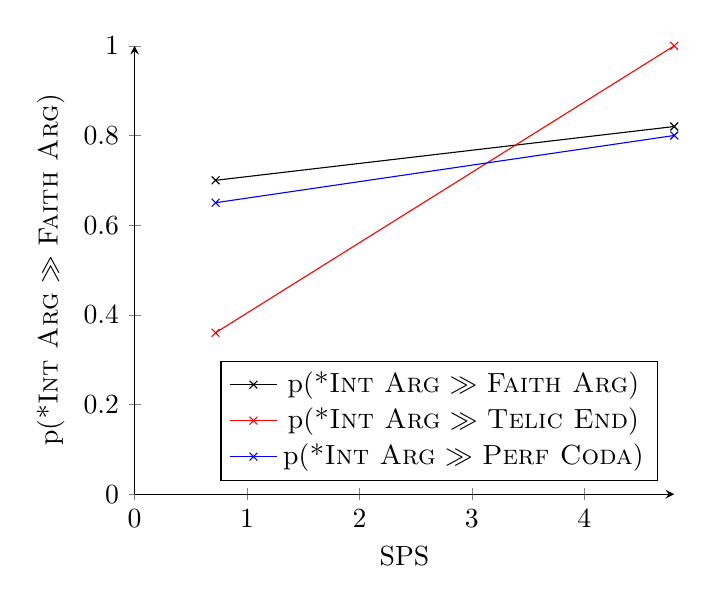
\begin{tikzpicture}
    \begin{axis}[legend pos=south east, xmin=0, ymin=0, ymax=1, axis lines = left,scaled ticks=false, xlabel={SPS}, ylabel={p(\textsc{*Int Arg} $\gg$ \textsc{Faith Arg})}] 
        \addplot[color=black,mark=x] coordinates {
        (0.72,0.70) 
        (4.80,0.82) 
    }; 
      \addlegendentry{p(\textsc{*Int Arg} $\gg$ \textsc{Faith Arg})};
            \addplot[color=red,mark=x] coordinates {
        (0.72,0.36) 
        (4.80,1.00) 
    }; 
    \addlegendentry{p(\textsc{*Int Arg} $\gg$ \textsc{Telic End})};
            \addplot[color=blue,mark=x] coordinates {
        (0.72,0.65) 
        (4.80,0.80) 
    }; 
    \addlegendentry{p(\textsc{*Int Arg} $\gg$ \textsc{Perf Coda})};
    \end{axis} 
\end{tikzpicture}
\end{figure}


\begin{figure}[htb]
\caption{Representation of the relationship between semantic selectivity and the probability of an implicit object output in Medina's model, based on computed $\gamma$ and $\delta$ values (reproduction of \reffig{medina_predictedresults}).}
\labfig{medina_predictedresults_new}
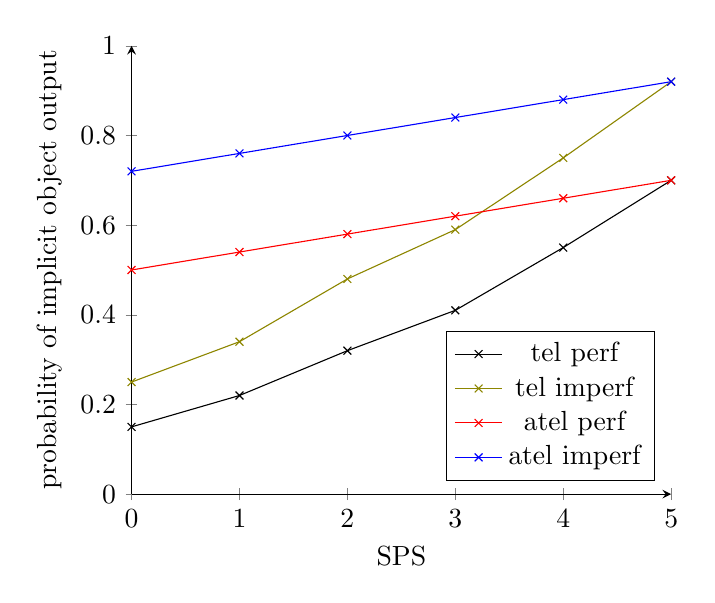
\begin{tikzpicture}
    \begin{axis}[legend pos=south east, xmin=0, ymin=0, ymax=1, axis lines = left,scaled ticks=false, xlabel={SPS}, ylabel={probability of implicit object output}] 
        \addplot[color=black,mark=x] coordinates {
        (0,0.15) 
        (1,0.22) 
        (2,0.32) 
        (3,0.41) 
        (4,0.55) 
        (5,0.70) 
    }; 
      \addlegendentry{tel perf};
        \addplot[color=olive,mark=x] coordinates {
        (0,0.25) 
        (1,0.34) 
        (2,0.48) 
        (3,0.59) 
        (4,0.75) 
        (5,0.92) 
    }; 
      \addlegendentry{tel imperf};  
        \addplot[color=red,mark=x] coordinates {
        (0,0.50) 
        (1,0.54) 
        (2,0.58) 
        (3,0.62) 
        (4,0.66) 
        (5,0.70) 
    }; 
      \addlegendentry{atel perf};    
        \addplot[color=blue,mark=x] coordinates {
        (0,0.72) 
        (1,0.76) 
        (2,0.80) 
        (3,0.84) 
        (4,0.88) 
        (5,0.92) 
    }; 
      \addlegendentry{atel imperf};        
    \end{axis} 
\end{tikzpicture}
\end{figure}

The same results I obtained in my basic model with semantic selectivity computed via Resnik's SPS are reported here in \reffig{eng_basic_sps_alltogether} and \reffig{eng_basic_sps_aspectualtypes}.


\begin{figure}[htb]
\caption{Probability of \textsc{*Int Arg} being ranked above each of the other constraints, varying in accordance with Behavioral PISA (English full model).}
\labfig{eng_basic_sps_alltogether}
    \input figures/eng_basic_sps_prob_alltogether.tex
\end{figure}

\begin{figure}[htb]
\caption{Probability of an implicit object output for each aspectual type, as a function of Behavioral PISA (English full model).}
\labfig{eng_basic_sps_aspectualtypes}
    \input figures/eng_basic_sps_prob_aspectualtypes.tex
\end{figure}

As is made evident by comparing \reffig{medina_intargabove_new} and \reffig{eng_basic_sps_alltogether}, my SPS-based basic model fails to reproduce Medina's findings. In Medina's model there is a prominent interaction between the probability of \textsc{*Int Arg} outranking \textsc{Telic End} and the probability of it outranking the two other constraints at play (i.e. \textsc{Faith Arg} and \textsc{Perf Coda}), while this interaction is absent from my SPS-based model. In particular, the relative re-ranking probabilities are ordered the same way in both models when Resnik's SPS (raw in Medina's plot, normalized in mine) is very low, i.e. \textsc{*Int Arg} is most likely to outrank \textsc{Faith Arg}, then \textsc{Perf Coda}, then \textsc{Telic End}. However, while in my model this relation also holds for high values of SPS, in Medina's model \textsc{*Int Arg} becomes more likely to outrank \textsc{Telic End} than other constraints for mid-to-high values of SPS.\\
This state of affairs is reflected in the probability of licensing an implicit object output for each separate aspectual type, reported here in \reffig{eng_basic_sps_alltogether} for Medina's model and in \reffig{eng_basic_sps_aspectualtypes} for my SPS-based basic model. Indeed, while in both models the object-dropping probabilities for the four aspectual inputs are ordered the same way for low-SPS verbs (atelic imperfective $\gg$ atelic perfective $\gg$ telic imperfective $\gg$ telic perfective), in Medina's model telic imperfective inputs are actually more likely to drop their object than atelic perfective inputs for mid-to-high-SPS verbs. In my model these probabilities vary according to SPS, but they never interact with one another.\\
However, it is interesting to note that I reproduced Medina's findings in my basic model using Computational PISA and, a bit worse, in my basic model using Behavioral PISA. I will not report here the four figures to avoid cluttering these pages, but the interested reader can compare Medina's figures with my own ones relative to the Computational PISA model (\reffig{eng_models_basic_cpisa_alltogether} and \reffig{eng_models_basic_cpisa_aspectualtypes}) and to the Behavioral PISA model (\reffig{eng_models_basic_bpisa_alltogether} and \reffig{eng_models_basic_bpisa_aspectualtypes}), collected in \refapp{app_models}. Since Medina considered a different set of verb than I did, and recruited 15 different participants than the 30 ones who participated in my experiment, it is possible to conclude that the grammar of English with respect to object drop defined by Medina is indeed true to the way native speakers of English re-rank the constraints to judge the grammaticality of object drop in their language. Crucially, Medina's results are not an artifact of the specific verbs she picked (the same as in \textcite{Resnik1993, Resnik1996}, for evident computational reasons). Why are her findings reproduced quite closely by my PISA-based basic models but not by my SPS-based basic model, which after all uses the very same measure of semantic selectivity Medina used? I would motivate these results by making reference to the shortcomings of Resnik's SPS, which I discussed extensively in \refsec{predictor_sps}, and in particular to its need for both a taxonomy (such as WordNet) and for a corpus (to extract the frequencies needed in the computation, as in \refsec{resnik_sps}). It is thus unsurprising that a model making use of a taxonomy-based measure yields results of fleeting reproducibility, even more so considering that the corpus upon which Resnik and Medina based their calculations (the Brown corpus) is much smaller than the one I employed to obtain Computational PISA scores (the ukWaC corpus).


\subsection{On regression models} \labsec{concl_lmem}

I would finally like to echo \posscite{Medina2007} concerns about the possibility of using a statistical regression model as a linguistically-informed model of language. In her thesis \parencite[132-133]{Medina2007}, she concluded that her Stochastic Optimality Theoretic model shares the property of additivity with linear regression models, since the former models the probability of an implicit object output as the sum of the probabilities of the relevant constraint re-rankings, while the latter models it as the sum of weighted variables. The main difference between the two kinds of model lies in the fact that the linguistic model keeps the input, the constraints, and the constraint re-rankings explicit, while in a regression model they are collapsed into weighted variables.\\
I second Medina's conclusions, based on the results I obtained in my own study (refer back to \refch{results} for the linear regressions and to the current Chapter for the linguistic models). In particular, I am going to compare the linear mixed-effects model\sidenote{Which, I will remember, is simply a linear regression model taking both fixed and random effects into account.} in \reftab{eng_lmem_bpisa} for English and in \reftab{ita_lmem_bpisa} for Italian with the results of my full linguistic model of object drop in \reffig{eng_ext2_bpisa_aspectualtypes} for English and in \reffig{ita_ext2_bpisa_aspectualtypes} for Italian. The mixed models clearly capture the main aspects of the linguistic models, e.g. the prominent role of telicity and perfectivity in jointly determining the grammaticality of the implicit object construction and the statistically less relevant effect of manner specification and iterativity. The role of Behavioral PISA determines another major divide between the two kinds of model, since in the regression it is assigned a weight just like any other predictor, be it continuous or binary, while in the Stochastic Optimality Theoretic model it is used as the independent variable in the computation of separate re-ranking functions for each constraint at play.\\
It is worth noting that Medina's model makes explicit use of a tenet of regression models, i.e. the requirement for the model to minimize the Summed Squared Error, which the reader can find in Medina's formulation in \refpage{medinaexcelsolver} (and again in \refsec{stot_full_fitting}) and in a more mathematically intense fashion in \textcite[13]{r_lmer} with regards to linear mixed-effects models. In a sense, a theoretical and computational method bridging the gap between linear regressions, which are linguistically naive, and Medina's model, which is not thoroughly defined as a linguistically-informed regression model, is Linear Optimality Theory \parencite{Keller2000, Keller2006}, a stochastic variant of Optimality Theory which represents the constraint rankings as numerical weights and has the grammaticality of any linguistic structure be proportional to the sum of the weights of the constraints it violates.


\pagelayout{wide} % No margins
\addpart{Conclusions}
\pagelayout{margin} % Restore margins
% \setchapterimage[6.5cm]{seaside}
\setchapterpreamble[u]{\margintoc}
\chapter{Conclusions and open questions}
\labch{conclusions}

\section{Final comments} \labsec{end_discussion}

\subsection{Recap of main findings}

I presented my models of the implicit indefinite object construction in English and in Italian in \refch{model}, together with a discussion of their performance and results. Here I will provide a short summary of the main findings of the two full models, namely, the five-predictor models I computed using Behavioral PISA (introduced in \refsec{behavPisa}) to quantify semantic selectivity, as explained in \refsec{intro_models}.\\
In general, the models perform comparably well, explaining almost half of the variance in the data (adjusted R\textsuperscript{2} is 0.468 for the English model and 0.455 for the Italian model, as reported in \refsec{intro_evaluation}). As I argued in \refch{model}, the better performance of the English model with respect to the Italian model may depend on semantic differences between the target verbs included in the behavioral experiments, and also on a more clear-cut role the predictors play in English than in Italian. These results, especially in the light of the fact that the full models improve on the performance of the reduced models (namely, Medina's three-predictor model and my own four-predictor model not considering manner specification\sidenote{As discussed in \refsec{intro_models}, the four-predictor models include Medina's three predictors and iterativity, while manner specification is only added in the full five-predictor models.}), are indeed encouraging. However, even the full models fall short of explaining all the variance in the data, demonstrating that there is still room for improvement. In \refsec{end_future}, I will propose some ideas to expand upon these models and improve their computation in future research.\\
Let us look more closely at the constraint re-rankings and subsequent grammaticality predictions of object drop in the two models. Both in English and in Italian, the probability of \textsc{*Int Arg} outranking \textsc{Telic End}\sidenote{Required to have grammatical implicit indefinite objects with telic verbs, as explained in \refch{medina} and \refch{model}.} varies strongly depending on Behavioral PISA, so that the curves described by the functions associated to this probability in the two languages are the steepest among all the curves associated to the re-ranking probabilities (as shown in \refsec{stot_full_parameters}). However, while in English the probability of \textsc{*Int Arg} outranking \textsc{Telic End} is directly proportional to semantic selectivity, in Italian the relation is one of inverse proportionality, for reasons discussed while commenting \reffig{ita_bpisa_telicity}.\\
Moreover, while in both languages the probability of \textsc{*Int Arg} outranking \textsc{Telic End} varies greatly depending on Behavioral PISA, there are differences with respect to the other predictors in the two languages. In particular, in English there is an interaction between the functions associated with the re-ranking probabilities of \textsc{Telic End} and \textsc{Perf Coda}, because telic imperfective verbs are more likely to drop their object than atelic perfective verbs for high Behavioral PISA values, while the opposite holds for Behavioral PISA scores lower than 0.8, approximately. In Italian, instead, there is an interaction between the function associated to the re-ranking probability of \textsc{Mann-Spec Arg} and the functions associated to the re-ranking probabilities of all the other constraints\sidenote{The interaction with \textsc{Non-Iter Arg} is trivial, because it happens when Behavioral PISA is 1, i.e., the maximum value.}. Thus, both models show a main effect of telicity on the probability that the object-less use of a transitive verb is considered grammatical, but the second most relevant factor in the model is perfectivity in English and manner specification in Italian.\\
In addition to the adjusted R\textsuperscript{2} values and the main role played by telicity, the two models are also comparable for:
\begin{itemize}
    \item the range of predicted object-dropping probabilities (30-100\% in English, 30-90\% in Italian);
    \item the relevance of semantic selectivity in determining the grammaticality of object drop (with re-ranking probabilities that are always directly proportional to Behavioral PISA, with the exception of \textsc{Telic End} in Italian);
    \item the fact that the predictors perform consistently with theoretical literature on object drop (refer to \refch{objectdrop}, \refch{factors}, and \refch{predictors}).
\end{itemize}

Indeed, in both models atelic imperfective iterative manner-specified verbs are the most likely to drop their object (between 80\% and 90\%), while telic perfective non-iterative manner-unspecified verbs are the least likely (between 30\% and 40\%). Moreover, atelic verbs are more likely to occur with implicit objects than telic verbs, imperfective verbs more than perfective verbs, iterative verbs more than non-iterative verbs, and manner-unspecified verbs more than manner-specified verbs, as expected.\\
Even though semantic selectivity plays an active role in both models, the range of predicted grammaticality across different input types is not the same in English and in Italian. Indeed, while it is comparable for low-Behavioral PISA verbs in the two languages (ranging from 30\% to 80\% in English and from 30\% to 90\% in Italian), it is much narrower and higher in English (between 90\% and 100\%) than in Italian (between 40\% and 90\%), as shown and discussed in \refsec{stot_full_predicted}.


\subsection{Comments on iterativity and manner specification}

In this dissertation, I modeled the implicit indefinite object construction following \posscite{Medina2007} steps. A major element of novelty I added is the inclusion of two novel constraints in the model, i.e., \textsc{Non-Iter Arg} and \textsc{Mann-Spec Arg} (refer to \refch{model}), which are based on the role played by iterativity and manner specification (refer to \refch{factors}), respectively, in facilitating indefinite object drop.\\
As I argued in \refsec{intro_evaluation}, the addition of these two new constraints proved to be beneficial to the performance of the model when applied both to English and to Italian data. Indeed, the full five-predictor models explain the variance in the data better than the three- and the four-predictor models regardless of the chosen measure of semantic selectivity (Resnik's SPS, Computational PISA, or Behavioral PISA). However, the four-predictor models (including iterativity in addition to Medina's telicity, perfectivity, and semantic selectivity) do not perform better than the three-predictor models, with basically identical adjusted R\textsuperscript{2} values in English and slightly smaller adjusted R\textsuperscript{2} values in Italian. Taken together, these results mean that iterativity alone is not a sufficient addition to Medina's model (rather, it makes the model needlessly more complicated, since it does not explain more variance in the data), but models including iterativity and manner specification together have a stronger explanatory power.\\
The lower performance of the models including iterativity without manner specification echoes observations drawn in \refsec{stot_full_parameters} relative to the probability of \textsc{*Int Arg} outranking \textsc{Non-Iter Arg}, that was shown to be very high both in a relative sense (since it is the highest among all the re-ranking probabilities) and in an absolute sense (92-100\% in English, 96-100\% in Italian). Since \textsc{Non-Iter Arg} is vacuously satisfied by iterative inputs, and varies almost imperceptibly according to semantic selectivity with non-iterative inputs (for which it is an active constraint), it stands to reason that it has no noticeable effect on the predicted grammaticality of object drop.\\
The same analysis would also explain the significant effect of the full models, where manner specification is also included among the predictors. In particular, in \refsec{intro_evaluation} I showed that the addition of manner specification determines a much stronger qualitative leap in the full models of Italian than in English, where the increase in the performance of the models is rather modest. Once again, these results are related to the probability of \textsc{*Int Arg} outranking the relevant constraint, i.e., \textsc{Mann-Spec Arg}. As shown in \refsec{stot_full_parameters}, the curve described by the function associated to this re-ranking probability is quite steep in Italian and it intersects all the other curves, while in English it is not steep at all and it has no interactions with the other curves. Thus, manner specification in Italian interacts in meaningful ways with semantic selectivity (as shown by the steepness of the curve) and the other binary predictors of object drop, making it an important factor in an expanded model of indefinite object drop. In English it has an effect too, but less evident.


\subsection{Comments on semantic selectivity}

In addition to the presence of additional constraints in the models, the other dimension of variation highlighted in \reftab{tab_mymodels} in \refsec{intro_models} is the measure used to quantify semantic selectivity in the models. In particular, I computed three families of models, each based on Resnik's SPS (as in Medina's original model), on Computational PISA, or on Behavioral PISA. In \refsec{intro_evaluation}, I provided adjusted R\textsuperscript{2} scores of each model in each family, showing that in English SPS-based models are the worst-performing, while PISA-based models are noticeably better (with Behavioral PISA being better than Computational PISA). In Italian, instead, Computational PISA-based models are the worst-performing, followed by SPS-based models and, lastly, by Behavioral PISA-based models.\\
In \refch{model}, I provided a possible explanation of these facts, together with the correlations between semantic selectivity and average Likert grammaticality ratings presented in \refsec{eng_judgresult_semsel} and \refsec{ita_judgresult_semsel}, by making reference to the way each measure of semantic selectivity is defined and computed (as detailed in \refsec{predictor_sps}). Let us consider the different performance of the three families of models in the light of \refsec{evalMySPSs}, where I evaluated the correlations between the three measures of semantic selectivity both in English and in Italian. I argued that the English facts (SPS-based models being worse than PISA-based models, and SPS correlating poorly with PISAs while Behavioral PISA and Computational PISA correlate well with each other) may depend on the nature of these measures, considering that both PISA measures are based on the computation of pairwise similarity scores (distributional cosine similarity for Computational PISA, Likert-scale human judgments of similarity for Behavioral PISA), while SPS suffers from all the problems of taxonomy-based measures, as discussed in \refsec{predictor_sps}. The Italian picture is different, since in this case Computational PISA-based models perform worse than SPS-based models. Interestingly, as shown in \refsec{ita_judgresult_semsel}, Computational PISA in Italian correlates very well with SPS (even better than with Behavioral PISA). I take this to mean that even after the manual cleansing I performed to purge any artifacts from the corpus data (recounted and motivated on \refpage{cleanthecorpus}), the itWaC corpus, upon which I based the computation of SPS and Computational PISA relative to Italian, has a stronger effect on the resulting scores than the ukWaC corpus, which I used to model the computational measures of semantic selectivity in English.\\
However, there may also be some undesirable side effect generated by the choice of ukWaC for English, given that I was able to reproduce Medina's findings relative to indefinite object drop in English with my three-predictor PISA-based models, but not with SPS, which is the measure she used (refer to \refsec{concl_medinacompare}). This may depend either on the corpus of choice or on the set of target verbs (or on both), but I am confident I can take the verbs off the suspect list because I made sure to include strictly transitive, as much as possible monosemous, verbs in my set (refer to \refsec{verbs}), while Medina used the same verbs included in \posscite{Resnik1993} original computation of SPS, a set including also verbs such as \textit{to do, to get, to have}. Thus, I conclude that I was not able to reproduce Medina's model using SPS because of the corpus I used. It would be possible to test this hypothesis by computing again Medina's model using her verb set and ukWaC, and my verb set and the corpus Resnik (and thus Medina) based his computation on. % If my hypothesis is correct, I would not replicate Medina's results in the former scenario, but I would do so in the latter. Of course, one may argue that the fault in the lack of replication may well lie in Medina's model itself, namely, either in her computation of SPS, or in artifacts determined by her choice of target verbs (which may be poor representatives of optionally transitive verbs in English). However, she based her analysis on Resnik's verb set and SPS scores, and it would be very improbable indeed that the inventor of SPS himself miscalculated his own model of object recoverability. The verbs would be a more likely culprit, but, on the other hand, I was able to replicate Medina's results with my PISA-based three-predictor models. How could Medina's model be wrong, but also consistent with a model of object drop (and, consequently, of the grammar of the English language) based on a different measure of semantic selectivity and different target verbs? Clearly, this scenario would be most unlikely.\\
To conclude, I observe that both in English and in Italian the best-performing models are based on Behavioral PISA. This result does not surprise at all, since this measure, being based on human similarity judgments, can be considered a benchmark model for semantic selectivity.


\section{Future directions} \labsec{end_future}

\subsection{Expanding the model} \labsec{expandingthemodel}

\paragraph{Additional predictors}

Among the linguistic factors facilitating indefinite object drop presented in \refch{factors}, I only picked five to serve as predictors in my models (detailed in \refch{predictors}), namely: semantic selectivity, telicity, perfectivity (all three from \posscite{Medina2007} original model), manner specification, and iterativity (two novel additions), for reasons detailed in \refsec{factorsofchoice}. The way these predictors are implemented in the (linear) Stochastic Optimality Theoretic models was explained in \refch{medina} relative to Medina's model and in \refch{model} relative to mine.\\
Future research may expand upon my models in the same way I expanded upon Medina's, namely, by introducing additional predictors in the model based on theoretical literature. A relevant area of interest, which I only brushed against by including iterativity (a broadly-intended pragmatic factor) in my model, is that of pragmatic and discourse factors (refer to \refsec{pragmaticfactors}). Since out-of-context utterances only happen in laboratory environments, research on pragmatic and discourse factors will provide much more ecological data to studies on indefinite object drop. However, this should not be intended as a potshot at models based on no-context stimuli, such as Medina's and the ones proposed in this dissertation. Indeed, given that the same semantic and aspectual factors determine indefinite object drop both in context-rich and in no-context utterances, it makes sense to model these factors first and to add contextual factors later on. Moreover, a word of caution is needed regarding the possible addition of pragmatics to experiment on indefinite object drop, since sufficient context may make virtually any object recoverable and, thus, any transitive verb acceptable when used intransitively. Thus, experiments including intra- and extra-linguistic contexts will have to be carefully calibrated in order to quantify the exact role of each type of context, and to avoid having context-external factors confound the experiment.\\
Given that indefinite object drop challenges prototypical transitivity, it would also be interesting to include in the model the neglected parameters described by \textcite{HopperThompson1980} (refer back to \reftab{ht1980_parameters} in \refsec{theory_transitivity}), in particular affirmation, mode, agency (strictly related to Agent affectedness, discussed on \refpage{affectedagent} and in \refsec{agentaffect}), and affectedness of the object (tackled in \refch{objectdrop}).

% PM: aggiungerei che i fattori pragmatici devono essere attentamente calibrati. In contesto, qualunque cosa può essere sottintesa purché inferibile. Ciò vale anche per gli argomenti che in esperimenti controllati risultano incancellabili.
% Quindi limiterei un po' il ruolo della pragmatica; è vero che potenzialmente può aggiungere qualcosa, ma come se ne misura l'effetto?

\paragraph{Corpus frequencies}

As shown in \textcite{Boersma2004, BoersmaHayes2001empirical}, Stochastic Optimality Theory can be used to model corpus data just as well as grammaticality judgments, namely, via the evaluation of constraints that get re-ranked along a continuous numerical scale (refer to \refch{modeltheory}). Rather than trivially duplicating the results I obtained and discussed in this dissertation, new models of corpus frequencies are sure to shed a different light on the implicit indefinite object construction. As I anticipated in \refsec{frequencyfail}, neither \textcite{Resnik1993, Resnik1996} nor \textcite{Medina2007} found a precise correlation between corpus frequencies and the gradient grammaticality judgments provided in behavioral experiments about implicit indefinite objects.\\
Indeed, linguistic research has long since shown that there is no clear-cut correspondence between ratings elicited from native speakers and corpus frequencies \parencite{manning2003probabilistic}. In particular, it is often the case that low-frequency utterances (or other linguistic items) receive mid-to-high acceptability judgments in behavioral experiments \parencite{KempenHarbusch2005, BermelKnittl2012, BaderHaussler2010, Boersma2004, KellerAsudeh2002}. There is also no strict relation between the relative grammaticality of a linguistic structure with respect to another and their relative corpus frequencies, since, for instance, \textcite[315-316]{BaderHaussler2010} report that they found no pairs of syntactic structures in their study where a member of the pair was judged as more grammatical than the other but occurred with a smaller frequency in the corpus, while \textcite{Boersma2004} argues in favor of the opposite. Moreover, \textcite{BaderHaussler2010} experimental results show both a "ceiling mismatch"\sidenote{The authors also observe that this is not a measurement artifact due to the use of a capped scale, such as binary or 7-point Likert ratings, because it is also found with Magnitude Estimation ratings, which are open-ended both at the top and at the bottom.} (meaning that two syntactic structures may be judged as maximally grammatical, but occur with different frequencies in the corpus) and a "floor mismatch" (meaning that two syntactic structures may never or almost-never occur in the corpus, but receive different acceptability judgments).\\
A common worry about linguistic research based on corpus material is that frequencies are less reliable than human judgments because there is no way to control language production as one controls an experimental design. This line of reasoning would surely curb easy enthusiasm about the replication of the current study to model corpus frequencies of indefinite object drop, if \textcite{Steube2008, Schutze2016} did not observe that acceptability ratings are too "contaminated by performance factors", that is to say, biased by other tasks the raters perform in addition to the one they are explicitly asked to carry out (e.g., they judge the similarity between the target sentence and the one they consider its "ideal delivery" paraphrase). Thus, if linguistics gladly relies on acceptability judgments (and, oftentimes, the results of one's own introspection), provided they are based on a rigorous experimental design, there should be no qualms about modeling corpus frequencies, provided they are interpreted in the light of the factors possibly influencing them. In general, given that no experimental method is error-free, it is good practice to compare the results obtained with different methods. In the specific case of studies on indefinite object drop, there may be a trade-off between the analysis of easily computable\sidenote{Provided the corpus is annotated in such a way as to make data extraction easy, of course.} frequencies extracted from non-manipulable\sidenote{Also, possibly under-representative of the language one intends to study, given that even in corpora that are not genre-specific it is difficult to obtain complete coverage of language uses and contexts.} corpus utterances, and the analysis of acceptability judgments provided by human subjects on easily manipulable experimental stimuli, even though these judgments stem from often unfathomable individual processes going on in the mind of each subject.\\
Modeling corpus frequencies of indefinite null objects using the very same model(s) defined in this dissertation may present additional challenges if compared to modeling acceptability ratings, since it is impossible to manipulate aspectual and discourse factors in a corpus study as in a behavioral experiment. However, the possible absence (or very low frequency) of a given object-less verb in a given aspect may well be considered an interesting, modelable datum in itself, provided one adjusts the model to account for such findings. Alternatively, it would be possible to design a production experiment to design an \textit{ad-hoc} corpus to model the frequency of indefinite null objects in controlled speech or writing. It is also important to note that it would be possible, if not even easy, to include discourse and world-knowledge context (somewhat ancillary to semantics and aspectual factors in this dissertation) in a model of object drop based on frequencies extracted from a large corpus, given that these null objects appear in sentences which are part of larger documents with explicit context information. Moreover, a corpus study of object drop may provide an answer to a question foreshadowed by \textcite{KempenHarbusch2005, Medina2007} (refer to \refsec{frequencyfail}), namely, whether a "production threshold" exists blocking mid-to-low grammaticality structures from ever being uttered and, if so, which numerical value has to be assigned to this threshold.

% PM: aggiungerei che, siccome nessun metodo sperimentale è privo di intrinseci limiti, è buona prassi confrontare i risultati di diversi metodi.
% Nel caso specifico, si può ipotizzare un trade-off fra la rigidità dei contesti fissati nei corpora, e l'inverificabile libertà individuale nel ricostruire mentalmente i possibili contesti d'uso in relazione agli stimoli.

% AL: Il problema non è solo quello. C’è la distribuzione zipfiana dei dati anche la difficile valutazione della rappresentatività dei dati. Last but not least i problemi della loro estrazione

\paragraph{Other implicit complements of verbs}
Direct object of optionally transitive verbs are far from being the only NP complements of verbs participating in syntactic omissions. For instance, the literature mentions:

\begin{itemize}
    \item Agents of passives, as in \textit{The ship was sunk $\varnothing$\textsubscript{Agent}} \parencite{BhattPancheva2017implicit, Lasersohn1993, RuppenhoferMichaelis2014};
    \item Source \parencite{Gillon2006english}, Goal \parencite{Lasersohn1993, RuppenhoferMichaelis2014}, and Path \parencite{recanati2002unarticulated} locative phrases occurring with motion verbs\sidenote{Interestingly, \textcite[9-12]{Gillon2006english} and \textcite[333]{ruppenhofer2011search} observe that in some pairs of near-synonym verbs, such as \textit{to leave, to vacate} and \textit{to arrive, to reach}, only one member of the pair allows for the omission of the locative phrase. This is consistent with the literature on the role of manner specification in argument omission (refer to \refsec{mannerspec}).}, as in \textit{Bill left $\varnothing$\textsubscript{Source}}, \textit{Hilary arrived $\varnothing$\textsubscript{Goal}}, and  \textit{The cow jumped over $\varnothing$\textsubscript{Path}};
    \item Themes of reflexive (\textit{Peter shaved (himself)}) and reciprocal (\textit{Mary and Peter divorced (from each other)}) predicates \parencite{NemethEniko2014};
    \item Recipients of three-argument verbs, as in \textit{The mayor donated \$300 $\varnothing$\textsubscript{Recipient}} \parencite{ruppenhofer2005regularities};
    \item Instruments, as in \textit{The executioner beheaded the prisoner $\varnothing$\textsubscript{Instrument}} \parencite{KoenigEtAl2002, KoenigEtAl2003, KoenigEtAl2007, RissmanEtAl2015, RissmanRawlins2017, Rissman2010}.
\end{itemize}

Among all these \textit{syntactically} optional complements of verbs, Instruments stand out because they can also be \textit{semantically} optional. Indeed, \textcite{KoenigEtAl2002, KoenigEtAl2003, KoenigEtAl2007} divided Instrument-taking verbs into two classes, i.e., the Require-Instrument class (\textit{to chop, to slice, to write}) and the Allow-Instrument class (\textit{to eat, to break, to open}). In \textcite{CappelliLenciPISA}, I computed Computational PISA scores of Instrument-taking English verbs (together with transitive verbs, as discussed in \refsec{compuPisa}), showing that this measure of semantic selectivity can reliably tell apart Require- and Allow-Instrument verbs. I argue that this is a promising starting point in a possible computational model of the factors regulating the syntactic optionality of Instruments, given the insight this method provided in the study of indefinite object drop.\\
Modeling Instruments, as well as the other implicit complements listed in this Section, will provide useful information to further theoretical and experimental research on syntactic optionality.

\paragraph{Indefinite object drop diachronically}
As argued in \refsec{frequencyfail}, with reference to \textcite{Goldberg2001, Goldberg2005a, Lorenzetti2008, Glass2020}, verbs appearing in generic contexts with a habitual interpretation (e.g., \textit{Pat drinks; Pat smokes; Chris sings; Sam bakes}, from \textcite[518]{Goldberg2001}) are likely to participate in the implicit indefinite object construction, due to Goldberg's principle of Omission under Low Discourse Prominence. Diachronically, the frequent use of transitive verbs in such contexts probably led to the grammaticalization of their intransitive use in episodic contexts as well, often with a specialized meaning (e.g. 'to drink alcohol' in \textit{Pat drinks}, 'to bake pastries' in \textit{Sam bakes}).\\
A model of indefinite object drop in historical and contemporary texts (a gap in the literature first observed by \textcite{Goldberg2001}) would substantiate this hypothesis and shed some more light on the mechanisms regulating the role of semantic and aspectual predictors in addition to discourse factors. Moreover, diachronic change also affects semantic selectivity (which, as discussed in \refch{objectdrop}, \refch{factors}, and \refch{predictors} is a major predictor of indefinite object drop) and other facets of verb meaning. For instance, verbs may undergo semantic changes expanding the range of their meaning (e.g., Vulgar Latin \textit{*adripare} 'to reach the shore' gave rise to Italian \textit{arrivare} 'to arrive'), shifting it from a concrete to a metaphorical interpretation (e.g., \textit{to broadcast} originally meant 'to cast seeds widely' on a field, while the rise of communication technologies in the 20th century shifted its meaning to 'spread a message or news widely'), or restricting it (e.g., Latin \textit{cubare} 'to lie, to rest' became Italian \textit{covare} 'to brood', referring to the lying act performed by egg-laying animals to nurse their eggs).\\
Several corpora of English and Italian are available for a diachronic study on indefinite object drop, each focusing on different text types within different time spans. Among the diachronic corpora of English\sidenote{Refer to \textcite{hilpert2016quantitative} for an introduction to quantitative approaches to diachronic corpus linguistics mentioning several corpora of English.}, relevant ones to inquire about null objects may be:
\begin{itemize}
    \item the Helsinki Corpus of English Texts \parencite{rissanen1993helsinki}, spanning over Old (V-XII centuries) to Early Modern (late 15th - late 17th centuries) English, and covering many different genres (such as chronicles, handbooks, laws, and Bible excerpts);
    \item the Corpus of Late Modern English Texts \parencite{deSmet2005corpus, deSmet2015corpus}, covering public domain British English texts from 1710 to 1920;
    \item the Corpus of Historical American English \parencite{davies2010corpus, davies2012expanding}, recently purged of inconsistent lemmas and malformed tokens \parencite{alatrash2020ccoha}, a large-scale (around 400 million words) corpus covering different genres (newspapers, fiction and non-fiction books, magazines) from 1810 to 2009.
\end{itemize}

As for Italian, relevant diachronic corpora may be:
\begin{itemize}
    \item DiaCORIS \parencite{onelli2006diacoris}, a 100-million-word corpus of texts written between 1861 (year of the National Unification) and 1945 covering genres such as newspapers, fiction, and academic prose;
    \item the MIDIA corpus \parencite{gaeta2013midia, iacobini2014midia}, a 7-million-word corpus of documents written between the 13th and the 20th centuries;
    \item the OVI corpus \parencite{ovi2005corpus}, a half-million word corpus of texts from the 12th to the 14th centuries;
    \item a diachronic corpus of newspaper articles published on "L'Unit\`{a}", the official newspaper of the Italian Communist Party from 1924 to the dissolution of the Party in 1991, published between 1924 and 2015.
\end{itemize}

In theory, the wider the time span covered by a given diachronic corpus, the better. A corpus ranging over several centuries of written language would indeed provide a broad perspective on the possible grammaticalization of null objects outside habitual contexts. However, it may also be the case that changes in grammar happened much faster in the last century, when distant communication became possible, literacy was not an upper-class privilege anymore, and, in the last 30 years or so, English became the main language of the internet. As for Italian, \textcite{basile2020diachronic} observe that deep changes occurred in this language during the second half of the 20th century. Thus, it is possible that use-dependent pressures towards the grammaticalization of null objects are more evident in corpora focusing on the last century, than on previous time periods. Moreover, subtle changes of this kind are surely more frequent and observable in corpora based on spoken language, or language written to be read shortly after (such as the one used in newspapers and other mass media). Thus, both broad diachronic corpora and 20th-century corpora may be of use to understand the history of indefinite object drop.

% PM: ottima prospettiva di ricerca; qui completerei il discorso indicando su quali corpora inglese e italiani si potrebbe condurre una simile ricerca diacronica, e con quali limiti eventuali dovuti al tipo di testi.
% Quest'ultima cautela potrebbe semplicemente essere espressa come un fatto da tenere in considerazione.

% AL: Potresti menzionare anche il fatto che i. Diacronia ca,bua anche il senso dei verbi e a che la loro se,antic selectivity. Pensa al famoso caso di adripare che significava andare su un’altra riv del fiume e poi ora significa arrivare in qualsiasi luogo. I processi di restringimento o allargamento semantico possono produrre effetti sulla semantic selectivity e dunque sull’omissione dell’oggetto

\paragraph{Typologically different languages}
In this dissertation, I modeled the implicit indefinite object construction in English and Italian, two typologically close languages. As discussed in \refch{model}, several differences between the two emerged with respect to their licensing of indefinite null objects, meaning that this phenomenon depends on much finer-grained aspects than what typology alone would warrant. Nevertheless, a theory of grammar should not be a theory of English and English-like languages alone, and therefore a comprehensive model of indefinite object drop should consider a variety of typologically different languages.\\
As noted by \textcite[134]{Jackendoff2003}, languages such as Korean and Japanese (to which we may add Chinese) allow for null arguments more easily than English, so that they would pose "no justification for distinguishing between obligatorily and optionally expressed semantic arguments". However, in the same paragraph he also argues in favor of the distinction between definite and indefinite null objects being a fully idiosyncratic lexical property of verbs or, at most, of semantic verb classes, a position which I argued against throughout \refch{objectdrop} and \refch{factors}. Thus, it is not to be excluded that languages such as Korean, Japanese, and Chinese may show different degrees of acceptability of indefinite object drop with different optionally transitive verbs, even if they are free in their Topic-drop-based licensing of definite null objects (just like English and typologically similar languages are, as argued on \refpage{recipes}). Another aspect differentiating these languages from languages such as English and Italian, with respect to aspects playing a role in object drop, is their treatment of non-culminating accomplishments. Indeed, while in English the sentence \textit{*I burned it but it didn't burn} is utterly ungrammatical due to being contradictory, its Japanese equivalent (\textit{moyashita keredo moenakatta}, as reported in \textcite[236]{radden2003metonymic}) is grammatical because the verb \textit{moyasu} 'to burn' is less focused on the result than its English counterpart \textemdash it is, thus, a non-culminating accomplishment. The existence of such verbs made \textcite{ikegami1991language} distinguish between DO-languages such as English, focusing on the Agent, and BECOME-languages such as Japanese, focusing on the process. Indeed, given the considerations provided in \refsec{theory_incorporation} relative to indefinite object drop as a mechanism driven by the need to focus on the activity rather than on its effects on the Patient, it stands to reason that BECOME-languages should allow object drop more often and in a wider variety of contexts than DO-languages.\\
Another typologically different family, namely, Slavic languages, may shed light on the role played by grammatical aspect in the implicit indefinite object construction. As mentioned in \refsec{perfectivity}, simplifying a very long tradition of studies in a way that will surely disgruntle many of those who fostered research in this area, in Slavic languages perfectivity is embedded in the lexicon rather than being expressed morphologically (as in English and Italian). To be more precise, in Slavic languages the opposition between so-called perfective and imperfective verbs actually derives from the encoding (or lack thereof) of telicity in the verb \parencite{bertinetto2012diachronic, bertinetto-delfitto2000aspect, bertinetto2001frequent}. In a diachronic perspective, discussed in \textcite{bertinetto2012diachronic} relative to Russian, the loss of the overt aspectual markers in the passage between Old Slavonic to (Northern) Slavic languages gave rise to a syncretic system merging lexical aspect and grammatical aspect. The opposition between prefixed and simple verbs in Russian is interpreted as "unmistakable evidence" of the original distinction being one of lexical, not grammatical, aspect. Crucially, since so-called imperfective Slavic verbs can be used in perfective contexts, and given that so-called perfective verbs are always ungrammatical with null objects \parencite{sopata2016null, TsimpliPapadopoulou2006}, experiments relative to indefinite object drop in Slavic languages (be they corpus-based or judgment-based) should only focus on the realization of implicit objects with imperfective transitive verbs. I take this state of affairs to mean that \textsc{Perf Coda} acts as a hard constraint in Slavic languages, being always re-ranked above \textsc{*Int Arg} for perfective inputs (refer to \refch{medina} and \refch{model}), instead of being a soft, re-rankable constraint as it is in English and Italian. Indeed, as discussed in \refsec{telperftense}, in these two languages telicity, perfectivity and tense are intertwined, so that the interpretation of one factor partially depends on the others. This explains why in my models telicity and (secondarily) perfectivity both play a gradient role in favoring object drop, depending on each verb's semantic selectivity, despite the behavioral experiments being carefully designed to isolate the effect of each factor at play. Based on previous considerations, I hypothesize that a model of indefinite object drop in Slavic languages would paint quite a different picture.

% PM: aggiungici il cinese; poi ne esistono tante altre, ma per questo tipo di indagine bisogna andare su lingue con ampia disponibilità di corpora.
% Comunque sia, il discorso che fai è incompleto; lo puoi completare accennando al tema dei così detti 'non-culminating telics'; nelle lingue qui citate, e in tante altre, il valore telico dei predicati è assai labile.
% Si può dire per es.:
% I burned it but it didn't burn
% (che era il titolo di una articolo sul giapponese)
% perché 'bruciare X' non significa necessariamente 'consumarlo col fuoco', ma può significare 'appiccargli il fuoco'. L'entrata lessicale è la stessa, la sua interpretazione telica varia a seconda del contesto.

% PM: te lo lascio dire così, ma è una c....ta.
% Anzi no, non te lo lascio proprio dire. 
% (a lezione dormivi, di' la verità!)
% Il problema qui non è la perfettività in quanto tale, ma la telicità necessariamente soddisfatta (in quanto lessicalmente espressa). La perfettività DISCENDE dalla telicità incorporata nel predicato.
% Difatti, i verbi slavi 'imperfettivi' possono tranquillamente essere usati in contesti perfettivi. 
% Quindi vedi bene che quasi tutti quelli che scrivono su queste cose ripetono scemenze, che si propagano di citazione in citazione.
% Maledetti!!!!

% PM: per l'appunto! Siccome nelle liingue slave l'integrazione di azionalità e aspetto è ancora più tenace, perché lessicalmente espressa (almeno per i verbi 'perfettivi'), ci si deve aspettare un diverso comportamente.
% Anzi, guarda, per quanto riguarda i 'perfettivi' transitivi è perfettamente inutile la verifica sperimentale, perché senza oggetto espresso le frasi sono banalmente inaccettabili. Ci si può solo concentrare sugli 'imperfettivi' transitivi.
% Questo almeno dillo, se no ... calci negli stinchi!

% vecchia frase mia: Should experimental evidence confirm the claim that Slavic languages do not allow for object drop with perfective verbs, this would mean [hard constraint]


\subsection{Different math}

In this dissertation I followed \textcite{Medina2007} in providing a Stochastic Optimality Theoretic model of indefinite object drop (see \refch{medina}) where the binary predictors described in \refch{predictors} are used to define four faithfulness constraints re-ranking with respect to \textsc{*Int Arg} (a markedness constraint). Semantic selectivity, modeled along a continuous numerical scale, cannot give rise to a binary constraint itself. Instead, Medina implements it in the model by defining the probability of each faithfulness constraint re-ranking with respect to \textsc{*Int Arg} as a (linear) function of the semantic selectivity of the input verb, deviating from the Stochastic Optimality Theoretic norm of associating fixed normal curves to constraints (refer to \refsec{stochot}). However, as \textcite[110]{Medina2007} herself comments, there is no compelling reason why these re-ranking functions should be necessarily \textit{linear} functions. Indeed, she argues that linear functions are "a reasonable place to begin to explore the relative contribution of
Semantic Selectivity to the implicit object construction", and I followed in her steps to obtain models comparable to hers. Future research on indefinite object drop may benefit from employing non-linear functions, defining a more complex algorithm than the one used here to determine the best function and its parameters.\\
Going back to linear Stochastic Optimality Theoretic models of object drop, in \refsec{concl_lmem} I commented on the differences between them and linear mixed-effects models, which are linear regression models including both fixed and random effects in the computation. Mixed models, by their very nature, are able to account both for the effect of the predictors of object drop on the grammaticality of indefinite null objects (the fixed effects), and for the effect of the source of random variability in the data, i.e., the target verbs and the participants to the experiment (the aptly-named random effects). Medina's model and my own, instead, are more like classic linear regression model in that they only account for fixed effects. I minimized any effect the human participants may have had on the results by modeling their normalized ratings (refer to \refsec{likert_preprocessing}), but this pre-processing adaptation of the Likert ratings is more of a quick fix than the kind of solid method I endorse for future research. Indeed, ideally the model should take raw ratings as input, and not only account for the different use the participants made of the Likert scale, but also quantify the amount of variance in the data depending on the participants alone. The same goes for random effects depending on the target verbs, which my models are not able to compute.

\subsection{A follow-up on recoverability and prototypicality}

In \refsec{whichobjects}, I argued, with reference to the literature, that indefinite null objects refer to the prototypical Patients of a given transitive verb, as recovered by speakers via world knowledge. However, this prototypicality is not to be intended as a monolith. Rather, it depends on extra- and intra-linguistic context, as it is possible to argue based on \posscite{Rice1988} examples in \ref{rice_concl}. In \ref{rice1_concl}, the act of smoking is intended to refer to cigarettes, because they are the most common object of smoking in contemporary Western society, but different context (such as a mention to olden times, or a Middle-East setting) may induce a reading where the omitted object refers to a pipe or a waterpipe. In \ref{rice2_concl}, the act of drinking is linked to alcohol assumption for reasons made clear in \refch{objectdrop} and \refsec{agentaffect}, but it would necessarily refer to some other prototype were the subject a toddler or a teetotaler, let alone a non-human participant. Similarly, John may be understood to drive a bike in \ref{rice3_concl} and to read a newspaper in \ref{rice4_concl}, provided slight differences in the available context (e.g., a downtown location to drive to, or a different reading time).

\ex. \label{rice_concl} \a. \label{rice1_concl} John smokes (cigarettes / *Marlboros / *a pipe / *SMOKING MATERIALS).
\b. \label{rice2_concl} John drinks (alcohol / *gin / *water / *coffee / *LIQUIDS).
\c. \label{rice3_concl} When he goes to Boston, John drives (a car / *a Toyota / *a motorcycle / *A VEHICLE).
\d. \label{rice4_concl} Each afternoon, John reads (a book / *Ulysses / *the newspaper / *PRINTED MATTER).

Therefore, possibly enriching some additional models I envisioned in \refsec{expandingthemodel}, it may be useful to design an experiment targeted at the prototypicality\sidenote{This task tackles a different problem than the one this thesis focused on (i.e., modeling the grammaticality of object-less transitive verbs).} intrinsic to object recoverability. I would imagine a cloze-test experiment where subjects have to fill in the gap in sentences such as \textit{John smokes \_\_\_}, manipulating context as to have no-context sentences, common-sense contexts, and uncommon contexts. I hypothesise that there would be much greater agreement between participants relative to the fillers of common-context stimuli and no-context stimuli (where the context is inherently provided via world knowledge), than the agreement relative to uncommon-context stimuli (where it is difficult to imagine prototypicality). % I suspect a reaction-time experiment relative to the acceptability of such object-less stimuli would yield results consistent with these expectations.

% AL: Questo i sembra un problema diverso da quello che hai affrontato nella tesi. Ti occupi dell’a ettabilita di frasi con oggetto omesso e non di quale oggetto viene tipicamente recuperato. Ok come prospetttiva di ricerca, ma solo se dici che è un task di tipo diverso 

\appendix % From here onwards, chapters are numbered with letters, as is the appendix convention

\pagelayout{wide} % No margins
\addpart{Appendix}
\pagelayout{margin} % Restore margins

\setchapterpreamble[u]{\margintoc}
\chapter{Verbs used in the stimuli}
\labapp{app_verbs}

This appendix collects the English and Italian verbs used in the stimuli of the behavioral experiment eliciting acceptability judgments about the implicit object construction, as explained in full detail in \refsec{verbs}.\\
These data are also available \href{https://github.com/giuliacappelli/dissertationData}{on my GitHub profile}\footnote{https://github.com/giuliacappelli/dissertationData}. The stimuli used in the behavioral experiment are listed in the same GitHub repository and here in \refapp{app_stimuli}.

\section{Target verbs}

\subsection{Matching English and Italian verbs}

\begin{longtable}{l|l}
\textbf{English}      & \textbf{Italian}    \\
\hline
\endhead
behead	&	decapitare	\\
break	&	rompere	\\
build	&	costruire\\	
chop	&	spaccare	\\
clean	&	pulire	\\
cook	&	cucinare	\\
cut	&	tagliare	\\
devour	&	divorare	\\
doodle	&	scarabocchiare\\	
drink	&	bere	\\
eat	&	mangiare	\\
embroider	&	ricamare	\\
hum	&	canticchiare	\\
kill	&	uccidere	\\
knife	&	accoltellare	\\
poison	&	avvelenare	\\
polish	&	lucidare	\\
pour	&	versare	\\
sew	&	cucire	\\
sign	&	firmare	\\
sing	&	cantare	\\
sip	&	sorseggiare	\\
slice	&	affettare\\	
smoke	&	fumare	\\
steal	&	rubare	\\
swig	&	trangugiare	\\
teach	&	insegnare	\\
wash	&	lavare	\\
watch	&	guardare	\\
write	&	scrivere  
\end{longtable}

\subsection{English}

\begin{longtable}{l|rr}
\textbf{verb}      & \textbf{frequency}    & \textbf{Zipf scores}    \\
\hline
\endhead
behead    & 1674      & 2.9418     \\
break     & 196609    & 5.0116     \\
build     & 479945    & 5.3992     \\
chop      & 15330     & 3.9036     \\
clean     & 53629     & 4.4474     \\
cook      & 36378     & 4.2789     \\
cut       & 158274    & 4.9174     \\
devour    & 3447      & 3.2555     \\
doodle    & 350       & 2.2621     \\
drink     & 56215     & 4.4679     \\
eat       & 136063    & 4.8518     \\
embroider & 2689      & 3.1476     \\
hum       & 2714      & 3.1516     \\
kill      & 140951    & 4.8671     \\
knife     & 494       & 2.4118     \\
poison    & 4710      & 3.3910     \\
polish    & 6360      & 3.5215     \\
pour      & 26960     & 4.1487     \\
sew       & 4141      & 3.3351     \\
sign      & 168608    & 4.9449     \\
sing      & 75238     & 4.5945     \\
sip       & 3090      & 3.2080     \\
slice     & 9389      & 3.6906     \\
smoke     & 21213     & 4.0446     \\
steal     & 41619     & 4.3373     \\
swig      & 229       & 2.0779     \\
teach     & 198500    & 5.0158     \\
wash      & 41347     & 4.3345     \\
watch     & 170952    & 4.9509     \\
write     & 634329    & 5.5203    
\end{longtable}

\subsection{Italian}

\begin{longtable}{l|rr}
\textbf{verb}      & \textbf{frequency}    & \textbf{Zipf scores}    \\
\hline
\endhead
accoltellare   & 1933      & 3.0860     \\
affettare      & 5539      & 3.5432     \\
avvelenare     & 8732      & 3.7409     \\
bere           & 58875     & 4.5697     \\
cantare        & 77281     & 4.6879     \\
canticchiare   & 2119      & 3.1259     \\
costruire      & 282558    & 5.2509     \\
cucinare       & 15135     & 3.9798     \\
cucire         & 7029      & 3.6467     \\
decapitare     & 3987      & 3.4004     \\
divorare       & 10850     & 3.8352     \\
firmare        & 126382    & 4.9015     \\
fumare         & 28974     & 4.2618     \\
guardare       & 358839    & 5.3547     \\
insegnare      & 111884    & 4.8486     \\
lavare         & 28971     & 4.2618     \\
lucidare       & 2561      & 3.2082     \\
mangiare       & 117137    & 4.8685     \\
pulire         & 34400     & 4.3364     \\
ricamare       & 4727      & 3.4744     \\
rompere        & 65876     & 4.6185     \\
rubare         & 38715     & 4.3877     \\
scarabocchiare & 563       & 2.5503     \\
scrivere       & 855506    & 5.7320     \\
sorseggiare    & 3145      & 3.2974     \\
spaccare       & 14799     & 3.9700     \\
tagliare       & 78147     & 4.6927     \\
trangugiare    & 652       & 2.6140     \\
uccidere       & 156043    & 4.9930     \\
versare        & 91025     & 4.7590    
\end{longtable}


\section{Filler verbs}

\subsection{Matching English and Italian verbs}

\begin{longtable}{l|l}
\textbf{English}      & \textbf{Italian}    \\
\hline
\endhead
clap	&	applaudire	\\
fast	&	digiunare	\\
knock	&	bussare	\\
laugh	&	ridere	\\
limp	&	zoppicare	\\
rest	&	riposarsi\\
scream	&	urlare	\\
sleep	&	dormire	\\
smile	&	sorridere	\\
stagger	&	barcollare    
\end{longtable}
\setchapterpreamble[u]{\margintoc}
\chapter{Verb-dependent predictors of object drop}
\labapp{app_predictors}


This appendix collects the semantic selectivity scores, telicity feature, and manner specification of each English and Italian verb of interest. These data are also available \href{https://github.com/giuliacappelli/dissertationData}{on my GitHub profile}. The stimuli used in the Behavioral PISA experiment are listed in the same GitHub repository and here in \refapp{app_behavPisa}.\\
The scripts used to compute the semantic selectivity scores are available on GitHub  \href{https://github.com/giuliacappelli/behavioralPISA}{here} for Behavioral PISA and \href{https://github.com/ellepannitto/PISA}{here} for Resnik's SPS and Computational PISA.


\section{Resnik's SPS scores} \labappsec{app_resnik}

\subsection{English}

\begin{longtable}{l|r}
\textbf{verb}     & \textbf{value}    \\
\hline
\endhead
behead    & 5.41951429109159   \\
break     & 1.6793306972271176 \\
build     & 1.0444365443830292 \\
chop      & 3.438656094289755  \\
clean     & 1.4409848073158913 \\
cook      & 3.3312852756730833 \\
cut       & 2.022539900328247  \\
devour    & 3.2412081031584195 \\
doodle    & 3.6684580190582055 \\
drink     & 3.0733070499044426 \\
eat       & 2.9666860095348273 \\
embroider & 4.676864553416348  \\
hum       & 3.3698350402403054 \\
kill      & 3.6808371012416345 \\
knife     & 0                  \\
poison    & 4.279653745683352  \\
polish    & 2.296068943151817  \\
pour      & 2.7724980420575305 \\
sew       & 2.833979840980959  \\
sign      & 1.5293797499155062 \\
sing      & 2.642727020790552  \\
sip       & 3.3363686807974804 \\
slice     & 3.5758202575701117 \\
smoke     & 5.229644753166431  \\
steal     & 1.8768283472927347 \\
swig      & 2.8662435216484727 \\
teach     & 1.6629568673957216 \\
wash      & 1.8464744191425093 \\
watch     & 2.3395754700199665 \\
write     & 2.239589940207992 
\end{longtable}


\subsection{Italian}

\begin{longtable}{l|r}
\textbf{verb}     & \textbf{value}    \\
\hline
\endhead
accoltellare   & 3.890054972777093  \\
affettare      & 4.171865123063593  \\
avvelenare     & 2.787554655603073  \\
bere           & 3.0177796446611502 \\
cantare        & 2.362766569982537  \\
canticchiare   & 2.8050620027560345 \\
costruire      & 0.7875067657846383 \\
cucinare       & 3.71382520298977   \\
cucire         & 3.0016072216417995 \\
decapitare     & 3.5252440727001564 \\
divorare       & 3.091973944651725  \\
firmare        & 1.3281521941994174 \\
fumare         & 3.1709384554039595 \\
guardare       & 0.7338795569704666 \\
insegnare      & 2.0545094983958077 \\
lavare         & 2.638599775346278  \\
lucidare       & 2.497534218645052  \\
mangiare       & 3.042929318310735  \\
pulire         & 1.5520676487000922 \\
ricamare       & 2.3608646075158055 \\
rompere        & 2.244588368992655  \\
rubare         & 1.7026267535600168 \\
scarabocchiare & 2.439636158138708  \\
scrivere       & 1.8178364364916102 \\
sorseggiare    & 2.923331966414907  \\
spaccare       & 2.575603929377065  \\
tagliare       & 2.5737633430353495 \\
trangugiare    & 2.9701312620677065 \\
uccidere       & 3.230657237621352  \\
versare        & 3.1375585181456485
\end{longtable}


\section{Computational PISA scores} \labappsec{app_cpisa}

\subsection{English}

\begin{longtable}{l|r}
\textbf{verb}     & \textbf{value}    \\
\hline
\endhead
behead    & 0.2665590109890108  \\
break     & 0.1672398532974804  \\
build     & 0.14259006152197046 \\
chop      & 0.250876263920088   \\
clean     & 0.1701836735398874  \\
cook      & 0.31215897191016945 \\
cut       & 0.18466699313592272 \\
devour    & 0.18176671598824243 \\
doodle    & 0.22332499999999994 \\
drink     & 0.2691043316531047  \\
eat       & 0.21487358165625178 \\
embroider & 0.2410483984674331  \\
hum       & 0.37887409183108933 \\
kill      & 0.18732028544846346 \\
knife     & 0.2619611111111111  \\
poison    & 0.1850712748876043  \\
polish    & 0.20191239599454402 \\
pour      & 0.24835831137116315 \\
sew       & 0.22664585367147644 \\
sign      & 0.20564031937795324 \\
sing      & 0.3141075723850854  \\
sip       & 0.37466938967136204 \\
slice     & 0.25784927497097393 \\
smoke     & 0.2608563767121237  \\
steal     & 0.15744235473302504 \\
swig      & 0.4285276995305164  \\
teach     & 0.18015142467099565 \\
wash      & 0.19233420757156694 \\
watch     & 0.15607432511726602 \\
write     & 0.20329813297609786
\end{longtable}


\subsection{Italian}

\begin{longtable}{l|r}
\textbf{verb}     & \textbf{value}    \\
\hline
\endhead
accoltellare   & 0.3079597819593789  \\
affettare      & 0.46626135248993866 \\
avvelenare     & 0.22779692116092695 \\
bere           & 0.3234907686569406  \\
cantare        & 0.3205721869843004  \\
canticchiare   & 0.37776087472201647 \\
costruire      & 0.17287654835175703 \\
cucinare       & 0.4350583056740942  \\
cucire         & 0.29180270654834617 \\
decapitare     & 0.2499725954666117  \\
divorare       & 0.256135131008793   \\
firmare        & 0.20475470353876601 \\
fumare         & 0.3025446626439931  \\
guardare       & 0.16237313468251074 \\
insegnare      & 0.1959324326755706  \\
lavare         & 0.2624123234829927  \\
lucidare       & 0.26015092597804695 \\
mangiare       & 0.29584647583123846 \\
pulire         & 0.21079758204545984 \\
ricamare       & 0.22094988730807189 \\
rompere        & 0.23340662139696455 \\
rubare         & 0.18519251247467175 \\
scarabocchiare & 0.26218470824949713 \\
scrivere       & 0.20467814921049665 \\
sorseggiare    & 0.4077989860406971  \\
spaccare       & 0.2667972822445544  \\
tagliare       & 0.24275482460977424 \\
trangugiare    & 0.3105916099773242  \\
uccidere       & 0.2148306899420238  \\
versare        & 0.33561646678650436
\end{longtable}



\section{Behavioral PISA scores} \labappsec{app_bpisa}

\subsection{English}

\begin{longtable}{l|r}
\textbf{verb}     & \textbf{value}    \\
\hline
\endhead
behead    & 0.29055436999022555 \\
break     & 0.12276836214623506 \\
build     & 0.21762785567742657 \\
chop      & 0.34440540442572826 \\
clean     & 0.17292497041218488 \\
cook      & 0.33185906739493143 \\
cut       & 0.2871232879595378  \\
devour    & 0.23809859297188518 \\
doodle    & 0.5125231723017851  \\
drink     & 0.47495494373653285 \\
eat       & 0.3859282310020324  \\
embroider & 0.48347837937372223 \\
hum       & 0.4604600976785315  \\
kill      & 0.33436898147194566 \\
knife     & 0.4052205744674658  \\
poison    & 0.2141225350611907  \\
polish    & 0.3294412144676424  \\
pour      & 0.33449987699263023 \\
sew       & 0.46365623305930415 \\
sign      & 0.4745322863537071  \\
sing      & 0.7019831506086257  \\
sip       & 0.5707923807178529  \\
slice     & 0.4286860332412498  \\
smoke     & 0.6132821453149185  \\
steal     & 0.09412671500790444 \\
swig      & 0.5701913824589526  \\
teach     & 0.4225079780942123  \\
wash      & 0.4027036029805784  \\
watch     & 0.12497312517080204 \\
write     & 0.3776801508375687 
\end{longtable}


\subsection{Italian}

\begin{longtable}{l|r}
\textbf{verb}     & \textbf{value}    \\
\hline
\endhead
accoltellare   & 0.5886637800215203  \\
affettare      & 0.5885110211271879  \\
avvelenare     & 0.2953994090101937  \\
bere           & 0.7764391268585936  \\
cantare        & 0.7486440386129157  \\
canticchiare   & 0.7521474918969137  \\
costruire      & 0.24323348807407993 \\
cucinare       & 0.7835973989735566  \\
cucire         & 0.6138248655755957  \\
decapitare     & 0.49898373191487244 \\
divorare       & 0.5727069147760088  \\
firmare        & 0.4967896690588007  \\
fumare         & 0.6936365143704156  \\
guardare       & 0.19041248697926685 \\
insegnare      & 0.5121774320314921  \\
lavare         & 0.5202997492919127  \\
lucidare       & 0.46611648860671046 \\
mangiare       & 0.6240360335935481  \\
pulire         & 0.5684277904658784  \\
ricamare       & 0.6457925988588612  \\
rompere        & 0.5456384270051742  \\
rubare         & 0.22732823115800935 \\
scarabocchiare & 0.774598373604205   \\
scrivere       & 0.575161142941159   \\
sorseggiare    & 0.7606638064253161  \\
spaccare       & 0.35800971947008    \\
tagliare       & 0.4437135136473041  \\
trangugiare    & 0.758835738433465   \\
uccidere       & 0.41402756288438985 \\
versare        & 0.6275661376317657 
\end{longtable}



\section{Telicity} \labappsec{app_telicity}

\subsection{English}

\begin{longtable}{lc|ccc}
\textbf{verb} & \textbf{telicity} & \textbf{in-for} & \textbf{progressive} & \textbf{conjunction}\\
\hline
\endhead
behead    & yes      & yes    & yes         & yes         \\
break     & yes      & yes    & yes         & yes         \\
build     & yes      & yes    & yes         & yes         \\
chop      & yes      & yes    & yes         & yes         \\
clean     & no       & yes    & no          & no          \\
cook      & no       & yes    & no          & no          \\
cut       & no       & no     & no          & no          \\
devour    & yes      & yes    & yes         & no          \\
doodle    & no       & no     & no          & no          \\
drink     & no       & no     & no          & no          \\
eat       & no       & no     & no          & no          \\
embroider & no       & no     & no          & no          \\
hum       & no       & no     & no          & no          \\
kill      & yes      & yes    & yes         & yes         \\
knife     & yes      & no     & yes         & yes         \\
poison    & yes      & yes    & yes         & yes         \\
polish    & no       & no     & no          & no          \\
pour      & no       & no     & no          & no          \\
sew       & no       & no     & no          & no          \\
sign      & yes      & yes    & yes         & yes         \\
sing      & no       & no     & no          & no          \\
sip       & no       & no     & no          & yes         \\
slice     & yes      & yes    & yes         & yes         \\
smoke     & no       & no     & no          & no          \\
steal     & yes      & yes    & yes         & yes         \\
swig      & yes      & yes    & yes         & no          \\
teach     & no       & no     & yes         & no          \\
wash      & no       & no     & no          & no          \\
watch     & no       & no     & no          & no          \\
write     & no       & no     & no          & no         
\end{longtable}


\subsection{Italian}

\begin{longtable}{lc|ccc}
\textbf{verb} & \textbf{telicity} & \textbf{in-for} & \textbf{progressive} & \textbf{conjunction}\\
\hline
\endhead
accoltellare   & yes      & no     & yes         & yes         \\
affettare      & yes      & yes    & yes         & yes         \\
avvelenare     & yes      & yes    & yes         & yes         \\
bere           & no       & no     & no          & no          \\
cantare        & no       & no     & no          & no          \\
canticchiare   & no       & no     & no          & no          \\
costruire      & yes      & yes    & yes         & yes         \\
cucinare       & no       & yes    & no          & no          \\
cucire         & no       & no     & no          & no          \\
decapitare     & yes      & yes    & yes         & yes         \\
divorare       & yes      & yes    & yes         & no          \\
firmare        & yes      & yes    & yes         & yes         \\
fumare         & no       & no     & no          & no          \\
guardare       & no       & no     & no          & no          \\
insegnare      & no       & no     & yes         & no          \\
lavare         & no       & no     & no          & no          \\
lucidare       & no       & no     & no          & no          \\
mangiare       & no       & no     & no          & no          \\
pulire         & no       & yes    & no          & no          \\
ricamare       & no       & no     & no          & no          \\
rompere        & yes      & yes    & yes         & yes         \\
rubare         & yes      & yes    & yes         & yes         \\
scarabocchiare & no       & no     & no          & no          \\
scrivere       & no       & no     & no          & no          \\
sorseggiare    & no       & no     & no          & yes         \\
spaccare       & yes      & yes    & yes         & yes         \\
tagliare       & no       & no     & no          & no          \\
trangugiare    & yes      & yes    & yes         & no          \\
uccidere       & yes      & yes    & yes         & yes         \\
versare        & no       & no     & no          & no         
\end{longtable}



\section{Manner specification} \labappsec{app_mannspec}

\subsection{English}

\begin{longtable}{l|c}
\textbf{verb}     & \textbf{manner specification}    \\
\hline
\endhead
behead    & yes      \\
break     & no       \\
build     & no       \\
chop      & yes      \\
clean     & no       \\
cook      & no       \\
cut       & no       \\
devour    & yes      \\
doodle    & yes      \\
drink     & no       \\
eat       & no       \\
embroider & yes      \\
hum       & yes      \\
kill      & no       \\
knife     & yes      \\
poison    & yes      \\
polish    & yes      \\
pour      & no       \\
sew       & no       \\
sign      & yes      \\
sing      & no       \\
sip       & yes      \\
slice     & yes      \\
smoke     & no       \\
steal     & no       \\
swig      & yes      \\
teach     & no       \\
wash      & yes      \\
watch     & no       \\
write     & no      
\end{longtable}


\subsection{Italian}

\begin{longtable}{l|c}
\textbf{verb}     & \textbf{manner specification}    \\
\hline
\endhead
accoltellare   & yes      \\
affettare      & yes      \\
avvelenare     & yes      \\
bere           & no       \\
cantare        & no       \\
canticchiare   & yes      \\
costruire      & no       \\
cucinare       & no       \\
cucire         & no       \\
decapitare     & yes      \\
divorare       & yes      \\
firmare        & yes      \\
fumare         & no       \\
guardare       & no       \\
insegnare      & no       \\
lavare         & yes      \\
lucidare       & yes      \\
mangiare       & no       \\
pulire         & no       \\
ricamare       & yes      \\
rompere        & no       \\
rubare         & no       \\
scarabocchiare & yes      \\
scrivere       & no       \\
sorseggiare    & yes      \\
spaccare       & yes      \\
tagliare       & no       \\
trangugiare    & yes      \\
uccidere       & no       \\
versare        & no      
\end{longtable}

\setchapterpreamble[u]{\margintoc}
\chapter{Stimuli}
\labapp{app_stimuli}

\section{English}

text 

\section{Italian}

text 


%----------------------------------------------------------------------------------------

\backmatter % Denotes the end of the main document content
% \setchapterstyle{plain} % Output plain chapters from this point onwards

%----------------------------------------------------------------------------------------
%	BIBLIOGRAPHY
%----------------------------------------------------------------------------------------

% The bibliography needs to be compiled with biber using your LaTeX editor, or on the command line with 'biber main' from the template directory



% COMMENTA QUESTE DUE RIGHE PER RIMUOVERE LETTERONE ALFABETO DALLA BIBLIOGRAFIA
\pagelayout{margin} % Restore margins
% \printbibheading % questo scrive "Bibliography" attaccato a bordo foglio
\printbibheading[title=References\hphantom{cappelli}]
\bibbycategory

% DECOMMENTA QUI SOTTO PER AVERE BIBLIO TRADIZIONALE SENZA LETTERONE
% \defbibnote{bibnote}{Here are the references in alphabetical order.\par\bigskip} % Prepend this text to the bibliography
% \printbibliography[heading=bibintoc, title=Bibliography, prenote=bibnote] % Add the bibliography heading to the ToC, set the title of the bibliography and output the bibliography note

%----------------------------------------------------------------------------------------
%	NOMENCLATURE
%----------------------------------------------------------------------------------------

% The nomenclature needs to be compiled on the command line with 'makeindex main.nlo -s nomencl.ist -o main.nls' from the template directory

% \nomenclature{$c$}{Speed of light in a vacuum inertial frame}
% \nomenclature{$h$}{Planck constant}

% \renewcommand{\nomname}{Notation} % Rename the default 'Nomenclature'
% \renewcommand{\nompreamble}{The next list describes several symbols that will be later used within the body of the document.} % Prepend this text to the nomenclature

% \printnomenclature % Output the nomenclature

%----------------------------------------------------------------------------------------
%	GREEK ALPHABET
% 	Originally from https://gitlab.com/jim.hefferon/linear-algebra
%----------------------------------------------------------------------------------------

% \vspace{1cm}

% {\usekomafont{chapter}Greek Letters with Pronounciation} \\[2ex]
% \begin{center}
% 	\newcommand{\pronounced}[1]{\hspace*{.2em}\small\textit{#1}}
% 	\begin{tabular}{l l @{\hspace*{3em}} l l}
% 		\toprule
% 		Character & Name & Character & Name \\ 
% 		\midrule
% 		$\alpha$ & alpha \pronounced{AL-fuh} & $\nu$ & nu \pronounced{NEW} \\
% 		$\beta$ & beta \pronounced{BAY-tuh} & $\xi$, $\Xi$ & xi \pronounced{KSIGH} \\ 
% 		$\gamma$, $\Gamma$ & gamma \pronounced{GAM-muh} & o & omicron \pronounced{OM-uh-CRON} \\
% 		$\delta$, $\Delta$ & delta \pronounced{DEL-tuh} & $\pi$, $\Pi$ & pi \pronounced{PIE} \\
% 		$\epsilon$ & epsilon \pronounced{EP-suh-lon} & $\rho$ & rho \pronounced{ROW} \\
% 		$\zeta$ & zeta \pronounced{ZAY-tuh} & $\sigma$, $\Sigma$ & sigma \pronounced{SIG-muh} \\
% 		$\eta$ & eta \pronounced{AY-tuh} & $\tau$ & tau \pronounced{TOW (as in cow)} \\
% 		$\theta$, $\Theta$ & theta \pronounced{THAY-tuh} & $\upsilon$, $\Upsilon$ & upsilon \pronounced{OOP-suh-LON} \\
% 		$\iota$ & iota \pronounced{eye-OH-tuh} & $\phi$, $\Phi$ & phi \pronounced{FEE, or FI (as in hi)} \\
% 		$\kappa$ & kappa \pronounced{KAP-uh} & $\chi$ & chi \pronounced{KI (as in hi)} \\
% 		$\lambda$, $\Lambda$ & lambda \pronounced{LAM-duh} & $\psi$, $\Psi$ & psi \pronounced{SIGH, or PSIGH} \\
% 		$\mu$ & mu \pronounced{MEW} & $\omega$, $\Omega$ & omega \pronounced{oh-MAY-guh} \\
% 		\bottomrule
% 	\end{tabular} \\[1.5ex]
% 	Capitals shown are the ones that differ from Roman capitals.
% \end{center}

%----------------------------------------------------------------------------------------
%	GLOSSARY
%----------------------------------------------------------------------------------------

% The glossary needs to be compiled on the command line with 'makeglossaries main' from the template directory

% \newglossaryentry{computer}{
% 	name=computer,
% 	description={is a programmable machine that receives input, stores and manipulates data, and provides output in a useful format}
% }

% Glossary entries (used in text with e.g. \acrfull{fpsLabel} or \acrshort{fpsLabel})
% \newacronym[longplural={Frames per Second}]{fpsLabel}{FPS}{Frame per Second}
% \newacronym[longplural={Tables of Contents}]{tocLabel}{TOC}{Table of Contents}

% \setglossarystyle{listgroup} % Set the style of the glossary (see https://en.wikibooks.org/wiki/LaTeX/Glossary for a reference)
% \printglossary[title=Special Terms, toctitle=List of Terms] % Output the glossary, 'title' is the chapter heading for the glossary, toctitle is the table of contents heading

%----------------------------------------------------------------------------------------
%	INDEX
%----------------------------------------------------------------------------------------

% The index needs to be compiled on the command line with 'makeindex main' from the template directory

% \printindex % Output the index

%----------------------------------------------------------------------------------------
%	BACK COVER
%----------------------------------------------------------------------------------------

% If you have a PDF/image file that you want to use as a back cover, uncomment the following lines

%\clearpage
%\thispagestyle{empty}
%\null%
%\clearpage
%\includepdf{cover-back.pdf}

%----------------------------------------------------------------------------------------

\end{document}
